%=======================================================================
%  Beilinson - Bernstein - Deligne, "Faisceaux pervers"
%  Asterisque 100, Societe Mathematique de France, 1982, pp. 5-171.
%
%  English working translation.
%
%  Compile with:  latexmk -pdf BBD_Perverse_Sheaves_English.tex
%  or run pdflatex three times so that all cross-references settle.
%=======================================================================
\documentclass[12pt,oneside]{amsbook}

\usepackage[T1]{fontenc}
\usepackage[utf8]{inputenc}
\usepackage[english]{babel}
\IfFileExists{microtype.sty}{\usepackage[protrusion=true,expansion=false]{microtype}}{}

% ---- mathematics -----------------------------------------------------
\usepackage{amsmath,amssymb,amsthm,amscd,mathrsfs}
\usepackage{mathtools}

% ---- fonts -----------------------------------------------------------
% Load AMS first, then New TX.  Both amssymb and newtxmath define \Bbbk;
% clearing the earlier definition avoids the duplicate-command error.
\IfFileExists{newtxtext.sty}{%
  \usepackage{newtxtext}%
}{%
  \IfFileExists{lmodern.sty}{\usepackage{lmodern}}{}%
}
\IfFileExists{newtxmath.sty}{%
  \let\Bbbk\relax
  \usepackage{newtxmath}%
}{}

% ---- diagrams --------------------------------------------------------
\usepackage{tikz}
\usetikzlibrary{arrows.meta,positioning,matrix,calc,cd}
\usepackage{tikz-cd}

% ---- layout ----------------------------------------------------------
\usepackage[margin=2.5cm]{geometry}
\IfFileExists{lettrine.sty}{\usepackage{lettrine}}{\newcommand{\lettrine}[2]{#1#2}}
\usepackage{enumitem}
\usepackage{longtable}
\usepackage{array}

% ---- links -----------------------------------------------------------
\usepackage{xcolor}
\definecolor{linknavy}{RGB}{0,60,130}
\definecolor{citegreen}{RGB}{0,100,60}
\usepackage[
  colorlinks=true,
  linkcolor=linknavy,
  citecolor=citegreen,
  urlcolor=linknavy,
  linktocpage=false,
  bookmarksnumbered=true,
  bookmarksopen=true,
  bookmarksopenlevel=1,
  pdftitle={Perverse Sheaves (Faisceaux pervers) - English translation},
  pdfauthor={A. A. Beilinson, J. Bernstein, P. Deligne}
]{hyperref}
\IfFileExists{bookmark.sty}{\usepackage{bookmark}}{}

% Be forgiving about over/underfull boxes in this working translation.
\hbadness=10000 \vbadness=10000 \tolerance=9999 \emergencystretch=3em
\setlength{\parskip}{0pt}

%=======================================================================
%  Cross-reference machinery for BBD's manual numbering (1.4.23 etc.)
%
%  \anch{1.4.23}   typesets the number AND registers a hyperlink target
%  \bbdhead{Proposition}{1.4.23}   a numbered heading + target
%  \eqtag{1.4.22.1}                an equation tag that is a target
%  \rn{1.4.13}     a clickable reference; degrades to plain text if the
%                  target does not exist (so nothing ever breaks).
%
%  Targets are recorded in the .aux file, hence the two-pass compile.
%=======================================================================
\makeatletter
\newcommand{\bbdreg}[1]{\expandafter\gdef\csname bbd@t@#1\endcsname{1}}
\newcommand{\bbdrecord}[1]{%
  \if@filesw\immediate\write\@auxout{\string\bbdreg{#1}}\fi}
\DeclareRobustCommand{\anch}[1]{\hypertarget{bbd:#1}{#1}\bbdrecord{#1}}
% silent anchor (no printed number)
\DeclareRobustCommand{\anchq}[1]{\hypertarget{bbd:#1}{}\bbdrecord{#1}}
\DeclareRobustCommand{\rn}[1]{%
  \ifcsname bbd@t@#1\endcsname\hyperlink{bbd:#1}{#1}\else#1\fi}
\makeatother

% every numbered statement, from all six source translations, is set the same
% way: a bold run-in heading ending in a period, then the text.
\newcommand{\bbdhead}[2]{%
  \par\medskip\phantomsection
  \noindent\textbf{#1\ifx\relax#1\relax\else~\fi\anch{#2}.}\hskip.6em\ignorespaces
}
\newcommand{\eqtag}[1]{\stepcounter{equation}\tag{\anch{#1}}}

% ---- headings carried over from the individual translation sources ----
\newcommand{\hd}[1]{\par\medskip\noindent\textbf{#1}\par\nopagebreak\medskip}
\newcommand{\num}[1]{\par\medskip\phantomsection
  \noindent\textbf{#1}\hskip.6em\ignorespaces}
\let\pnum\num
\newcommand{\stat}[1]{\par\medskip\phantomsection
  \noindent\textbf{#1}\hskip.6em\itshape\ignorespaces}
\newcommand{\estat}{\upshape\par\medskip}

\newenvironment{named}[2]%
  {\par\medskip\phantomsection
   \noindent\textbf{#1~\anch{#2}.}\hskip.6em\itshape\ignorespaces}%
  {\par\medskip}
\newenvironment{claim}[1]%
  {\par\medskip\phantomsection
   \noindent\textbf{#1}\hskip.6em\itshape\ignorespaces}%
  {\par\medskip}
\newenvironment{rem}[1]%
  {\par\medskip\phantomsection
   \noindent\textbf{#1}\hskip.6em\ignorespaces}%
  {\par\medskip}

% ---- theorem-like environments ---------------------------------------
\theoremstyle{plain}
\newtheorem{theorem}{Theorem}[section]
\newtheorem{proposition}[theorem]{Proposition}
\newtheorem{lemma}[theorem]{Lemma}
\newtheorem{corollary}[theorem]{Corollary}
\theoremstyle{definition}
\newtheorem{definition}[theorem]{Definition}
\newtheorem{remark}[theorem]{Remark}
\newtheorem{example}[theorem]{Example}

%=======================================================================
%  Notation.  The six translation sources that were merged into this file
%  each used their own shorthands; all of them are collected here.
%=======================================================================

% ---- script / calligraphic / blackboard letters ----------------------
\newcommand{\cA}{\mathcal{A}}   \newcommand{\cB}{\mathcal{B}}
\newcommand{\cC}{\mathcal{C}}   \newcommand{\cD}{\mathcal{D}}
\newcommand{\cE}{\mathcal{E}}   \newcommand{\cF}{\mathcal{F}}
\newcommand{\cG}{\mathcal{G}}   \newcommand{\cH}{\mathcal{H}}
\newcommand{\cK}{\mathcal{K}}   \newcommand{\cL}{\mathcal{L}}
\newcommand{\cM}{\mathcal{M}}   \newcommand{\cO}{\mathcal{O}}
\newcommand{\cP}{\mathcal{P}}   \newcommand{\cS}{\mathcal{S}}
\newcommand{\cT}{\mathcal{T}}   \newcommand{\cU}{\mathcal{U}}
\newcommand{\cV}{\mathcal{V}}   \newcommand{\cX}{\mathcal{X}}
\newcommand{\cY}{\mathcal{Y}}
\renewcommand{\AA}{\mathcal{A}}
\newcommand{\AAA}{\mathcal{A}}
\newcommand{\DD}{\mathbb{D}}
\newcommand{\FF}{\mathcal{F}}
\newcommand{\GG}{\mathcal{G}}
\newcommand{\LL}{\mathcal{L}}
\newcommand{\OO}{\mathcal{O}}
\renewcommand{\SS}{\mathcal{S}}
\newcommand{\TT}{\mathcal{T}}
\newcommand{\cat}[1]{\mathcal{#1}}

\newcommand{\ZZ}{\mathbb{Z}}  \newcommand{\QQ}{\mathbb{Q}}
\newcommand{\RR}{\mathbb{R}}  \newcommand{\CC}{\mathbb{C}}
\newcommand{\PP}{\mathbb{P}}  \newcommand{\NN}{\mathbb{N}}
\newcommand{\C}{\mathbb{C}} \newcommand{\Q}{\mathbb{Q}}
\newcommand{\Z}{\mathbb{Z}}   \newcommand{\D}{\mathcal{D}}
\newcommand{\A}{\mathcal{A}}
\newcommand{\Zb}{\mathbb{Z}}  \newcommand{\Qb}{\mathbb{Q}}
\newcommand{\Nb}{\mathbb{N}}  \newcommand{\Zhat}{\widehat{\mathbb{Z}}}
\newcommand{\F}{\mathbb{F}}   \newcommand{\Fq}{\mathbb{F}_{q}}
\newcommand{\Fbar}{\overline{\mathbb{F}}_{q}}
\newcommand{\Gm}{\mathbb{G}_{m}}

% ---- l-adic coefficient rings ----------------------------------------
\newcommand{\Zl}{\mathbb{Z}_{\ell}}
\newcommand{\Ql}{\mathbb{Q}_{\ell}}
\newcommand{\Qlb}{\overline{\mathbb{Q}}_{\ell}}
\newcommand{\Qlbar}{\overline{\mathbb{Q}}_{\ell}}
\newcommand{\Zmod}{\mathbb{Z}/\ell\mathbb{Z}}
\newcommand{\Zmodl}{\mathbb{Z}/\ell\mathbb{Z}}
\newcommand{\Zmodn}{\mathbb{Z}/\ell^{n}\mathbb{Z}}

% ---- derived categories ----------------------------------------------
\newcommand{\Db}{D^{b}}
\newcommand{\Dbc}{D^{b}_{c}}
\newcommand{\Dcb}{D^{b}_{c}}
\newcommand{\Dbm}{D^{b}_{m}}
\newcommand{\Dmod}{\mathcal{D}}
\newcommand{\Dh}{D}

% ---- perverse superscripts -------------------------------------------
\newcommand{\lsup}[1]{{\vphantom{X}}^{#1}\mkern-1.5mu}
\newcommand{\p}[1]{\lsup{p}#1}
\newcommand{\pp}{p_{1/2}}
\newcommand{\pv}{\lsup{p}}
\newcommand{\pD}{\lsup{p}D}
\newcommand{\pDc}{\lsup{p}D_{c}}
\newcommand{\pH}{\lsup{p}H}
\newcommand{\ph}{\lsup{p}H}
\newcommand{\ptau}{\lsup{p}\tau}
\newcommand{\pj}{\lsup{p}j}
\newcommand{\pf}{\lsup{p}f}
\newcommand{\pii}{\lsup{p}i}
\newcommand{\ptD}{\lsup{p^{+}}D}
\newcommand{\ptH}{\lsup{p^{+}}H}
\newcommand{\nD}{\lsup{n}D}
\newcommand{\nsD}{\lsup{n^{*}}D}
\newcommand{\ntD}{\lsup{n^{+}}D}
\newcommand{\jext}{j_{!*}}
\newcommand{\jshriek}{j_{!*}}

% ---- operators -------------------------------------------------------
\DeclareMathOperator{\Hom}{Hom}
\DeclareMathOperator{\Ext}{Ext}
\DeclareMathOperator{\Gr}{Gr}
\DeclareMathOperator{\Ob}{Ob}
\DeclareMathOperator{\coker}{coker}
\DeclareMathOperator{\Coker}{Coker}
\DeclareMathOperator{\Ker}{Ker}
\DeclareMathOperator{\Ima}{Im}
\DeclareMathOperator{\Imm}{Im}
\DeclareMathOperator{\Image}{Im}
\DeclareMathOperator{\Spec}{Spec}
\DeclareMathOperator{\Supp}{Supp}
\DeclareMathOperator{\Gal}{Gal}
\DeclareMathOperator{\GL}{GL}
\DeclareMathOperator{\End}{End}
\DeclareMathOperator{\Aut}{Aut}
\DeclareMathOperator{\Tor}{Tor}
\DeclareMathOperator{\Sw}{Sw}
\DeclareMathOperator{\rg}{rg}
\DeclareMathOperator{\tot}{tot}
\DeclareMathOperator{\real}{real}
\DeclareMathOperator{\IH}{IH}
\DeclareMathOperator{\Perv}{Perv}
\DeclareMathOperator{\sq}{sq}
\DeclareMathOperator{\cosq}{cosq}
\DeclareMathOperator{\Fr}{Fr}
\DeclareMathOperator{\dimm}{dim}
\renewcommand{\ker}{\operatorname{ker}}
\renewcommand{\Im}{\operatorname{Im}}
\newcommand{\RHom}{R\!\operatorname{Hom}}
\newcommand{\HHom}{\underline{\operatorname{Hom}}}
\newcommand{\uHom}{\underline{\operatorname{Hom}}}
\newcommand{\EExt}{\underline{\operatorname{Ext}}}
\newcommand{\Extu}{\underline{\operatorname{Ext}}}
\newcommand{\Toru}{\underline{\operatorname{Tor}}}
\newcommand{\Pdual}{\check{\mathbb{P}}}
\newcommand{\Xt}{\widetilde{X}}
\newcommand{\Ut}{\widetilde{U}}
\newcommand{\Id}{\mathrm{id}}

% ---- arrows ----------------------------------------------------------
\newcommand{\iso}{\xrightarrow{\ \sim\ }}
\newcommand{\isoto}{\xrightarrow{\ \sim\ }}
\newcommand{\ish}{\xrightarrow{\ \sim\ }}
\newcommand{\into}{\hookrightarrow}
\newcommand{\hra}{\hookrightarrow}
\newcommand{\onto}{\twoheadrightarrow}
\newcommand{\dashdownarrow}{\mathbin{\raisebox{2.0ex}{\rotatebox{-90}{$\dashrightarrow$}}}}

\begin{document}
\pagestyle{plain}

\frontmatter
\title{\textbf{Perverse Sheaves}\\[.4em]
       \large translation of \emph{Faisceaux pervers}}
\author{A.~A.~Beilinson \and J.~Bernstein \and P.~Deligne}
\date{Astérisque \textbf{100}, Société mathématique de France, 1982\\[.6em]
      \normalsize English working translation --- \today}
\maketitle

\tableofcontents

\mainmatter
% Capítulo I
\chapter{Abelian Subcategories of a Triangulated Category}

\section{Triangulated Categories}
% Conteúdo do primeiro capítulo
For the definition and fundamental properties of triangulated categories, we refer to J.L. Verdier \cite{Verdier}. Our goal in this section is to explain Verdier's axioms—especially the octahedron axiom—and to provide some complements.
\bbdhead{}{1.1.1} A \emph{triangulated category} is an additive category \( \mathcal{D} \), equipped with a \emph{translation functor} \( X \mapsto X[1] \) and a collection of "triangles" \( X \to Y \to Z \to X[1] \), called \emph{distinguished triangles}. We require that the translation functor be an auto-equivalence of categories and that the collection of distinguished triangles satisfies the axioms TR 1 to TR 4 of \cite[p.~3]{Verdier}.
We denote \( X \mapsto X[n] \) the \( n \)-th iteration of the translation functor (\( n \in \mathbb{Z} \)). In diagrams, an arrow of degree \( n \) will be labeled with \( (n) \). Distinguished triangles are often written linearly as \( X \to Y \to Z \to X[1] \) (or simply \( (X, Y, Z) \)).
\[
\begin{tikzpicture}[auto, >=Stealth, node distance=2cm and 2cm]
  % Define nodes
  \node (X) {$X$};
  \node (Z) [above right=of X] {$Z$};
  \node (Y) [below right=of Z] {$Y$};

  % Draw arrows
  \draw[->] (Z) to node [above left] {(1)} (X);
  \draw[->] (Y) to node [below] {} (Z);
  \draw[->] (X) to node [below left] {} (Y);
\end{tikzpicture}
\]
We omit marking \( (1) \), the degree-1 arrow, if it creates no ambiguity. We define \( \operatorname{Hom}^n(X, Y) := \operatorname{Hom}(X, Y[n]) \).

The opposite category \( \mathcal{D}^\text{opp} \) of \( \mathcal{D} \) is equipped with a translation functor derived from the inverse of \( X \mapsto X[1] \). An arrow of degree \( n \): \( X \to Y \) in \( \mathcal{D}^\text{opp} \) provides an arrow of the same degree from \( Y \to X \) in \( \mathcal{D} \). The \emph{distinguished triangles} of \( \mathcal{D}^\text{opp} \) are the triangles \( (Z, Y, X) \) for \( (X, Y, Z) \), distinguished in \( \mathcal{D} \). Equipped with these triangles, \( \mathcal{D}^\text{opp} \) is triangulated. This allows reasoning by duality.

In a triangulated category, any morphism \( f: X \to Y \) is the base of a distinguished triangle \( (X, Y, Z) \), unique up to isomorphism (not necessarily unique) (see \rn{1.1.10} for uniqueness cases). We call \( Z \), the third vertex (or, more correctly, a cone of \( f \)). A distinguished triangle \( (X, Y, Z) \) gives rise for all \( T \) to the exact sequences
\[
\operatorname{Hom}(T, X) \to \operatorname{Hom}(T, Y) \to \operatorname{Hom}(T, Z) \to \operatorname{Hom}(T, X[1]),
\]
and
\[
%% TRANSLATION-FIX: 1.1.1: Hom(-,T) is contravariant, so this sequence runs the other way
\operatorname{Hom}(X[1], T) \to \operatorname{Hom}(Z, T) \to \operatorname{Hom}(Y, T) \to \operatorname{Hom}(X, T).
\]

Distinguished triangles can rotate (TR 2: \( X \overset{u}\to Y \overset{v}\to Z \overset{d}\to X[1] \) is distinguished if and only if \( Y \overset{v}\to Z \overset{d}\to X[1] \overset{-u[1]}\to Y[1] \) is). They extend into long exact sequences.

The axioms imposed on triangulated categories are motivated by the following examples \rn{1.1.2} to \rn{1.1.5}.

%% TRANSLATION-FIX: 1.1.2: what differs between Verdier, Hartshorne and Illusie is the sign, not the splitting
\bbdhead{}{1.1.2} Let \( \mathcal{A} \) be an additive category, and \( K\mathcal{A} \) the following category: its objects are the complexes of objects in \( \mathcal{A} \), and \( \operatorname{Hom}_{K\mathcal{A}}(K, L) \) is the set of homotopy classes of morphisms of complexes from \( K \) to \( L \). The shift \( K[1] \) of \( K \) is given by \( (K[1])^n = K^{n+1} \), with the differential sign changed. If \( \mathbb{Z}[1] \) is the complex of \(\mathbb{Z}\)-modules reduced to \(\mathbb{Z}\) in degree \(-1\), it is, using usual sign conventions, \( \mathbb{Z}[1] \otimes_\mathbb{Z} K \). Every short exact sequence of complexes \( 0 \to K \to L \to M \to 0 \), splittable degree by degree, defines a triangle: one chooses a splitting \( s: M \to L \) (not a morphism of complexes), and defines the degree-1 morphism of \( M \) into \( K \) as \(ds-sd \). The distinguished triangles are those isomorphic to those thus obtained. The choice of sign is consistent with \cite{Verdier}, and differs from \cite[Ch.~V, §2]{Hartshorne} and \cite{Illusie}.
%% TRANSLATION-FIX: 1.1.2: it is the replacement f' whose components are monomorphisms, and they must be direct
For every morphism of complexes \( f: K \to L \), there exists \( f': K' \to L' \), isomorphic to \( f \) in \( K\mathcal{A} \), such that each \( f'^i: K'^i \to L'^i \) is a direct monomorphism. Adding \( L \) to the complex homotopy to zero "cone" on \( K \) and \( f \), the evident morphism from \( K \) into its cone explains TR 1: every arrow is the base of a distinguished triangle.

\bbdhead{}{1.1.3}
In \cite[p.~13--19]{Verdier}, J.L. Verdier explains how one derives a triangulated category from another using a calculus of fractions. For an abelian category, the \emph{derived category} \( D\mathcal{A} \) is the triangulated category derived from \( K\mathcal{A} \) by inverting the quasi-isomorphisms. A short exact sequence of complexes \( 0 \to K \to L \to M \to 0 \) defines a distinguished triangle in \( D\mathcal{A} \) (\cite[p.~31]{Verdier}).

\bbdhead{}{1.1.4}\footnote{\emph{Errata and Addenda} (2018), item~4: Replace \emph{contravariant left exact functors} by \emph{additive contravariant left exact functors}. Condition~(b) is not properly formulated, and Gabber gave a counterexample: let $\AAA$ be the category of finitely generated abelian groups whose torsion is killed by $2$, with $\mathcal{E}$ the sequences exact as abelian groups. The admissible epimorphisms are the surjections and define a Grothendieck pretopology, (b) holds, but $\AAA$ is not exact since the composite of the admissible monomorphisms $\ZZ\xrightarrow{2}\ZZ\xrightarrow{2}\ZZ$ is not an admissible monomorphism. Gabber suggests assuming instead that $(\AAA,\mathcal{E})^{\sim}$ is abelian, that $A\mapsto h_{A}$ is defined, and that its essential image is stable under extensions. In~(a) $F$ should be additive; in~(b) the full faithfulness of $A\mapsto h_{A}$ is just the Yoneda lemma, but one must require $h_{A}$ to lie in $(\AAA,\mathcal{E})^{\sim}$. The embedding of $\AAA$ in $(\AAA,\mathcal{E})^{\sim}$ asserted by Quillen is proved in \cite{Lau83}.}
More generally, let \( \mathcal{A} \) be an exact category in the sense of D.~Quillen \cite[p.~15--16]{Quillen}. It is an additive category equipped with a class \( \mathcal{E} \) of "short exact sequences" satisfying certain suitable axioms. Let \( (\mathcal{A}, \mathcal{E}) \) denote the category of left exact functors from \( \mathcal{A} \) to \( \text{Ab} \) (the category of abelian groups), transforming exact sequences in \( \mathcal{E} \) into exact sequences in \( \text{Ab} \). According to loc. cit., the axioms imposed on \( \mathcal{E} \) are equivalent to each of the following conditions:
\begin{itemize}
\item[(a)] There exists a fully faithful functor \( F \) from \( \mathcal{A} \) into an abelian category, with \( F\mathcal{A} \) stable under extensions, such that a sequence belongs to \( \mathcal{E} \) if and only if its image under \( F \) is a short exact sequence;
\item[(b)] The functor \( \mathcal{A} \to h_\mathcal{A} \) from \( \mathcal{A} \) to \( (\mathcal{A}, \mathcal{E})^\sim \) is fully faithful, and a sequence belongs to \( \mathcal{E} \) if and only if its image is a short exact sequence.
\end{itemize}

Suppose every morphism in \( \mathcal{A} \) admits a kernel. A complex \( K \) of objects in \( \mathcal{A} \) is said to be \emph{acyclic} if the sequences
\[
0 \to \ker(d^n) \to K^n \to \ker(d^{n+1}) \to 0
\]
are short exact sequences, i.e., if the image \( h_K \) of \( K \) in \( (\mathcal{A}, \mathcal{E})^\sim \) is acyclic. The full subcategory of \( K\mathcal{A} \) formed by such acyclic complexes is thick in the sense of \cite[p.~13]{Verdier}. The \emph{derived category} \( D\mathcal{A} \) is the category \( K\mathcal{A}/(\text{acycl}) \), obtained by inverting the morphisms whose cone is acyclic.

\subsection*{Examples 1}
Let \( \mathcal{A} \) be an abelian category, and \( F\mathcal{A} \) the category of filtered objects of finite filtration in \( \mathcal{A} \). Suppose a sequence
\[
0 \to X \overset{f}\to Y \overset{g}\to Z \to 0
\]
of objects in \( F\mathcal{A} \) is exact if \( g\circ f = 0 \), and the sequences
\[
0 \to \operatorname{Gr}^nX \to \operatorname{Gr}^nY \to \operatorname{Gr}^nZ \to 0
\]
are exact in \( \mathcal{A} \). The category \( DF\mathcal{A} \) is the \emph{filtered derived category}, obtained from \( KF\mathcal{A} \) by inverting filtered quasi-isomorphisms.

\subsection*{Examples 2}
Let \( \mathcal{A} \) be the category of Banach spaces. The conditions of \rn{1.1.4} are satisfied if one considers as short exact sequences the sequences
\[
0 \to X \overset{f}\to Y \overset{g}\to Z \to 0,
\]
which become exact when the topology is forgotten. They are also satisfied if one limits to those such that the projection of \( Y \) onto \( Z \) admits a continuous section (not necessarily linear).

\bbdhead{}{1.1.5} The stable homotopy category (\emph{h. stable}) is also a triangulated category. Its objects are pairs \( (X, n) \), where \( X \) is a finite CW complex with a base point, and \( n \in \mathbb{Z} \). The group
\[
\operatorname{Hom}((X, n), (Y, m))
\]
is the inductive limit over \( i \) of homotopy classes of basepoint-preserving maps:
\[
S^{n+i}X \to S^{m+i}Y.
\]
The translation functor is \( (X, n) \mapsto (X, n+1) \simeq (SX, n) \), and the distinguished triangles are defined by embeddings of subcomplexes \( X \hookrightarrow Y \) (triangles \( X \hookrightarrow Y \to Y/X \to SX \ldots\)).

The functor \( H_0 : (X, n) \mapsto H_{-n}(X) \) (reduced homology) is a cohomological functor (\([10]\) p.10): \( (\text{h. stable}) \to (\text{abelian groups}). \) The "reduced chain complex" construction allows it to be lifted into an exact functor \cite[p.~4]{Verdier}: \( (\text{h. stable}) \to D(\text{abelian groups}). \)
\bbdhead{}{1.1.6} The octahedral diagram is as follows:
\usetikzlibrary{calc}
\begin{figure}[h!]
\centering
\begin{minipage}{0.45\textwidth}
\centering
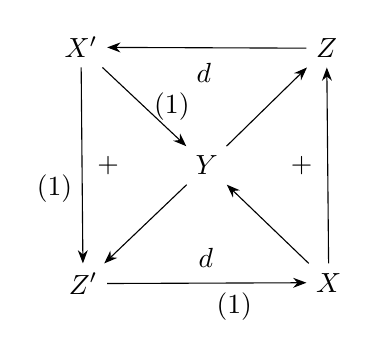
\begin{tikzpicture}[auto, >=Stealth, node distance=1cm and 1cm]

  % Define nodes
  \node (Y) {$Y$};
  \node (Xp) [above left=of Y] {$X'$};
  \node (X) [below right=of Y] {$X$};
  \node (Zp) [below left=of Y] {$Z'$};
  \node (Z) [above right=of Y] {$Z$};

  % Draw arrows
  \draw[->] (Z) to node [left] {} (Xp);
  \draw[->] (Y) to node [above right] {} (Z);
  \draw[->] (X) to node [below left] {} (Z);
  \draw[->] (X) to node [below left] {} (Y);
  \draw[->] (Zp) to node [below right] {\((1)\)} (X);
  \draw[->] (Xp) to node [ right] {\((1)\)} (Y);
  \draw[->] (Xp) to node [below left] {\((1)\)} (Zp);
  \draw[->] (Y) to node [below left] {} (Zp);

  % Add labels inside triangles
  \node at ($(Xp)!0.5!(Z)$) [below=2pt] {$d$};
  \node at ($(Zp)!0.5!(X)$) [above=2pt] {$d$};
  \node at ($(Xp)!0.5!(Zp)$) [right=2pt] {$+$};
  \node at ($(Z)!0.5!(X)$) [left=2pt] {$+$};
\end{tikzpicture}
\vspace{0.5em}{Upper Cap}
\end{minipage}
\begin{minipage}{0.45\textwidth}
\centering
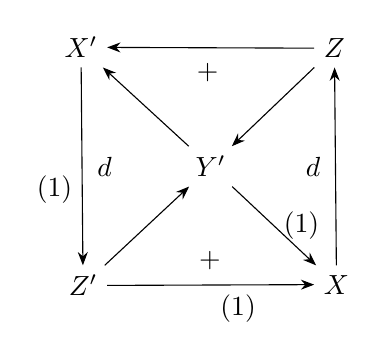
\begin{tikzpicture}[auto, >=Stealth, node distance=1cm and 1cm]
\usetikzlibrary{calc}
  % Define nodes
  \node (Y) {$Y'$};
  \node (Xp) [above left=of Y] {$X'$};
  \node (X) [below right=of Y] {$X$};
  \node (Zp) [below left=of Y] {$Z'$};
  \node (Z) [above right=of Y] {$Z$};

  % Draw arrows
  \draw[->] (Z) to node [left] {} (Xp);
  \draw[->] (Z) to node [above right] {} (Y);
  \draw[->] (X) to node [below left] {} (Z);
  \draw[->] (Y) to node [ right] {\((1)\)} (X);
  \draw[->] (Zp) to node [below right] {\((1)\)} (X);
  \draw[->] (Y) to node [below left] {} (Xp);
  \draw[->] (Xp) to node [below left] {\((1)\)} (Zp);
  \draw[->] (Zp) to node [below left] {} (Y);

  % Add labels inside triangles
  \node at ($(Xp)!0.5!(Z)$) [below=2pt] {$+$};
  \node at ($(Zp)!0.5!(X)$) [above=2pt] {$+$};
  \node at ($(Xp)!0.5!(Zp)$) [right=2pt] {$d$};
  \node at ($(Z)!0.5!(X)$) [left=2pt] {$d$};
\end{tikzpicture}
\vspace{0.5em}{Lower Cap}
\end{minipage}
\end{figure}
%% TRANSLATION-FIX: 1.1.6: neither a quarter turn nor the cap exchange alone is a symmetry; their composite is
The boundaries of these two squares coincide; the triangles marked \( + \) are commutative, and those marked \( d \) are distinguished. Furthermore, the composed arrows from \( Y \) to \( Y' \) via \( Z \) or \( Z' \), and those from \( Y' \) to \( Y \) via \( X \) or \( X' \), must also coincide. Ignoring arrow degrees, this diagram has a symmetry of order 4: it can be rotated a quarter turn while exchanging the upper and lower caps (cf. \rn{1.1.14}).

The TR 4 axiom for triangulated categories states that any diagram of the "upper cap" type can be completed into an octahedron diagram. The "upper cap" diagram represents the essence of distinguished triangles sharing a common vertex (completed by adding the composed arrows). The position of degree-$1$ arrows is imposed, but they can be changed by replacing vertices with their translates, using the TR 2 axiom to rotate distinguished triangles (careful with signs). For example, an axiom equivalent to TR 4 (modulo TR 1 to TR 3) is TR 4'. Any "lower cap" diagram can also be completed into a octahedron.

Up to isomorphism, providing an "upper cap" diagram amounts to providing \( X \to Y \to Z \) (constructing the distinguished triangles over \( u \) and \( v \); they are unique up to isomorphism). This also amounts to providing the upper cap, completed by the distinguished triangle \( (X, Z, Y') \). That the upper cap, completed by \( (X, Z, Y') \), can be extended into an octahedron is the formulation of TR 4 given in \cite{Verdier}.

\bbdhead{}{1.1.7} Illustration of Axiom TR 4.
In the case of the triangulated category \( K\mathcal{A} \) of Example \rn{1.1.2}, any filtered complex \( K \) with three levels
\[
0 = W_{-1} \subset W_0 \subset W_1 \subset W_2 = K,
\]
%% TRANSLATION-FIX: 1.1.7: Y' and Z' were interchanged (Z' = cone(X->Y) = W_1/W_0, Y' = cone(X->Z) = W_2/W_0)
where the filtration splits degree by degree, defines an octahedron, with vertices being the subquotients of \( K \) for the filtration \( W \): for \( X, Y, Z, X', Y', Z' \), take \( W_0, W_1, W_2, W_2/W_1, W_2/W_0, W_1/W_0 \) (where the boundary \( X, Z, X', Y, Z', Y' \) corresponds to \( \operatorname{Gr}_0K, \operatorname{Gr}_1K, \operatorname{Gr}_2K \)). The axiom results from the fact that any chain \( K \to L \to M \) of morphisms of complexes is isomorphic in \( K\mathcal{A} \) to a chain \( K' \to L' \to M' \) for which \( K'^i \to L'^i \) and \( L'^i \to M'^i \) are direct monomorphisms.

It is sometimes convenient to rewrite the octahedron diagram as follows:

{\begin{center}\begin{tikzpicture}[auto, >=Stealth]

  % Define coordinates for nodes
\node (Z) at (0, 0) {$Z$}; \node (Y) at (-1, 0.5) {$Y$}; \node (X) at (-2, -1) {$X$}; \node (Yp) at (1, 0.5) {$Y'$}; \node (Zp) at (0, 2) {$Z'$}; \node (Xp) at (2, -1) {$X'$}; \node (caption) at (-4, 0) {(1.1.7.1)}; \node (n1) at (0.83, 3.25) {$X[1]$}; \node (n2) at (2.34, 1.17) {$X[1]$}; \node (n3) at (3.61, -1.80) {$Y[1]$}; \node (n4) at (3.22, -2.83) {$Z'[1]$};

  % Draw arrows between nodes
\draw[->] (X) to node[midway, above left] {} (Z); \draw[->] (Y) to node[midway, above right] {} (Z); \draw[->] (X) to node[midway, below] {} (Y); \draw[->] (Z) to node[midway, below] {} (Yp); \draw[->] (Z) to node[midway, below] {} (Xp); \draw[->] (Y) to node[midway, below] {} (Zp); \draw[->] (Zp) to node[midway, below] {} (Yp); \draw[->] (Yp) to node[midway, below] {} (Xp); \draw[->] (Zp) to node[midway, below] {} (n1); \draw[->] (Yp) to node[midway, below] {} (n2); \draw[->] (Xp) to node[midway, below] {} (n3); \draw[->] (Xp) to node[midway, below] {} (n4);

\end{tikzpicture}
\end{center}}

This notation highlights the morphisms of distinguished triangles \( (X, Y, Z') \to (X, Z, Y') \to (Y, Z, X') \to (Z', Y', X') \)—except that for each of these morphisms, the corresponding commutative square is not explicit. A symmetry is, moreover, broken, so that the morphism of distinguished triangles \( (Z', Y', X') \to (Z', X[1], Y[1]) \), completing the preceding ones, is not explicit either.

\bbdhead{}{1.1.8}
We relate (1.1.7.1) to the fact that in an abelian category, two composable monomorphisms \( X \to Y \to Z \) give rise to a diagram of short exact sequences:

{\begin{center}\begin{tikzpicture}[auto, >=Stealth]

  % Define coordinates for nodes
\node (Z) at (0, 0) {$Z$}; \node (Y) at (-1, 0.5) {$Y$}; \node (X) at (-2, -1) {$X$}; \node (Yp) at (1, 0.5) {$Y'$}; \node (Zp) at (0, 2) {$Z'$}; \node (Xp) at (2, -1) {$X'$}; \node (caption) at (-4, 0) {(1.1.8.1)}; \node (n1) at (0.5, 2.75) {$0$}; \node (n2) at (2, 1) {$0$}; \node (n3) at (2.5, -1.75) {$0$}; \node (n4) at (3, -1.5) {$0$}; \node (n5) at (-0.5, 2.75) {$0$}; \node (n6) at (-2, 1) {$0$}; \node (n7) at (-2.5, -1.75) {$0$}; \node (n8) at (-3, -1.5) {$0$};

  % Draw arrows between nodes
\draw[->] (X) to node[midway, above left] {} (Z); \draw[->] (Y) to node[midway, above right] {} (Z); \draw[->] (X) to node[midway, below] {} (Y); \draw[->] (Z) to node[midway, below] {} (Yp); \draw[->] (Z) to node[midway, below] {} (Xp); \draw[->] (Y) to node[midway, below] {} (Zp); \draw[->] (Zp) to node[midway, below] {} (Yp); \draw[->] (Yp) to node[midway, below] {} (Xp); \draw[->] (Zp) to node[midway, below] {} (n1); \draw[->] (Yp) to node[midway, below] {} (n2); \draw[->] (Xp) to node[midway, below] {} (n3); \draw[->] (Xp) to node[midway, below] {} (n4); \draw[->] (n5) to node[midway, below] {} (Zp); \draw[->] (n6) to node[midway, below] {} (Y); \draw[->] (n7) to node[midway, below] {} (X); \draw[->] (n8) to node[midway, below] {} (X);

\end{tikzpicture}
\end{center}}

expressing that \( (Z/X)/(Y/X) = Z/Y \). The diagrams (1.1.7.1) and (1.1.8.1) are related as follows. Let a diagram (1.1.8.1) in the abelian category \( \mathcal{C}(\mathcal{A}) \) of complexes of objects in \( \mathcal{A} \). Each short exact sequence in \( \mathcal{C}(\mathcal{A}) \) defines a distinguished triangle in \( D(\mathcal{A}) \) (\cite[p.~31]{Verdier}), and the distinguished triangles derived from the short exact sequences in diagram (1.1.8.1) form an octahedron (1.1.7.1).

Here is a particular case. Identify the abelian category \( \mathcal{A} \) as a full subcategory of \( D\mathcal{A} \), via \( A \mapsto (A, 0) \) (the complex reduced to \( A \) in degree 0). For every short exact sequence \( 0 \to A \to B \to C \to 0 \) in \( \mathcal{A} \), there exists one and only one degree 1 arrow \( C \to A[1] \) such that the triangle \( A \to B \to C \to A[1] \) is distinguished: the existence of this triangle is a particular case of the fact that every short exact sequence of complexes determines a distinguished triangle (\cite[p.~31]{Verdier}), and its uniqueness results from \rn{1.1.10} below, and from the fact that for \( A \) and \( B \) in \( \mathcal{A} \), \( \operatorname{Hom}^n(A, B) = 0 \) for \( n < 0 \) (for \( n \ge 0 \), this is the $n$-th \( \operatorname{Ext} \) group of Yoneda from \( A \) to \( B \)). If we take a diagram (1.1.8.1) in \( \mathcal{A} \), and complete each of its short exact sequences into a distinguished triangle in \( D\mathcal{A} \), we obtain a diagram (1.1.7.1). This is a consequence of TR 4.

\bbdhead{Proposition}{1.1.9} \emph{Let} \( (X, Y, Z) \) \emph{and} \( (X', Y', Z') \) \emph{be two distinguished triangles, and let} \( g: Y \to Y' \):

\[
\begin{array}{cccccc}
X & \xrightarrow{u} & Y & \xrightarrow{v} & Z & \xrightarrow{d} \\
f \dashdownarrow & (1) & g \downarrow & (2) & h \dashdownarrow & \\
X' & \xrightarrow{u'} & Y' & \xrightarrow{v'} & Z' & \xrightarrow{d'} \\
\end{array}
\]

\emph{The following conditions are equivalent:}

%% TRANSLATION-FIX: 1.1.9(a): v'g and u' are not composable; the condition is v'gu = 0
\emph{(a)} \( v'gu = 0 \),

\emph{(b) there exists} \( f \) \emph{making square (1) commute,}

\emph{(b')} \emph{there exists} \( h \) \emph{making square (2) commute,}

\emph{(c) there exists a morphism of triangles} \( (f, g, h) \).

\emph{If these conditions are satisfied, and} \( \operatorname{Hom}^{-1}(X, Z') = 0 \), \emph{the morphism} \( f \) \emph{(resp.} \( h \)\emph{) in (b) (resp. b') is unique.}

The exactness of the sequence
\[
\operatorname{Hom}^{-1}(X, Z') \to \operatorname{Hom}(X, X') \to \operatorname{Hom}(X, Y') \to \operatorname{Hom}(X, Z'),
\]
%% TRANSLATION-FIX: 1.1.9: TR 2 is rotation; producing h from a commutative square is TR 3
applied to \( g \circ u\) in \( \operatorname{Hom}(X, Y') \), shows that (a) \( \Leftrightarrow \) (b), with uniqueness of \( f \) if \( \operatorname{Hom}^{-1}(X, Z') = 0 \). That (b) \( \Rightarrow \) (c) results from TR 3: if \( f \) satisfies (b), there exists \( h \) such that \((f, g, h)\) is a morphism of triangles. The reciprocal is trivial. Finally, a dual argument gives \( (a) \Leftrightarrow (b') \), and the uniqueness of \( h \) if \( \operatorname{Hom}^{-1}(X, Z') = 0 \).

\bbdhead{Corollary}{1.1.10}
\emph{Let \( X \overset{u}\to Y \overset{v}\to Z \overset{d}\to \) be a distinguished triangle. If \( \operatorname{Hom}^{-1}(X, Z) = 0 \), then:
\begin{itemize}
\item[(i)] the cone of \( u \) is unique up to unique isomorphism;
\item[(ii)] \( d \) is the unique morphism \( x: Z \to X[1] \) such that the triangle \( X \overset{u}\to Y \overset{v}\to Z \overset{x}\to X[1] \) is distinguished.
\end{itemize}}

If in \rn{1.1.9}, \( X = X' \), \( Y = Y' \), and \( f, g \) are identical, \( Z \) is isomorphic to \( Z' \), from which \( \operatorname{Hom}^{-1}(X, Z') = 0 \). Then (i) follows from the uniqueness of \( h \). For (ii), we apply \rn{1.1.9} to:

\[
\begin{array}{cccccc}
X & \xrightarrow{u} & Y & \xrightarrow{v} & Z & \xrightarrow{d} \\
\| &  & \| &  & & \\
X & \xrightarrow{u} & Y & \xrightarrow{v} & Z & \xrightarrow{x} \\
\end{array}
\]

We necessarily have \( h = \operatorname{id}_Z \), hence \( d = x \).

Dually, in \rn{1.1.10}, the cone of \( v \) is unique up to isomorphism.

This proposition was pointed out to us by J.L. Verdier.
\bbdhead{Proposition}{1.1.11}
\emph{ Any commutative square \( (X' \to Y') \to (X \to Y) \) can be completed into a diagram of 9:}

\[\begin{array}{ccccccccc}
X'[1] & \dashrightarrow & Y'[1] & \dashrightarrow & Z'[1] & \dashrightarrow & X'[2] \\
\uparrow & & \uparrow & & \uparrow & & \uparrow \\
X'' & \to & Y'' & \to & Z'' & \to & X''[1] \\
\uparrow & & \uparrow & & \uparrow & & \uparrow \\
X & \to & Y & \to & Z & \to & X[1] \\
\uparrow & & \uparrow & & \uparrow & & \uparrow \\
X' & \to & Y' & \to & Z' & \to & X'[1] \\
\end{array}\]

\emph{In this diagram, the dotted arrows are deduced from the solid arrows by applying the translation functor. The squares are commutative except for the one marked \( - \), which is anticommutative, and the rows and columns of solid lines are distinguished triangles.}

%% TRANSLATION-FIX: 1.1.11: the columns of the nine-diagram are (X',X,X'') and (Y',Y,Y''); X' -> Y is the diagonal
We choose distinguished triangles \( (X', Y', Z') \), \( (X, Y, Z) \), \( (X', X, X'') \), \( (Y', Y, Y'') \) on the sides of the commutative square, and \( (X', Y, A) \) on its diagonal \( X' \to Y \). The TR 4 axiom allows completing the following octahedra:
\begin{figure}[h!]
\centering
\begin{minipage}{0.45\textwidth}
\centering
\begin{tikzpicture}[auto, >=Stealth, scale=0.8, transform shape]

  % Define coordinates for nodes
  \node (Z) at (0, 0) {$Y$};
  \node (Y) at (-1, 0.5) {$Y'$};
  \node (X) at (-2, -1) {$X'$};
  \node (Yp) at (1, 0.5) {$A$};
  \node (Zp) at (0, 2) {$Z'$};
  \node (Xp) at (2, -1) {$Y''$};
  \node (caption) at (-3, 0) {(1)};
  \node (n1) at (0.83, 3.25) {$X'[1]$};
  \node (n2) at (2.34, 1.17) {$X'[1]$};
  \node (n3) at (3.61, -1.80) {$Y'[1]$};
  \node (n4) at (3.22, -2.83) {$Z'[1]$};

  % Draw arrows between nodes
  \draw[->] (X) to node[midway, above left] {} (Z);
  \draw[->] (Y) to node[midway, above right] {} (Z);
  \draw[->] (X) to node[midway, below] {} (Y);
  \draw[->] (Z) to node[midway, below] {} (Yp);
  \draw[->] (Z) to node[midway, below] {} (Xp);
  \draw[->] (Y) to node[midway, below] {} (Zp);
  \draw[->] (Zp) to node[midway, below] {} (Yp);
  \draw[->] (Yp) to node[midway, below] {} (Xp);
  \draw[->] (Zp) to node[midway, below] {} (n1);
  \draw[->] (Yp) to node[midway, below] {} (n2);
  \draw[->] (Xp) to node[midway, below] {} (n3);
  \draw[->] (Xp) to node[midway, below] {} (n4);
\end{tikzpicture}
\(\text{Based on } X' \to Y' \to Y\)
\end{minipage}
\begin{minipage}{0.45\textwidth}
\centering
\begin{tikzpicture}[auto, >=Stealth, scale=0.8, transform shape]

  % Define coordinates for nodes
  \node (Z) at (0, 0) {$Y$};
  \node (Y) at (-1, 0.5) {$X$};
  \node (X) at (-2, -1) {$X'$};
  \node (Yp) at (1, 0.5) {$A$};
  \node (Zp) at (0, 2) {$X''$};
  \node (Xp) at (2, -1) {$Z$};
  \node (caption) at (-3, 0) {(2)};
  \node (n1) at (0.83, 3.25) {$X'[1]$};
  \node (n2) at (2.34, 1.17) {$X'[1]$};
  \node (n3) at (3.61, -1.80) {$X[1]$};
  \node (n4) at (3.22, -2.83) {$X''[1]$};

  % Draw arrows between nodes
  \draw[->] (X) to node[midway, above left] {} (Z);
  \draw[->] (Y) to node[midway, above right] {} (Z);
  \draw[->] (X) to node[midway, below] {} (Y);
  \draw[->] (Z) to node[midway, below] {} (Yp);
  \draw[->] (Z) to node[midway, below] {} (Xp);
  \draw[->] (Y) to node[midway, below] {} (Zp);
  \draw[->] (Zp) to node[midway, below] {} (Yp);
  \draw[->] (Yp) to node[midway, below] {} (Xp);
  \draw[->] (Zp) to node[midway, below] {} (n1);
  \draw[->] (Yp) to node[midway, below] {} (n2);
  \draw[->] (Xp) to node[midway, below] {} (n3);
  \draw[->] (Xp) to node[midway, below] {} (n4);

\end{tikzpicture}
\(\text{Based on } X' \to X \to Y\)
\end{minipage}
\end{figure}

\newpage then the octahedron
\begin{center}\begin{minipage}{0.45\textwidth}
\centering
\begin{tikzpicture}[auto, >=Stealth, scale=0.8, transform shape]

  % Define coordinates for nodes
  \node (Z) at (0, 0) {$Y''$};
  \node (Y) at (-1, 0.5) {$A$};
  \node (X) at (-2, -1) {$X''$};
  \node (Yp) at (1, 0.5) {$Z''$};
  \node (Zp) at (0, 2) {$Z$};
  \node (Xp) at (2, -1) {$Z'[1]$};
  \node (caption) at (-3, 0) {(3)};
  \node (n1) at (0.83, 3.25) {$X''[1]$};
  \node (n2) at (2.34, 1.17) {$X''[1]$};
  \node (n3) at (3.61, -1.80) {$A[1]$};
  \node (n4) at (3.22, -2.83) {$Z[1]$};

  % Draw arrows between nodes
  \draw[->] (X) to node[midway, above left] {} (Z);
  \draw[->] (Y) to node[midway, above right] {} (Z);
  \draw[->] (X) to node[midway, below] {} (Y);
  \draw[->] (Z) to node[midway, below] {} (Yp);
  \draw[->] (Z) to node[midway, below] {} (Xp);
  \draw[->] (Y) to node[midway, below] {} (Zp);
  \draw[->] (Zp) to node[midway, below] {} (Yp);
  \draw[->] (Yp) to node[midway, below] {} (Xp);
  \draw[->] (Zp) to node[midway, below] {} (n1);
  \draw[->] (Yp) to node[midway, below] {} (n2);
  \draw[->] (Xp) to node[midway, below] {} (n3);
  \draw[->] (Xp) to node[midway, below] {} (n4);
\end{tikzpicture}
\(\text{Based on } X'' \to A \to Y''\)
\end{minipage}
\end{center}

where the distinguished triangle \( (A, Y", Z'[1]) \) is deduced by rotation from \( (Z', A, Y") \) in diagram (1): the sign of the arrow \( Z' \to A \) is changed.

The required distinguished triangles appear in these octahedra (except that \( (Z', Z, Z'') \) appears as \( (Z, Z'', Z'[1]) \); one deduces \( (Z', Z, Z'') \) from \( (Z, Z'', Z'[1]) \) by changing the sign of the arrow \( Z' \to Z \)).

%% TRANSLATION-FIX: 1.1.11: the column triangles send X'',Y'',Z'' to X'[1],Y'[1],Z'[1]
%% TRANSLATION-FIX: 1.1.11: the target triangle mixed unprimed X[1],Y[1] with primed Z'[1]
%% TRANSLATION-FIX: 1.1.11: octahedron (1) is based on X' -> Y' -> Y, so its fourth morphism targets (Z',X'[1],Y'[1])
To prove the required (anti-)commutativity, we observe that the arrows \( X', Y', Z' \) in \( X, Y, Z \) constitute the composition of the morphisms of triangles \( (X', Y', Z') \to (X', Y, A) \to (X, Y, Z) \) appearing in (1) and (2); the arrows \( X, Y, Z \) in \( X", Y", Z" \) constitute the composition of the morphisms of triangles \( (X, Y, Z) \to (X", A, Z) \to (X", Y", Z") \), and the arrows \( X", Y", Z" \) in \( X'[1], Y'[1], Z'[1] \) constitute the composition of the morphisms of triangles \( (X", Y", Z") \to (A, Y", Z'[1]) \to (X'[1], Y'[1], Z'[1]) \), where the last arrow is deduced by rotation of the morphism of triangles from (1): \( (Z', A, Y") \to (Z', X'[1], Y'[1]) \). In the distinguished triangle \( (X'[1], Y'[1], Z'[1]) \), the degree 1 arrow differs in sign from the translation of the degree 1 arrow of the triangle \( (X', Y', Z') \), which explains the anticommutativity of the 9th square.

\bbdhead{Remark}{1.1.12}
A square of short exact sequences of complexes defines a 9-diagram in the derived category. The anticommutativity of the 9th square specifies the anticommutativity of the corresponding coboundaries.

\bbdhead{Remark}{1.1.13}
In usual triangulated categories (e.g., \( K\mathcal{A} \) for \( \mathcal{A} \) additive, \( D\mathcal{A} \) for \( \mathcal{A} \) exact, the stable homotopy category, etc.), any diagram of the "upper cap" type of an octahedron can be completed into an octahedron where the following triangles are distinguished:

\[
Y \to Y' \to X' \oplus X[1] \overset{(1)}{\to} Y, \text{and}
\]
\[
Y \to Z \oplus Z' \to Y' \overset{(1)}\to Y.
\]

(The arrows are those of the octahedron, except for \( Y' \to X[1] \) and \( Z' \to Y' \), which are opposite to those of the octahedron). We do not know if this is generally the case. If these triangles become useful, it may be appropriate to strengthen axiom TR 4 of triangulated categories by redefining "octahedron" so that these triangles are distinguished by definition of the octahedra.

\bbdhead{Remark}{1.1.14}
The diagrams of the triangle and the octahedron allow the following generalization, of which the particular cases are obtained for \( N = 3 \) and \( N = 4 \). For \( N \geq 2 \), the diagram consists of:
\begin{itemize}
\item[(a)] For each interval \( I \) of \( \mathbb{Z} \), with \( 0 \leq \# I < N \), the data of \( K(I) \).
%% TRANSLATION-FIX: 1.1.14(b): transitivity is phi_KJ phi_JI = phi_KI; as printed the composite is not defined
\item[(b)] For \( I = [a, b[ \) and \( J = [c, d[ \), define \( I \leq J \) such that \( a \leq c \) and \( b \leq d \). We give arrows \( \varphi_{JI} : K(I) \to K(J) \), for \( I \leq J \), such that \( \varphi_{KJ} \varphi_{JI} = \varphi_{KI} \) and \( \varphi_{II} = \text{id} \). For \( I = [a, b[ \), \( J = [c, d[ \) and \( b \leq c \), \( \varphi_{JI} = 0 \).
\item[(c)] For \( I = [a, b[ \), define \( I^* = [b, a+N[ \). We give isomorphisms \( K(I^*) = K(I)[1] \) that, for \( I \leq J \), make the diagram commute:
    \[
    \begin{array}{ccc}
    K(I)[1] & \rightarrow & K(J)[1] \\
%% TRANSLATION-FIX: 1.1.14(c): phi_{JI^*} is not a defined arrow; the verticals are the isomorphisms of (c)
    \quad\downarrow {\scriptstyle \wr}  & & \downarrow{\scriptstyle \wr} \\
    K(I^*) & \rightarrow & K(J^*).
    \end{array}
    \]
\item[(d)] For \( a < b < c < a+N \), the triangle of arrows \( \varphi : K([a, b[) \to K([a, c[) \to K([b, c[) \to K([a, b[)[1] \) is distinguished.
\end{itemize}

A filtered complex with \( (N-1) \) levels, with degree-by-degree splittable filtration, defines such a diagram in \( K\mathcal{A} \). If the filtration \( W \) of \( K \) is taken as increasing, with \( W_0K = 0 \) and \( W_{N-1}K = K \) (i.e., \( \operatorname{Gr}^W_i K = 0 \) for \( i \notin [1, N-1] \)), then one sets \( K([a, b[) = W_{b-1}K/W_{a-1}K \) for \( 1 \leq a < b \leq N \) and \( K(\{ 0 \}) = K[-1] \).

\section{Abelian Subcategories}

\bbdhead{}{1.2.0}
Let \( \mathcal{D} \) be a triangulated category and \( \mathcal{C} \) a full subcategory of \( \mathcal{D} \). We assume that \( \operatorname{Hom}^i(X, Y) := \operatorname{Hom}(X, Y[i]) \) is zero for \( i < 0 \) and \( X, Y \in \mathcal{C} \).

\bbdhead{Example}{1.2.1}
\( \mathcal{D} \) is the derived category of an abelian category \( \mathcal{A} \), and \( \mathcal{C} = \mathcal{A} \), identified with a full subcategory of \( \mathcal{D} \) via the functor \( A \mapsto A \) (the complex reduced to \( A \) in degree 0).

\bbdhead{Proposition}{1.2.2}
\emph{Let \( f: X \to Y \) be in \( \mathcal{C} \). Complete \( f \) into a distinguished triangle \( X \xrightarrow{f} Y \to S \to X[1] \), and suppose \( S \) appears in a distinguished triangle \( N[1] \to S \to C \to N[2] \), with \( N, C \in \mathcal{C} \):}

\begin{minipage}{0.45\textwidth}
\centering
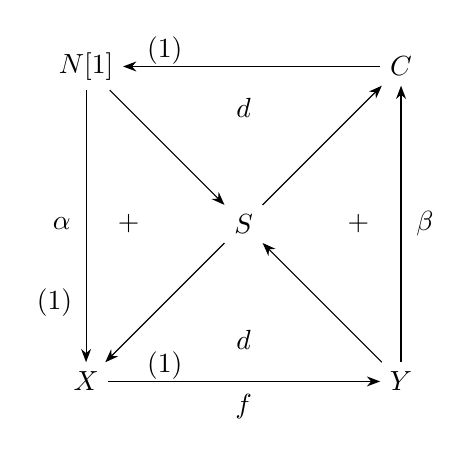
\begin{tikzpicture}[auto, >=Stealth, node distance=1cm and 1cm]

  % Define nodes

  \node (Y) at (0, 0) {$S$};
  \node (Xp) at (-2, 2) {$N[1]$};
  \node (X) at (2, -2) {$Y$};
  \node (Zp) at (-2, -2) {$X$};
  \node (Z) at (2, 2) {$C$};
  \node (n1) at (-1, 2.2) {$(1)$};
  \node (n2) at (-2.4, -1) {$(1)$};
  \node (n3) at (-1, -1.8) {$(1)$};
  % Draw arrows
  \draw[->] (Z) to node [above left] {} (Xp);
  \draw[->] (Y) to node [above right] {} (Z);
  \draw[->] (X) to node [below left] {} (Z);
  \draw[->] (X) to node [below left] {} (Y);
  \draw[->] (Zp) to node [above left] {} (X);
  \draw[->] (Xp) to node [ right] {} (Y);
  \draw[->] (Xp) to node [below left] {} (Zp);
  \draw[->] (Y) to node [below left] {} (Zp);

  % Add labels inside triangles
  \node at ($(Xp)!0.5!(Z)$) [below=8pt] {$d$};
  \node at ($(Zp)!0.5!(X)$) [above=8pt] {$d$};
  \node at ($(Zp)!0.5!(X)$) [below=1pt] {$f$};
  \node at ($(Xp)!0.5!(Zp)$) [right=8pt] {$+$};
  \node at ($(Z)!0.5!(X)$) [left=8pt] {$+$};
  \node at ($(Xp)!0.5!(Zp)$) [left=2pt] {$\alpha$};
  \node at ($(Z)!0.5!(X)$) [right=2pt] {$\beta$};
\end{tikzpicture}
\end{minipage}
\begin{minipage}{0.45\textwidth}

\emph{(where the triangles marked \( + \) are commutative and those marked \( d \) are distinguished).}
\end{minipage}
\emph{Then \( \alpha[-1]: N \to X \) is a kernel of \( f \) in \( \mathcal{C} \), and \( \beta: Y \to C \) is a cokernel of \( f \).}

For \( Z \in \mathcal{C} \), the long exact sequence of \( \operatorname{Hom} \) provides, thanks to \rn{1.2.0}, the exact sequences:
\[
0 \to \operatorname{Hom}^{-1}(Z, S) \to \operatorname{Hom}(Z, X) \to \operatorname{Hom}(Z, Y),
\text{ and}\]
\[
0 \to \operatorname{Hom}(Z, N) \to \operatorname{Hom}^{-1}(Z, S) \to 0.
\]
These show that \( (N, \alpha[-1]) \) is a kernel of \( f \). A dual argument shows that \( (C, \beta) \) is a cokernel.

\paragraph{Example.}
For \( \mathcal{A} = D(\mathcal{A}) \) (Example \rn{1.2.1}), the cone \( S \) of \( f: X \to Y \) is the complex \( X \xrightarrow{f} Y \) (in degree -1 and 0). It admits as subcomplex \( \operatorname{Ker}(f)[1] = H^{-1}(S)[1] \), and the quotient \( X/\operatorname{Ker}(f) \to Y \) maps quasi-isomorphically onto \( \operatorname{Coker}(f) = H^0(S) \) placed in degree 0. One has the diagram (1.2.2.1).

\bbdhead{}{1.2.3}
%% TRANSLATION-FIX: 1.2.3: f mono means N = 0 and gives the triangle (X,Y,C); f epi means C = 0
A morphism \( f: X \to Y \) in \( \mathcal{C} \) is called \( \mathcal{C} \)-\emph{admissible}, or simply \emph{admissible}, if there is no ambiguity on \( \mathcal{C} \), if it is the base of a diagram (1.2.2.1). If \( f \) is a monomorphism, \( N = 0 \), so \( S \cong C \), and (1.2.2.1) reduces to a distinguished triangle \( (X, Y, C) \). If \( f \) is an epimorphism, \( C = 0 \), so \( N[1] \cong S \), and (1.2.2.1) reduces to a distinguished triangle \( (N, X, Y) \). Reciprocally, for every distinguished triangle \( X \overset{f}\to Y \overset{g}\to Z \overset{d}\to X[1] \), with \( X, Y, Z \in \mathcal{C} \), \( f \) and \( g \) are admissible, \( f \) is a kernel of \( g \), and \( g \) is a cokernel of \( f \). By \rn{1.2.0} and \rn{1.1.10}, \( d \) is determined by \( f \) and \( g \).

A sequence \( X \to Y \to Z \) in \( \mathcal{C} \) is a \emph{short exact admissible sequence} if it is deduced from a distinguished triangle by removing the degree 1 arrow.

\bbdhead{Proposition}{1.2.4}\footnote{\emph{Errata and Addenda} (2018), item~6: For the assertion \emph{Conversely\dots} one needs that $0\in\mathcal{C}$ (more precisely, that some zero object is in $\mathcal{C}$). Counterexample: $\mathcal{D}=D^{b}(k)$ for $k$ a field, $\mathcal{C}$ the category of non-zero vector spaces.}
\emph{Assume \( \mathcal{C} \) is stable under finite direct sums. The following conditions are equivalent:\emph}
\begin{itemize}
\item[(i)] \emph{\( \mathcal{C} \) is abelian, and its short exact sequences are admissible.}
\item[(ii)] \emph{Every morphism in \( \mathcal{C} \) is \( \mathcal{C} \)-admissible.}
\end{itemize}

\paragraph{Proof.}
Let us show \( (ii) \implies (i) \). By \rn{1.2.2}, every morphism in \( \mathcal{C} \) has a kernel and cokernel. To prove \( \mathcal{C} \) is abelian, it remains to verify that \( \operatorname{Coim}(f) \cong \operatorname{Im}(f) \). Consider diagram (1.2.2.1) as the lower cap of an octahedron and apply TR 4' (cf. \rn{1.1.7}) to complete it into an octahedron:

\begin{minipage}{0.45\textwidth}
\centering
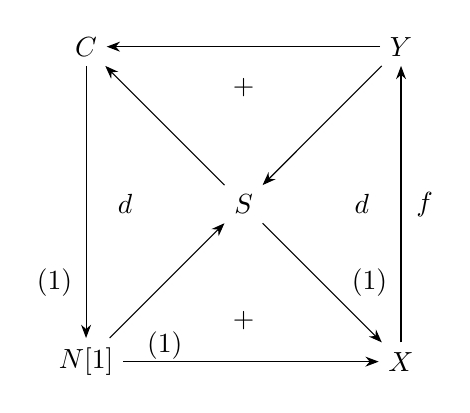
\begin{tikzpicture}[auto, >=Stealth, node distance=1cm and 1cm]

  % Define nodes

  \node (Y) at (0, 0) {$S$};
  \node (Xp) at (-2, 2) {$C$};
  \node (X) at (2, -2) {$X$};
  \node (Zp) at (-2, -2) {$N[1]$};
  \node (Z) at (2, 2) {$Y$};
  \node (n1) at (-2.4, -1) {$(1)$};
  \node (n2) at (1.6, -1) {$(1)$};
  \node (n3) at (-1, -1.8) {$(1)$};
  % Draw arrows
  \draw[->] (Z) to node [above left] {} (Xp);
  \draw[->] (Z) to node [above right] {} (Y);
  \draw[->] (X) to node [below left] {} (Z);
  \draw[->] (Y) to node [below left] {} (X);
  \draw[->] (Zp) to node [above left] {} (X);
  \draw[->] (Y) to node [ right] {} (Xp);
  \draw[->] (Xp) to node [below left] {} (Zp);
  \draw[->] (Zp) to node [below left] {} (Y);

  % Add labels inside triangles
  \node at ($(Xp)!0.5!(Z)$) [below=8pt] {$+$};
  \node at ($(Zp)!0.5!(X)$) [above=8pt] {$+$};
  \node at ($(Xp)!0.5!(Zp)$) [right=8pt] {$d$};
  \node at ($(Z)!0.5!(X)$) [left=8pt] {$d$};
  \node at ($(Z)!0.5!(X)$) [right=2pt] {$f$};
\end{tikzpicture}
\end{minipage}
\begin{minipage}{0.45\textwidth}
\centering
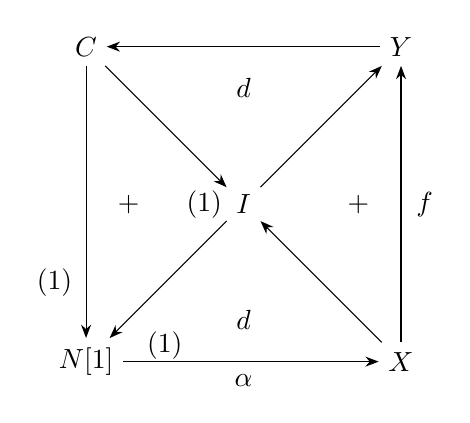
\begin{tikzpicture}[auto, >=Stealth, node distance=1cm and 1cm]

  % Define nodes

  \node (Y) at (0, 0) {$I$};
  \node (Xp) at (-2, 2) {$C$};
  \node (X) at (2, -2) {$X$};
  \node (Zp) at (-2, -2) {$N[1]$};
  \node (Z) at (2, 2) {$Y$};
  \node (n1) at (-0.5, 0) {$(1)$};
  \node (n2) at (-2.4, -1) {$(1)$};
  \node (n3) at (-1, -1.8) {$(1)$};
  % Draw arrows
  \draw[->] (Z) to node [above left] {} (Xp);
  \draw[->] (Y) to node [above right] {} (Z);
  \draw[->] (X) to node [below left] {} (Z);
  \draw[->] (X) to node [below left] {} (Y);
  \draw[->] (Zp) to node [above left] {} (X);
  \draw[->] (Xp) to node [ right] {} (Y);
  \draw[->] (Xp) to node [below left] {} (Zp);
  \draw[->] (Y) to node [below left] {} (Zp);

  % Add labels inside triangles
  \node at ($(Xp)!0.5!(Z)$) [below=8pt] {$d$};
  \node at ($(Zp)!0.5!(X)$) [above=8pt] {$d$};
  \node at ($(Zp)!0.5!(X)$) [below=1pt] {$\alpha$};
  \node at ($(Xp)!0.5!(Zp)$) [right=8pt] {$+$};
  \node at ($(Z)!0.5!(X)$) [left=8pt] {$+$};
  \node at ($(Xp)!0.5!(Zp)$) [left=2pt] {};
  \node at ($(Z)!0.5!(X)$) [right=2pt] {$f$};
\end{tikzpicture}
\end{minipage}

By \rn{1.2.2}, \( \beta \) is an epimorphism, as a cokernel of \( f \). By \rn{1.2.3}, the triangle \( (I, Y, C) \) is distinguished, \( I \in \mathcal{C} \), and \( I \) is the image of \( f \). Dually, the distinguished triangle \( (N, X, I) \), deduced by rotation of the other distinguished triangle of the upper cap, shows that \( I \) is the coimage of \( f \). Finally, by \rn{1.2.3}, the short exact sequences in \( \mathcal{C} \) are admissible.

Let us show \( (i) \implies (ii) \). The kernel \( N \), cokernel \( C \), and image \( I \) of \( f: X \to Y \) yield two short exact sequences \( 0 \to N \to X \to I \to 0 \) and \( 0 \to I \to Y \to C \to 0 \), that is, two triangles forming the upper cap diagram above. Applying TR 4, we deduce the lower cap: \( f \) is admissible.

\bbdhead{Definition}{1.2.5}
A full subcategory \( \mathcal{C} \) of \( \mathcal{D} \) is \emph{abelian-admissible} if it satisfies \rn{1.2.0} and the equivalent conditions of \rn{1.2.4}.

\bbdhead{}{1.2.6}
In a triangulated category \( \mathcal{D} \), we will sometimes say that an object \( Y \) is an extension of \( Z \) by \( X \) if there exists a distinguished triangle \( (X, Y, Z) \). A full subcategory \( \mathcal{D}' \) of \( \mathcal{D} \) is stable under extensions if for any distinguished triangle \( (X, Y, Z) \) with \( X \) and \( Z \) in \( \mathcal{D}' \), \( Y \) is also in \( \mathcal{D}' \).

\section{t-Categories}

\bbdhead{Definition}{1.3.1}
%% TRANSLATION-FIX: 1.3.1: a t-structure is a pair (D^{<=0}, D^{>=0}); D^{<0} is never a datum
A t-category is a triangulated category \( \mathcal{D} \), equipped with two strictly full subcategories \( \mathcal{D}^{\leq 0} \) and \( \mathcal{D}^{\geq 0} \), such that, setting \( \mathcal{D}^{\leq n} := \mathcal{D}^{\leq 0}[-n] \) and \( \mathcal{D}^{\geq n} := \mathcal{D}^{\geq 0}[-n] \), we have:
\begin{itemize}
%% TRANSLATION-FIX: 1.3.1(i): the orthogonality axiom is for X in D^{<=0}
\item[(i)] For \( X \in \mathcal{D}^{\leq 0} \) and \( Y \in \mathcal{D}^{\geq 1} \), \( \operatorname{Hom}(X, Y) = 0 \).
%% TRANSLATION-FIX: 1.3.1(ii): as printed the axiom is vacuous; it is the nesting condition
\item[(ii)] \( \mathcal{D}^{\leq 0} \subseteq \mathcal{D}^{\leq 1} \) and \( \mathcal{D}^{\geq 1} \subseteq \mathcal{D}^{\geq 0} \).
%% TRANSLATION-FIX: 1.3.1(iii): the third vertex must lie in D^{>=1}, else A=0, B=X satisfies the axiom always
\item[(iii)] For any \( X \in \mathcal{D} \), there exists a distinguished triangle \( A \to X \to B \to A[1] \), with \( A \in \mathcal{D}^{\leq 0} \) and \( B \in \mathcal{D}^{\geq 1} \).
\end{itemize}

%% TRANSLATION-FIX: 1.3.1: the heart is D^{<=0} cap D^{>=0}, as written at 1.3.6
We also say that \( (\mathcal{D}^{\leq 0}, \mathcal{D}^{\geq 0}) \) is a t-structure on \( \mathcal{D} \). Its heart is the full subcategory \( \mathcal{C} := \mathcal{D}^{\leq 0} \cap \mathcal{D}^{\geq 0} \).

\bbdhead{Examples}{1.3.2}
\begin{itemize}
\item[(i)] Let \(A\) be an abelian category. The natural t-structure on \(D(A)\) is the one where \((D(A))^{\le n}\) (resp. \((D(A))^{\geq n}\)) is the subcategory of complexes \(K\) such that \(H^i(K) = 0\) for \(i > n\) (resp. \(i < n\)), i.e., quasi-isomorphic to a complex \(K'\) null in degrees \(> n\) (resp. \(< n\)).

Let us verify \(1.3.1.(iii)\). For any complex \(K\), the truncation \(\tau_{\le 0}K\) is the subcomplex:
   \[
   \cdots \to K^{-1} \to \ker(d^0) \to 0 \to \cdots
   \]
of \(K\). Note that, in \cite{Hartshorne}, this truncation is denoted \(\sigma_{\le 0}K\). In \cite{Illusie}, it is denoted \(t_{0]}K\).

Define \(\tau_{\ge1}K := K/\tau_{\le0}K\). We have \(\tau_{\le0}K \in (D(A))^{\le 0}\), \(\tau_{\ge1}K \in (D(A))^{\geq 1}\), and the short exact sequence:
   \[
   0 \to \tau_{\le0}K \to K \to \tau_{\ge1}K \to 0
   \]
provides the required triangle. The verification of conditions \(1.3.1.(i)\) and \(1.3.1.(ii)\) is left to the reader.

\item[(ii)] If \( (\mathcal{D}^{\le 0}, \mathcal{D}^{\geq 0}) \) is a t-structure on \( \mathcal{D} \), then for every integer \( n \), \( (\mathcal{D}^{\le n}, \mathcal{D}^{\geq n}) \) is another t-structure, derived from the first by translation.
%% TRANSLATION-FIX: 1.3.2(iii): D^{<0} for D^{<=0} in the dual t-structure
\item[(iii)] If \( (\mathcal{D}^{\leq 0}, \mathcal{D}^{\geq 0}) \) is a t-structure on \( \mathcal{D} \), then \( (\mathcal{D}^{\geq 0}_{\text{opp}}, \mathcal{D}^{\leq 0}_{\text{opp}}) \) is a t-structure, called the dual t-structure, on the opposite triangulated category \( \mathcal{D}_{\text{opp}} \). This will allow reasoning by duality (a statement is dual to another if it is obtained by applying the latter to the opposite category).
\end{itemize}

Let \( \mathcal{D} \) be a t-category.

\bbdhead{Proposition}{1.3.3}
\begin{itemize}
%% TRANSLATION-FIX: 1.3.3(i): D^{<n} for D^{<=n}
\item[(i)] The inclusion \( \mathcal{D}^{\leq n} \to \mathcal{D} \) admits a right adjoint \( \tau_{\le n} \), and \( \mathcal{D}^{\geq n} \to \mathcal{D} \) admits a left adjoint \( \tau_{\geq n} \).
\item[(ii)] For any \( X \in \mathcal{D} \), there exists a unique morphism \( d \in \operatorname{Hom}^1(\tau_{\geq 1}X, \tau_{\le 0}X) \) such that the triangle:
    \[
    \tau_{\le 0}X \to X \to \tau_{\geq 1}X \xrightarrow{d}
    \]
is distinguished. Up to a unique isomorphism, this triangle is the only distinguished triangle \((A, X, B)\) with \(A\) in \(D^{\le 0}\) and \(B\) in \(D^{\ge 1}\).
\end{itemize}

By duality and translation, it suffices to verify (i) for \(D_{\leq 0}\). For every \(X\) in \(D\), we need to find \(A\) in \(D_{\leq 0}\), equipped with \(A \to X\) (the value of \(\tau_{\leq 0}\) on \(X\)), such that for all \(T\) in \(D_{\leq 0}\), we have
\[
\mathrm{Hom}(T, A) \to \mathrm{Hom}(T, X).
\]
%% TRANSLATION-FIX: 1.3.3: a map cannot 'imply'; what the exact sequence gives is that it is bijective
Let \((A, X, B)\) be a triangle as in \rn{1.3.1} (iii). The long exact sequence of \(\mathrm{Hom}\)'s and the conditions in \rn{1.3.1} (i)(ii) show that \(\mathrm{Hom}(T, A) \to \mathrm{Hom}(T, X)\) is bijective. This proves (i), the existence of a distinguished triangle \((\tau_{\leq 0} X, X, \tau_{\geq 1} X)\), and the fact that every distinguished triangle as in \rn{1.3.1} (iii) \((A, X, B)\) is uniquely isomorphic to this triangle, after forgetting the degree 1 arrow. The uniqueness of this latter follows from \rn{1.3.1} (i)(ii) and \rn{1.1.10} (ii).
\bbdhead{}{1.3.4}
The distinguished triangle \((\tau_{\leq 0} X, X, \tau_{\geq 1} X)\) shows that the following conditions are equivalent: (a) \(\tau_{\leq 0} X = 0\), i.e., (a') \(\mathrm{Hom}(T, X) = 0\) for all \(T\) in \(D^{\leq 0}\); (b) \(X \overset{\sim}{\to} \tau_{\geq 1} X\), i.e., (b') \(X\) belongs to \(D^{\geq 1}\). The equivalence (a') \(\iff\) (b') states that \(D^{\geq 1}\) is the right orthogonal to \(D^{\leq 0}\). This shows that \(D^{\geq 1}\) is stable under extensions (\rn{1.2.6}). Dually, \(\tau_{\geq 1} X = 0 \iff X\) belongs to \(D^{\leq 0}\), where \(D^{\leq 0}\) is the left orthogonal to \(D^{\geq 1}\), and is stable under extensions. In particular, \(D^{\leq 0}\) and \(D^{\geq 1}\) are stable under finite direct sums.

For \(a \leq b\), we have \(D^{\leq a} \subset D^{\leq b}\), and thus there exists a unique morphism from \(\tau_{\leq a} X\) to \(\tau_{\leq b} X\) making the following diagram commute:
\[
\begin{tikzcd}
\tau_{\leq a} X \arrow[r] \arrow[rd] & \tau_{\leq b} X \arrow[d] \\
& X
\end{tikzcd}
\]

This identifies \(\tau_{\leq a} X\) with \(\tau_{\leq a} \tau_{\leq b} X\). Dually, there exists \(\tau_{\geq b} X \to \tau_{\geq a} X\), identifying \(\tau_{\geq b} X\) with \(\tau_{\geq b} \tau_{\geq a} X\).

%% TRANSLATION-FIX: 1.3.4: as printed this redefines tau_{>=a} and tau_{<=a}; it defines tau_{>a} and tau_{<a}
For any integer \(a\), we will write \(\tau_{>a}\) for \(\tau_{\geq a+1}\) and \(\tau_{<a}\) for \(\tau_{\leq a-1}\).
%% TRANSLATION-FIX: 1.3.4: tau_{<=a}X = X for X in D^{<=a}, so the stated vanishing would force X = 0
By translation, it follows from the first paragraph that \(X \in D^{\leq a}\) is equivalent to \(\tau_{>a} X = 0\). Let \(X\) belong to \(D^{\leq a}\). If \(b > a\), then \(\tau_{\geq b} X = 0\). If \(b < a\), then \(\tau_{\leq b} X = \tau_{\leq b}\tau_{\leq a} X \in D^{\leq b} \subset D^{\leq a}\), and thus \(\tau_{\leq b}\) maps \(D^{\leq a}\) into itself.

\bbdhead{Proposition}{1.3.5}
\emph{Let \(a \leq b\). For any \(X\) in \(D\), there exists a unique morphism \(\tau_{\geq a} \tau_{\leq b} X \to \tau_{\leq b} \tau_{\geq a} X\) making the diagram commute.}
\[
\begin{tikzcd}
\tau_{\leq b} X \arrow[r] \arrow[d] & X \arrow[r] & \tau_{\geq a} X \arrow[d] \\
\tau_{\geq a}\tau_{\leq b} X \arrow[rr] && \tau_{\leq b}\tau_{\geq a} X
\end{tikzcd}
\]
\emph{and \(\tau_{\geq a}\tau_{\leq b} X \overset{\sim}{\to} \tau_{\leq b}\tau_{\geq a} X\) is an isomorphism.}

%% TRANSLATION-FIX: 1.3.5: as printed the arrow factors through its own source
%% TRANSLATION-FIX: 1.3.5: TR 4 is applied to tau_{<a}X -> tau_{<=b}X -> X, as the figure below shows
The arrow from \(\tau_{\leq b} X\) to \(\tau_{\geq a} X \in D^{\geq a}\) factors uniquely through \(\tau_{\geq a} \tau_{\leq b} X\). Since \(\tau_{\geq a} \tau_{\leq b} X\) is in \(D^{\leq b}\), it then factors uniquely through \(\tau_{\leq b} \tau_{\geq a} X\). Applying TR 4 to \(\tau_{<a} X \to \tau_{\leq b} X \to X\), we obtain the octahedron:

\begin{center}\begin{minipage}{0.45\textwidth}
\centering
\begin{tikzpicture}[auto, >=Stealth, scale=0.8, transform shape]

  % Define coordinates for nodes
  \node (Z) at (0, 0) {$X$};
  \node (Y) at (-1, 0.5) {$\tau_{\le b} X$};
  \node (X) at (-2, -1) {$\tau_{<a} X$};
  \node (Yp) at (1, 0.5) {$\tau_{\ge a} X$};
  \node (Zp) at (0, 2) {$Y$};
  \node (Xp) at (2, -1) {$\tau_{>b} X$};
  \node (caption) at (-3, 0) {(1.3.5.1)};
  \node (n1) at (0.83, 3.25) {$\scriptstyle \tau_{<a} X[1]$};
  \node (n2) at (2.34, 1.17) {$\scriptstyle \tau_{<a} X[1]$};
  \node (n3) at (3.61, -1.80) {$\scriptstyle \tau_{\le b} X[1]$};
  \node (n4) at (3.22, -2.83) {$\scriptstyle Y[1]$};

  % Draw arrows between nodes
  \draw[->] (X) to node[midway, above left] {} (Z);
  \draw[->] (Y) to node[midway, above right] {} (Z);
  \draw[->] (X) to node[midway, below] {} (Y);
  \draw[->] (Z) to node[midway, below] {} (Yp);
  \draw[->] (Z) to node[midway, below] {} (Xp);
  \draw[->] (Y) to node[midway, below] {} (Zp);
  \draw[->] (Zp) to node[midway, below] {} (Yp);
  \draw[->] (Yp) to node[midway, below] {} (Xp);
  \draw[->] (Zp) to node[midway, below] {} (n1);
  \draw[->] (Yp) to node[midway, below] {} (n2);
  \draw[->] (Xp) to node[midway, below] {} (n3);
  \draw[->] (Xp) to node[midway, above] {} (n4);
\end{tikzpicture}
\end{minipage}
\end{center}
%% TRANSLATION-FIX: 1.3.5: neither triangle named is a triangle of the displayed octahedron
In this octahedron, \(Y\) is both \(\tau_{\geq a} \tau_{\leq b} X\) (because of the distinguished triangle \((\tau_{<a} X, \tau_{\leq b} X, Y)\), in which \(\tau_{<a} X = \tau_{<a} \tau_{\leq b} X\)) and \(\tau_{\leq b} \tau_{\geq a} X\) (because of \((Y, \tau_{\geq a} X, \tau_{>b} X)\), in which \(\tau_{>b} X = \tau_{>b} \tau_{\geq a} X\)).

We define \(\tau_{[a, b]} X := \tau_{\geq a} \tau_{\leq b} X \cong \tau_{\leq b} \tau_{\geq a} X\).

\bbdhead{Theorem}{1.3.6}
\emph{The heart \(C := D^{\leq 0} \cap D^{\geq 0}\) of the \(t\)-structure \(D\) is an admissible abelian subcategory of \(D\), stable under extensions (\rn{1.2.5}, \rn{1.2.6}). The functor \(H^0 := \tau_{\geq 0} \tau_{\leq 0}\) from \(D\) to \(C\) is a cohomological functor.}

\subsection*{Example}

In the case of \rn{1.3.2}, \(C\) is the category of objects of \(D\) isomorphic to an object of \(A\) (under its natural embedding in \(DA\)), and \(H^0\) identifies with the usual functor \(H^0\).

\subsection*{Proof}

Let \(X\) and \(Y\) belong to \(C\), and let \(f : X \to Y\) have cone \(S\). The distinguished triangle \((Y, S, X[1])\) shows that \(S\) belongs to \(D^{\leq 0} \cap D^{\geq -1}\). The truncations \(\tau_{\geq 0} S\) and \(\tau_{\leq -1} S\) are respectively in \(C\) and \(C[1]\), and the distinguished triangle \((\tau_{\leq -1} S, S, \tau_{\geq 0} S)\) provides a diagram (1.2.2.1).

This proves that \(C\) is an admissible abelian category. That \(C\) is stable under extensions follows from \rn{1.3.4}.

It remains to prove that for any distinguished triangle \((X, Y, Z)\), the sequence \(H^0 X \to H^0 Y \to H^0 Z\) is exact.

\textbf{Case 1.} \emph{If \(X, Y,\) and \(Z\) are in \(D^{\le 0}\), the sequence \(H^0 X \to H^0 Y \to H^0 Z \to 0\) is exact.}

%% TRANSLATION-FIX: 1.3.6: corrupted hypothesis clause; Z plays no role here
For \(U\) in \(D^{\le 0}\) and \(V\) in \(D^{\ge 0}\), \(H^0 U = \tau_{\ge 0} U\), \(H^0 V = \tau_{\le 0} V\), and
\[
\mathrm{Hom}(H^0 U, H^0 V) \to \mathrm{Hom}(U, H^0 V) \to \mathrm{Hom}(U, V).
\]
%% TRANSLATION-FIX: 1.3.6: the heart is not contained in D^{<0}; the property used is T in D^{>=0}
For \(T\) in \(C\) (and thus in \(D^{\geq 0}\)), the long exact sequence of \(\mathrm{Hom}\) gives:
\[
0 \to \mathrm{Hom}(Z, T) \to \mathrm{Hom}(Y, T) \to \mathrm{Hom}(X, T),
\]
or equivalently:
\[
0 \to \mathrm{Hom}(H^0 Z, T) \to \mathrm{Hom}(H^0 Y, T) \to \mathrm{Hom}(H^0 X, T).
\]
This holds for all \(T\), and the desired exactness follows.

\textbf{Case 2.} \emph{If \(X\) is in \(D^{\le 0}\), the sequence \(H^0 X \to H^0 Y \to H^0 Z \to 0\) is exact.}

For \(T\) in \(D^{\ge 1}\), the long exact sequence of \(\mathrm{Hom}\) gives:
\[
\mathrm{Hom}(Z, T) \overset{\sim}\to \mathrm{Hom}(Y, T).
\]
Thus, we have \(\tau_{\geq 1} Y \overset{\sim}\to \tau_{\geq 1} Z\). Applying TR 4' (cf. \rn{1.1.7}) to \(Y \to Z \to \tau_{\geq 1} Z\), or equivalently TR 4 to \(X \to \tau_{\le 0}Y \to Y \):

\begin{center}\begin{minipage}{0.45\textwidth}
\centering
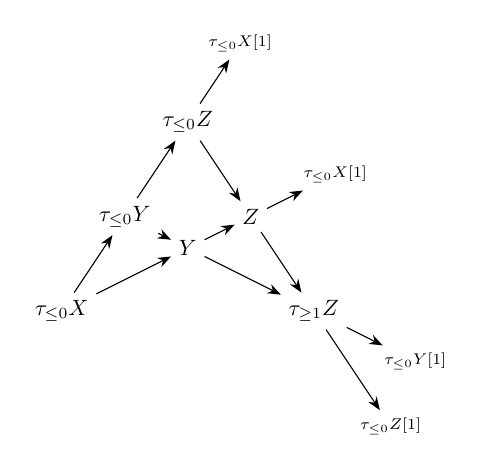
\begin{tikzpicture}[auto, >=Stealth, scale=0.8, transform shape]

  % Define coordinates for nodes
  \node (Z) at (0, 0) {$Y$};
  \node (Y) at (-1, 0.5) {$\tau_{\le 0} Y$};
  \node (X) at (-2, -1) {$\tau_{\le 0} X$};
  \node (Yp) at (1, 0.5) {$Z$};
  \node (Zp) at (0, 2) {$\tau_{\le 0} Z$};
  \node (Xp) at (2, -1) {$\tau_{\ge 1}Z$};
  \node (n1) at (0.83, 3.25) {$\scriptstyle \tau_{\le 0} X[1]$};
  \node (n2) at (2.34, 1.17) {$\scriptstyle \tau_{\le 0} X[1]$};
  \node (n3) at (3.61, -1.80) {$\scriptstyle \tau_{\le 0} Y[1]$};
  \node (n4) at (3.22, -2.83) {$\scriptstyle \tau_{\le 0} Z[1]$};

  % Draw arrows between nodes
  \draw[->] (X) to node[midway, above left] {} (Z);
  \draw[->] (Y) to node[midway, above right] {} (Z);
  \draw[->] (X) to node[midway, below] {} (Y);
  \draw[->] (Z) to node[midway, below] {} (Yp);
  \draw[->] (Z) to node[midway, below] {} (Xp);
  \draw[->] (Y) to node[midway, below] {} (Zp);
  \draw[->] (Zp) to node[midway, below] {} (Yp);
  \draw[->] (Yp) to node[midway, below] {} (Xp);
  \draw[->] (Zp) to node[midway, below] {} (n1);
  \draw[->] (Yp) to node[midway, below] {} (n2);
  \draw[->] (Xp) to node[midway, below] {} (n3);
  \draw[->] (Xp) to node[midway, above] {} (n4);
\end{tikzpicture}
\end{minipage}
\end{center}
we obtain a distinguished triangle \((X, \tau_{\le 0} Y, \tau_{\le 0} Z)\), which is justified by Case 1.

\textbf{Case 2*.} \emph{Dually, if \(Z\) is in \(D^{\ge 0}\), the sequence \(0 \to H^0 X \to H^0 Y \to H^0 Z\) is exact.}

\textbf{General Case.} TR 4 provides an octahedron:

\begin{center}\begin{minipage}{0.45\textwidth}
\centering
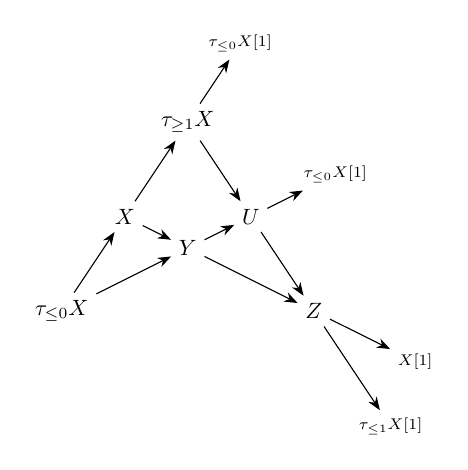
\begin{tikzpicture}[auto, >=Stealth, scale=0.8, transform shape]

  % Define coordinates for nodes
  \node (Z) at (0, 0) {$Y$};
  \node (Y) at (-1, 0.5) {$X$};
  \node (X) at (-2, -1) {$\tau_{\le 0} X$};
  \node (Yp) at (1, 0.5) {$U$};
%% TRANSLATION-FIX: 1.3.6: this vertex is cone(tau_{<=0}X -> X) = tau_{>=1}X
  \node (Zp) at (0, 2) {$\tau_{\ge 1} X$};
%% TRANSLATION-FIX: 1.3.6: this vertex is cone(X -> Y), which is Z by hypothesis
  \node (Xp) at (2, -1) {$Z$};
  \node (n1) at (0.83, 3.25) {$\scriptstyle \tau_{\le 0} X[1]$};
  \node (n2) at (2.34, 1.17) {$\scriptstyle \tau_{\le 0} X[1]$};
  \node (n3) at (3.61, -1.80) {$\scriptstyle X[1]$};
  \node (n4) at (3.22, -2.83) {$\scriptstyle \tau_{\le 1} X[1]$};

  % Draw arrows between nodes
  \draw[->] (X) to node[midway, above left] {} (Z);
  \draw[->] (Y) to node[midway, above right] {} (Z);
  \draw[->] (X) to node[midway, below] {} (Y);
  \draw[->] (Z) to node[midway, below] {} (Yp);
  \draw[->] (Z) to node[midway, below] {} (Xp);
  \draw[->] (Y) to node[midway, below] {} (Zp);
  \draw[->] (Zp) to node[midway, below] {} (Yp);
  \draw[->] (Yp) to node[midway, below] {} (Xp);
  \draw[->] (Zp) to node[midway, below] {} (n1);
  \draw[->] (Yp) to node[midway, below] {} (n2);
  \draw[->] (Xp) to node[midway, below] {} (n3);
  \draw[->] (Xp) to node[midway, above] {} (n4);
\end{tikzpicture}
\end{minipage}
\end{center}
Applying Case 2 to \((\tau_{\le 0} X, Y, U)\) gives an exact sequence: \( H^0 X \to H^0 Y \to H^0 U \to 0. \)
%% TRANSLATION-FIX: 1.3.6: missing comma; the triangle is (U, Z, (tau_{>=1}X)[1])
Case 2*, applied to \((U, Z, (\tau_{\ge 1} X)[1])\), gives: \( 0 \to H^0 U \to H^0 Z \to. \) We deduce the exactness of \(H^0 X \to H^0 Y \to H^0 Z\).

\textbf{Definition.} A \(t\)-structure is \emph{non-degenerate} if the intersection of all \(D^{\leq n}\) and all \(D^{\geq n}\) is reduced to zero objects. For any object \(X\), we write: \( H^i X := H^0(X[i]). \)

\bbdhead{Proposition}{1.3.7}
\emph{If the \(t\)-structure on \(D\) is non-degenerate, the system of functors \(H^i\) is conservative, and for any \(X\) in \(D\) that appears in \(D^{\leq 0}\) (resp. \(D^{\geq 0}\)), it is necessary and sufficient that \(H^i X\) vanishes for \(i > 0\) (resp. for \(i < 0\)).}

%% TRANSLATION-FIX: 1.3.7: for X in D^{<=0}, H^0X = 0 gives X in D^{<=-1}; D^{<=1} is larger and the induction fails
Let \(X\) be in \(D\). We show that if all \(H^i X\) vanish, then \(X = 0\). If \(X\) is in \(D^{\leq 0}\), the assumption \(H^0 X = 0\) ensures that \(X\) is in \(D^{\leq -1}\). Proceeding inductively, we find that \(X\) lies in the intersection of all \(D^{\leq n}\), so \(X = 0\). Dually, if \(X \in D^{\geq 0}\), then \(X = 0\). In the general case, \(\tau_{\leq 0} X\) and \(\tau_{\geq 1} X\) still have their \(H^i\) vanish, so they are zero. Thus, \(X = 0\) by the distinguished triangle \((\tau_{\leq 0} X, X, \tau_{\geq 1} X)\).

If a morphism \(f : X \to Y\), with cone \(Z\), induces isomorphisms \(H^i(X) \overset{\sim}\to H^i(Y)\), the long exact sequence of cohomology shows that \(H^i(Z)\) vanish, so \(Z = 0\), and \(f\) is an isomorphism. Finally, if \(H^i(X)\) vanish for \(i > 0\), then all \(H^i(\tau_{> 0} X)\) vanish, so \(\tau_{> 0} X = 0\), and by (\rn{1.3.4}) \(X \in D^{\leq 0}\). The dual reasoning applies for \(D^{\geq 0}\).

\bbdhead{}{1.3.8}
Theorem \rn{1.3.6}, which associates a \(t\)-structure on \(D\) with an admissible abelian subcategory \(C\) of \(D\), admits a converse stated below (\rn{1.3.9}). The proof will take us to section \rn{1.3.14}. The result will not be used in the rest of these notes.

\bbdhead{}{1.3.9}
Let \(D\) be a triangulated category. Let \(\mathrm{Isom}(D)\) be the set of isomorphism classes of objects of \(D\). For \(X\) in \(D\), let \([X]\) denote its isomorphism class. We define the operation \(*\), which associates two parts of \(\mathrm{Isom}(D)\) with a third:
\[
A * B = \left\{[X] \;\middle|\;
\begin{aligned}
&\text{there exists a distinguished triangle } (U, X, V) \\
&\text{with } [U] \in A \text{ and } [V] \in B
\end{aligned}
\right\}.
\]

\bbdhead{Lemma}{1.3.10}
\emph{The operation \(*\) is associative}

\paragraph{Proof}

It suffices to show that for \(X, Y, Z\) in \(D\),
\[
(([X]) * ([Y])) * ([Z]) = ([X]) * (([Y]) * ([Z])).
\]
For \([T]\) to belong to the left-hand side (resp. the right-hand side), it is necessary and sufficient that \(T\) appears in an upper cap diagram (resp. a lower cap diagram):

\begin{center}
\begin{minipage}{0.45\textwidth}
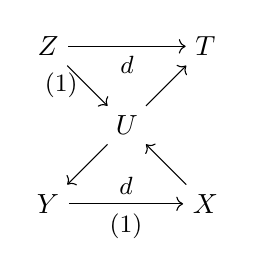
\begin{tikzpicture}
    % Nodes
    \node (Z) at (-1,1) {\(Z\)};
    \node (T) at (1,1) {\(T\)};
    \node (U) at (0,0) {\(U\)};
    \node (Y) at (-1,-1) {\(Y\)};
    \node (X) at (1,-1) {\(X\)};

    % Arrows
    \draw[->] (Z) -- node[below]{\small \(d\)} (T);
    \draw[->] (U) -- node[above right]{} (T);
    \draw[->] (Z) -- node[left]{\small \((1)\)} (U);
    \draw[->] (U) -- node[right]{} (Y);
    \draw[->] (Y) -- node[below]{\small \((1)\)} node[above]{\small \(d\)} (X);
    \draw[->] (X) -- node[below]{} (U);
\end{tikzpicture}
\end{minipage}%
\begin{minipage}{0.45\textwidth}
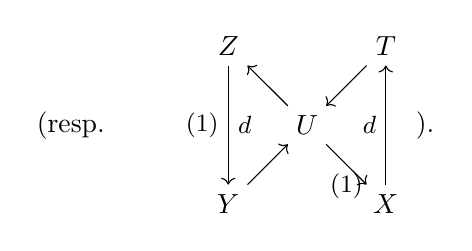
\begin{tikzpicture}
    % Nodes
    \node (Z) at (-1,1) {\(Z\)};
    \node (T) at (1,1) {\(T\)};
    \node (U) at (0,0) {\(U\)};
    \node (Y) at (-1,-1) {\(Y\)};
    \node (X) at (1,-1) {\(X\)};
    \node (cap1) at (-3,0) {\text{(resp.}};
    \node (cap1) at (1.5,-0) {\text{).}};
    % Arrows
    \draw[->] (Z) -- node[right]{\small \(d\)} node[left]{\small \((1)\)} (Y);
    \draw[->] (T) -- node[above right]{} (U);
    \draw[->] (U) -- node[left]{} (Z);
    \draw[->] (Y) -- node[right]{} (U);
    \draw[->] (X) -- node[left]{\small \(d\)} (T);
    \draw[->] (U) -- node[below]{\small \((1)\)} (X);
\end{tikzpicture}
\end{minipage}
\end{center}
The inclusion follows from TR 4, and the reverse inclusion follows from TR 4'.

Lemma \rn{1.3.10} allows us to define the \(*\)-product \(A_1 * \dots * A_p\) of a sequence of subsets of \(\mathrm{Isom}(D)\), without needing to specify how the parentheses are placed. It is convenient to define the \(*\)-product of the empty sequence as \(\{[0]\}\).

\subsection*{\texorpdfstring{\anch{1.3.11}}{1.3.11} Examples}

(i) Let \(A\) be a strictly full subcategory of \(D\), and let \(E A\) be the smallest strictly full subcategory of \(D\) containing \(A\), the zero objects, and stable under extensions. We have:
\[
[E A] = \bigcup_{q \geq 0} [A] * \dots * [A] \quad (q \text{ factors}).
\]

(ii) The statement that every morphism of \(A\) is \(A\)-admissible (\rn{1.2.3}) can be reformulated as:
\[
[A] * [A[1]] \subset [A[1]] * [A].
\]

\bbdhead{}{1.3.12}\footnote{\emph{Errata and Addenda} (2018), item~11: For $I$ the empty interval the definition makes $D^{b,I}$ the empty subcategory; it is more natural to define it as the category of zero objects, so that for every $I$ one has $D^{b,I}=\{A\in D^{b}\mid H^{j}A=0\text{ for }j\notin I\}$.}
Let \(C\) be an admissible abelian subcategory, stable under extensions, of the triangulated category \(D\).

Define \(D^b\) (resp. \(D^{b,\leq 0}\), \(D^{b,\geq 0}\), \(D^{b,I}\), for \(I\) an interval of \(\mathbb{Z}\)) as the smallest strictly full subcategory of \(D\) containing the \(C[n]\) for \(n \in \mathbb{Z}\) (resp. \(-n \leq 0\), \(-n \geq 0\), \(-n \in I\)) and stable under extensions (\rn{1.2.6}).

\bbdhead{Proposition}{1.3.13}
\emph{On \(D^b\), \((D^{b,\leq 0}, D^{b,\geq 0})\) is a non-degenerate \(t\)-structure. For \(a \leq b\), we have \(D^{b,[a,b]} = D^{b,\geq a} \cap D^{b,\leq b}\). In particular, \(C = D^{b,\geq 0} \cap D^{b,\leq 0}\).}

Axiom \rn{1.3.1}(i) of \(t\)-structures follows from the long exact sequence of \(\mathrm{Hom}\) and \rn{1.2.0}. Axiom \rn{1.3.1}(ii) is trivial. Since \(C\) is stable under extensions and satisfies \rn{1.3.11}(ii), for any interval \(I = [a,b]\) of \(\mathbb{Z}\) (\(a \leq b\)), we have:
\[
[D^{b,I}] = [C[-a]] * \dots * [C[-b]].
\]
For \(a \leq c \leq b\), let \(J = [a,c]\) and \(K = [c+1,b]\). Then:
\[
[D^{b,I}] = [D^{b,J}] * [D^{b,K}].
\]

In particular, if \(c = 0\), we find that every object of \(D^{b,I}\) is an extension of an object of \(D^{b,K} \subset D^{b,\geq 1}\) by an object of \(D^{b,J} \subset D^{b,\leq 0}\).

Since \(D^b\) is the increasing union of the \(D^{b,I}\), this proves \rn{1.3.1}(iii).

%% TRANSLATION-FIX: 1.3.13: A_i lies in C[-i], so H^i(X_j) is A_i[i], not A_i[1]
According to (1.3.13.1), if \(X\) is in \(D^{b,I}\), there exists a sequence of distinguished triangles \((X_i, X_{i+1}, A_{i+1})\) (\(a \leq i < b\)) with \(X_a\) in \(C[-a]\), each \(A_j\) in \(C[-j]\), and \(X_b = X\). It is convenient to set \(X_{a-1} = 0\), and to complete this sequence with an initial triangle \((X_{a-1}, X_a, A_a) = (0, X_a, X_a)\). Applying the long exact sequence of cohomology to these triangles, we prove by induction on \(j\) that, for all \(i\), \(H^i(X_j)\) is 0 for \(i \notin [a,j]\) and is \(A_i[i]\) for \(i \in [a,j]\). In particular:
\[
[X] \in \{[H^a(X)[-a]] * \dots * [H^b(X)[-b]]\}.
\]
\(X\) is a successive extension of its cohomology objects, placed in their respective degrees. From this follows the non-degeneracy of the \(t\)-structure (if the \(H^i X\) vanish, then \(X\) is zero) and the second statement of \rn{1.3.13} (if \(X\) is in \(D^{b,\geq a} \cap D^{b,\leq b}\), its \(H^i X\) vanish for \(i \notin [a,b]\), and hence \(X\) is in \(D^{b,[a,b]}\)).

\bbdhead{Remark}{1.3.14}
Let \(D\) be a triangulated category, and \(C\) a full subcategory satisfying \rn{1.2.0}, where every morphism is admissible. The proof of \rn{1.2.4} shows that every morphism in \(C\) has a kernel and a cokernel, that \(\mathrm{Im}(f) = \mathrm{Coim}(f)\), and that every short exact sequence in \(C\) is admissible. For \(C\) to be abelian, it only lacks the existence of finite direct sums.

Let \(C'\) be the category \(EC\) of successive extensions of objects in \(C\) (\rn{1.3.11}(i)). The exact sequence of \(\mathrm{Hom}\) shows that \(C'\) still satisfies (\rn{1.2.0}). Moreover, from (1.3.11.1) and (1.3.11.2) applied to \(C\), and from the associativity of \(*\), it follows that \([C'] * [C'[1]] \subset [C'[1]] * [C']\), i.e., every morphism in \(C'\) is admissible: \(C'\) is an admissible abelian subcategory of \(D\). Applying \rn{1.3.13} to \(C'\), we deduce that, for \(D^b\), \(D^{b,\geq 0}\) and \(D^{b,\leq 0}\) as defined in \rn{1.3.12} (based on \(C\)), \((D^{b,\leq 0}, D^{b,\geq 0})\) forms a \(t\)-structure on \(D^b\), with heart \(C'\).

The following proposition provides intermediaries between the functors \(\tau_{\leq 0}\) and \(\tau_{<0}\).

\bbdhead{Proposition}{1.3.15}
\emph{Let \(K\) be in \(D\) and suppose there is a short exact sequence in \(C\):}
\[
0 \to A \to H^0 K \to B \to 0.
\]

\emph{(i) There exists \(K'\) in \(D^{\leq 0}\), equipped with \(a : K' \to K\), such that for all \(L\) in \(D^{\leq 0}\), \(a\) identifies \(\mathrm{Hom}(L, K')\) with the subgroup of \(\mathrm{Hom}(L, K)\) formed by morphisms \(f\) such that \(H^0(f)\) factors through \(A\). In other words, in \(D^{\leq 0}\), \(K'\) corepresents the functor \(L \mapsto \ker(\mathrm{Hom}(L, K) \to \mathrm{Hom}(H^0(L), B))\). For a pair \((K', a)\) to corepresent this functor, it is necessary and sufficient that:}
\[
(*) K' \in D^{\leq 0}, \quad \tau_{<0} K' \to \tau_{<0} K \quad \text{and} \quad H^0 K' \to A \subset H^0 K.
\]

\emph{(ii) Dually, there exists \(b : K \to K''\) with \(K'' \in D^{\geq 0}\) and, for \(L\) in \(D^{\geq 0}\), a short exact sequence:}
\[
0 \to \mathrm{Hom}(K'', L) \to \mathrm{Hom}(K, L) \to \mathrm{Hom}(A, H^0 L).
\]

\emph{The pair \((K'', b)\) is characterized by \(K'' \in D^{\geq 0}\), \(\tau_{>0} K \to \tau_{>0} K''\), and \(H^0 K'' = B\).}

%% TRANSLATION-FIX: 1.3.15(iii): the morphism supplied is the closing degree-1 arrow K'' -> K'[1]
\emph{(iii) There exists \(d : K'' \to K'[1]\), unique by \rn{1.1.10}, such that \((K', K, K'')\) forms a distinguished triangle.}

Let the morphism \(\tau_{\le 0} K \to H^0 K \to B\) and \(K'\) complete the distinguished triangle \((K', \tau_{\le 0} K, B)\). This triangle shows that \(K'\) is in \(D^{\leq 1}\) and that \(H^1 K' = 0\), so \(K'\) is in \(D^{\le 0}\). For \(L\) in \(D^{\le 0}\), we have \(\mathrm{Hom}^{-1}(L, B) = 0\), leading to the exact sequence:
\[
0 \to \mathrm{Hom}(L, K') \to \mathrm{Hom}(L, \tau_{\le 0} K) \to \mathrm{Hom}(L, B).
\]
With \(\mathrm{Hom}(L, \tau_{\le 0} K) \overset{\sim}\to \mathrm{Hom}(L, K)\) and \(\mathrm{Hom}(L, B) = \mathrm{Hom}(H^0 L, B)\), the sequence becomes:
\[
0 \to \mathrm{Hom}(L, K') \to \mathrm{Hom}(L, K) \to \mathrm{Hom}(H^0 L, B),
\]
%% TRANSLATION-FIX: 1.3.15: the triangle constructed above is (K', tau_{<=0}K, B)
%% ERRATUM 12
showing that \(K'\) represents functor (i). For \(L\) in \(D^{<0}\), the universal property of \(K'\) shows that \(\tau_{<0} K' \to \tau_{<0} K\). The long exact sequence of cohomology of \((K', \tau_{\le 0} K, B)\) shows that \(H^0 K'\overset{\sim} \to A\). Conversely, if \(K_1'\) satisfies (*), the universal property of \(K'\) provides a morphism \(a : K_1' \to K'\), which induces the isomorphisms \(\tau_{<0} K_1' \to \tau_{<0} K'\) and \(H^0 K_1' \to H^0 K'\). The morphism \(a\) is therefore an isomorphism, completing the proof of (i). The assertion (ii) is obtained by duality.

Let us construct an octahedron on \(K' \to \tau_{\le 0} K \to K\):

\begin{center}\begin{minipage}{0.45\textwidth}
\centering
\begin{tikzpicture}[auto, >=Stealth, scale=0.8, transform shape]

  % Define coordinates for nodes
  \node (Z) at (0, 0) {$K$};
  \node (Y) at (-1, 0.5) {$\tau_{\le 0} K$};
  \node (X) at (-2, -1) {$K'$};
  \node (Yp) at (1, 0.5) {$K_1''$};
  \node (Zp) at (0, 2) {$B$};
  \node (Xp) at (2, -1) {$\tau_{>0}K$};
  \node (n1) at (0.83, 3.25) {$\scriptstyle K'[1]$};
  \node (n2) at (2.34, 1.17) {$\scriptstyle K'[1]$};
  \node (n3) at (3.61, -1.80) {$\scriptstyle \tau_{\le 0} K[1]$};
  \node (n4) at (3.22, -2.83) {$\scriptstyle B[1]$};

  % Draw arrows between nodes
  \draw[->] (X) to node[midway, above left] {} (Z);
  \draw[->] (Y) to node[midway, above right] {} (Z);
  \draw[->] (X) to node[midway, below] {} (Y);
  \draw[->] (Z) to node[midway, below] {} (Yp);
  \draw[->] (Z) to node[midway, below] {} (Xp);
  \draw[->] (Y) to node[midway, below] {} (Zp);
  \draw[->] (Zp) to node[midway, below] {} (Yp);
  \draw[->] (Yp) to node[midway, below] {} (Xp);
  \draw[->] (Zp) to node[midway, below] {} (n1);
  \draw[->] (Yp) to node[midway, below] {} (n2);
  \draw[->] (Xp) to node[midway, below] {} (n3);
  \draw[->] (Xp) to node[midway, above] {} (n4);
\end{tikzpicture}
\end{minipage}
\end{center}

The triangle \((B, K_1'', \tau_{>0} K)\) is of the type \rn{1.3.1}(iii) for \(K_1''\). It shows that \(K_1''\) is in \(D^{\geq 0}\), with \(H^0 K'' = B\) and \(\tau_{>0} K \overset{\sim}\to \tau_{>0} K_1''\). By (ii), \(K''_1\) identifies with \(K''\), and \((K', K, K_1'')\) is the triangle promised in (iii).

\bbdhead{}{1.3.16}
Let \(D_i\) (\(i = 1, 2\)) be two \(t\)-categories, \(C_1\) the heart of \(D_1\), and let \(\epsilon\) be the inclusion functor of \(C_1\) into \(D_1\). Let \(T : D_1 \to D_2\) be an exact functor (\cite{Verdier}, p.4) from the triangulated category \(D_1\) to the triangulated category \(D_2\). We say \(T\) is \(t\)-exact on the right if \(T(D^{\leq 0}_1) \subset D^{\leq 0}_2\), \(t\)-exact on the left if \(T(D^{\geq 0}_1) \subset D^{\geq 0}_2\), and \(t\)-exact if it is \(t\)-exact on both the left and the right.

\bbdhead{Proposition}{1.3.17}
%% ERRATUM 13
\emph{(i) If \(T\) is \(t\)-exact on the left (resp. on the right), the additive functor \({}^p T := H^0 \circ T \circ \epsilon : C_1 \to C_2\) is exact on the left (resp. on the right).}

\emph{(ii) For \(T\) \(t\)-exact on the left (resp. on the right) and \(K \in D^{\geq 0}_1\) (resp. \(K \in D^{\leq 0}_1\)), we have:}
\[
{}^pT H^0( K) \to H^0( T K) \quad (\text{resp. } H^0 (T K) \to {}^pT H^0 (K)).
\]

\emph{(iii) Let \((T^*, T_*)\) be a pair of exact adjoint functors:
\[
T^* : D_2 \to D_1, \quad T_* : D_1 \to D_2,
\]
%% TRANSLATION-FIX: 1.3.17(iii): T^* is the LEFT adjoint of T_*, as the proof below uses
where \(T^*\) is the left adjoint of \(T_*\). For \(T^*\) to be \(t\)-exact on the right, it is necessary and sufficient that \(T_*\) be \(t\)-exact on the left. In this case, \(({}^pT^*, {}^pT_*)\) forms a pair of adjoint functors between \(C_1 \leftrightarrow C_2\).}

%% TRANSLATION-FIX: 1.3.17(iv): a one-sided hypothesis gives only a one-sided conclusion
\emph{(iv) If \(T_1 : D_1 \to D_2\) and \(T_2 : D_2 \to D_3\) are \(t\)-exact on the left (resp. on the right), then \(T_2 \circ T_1\) is also \(t\)-exact on the left (resp. on the right), and:}
\[
{}^p(T_2 \circ T_1) = {}^p{T_2} \circ{}^p{T_1}.
\]

If \(T\) is \(t\)-exact on the left, for any short exact sequence \(0 \to X \to Y \to Z \to 0\) in \(C_1\), the long exact sequence of cohomology for the distinguished triangle \((T(X), T(Y), T(Z))\) provides:
\[
0 \to H^0 T(X) \to H^0 T(Y) \to H^0 T(Z),
\]
as \(T(Z) \in D_2^{\geq 0}\). This (resp. the dual statement) proves (i).

For \(K \in D_1^{\geq 0}\), the triangle \((H^0 K, K, \tau_{>0} K)\) provides a distinguished triangle: \( (TH^0 K, T(K), T\tau_{>0} K), \)
%% TRANSLATION-FIX: 1.3.17(ii): tau_{>0}K lives in D_1; it is T tau_{>0}K that lies in D_2^{>0}
where \(T\tau_{>0} K \in D_2^{>0}\). The long exact sequence of cohomology then provides: \( H^0 T(H^0 K) \overset{\sim}\to H^0 T(K) .\) This (resp. the dual statement) proves (ii).

If \(T_*\) is \(t\)-exact on the left, for \(U \in D_1^{>0}\) and \(V \in D_2^{\le 0}\), we have: \( \mathrm{Hom}(T^* V, U) = \mathrm{Hom}(V, T_* U) = 0. \)
%% TRANSLATION-FIX: 1.3.17(iii): T^*B lies in D_1^{<=0}, so H^0 T^*B = tau_{>=0}T^*B
This holds for all \(U\), so \(\tau_{>0} T^* V = 0\), i.e., \(T^* V \in D_1^{\leq 0}\). Hence \(T^*\) is \(t\)-exact on the right. For \(A \in C_1\) and \(B \in C_2\), we then have \(H^0 T^* B = \tau_{\ge 0}T^* B\) and \(H^0 T_* A = \tau_{\le 0}T_* A\) where the functorial isomorphism:
\[
\begin{aligned}
\mathrm{Hom}(H^0 T^* B, A) &\overset{\sim}\to \mathrm{Hom}(T^* B, A) \\
&= \mathrm{Hom}(A, T_* B) \overset{\sim}\leftarrow \mathrm{Hom}(A, H^0 T_* B)
\end{aligned}
\]
Thus, together with duality completing the proof of (iii).

If \(T_1\) and \(T_2\) are \(t\)-exact on the left, and \(A \in C_1\), with \(T_1 A_1\in D^{\ge 0}\) then: \( {}^p(T_2 \circ T_1) A = H^0 T_2 T_1 A = H^0 T_2 H^0 {T_1} A. \) by (ii). This, completed by duality, proves (iv).

\bbdhead{Remark}{1.3.18}
(i) Let \(D_1^{+} = \bigcup_{n \geq 0} D_1^{\geq -n}\) and \(D_2^{-} = \bigcup_{n \geq 0} D_2^{\leq n}\). The result (iii) still holds for \(T^* : D_2^- \to D_1\) and \(T_* : D_1^+ \to D_2\), adjoint in the sense that:
\[
\mathrm{Hom}(T^* V, U) = \mathrm{Hom}(V, T_* U), \quad \text{for } V \in D_2^{-}, \, U \in D_1^{+}.
\]
The proof is the same.

(ii) For \(A \in C_1\) and \(B \in C_2\), the adjunction arrows for \((T^*, T_*)\) and \(({}^pT^*, {}^pT_*)\) are linked by the following commutative diagrams:
\[
\begin{tikzcd}
T^{*}{}^{p}T_* A \arrow[r] \arrow[d] &{ }^{p}T^{*}{}^{p}T_* A  \arrow[d] \\
T^* T_* A \arrow[r] & A
\end{tikzcd}
\quad
\begin{tikzcd}
%% TRANSLATION-FIX: 1.3.18(ii): the adjunction unit is B -> T_*T^*B; T^*T_*B is not defined for B in C_2
B \arrow[r] \arrow[d] & T_*T^*B \arrow[d] \\
{ }^{p}T_{*}^{p}T^*B  \arrow[r] & T_{*}^{p}T^*B
\end{tikzcd}.
\]
\bbdhead{}{1.3.19}
Let \(T : D' \to D\) be an exact fully faithful functor between triangulated categories. For a triangle \(tr\) in \(D'\) to be distinguished, it suffices that its image \(T(tr)\) under \(T\) be so: if \(tr_1\) is a distinguished triangle with the same base as \(tr\), then \(T(tr)\) and \(T(tr_1)\) are distinguished with the same base, hence isomorphic, and \(tr\) and \(tr_1\) are isomorphic.

Suppose \(D\) and \(D'\) are equipped with \(t\)-structures, and let \(T\) be \(t\)-exact. For \(X\) in \(D'\), \(X \in D'^{\leq 0}\) (resp. \(X \in D'^{\geq 0}\)) if and only if \(T(X) \in D^{\leq 0}\) (resp. \(T(X) \in D^{\geq 0}\)): for \(X \in D'^{\leq 0}\) \(\Leftrightarrow\tau_{> 0} X = 0\), and \(T\) commutes with \(\tau_{> 0}\) (resp. dual argument).

%% TRANSLATION-FIX: 1.3.19: the induced t-structure is a structure on D', not on D
Conversely, if \(D'\) is a full triangulated subcategory of a triangulated category \(D\), and \((D^{\leq 0}, D^{\geq 0})\) is a \(t\)-structure on \(D\), for \((D'^{\leq 0}, D'^{\geq 0}) := (D'\cap D^{\leq 0}, D'\cap D^{\geq 0})\), to be a \(t\)-structure on \(D'\), it is necessary and sufficient that \(D'\) be stable under the functor \(\tau_{\leq 0}\). If this condition is met, this \(t\)-structure on \(D'\) is called the \emph{induced \(t\)-structure}. For \(D'\) equipped with the induced \(t\)-structure, the inclusion functor of \(D'\) in \(D\) is \(t\)-exact: we have $C'=D'\cap C$, and the restriction to \(D'\) of the functor \(\tau_{\leq p}\), \(\tau_{\geq p}\), or \(H^0\) of \(D\) coincides with the functor of the same name on \(D'\).

\bbdhead{}{1.3.20}
Let \((D_i)_{i \in I}\) be a finite family of triangulated categories and \(T : \prod_{i \in I} D_i \to D\) be an exact multifunctor (SGA 4 XVIII \rn{1.1.3}) from the \(D_i\) into a triangulated category \(D\). Suppose the \(D_i\) are equipped with \(t\)-structures. We say \(T\) is \(t\)-exact on the left (resp. on the right) if it maps the product of \(D_i^{\geq 0}\) (resp. \(D_i^{\leq 0}\)) into \(D^{\geq 0}\) (resp. \(D^{\leq 0}\)), and \(t\)-exact if it is \(t\)-exact on both sides. If \(T\) is \(t\)-exact on the left (resp. on the right) and certain variables are fixed to an object given in \(D_i^{\geq 0}\) (resp. \(D_i^{\leq 0}\), resp. \(C_i\), the heart of \(D_i\)), the functor obtained in the remaining variables is still \(t\)-exact on the left (resp. on the right, resp. in both directions). This allows us to apply \(T\) to results proven for functors in one variable. For example:

Let \(\epsilon_i\) denote the inclusion of \(C_i\) into \(D_i\). Define:
\[
{}^pT := H^0 \circ T \circ (\epsilon_i)_{i \in I}.
\]
If \(T\) is \(t\)-exact on the left (resp. on the right), the additive multifunctor \({}^pT\) from \((C_i)_{i \in I}\) into \(C\) is exact on the left (resp. on the right).

Suppose \(T\) is \(t\)-exact on the left. For the \(K_i \in D_i^{\geq 0}\), we have By \rn{1.3.17}(ii),
\[
{}^pT(H^0 K_i) \to H^0 T(K_i),
\]
for any \(K_i\), the morphism \(K_i \to \tau_{\ge 0} K_i\) provides a morphism:
\[
H^0 T(K_i) \to H^0 T(\tau_{\ge 0} K_i) \overset{\sim}\leftarrow {}^pT(H^0 K_i) \eqtag{1.3.20.1}.
\]
By translation, more generally, for \(\sum n_i= n\), we obtain a morphism:
\[
H^n T(K_i) \to {}^pT(H^{n_i} K_i) \eqtag{1.3.20.2}.
\]
There is a sign issue, which does not arise if we consider instead:
\[
H^n T(K_i) \to H^n T((H^{n_i} K_i)[-n_i]) \eqtag{1.3.20.3}.
\]

For \(T\) \(t\)-exact on the right, we have \({}^p T H^0 K_i \overset{\sim}\leftarrow H^0 T(K_i)\) for \(K_i \in D_i^{\le 0}\); the morphisms \(\tau_{\le 0} K_i \to K_i\) provide a morphism: \( {}^p T(H^0 K_i) \to H^0 T(K_i), \) and, by translation, morphisms:
\[
H^n T((H^n_i K_i)[-n_i]) \to H^n T(K_i) \quad (\mbox{with }\sum n_i=n)\eqtag{1.3.20.4}.
\]

For \(T\) \(t\)-exact, we have both (\rn{1.3.20.3}) and (\rn{1.3.20.4}). Applying \(H^n T\) to the commutative diagrams:
\[
\begin{tikzcd}
\tau_{\leq n_i} K_i \arrow[r] \arrow[d] & H^{n_i} K_i[-n_i] \arrow[d] \\
K_i \arrow[r] & \tau_{\ge n_i} K_i
\end{tikzcd},
\]
we find that the composite of (\rn{1.3.20.3}) and (\rn{1.3.20.4}) is the identity. If \(\sum n_i = \sum m_i = n\) and \((n_i)_{i \in I} \neq (m_i)_{i \in I}\), there exists \(i\) such that \(n_i < m_i\). The composite: \( \tau_{\leq n_i} K_i \to K_i \to \tau_{\geq m_i} K_i \) vanishes, and we deduce that the composite \(((1.3.20.3)\mbox{ for (}n_i\mbox{) )} \circ ((1.3.20.4)\mbox{ for (}m_i\mbox{) )}\) vanishes.

\bbdhead{Proposition}{1.3.21}
\emph{If \(T\) is \(t\)-exact and the \(K_i\) are in \(D_i^b\), the morphisms (\rn{1.3.20.3}) and (\rn{1.3.20.4}) define inverse isomorphisms to each other:}
\[
H^n T(K_i) = \bigoplus H^n T((H^{n_i} K_i)[-n_i]) \quad \text{(sum over \(\Sigma n_i = n\))} \eqtag{1.3.21.1}.
\]

We have already seen that these morphisms make the second term a direct summand of the first. Both terms in \rn{1.3.21.1} are cohomological functors on each \(K_i\) (for the right-hand term, due to the exactness of \({}^pT\)), and the morphisms (\rn{1.3.20.3}) and (\rn{1.3.20.4}) are morphisms of cohomological functors. By induction, we reduce to the case where each \(K_i \in C_i\); this case is trivial.

\subsection*{\texorpdfstring{\anch{1.3.22}}{1.3.22} Examples of $t$-structures}
(This will not be used later in these notes.)

Let $\mathcal{A}$, as in \rn{1.1.4}, be an exact category, with a set of short exact sequences $\mathcal{E}$. Suppose that every morphism $f: A \to B$ admits a kernel such that $\ker(f) \to A$ fits into a short exact sequence
\[
0 \to \ker(f) \to A \to \mathrm{Coim}(f) \to 0.
\]
Let $\mathcal{D}^{\le 0}$ (resp. $\mathcal{D}^{\ge 0}$) denote the subcategory of $\mathcal{D} = D(\mathcal{A})$ (\rn{1.1.4}) consisting of complexes $K$ such that the morphisms \( \mathrm{Coim}(d^{i-1}) \to \ker(d^i) \)
%% TRANSLATION-FIX: 1.3.22: D^{>=0} is H^i = 0 for i < 0; i <= 0 would define D^{>=1}
are isomorphisms for $i > 0$ (resp. $i < 0$).

In terms of the embedding $h : \mathcal{A} \to (\mathcal{A}, \mathcal{E})$ (\rn{1.1.4}), this means that the image $h_K$ of $K$ in $(\mathcal{A}, \mathcal{E})^\tau$ belongs to $\mathcal{D}^{\le 0}$ (resp. $\mathcal{D}^{\ge 0}$). We show that $(\mathcal{D}^{\le 0}, \mathcal{D}^{\ge 0})$ forms a $t$-structure on $\mathcal{D}$.

(a) For $K, L$ in $\mathcal{D}$:
    \[\mathrm{Hom}_\mathcal{D}(K, L) = \varinjlim \mathrm{Hom}_{K\mathcal{A}}(K', L'),
    \]
where the limit is taken over homotopy classes of quasi-isomorphisms $K' \to K$ and $L \to L'$. For $K$ in $\mathcal{D}^{\le 0}$ (resp. $L$ in $\mathcal{D}^{\ge 1}$), a cofinal system of $K'$ (resp. $L'$) is obtained by restricting to those such that $K'^i = 0$ for $i > 0$ (resp. $L'^i = 0$ for $i < 0$). Use the quasi-isomorphism $\tau_{\le 0}K' \to K'$ (resp. $\tau_{\ge 1}L' \to L'$), where $\tau_{\le 0}$ and $\tau_{\ge 1}$ are as in \rn{1.3.2}(i).

For such $K'$ and $L'$, any morphism of complexes $f: K' \to L'$ vanishes: it is defined by $f^0: K'^0 \to L'^0$, satisfying $df^0 = 0$, and thus vanishes because $d: L'^0 \to L'^1$ is a monomorphism. This verifies \rn{1.3.1}(i). The axiom \rn{1.3.1}(ii) is trivial.

(b)For $K$ in $K\mathcal{A}$, there exists a short exact sequence of complexes
    \[
    0 \to \tau_{\le 0}K \to K \to \tau_{\ge 1}K \to 0.
    \]
This defines a distinguished triangle in $\mathcal{D}$: the cone of $\tau_{\le 0}K \to K$ maps quasi-isomorphically to $\tau_{\ge 1}K$. This verifies \rn{1.3.1}(iii).

In particular, the heart $\mathcal{C}$ of $\mathcal{D}$ is an abelian category. The objects of $\mathcal{C}$ can be represented as complexes $K$ of length 1: \( K = K^{-1} \to K^0, \) where $d$ is a monomorphism. For $K$ and $L$ of this type, a morphism of complexes $f: K \to L$ is uniquely determined by its component $f^0: K^0 \to L^0$. Identifying $K^{-1}$ and $L^{-1}$ as subobjects of $K^0$ and $L^0$, respectively, $f^0: K^0 \to L^0$ arises from a morphism of complexes $f$ if and only if $f^0(K^{-1}) \subseteq L^{-1}$. Moreover, $f$ is homotopic to zero if and only if $f^0(K^0) \subseteq L^{-1}$. That $f$ is a quasi-isomorphism means the exactness of
\[
0 \to K^{-1} \to K^0 \oplus L^{-1} \to L^0 \to 0,
\]
i.e., that $K^0 \oplus L^{-1} \to L^0$ is an admissible epimorphism, and that the subobject $K^{-1}$ of $K^0$ is the pull-back of $L^{-1}$ by $f^0$.

It is easily verified that if $K' \overset{\varphi}\to K$ is a quasi-isomorphism, (concentrated in degrees $0$ and $-1$), and $f\varphi$ is homotopic to zero ($f\varphi(K^0) \subseteq L^{-1}$), then $f$ is also homotopic to zero. The group $\mathrm{Hom}_{\mathcal{C}}(K, L)$ is the inductive limit, for $\varphi : K' \to K$ a quasi-isomorphism of this type, of
\[
\mathrm{Hom}_{K\mathcal{A}}(K', L) =
\frac{\{f : K'^0 \to L^0 \mid f(K'^{-1}) \subseteq L^{-1}\}}
     {\{f \mid f(K'^0) \subseteq L^{-1}\}}.
\]
and, in this inductive limit, the transition morphisms are injective.

\subsection*{\texorpdfstring{\anch{1.3.23}}{1.3.23} Exercises}
\textbf{(i)} For $K$ a complex of objects in $\mathcal{A}$, $H^0K$ in $\mathcal{C}$ is the complex $\mathrm{Coim}(d^{-1}) \to \ker(d^0)$.

\textbf{(ii)} A functor $F$ from $\mathcal{A}$ to an abelian category $\mathcal{N}$ that transforms sequences in $\mathcal{E}$ into right exact sequences $FA \to FB \to FC \to 0$ extends uniquely (up to unique isomorphism) to $F' : \mathcal{C} \to \mathcal{N}$, which is right exact. If $F$ is fully faithful and transforms sequences in $\mathcal{E}$ into short exact sequences and monomorphisms into monomorphisms, then $F'$ is exact and fully faithful. In particular, the composite functor
\[
\mathcal{C} \rightarrow D\mathcal{A}\rightarrow D((\mathcal{A},\mathcal{E})^{\sim})\overset{H^0}{\to} (\mathcal{A},\mathcal{E})^{\sim}
\]
is fully faithful. It identifies $\mathcal{C}$ with the category of quotients in $(\mathcal{A}, \mathcal{E})$ of an object of $\mathcal{A}$ by a subobject in $\mathcal{A}$.

\textbf{(iii)} The functor $D^-\mathcal{A} \to D^-\mathcal{C}$ (the superscript $-$ indicates that we restrict to bounded above complexes) is an equivalence [use the fact that every object in $\mathcal{C}$ is a quotient of an object in $\mathcal{A}$].

\textbf{(iv)} Let $\mathcal{A}$ be an abelian category. The hypotheses of \rn{1.3.22} are satisfied by $F\mathcal{A}$ (\rn{1.1.3} example 2). Let $\mathcal{C}$ be the corresponding abelian category of formal quotients of filtered objects, and let $\mathcal{C}'$ be the category of sequences
\[
\dots \to A^i \to A^{i-1} \to \dots
\]
with $A^i = 0$ for $i \gg 0$ and $A^i \to A^{i-1}$ for $i \ll 0$. Show that the functor $((V^{-1}, F) \to (V^0, F)) \mapsto (\mathrm{coker}(F^{-1} \to F^0))$ from $\mathcal{C}$ to $\mathcal{C}'$ is an equivalence [apply (ii)].

\subsection*{\texorpdfstring{\anch{1.3.24}}{1.3.24} Example}
The hypotheses of \rn{1.3.22} are satisfied for $\mathcal{A}$, the category of Banach spaces, if we take as short exact sequences those that become exact after forgetting the topology, i.e., by the closed graph theorem, the sequences isomorphic to
\[
0 \to A \to B \to C \to 0,
\]
where $A$ is a closed subspace of $B$ and $C = B/A$. The category $\mathcal{C}$ obtained is a category of "formal quotients" $B/A$ (for $A \to B$ a continuous injective linear map between Banach spaces). The closed graph theorem ensures that if the complexes $K^{-1} \to K^0$ and $L^{-1} \to L^0$ define objects in $\mathcal{C}$, a morphism of complexes $f: K \to L$ corresponds to a continuous linear map $f^0: K^0 \to L^0$ such that set-theoretically $f(K^{-1}) \subseteq L^{-1}$, and $f$ is homotopic to zero (i.e., null in $\mathcal{C}$) if and only if, set-theoretically, $f(K^0) \subseteq L^{-1}$.

%% ERRATUM 16
Similar formal quotients have been considered by L.~Waelbroeck \cite{Wae72}.

\section{Gluing}

\bbdhead{}{1.4.1}
For $X$ a topological space (or a topos) equipped with a sheaf of rings $\mathcal{O}$, we denote by $\mathcal{D}(X, \mathcal{O})$ the derived category of the abelian category $\mathcal{M}(X, \mathcal{O})$ of sheaves of $\mathcal{O}$-modules on $X$. As usual, $\mathcal{D}^+(X, \mathcal{O})$ is the full subcategory of bounded below complexes in $\mathcal{D}(X, \mathcal{O})$.

Let $U$ be an open subset of $X$, $F$ the complementary closed subset, $j$ the inclusion of $U$ into $X$, and $i$ the inclusion of $F$ into $X$. We also denote by $i^*$ the inverse image of $\mathcal{O}$ on $U$ or $F$. We aim to describe a construction that attaches a $t$-structure on $\mathcal{D}^+(U, \mathcal{O})$ and one on $\mathcal{D}^+(F, \mathcal{O})$ to a $t$-structure on $\mathcal{D}^+(X, \mathcal{O})$.

The categories $\mathcal{M}(X, \mathcal{O})$, $\mathcal{M}(U, \mathcal{O})$, and $\mathcal{M}(F, \mathcal{O})$ are connected by the functors:
\[
\begin{aligned}
%% TRANSLATION-FIX: 1.4.1: extension by zero is j_!, not j_*
j_!  & : \mathcal{M}(U, \mathcal{O}) \to \mathcal{M}(X, \mathcal{O})
\quad & \text{extension by \(0\),} & \text{(exact)}; \\
j^*  & : \mathcal{M}(X, \mathcal{O}) \to \mathcal{M}(U, \mathcal{O})
\quad & \text{restriction, also denoted \(j^!\),} & \text{(exact)}; \\
%% TRANSLATION-FIX: 1.4.1: the direct image is j_*, not j_!
j_*  & : \mathcal{M}(U, \mathcal{O}) \to \mathcal{M}(X, \mathcal{O})
\quad & \text{direct image,} & \text{(left exact)}; \\
i^*  & : \mathcal{M}(X, \mathcal{O}) \to \mathcal{M}(F, \mathcal{O})
\quad & \text{restriction,} & \text{(exact)}; \\
i_*  & : \mathcal{M}(F, \mathcal{O}) \to \mathcal{M}(X, \mathcal{O})
\quad & \text{direct image, also denoted \(i_!\),} & \text{(exact)}; \\
i^!  & : \mathcal{M}(X, \mathcal{O}) \to \mathcal{M}(F, \mathcal{O})
\quad & \text{sections with support in \(F\),} & \text{(left exact)}.
\end{aligned}
\]
%% TRANSLATION-FIX: 1.4.1: j^*j_* = id; the vanishing composite is j^*i_* = 0, whence i^*j_! = 0
These form two sequences of three adjoint functors $(j_!, j^*, j_*)$ and $(i^*, i_*, i^!)$. We have $j^* i_* = 0$, hence by adjunction $i^! j_* = 0$ and $i^* j_! = 0$. For any sheaf $F$ on $X$, the adjunction arrows give exact sequences:
\[
0 \to j_! j^* F \to F \to i_* i^* F \to 0 \eqtag{1.4.1.1}
\]
and
\[
%% TRANSLATION-FIX: 1.4.1: this sequence is only left exact, and the tag belongs to the isomorphism below
0 \to i_* i^! F \to F \to j_* j^* F
\]
(which can be completed by $0$ on the right for $F$ injective).

For $F$ on $F$ (resp. $U$), they provide the isomorphisms:
\[
%% TRANSLATION-FIX: 1.4.1.2: the composites are reversed; these are the counit i^*i_* and the unit i^!i_*
i^* i_* F \to F \to i^! i_* F, \eqtag{1.4.1.2}
\]
\[
%% TRANSLATION-FIX: 1.4.1.3: same reversal on the open side
j^* j_! F \to F \to j^* j_* F. \eqtag{1.4.1.3}
\]

%% TRANSLATION-FIX: 1.4.2: with T^* left adjoint to T_*, the counit is T^*T_* -> Id and the unit Id -> T_*T^*
%% TRANSLATION-FIX: 1.4.2: j^* is a localization and is never fully faithful
For any pair of adjoint functors $(T^*, T_*)$, the adjunction morphism $T^* T_* \to \mathrm{Id}$ (resp. $\mathrm{Id} \to T_* T^*$) is an isomorphism if and only if $T_*$ (resp. $T^*$) is fully faithful. Assertions (\rn{1.4.1.2}) and (\rn{1.4.1.3}) imply that $i_*$, $j_!$, and $j_*$ are fully faithful.

\bbdhead{}{1.4.2}
When a functor $T$ between abelian categories is exact, it trivially extends to derived categories. We will often denote
\[
T : \mathcal{D}^+(X, \mathcal{O}) \to \mathcal{D}^+(X, \mathcal{O}).
\]by the same symbol for the functor and its extension to derived categories. This extension is both the left derived functor $LT$ and the right derived functor $RT$ of $T$.

\num{\anch{1.4.2.1}.}
The functors of \rn{1.4.1} provide by derivation (on the right) functors linking $\mathcal{D}^+(X, \mathcal{O})$, $\mathcal{D}^+(U, \mathcal{O})$, and $\mathcal{D}^+(F, \mathcal{O})$, forming two sequences of three adjoint functors $(j_!, j^*, Rj_*)$ and $(i^*, i_*, Ri^!)$. We have $j^* i_* = 0$, hence by adjunction $i^*j_!=0$ and $Ri^! j_* = 0$. For every $K$ in $\mathcal{K}^+(X, \mathcal{O})$, the sequences (\rn{1.4.1.1}) give rise to distinguished triangles:
\[
(j_! j^* K, K, i_* i^* K) \quad \text{and} \quad (i_* Ri^! K, K, Rj_* j^* K).
\]
For $K$ in $\mathcal{D}^+(F, \mathcal{O})$ (resp. $\mathcal{D}^+(U, \mathcal{O})$), (\rn{1.4.1.2}) (resp. \rn{1.4.1.3}) provides the isomorphisms:
\[
%% TRANSLATION-FIX: 1.4.2.1: derived form of (1.4.1.2); as printed the arrows do not typecheck
i^* i_* K \to K \to Ri^! i_* K \quad \text{(where $i_*$ is fully faithful)}
\]

\[
%% TRANSLATION-FIX: 1.4.2.1: derived form of (1.4.1.3); as printed the arrows do not typecheck
\text{(resp. }j^* j_! K \to K \to j^* Rj_* K \quad \text{(where $j_!$ and $Rj_*$ are fully faithful)}).
\]

%% TRANSLATION-FIX: 1.4.2: j_! does not preserve injectives; only the right adjoints of exact functors do
In fact, $j_*$ and $i_*$ map injectives to injectives.

\num{\anch{1.4.2.3}.}
The properties enumerated above are all that we need to glue $t$-structures. These arise in various contexts—for example, for derived $\ell$-adic categories that do not strictly fit into the \rn{1.4.1} framework. To address such cases, we will place ourselves in the more general setting of \rn{1.4.3}. In this framework, the categories of sheaves no longer appear explicitly (only their triangulated categories appear), and we simplify the notation by writing $j_*$ and $i^!$ instead of $Rj_*$ and $Ri^!$.

\bbdhead{}{1.4.3}
Let there be three triangulated categories $\mathcal{D}$, $\mathcal{D}_U$, and $\mathcal{D}_F$ and exact functors
\[
\mathcal{D}_F \xrightarrow{i_*} \mathcal{D} \xrightarrow{j^*} \mathcal{D}_U.
\]
%% TRANSLATION-FIX: 1.4.2.3: the alternative names are i_! for i_* and j^! for j^*
It is sometimes convenient to define $i_! := i_*$ and $j^! := j^*$. We assume that the following properties (\rn{1.4.3.1}) to (\rn{1.4.3.5}) hold:

\num{(\anch{1.4.3.1})} $i_*$ admits left and right adjoints. We denote them $i^*$ and $i^!$.
%% ERRATUM 18
\num{(\anch{1.4.3.2})} $j^*$ admits left and right adjoints. We denote them $j_!$ and $j_*$.
\num{(\anch{1.4.3.3})} We have $j^* i_* = 0$. By adjunction, we also have $i^! j_* = 0$ and $i^* j_! = 0$. For $A$ in $\mathcal{D}_F$ and $B$ in $\mathcal{D}_U$,
\[
\mathrm{Hom}(j_! B, i_* A) = 0 \quad \text{and} \quad \mathrm{Hom}(i_* A, j_* B) = 0.
\]
%% TRANSLATION-FIX: 1.4.3.4: the connecting map of the first triangle lands in j_!j^*K[1]
\textbf{(\anch{1.4.3.4})} For any $K$ in $\mathcal{D}$, there exists $d : i_* i^* K \to j_! j^* K[1]$
%% TRANSLATION-FIX: 1.4.3.4: the connecting map of the second triangle starts from j_*j^*K
(resp. $d : j_* j^* K \to i_* i^! K[1]$), unique by \textbf{(\rn{1.4.3.3})} and \rn{1.1.10}, such that the triangle
\begin{align*}
&j_! j^* K \to K \to i_* i^* K \xrightarrow{d} j_! j^* K[1]\\
\text{(resp. }&i_* i^! K \to K \to j_* j^* K \xrightarrow{d} i_* i^! K[1]\text{ )}
\end{align*}

is distinguished.

%% TRANSLATION-FIX: 1.4.3.5: full faithfulness means i^*i_* = Id = i^!i_* and j^*j_! = Id = j^*j_*
\num{(\anch{1.4.3.5})} The functors $i_*$, $j_!$, and $j_*$ are fully faithful: the adjunction morphisms $i^* i_* \to \mathrm{Id} \to i^! i_*$ and $j^* j_! \to \mathrm{Id} \to j^* j_*$ are isomorphisms.
This formalism is self-dual, exchanging $j_!$ and $j_*$, as well as $i^*$ and $i^!$.

\bbdhead{}{1.4.4}
Let $\mathcal{T}$ be a triangulated category, equipped with two strictly full subcategories stable under translations $X \mapsto X[n]$ ($n \in \mathbb{Z}$), $\mathcal{U}$ and $\mathcal{V}$. Suppose that for $U$ in $\mathcal{U}$ and $V$ in $\mathcal{V}$, $\mathrm{Hom}(U, V) = 0$, and that every $X$ in $\mathcal{T}$ forms part of a distinguished triangle $(U, X, V)$ with $U$ in $\mathcal{U}$ and $V$ in $\mathcal{V}$. Then $(\mathcal{U}, \mathcal{V})$ defines a $t$-structure on $\mathcal{T}$. By \rn{1.3.4}, $\mathcal{V}$ is the right orthogonal to $\mathcal{U}$, and $\mathcal{U}$ is the left orthogonal to $\mathcal{V}$. In particular, $\mathcal{U}$ and $\mathcal{V}$ are thick subcategories (\cite[6.0.2, p.~24]{Verdier}). Hypotheses (i) and (ii) of \cite[6.4, p.~25]{Verdier} are satisfied, and according to \cite{Verdier} p.23–26, the projection of $\mathcal{T}$ onto $\mathcal{T}/\mathcal{U}$ admits a fully faithful right adjoint with image $\mathcal{V}$, and that of $\mathcal{T}$ onto $\mathcal{T}/\mathcal{V}$ admits a fully faithful left adjoint with image $\mathcal{U}$. In other terms, the inclusion of $\mathcal{U}$ (resp. $\mathcal{V}$) in $\mathcal{T}$ admits a right adjoint (resp. a left adjoint), and the sequences \( 0 \to \mathcal{U} \overset{u}\to \mathcal{T} \overset{v^{\bullet}}\to \mathcal{V} \to 0 \) and \( 0 \to \mathcal{V} \overset{v}\to \mathcal{T} \overset{u_\bullet}\to \mathcal{U} \to 0 \)
%% TRANSLATION-FIX: 1.4.4: garbled word order
are “exact” in the sense that $v^\bullet$ (resp. $u_\bullet$) identifies $\mathcal{V}$ (resp. $\mathcal{U}$) with the quotient of $\mathcal{T}$ by the thick subcategory $\mathcal{U}$ (resp. $\mathcal{V}$).

%% TRANSLATION-FIX: 1.4.4: j^*D_U is meaningless; the pair from the second triangle is (i_*D_F, j_*D_U)
Let us take $\mathcal{T} = \mathcal{D}$, and consider $(\mathcal{U}, \mathcal{V})$ as the pairs of subcategories $(i_* \mathcal{D}_F, j_* \mathcal{D}_U)$ and $(j_! \mathcal{D}_U, i_* \mathcal{D}_F)$. We obtain the following:

\bbdhead{Proposition}{1.4.5}
\emph{The sequences
\begin{align*}
0& \leftarrow  \mathcal{D}_F \overset{i^*}\leftarrow \mathcal{D} \overset{j_!}\leftarrow \mathcal{D}_U \to 0
\\
0 &\to  \mathcal{D}_F \overset{i_*}\to \mathcal{D} \overset{j^*}\to \mathcal{D}_U \to 0\\
0& \leftarrow  \mathcal{D}_F \overset{i^!}\leftarrow \mathcal{D} \overset{j_*}\leftarrow \mathcal{D}_U \to 0
\end{align*}
are “exact” in the sense described above.}

%% TRANSLATION-FIX: 1.4.6(a): the composite is deduced from a unique morphism i^! -> i^*, not the identity
\bbdhead{}{1.4.6} (a) Since the functor $i_*$ is fully faithful, the composite of the adjunction morphisms $i_* i^! \to \mathrm{Id} \to i_* i^*$ is deduced from a unique morphism of functors.
\[ i^! \to i^*.\eqtag{1.4.6.1}\]

When applied to $i_* X$, and identifying $i^! i_* X$ and $i^* i_* X$ with $X$, we obtain the identity automorphism of $X$.

(b) The functor $j^*$, being a functor of passage to the quotient (it identifies $\mathcal{D}_U$ with a category derived from $\mathcal{D}$ by localization), the composite of adjunction morphisms $j_! j^* \to \mathrm{Id} \to j_* j^*$ arises from a unique morphism of functors
\[
j_! \to j_* \eqtag{1.4.6.2}
\]
%% TRANSLATION-FIX: 1.4.6: it is j^*j_! and j^*j_* that are identified with the identity
If $j^* j_!$ and $j^* j_*$ are identified as the identity functor, then $j_! \to j_*$ in (\rn{1.4.6.2}) is the identity automorphism of the identity functor.

%% TRANSLATION-FIX: 1.4.6(c): the relevant morphism is (1.4.6.2), j_!X -> j_*X
%% TRANSLATION-FIX: 1.4.6(c): same, the base of the triangle is j_!X -> j_*X
(c) For $X$ in $\mathcal{D}_U$, the cone of $j_! X \to j_* X$ is annihilated by $j^*$. It is therefore in $i_* \mathcal{D}_F$. By (\rn{1.4.3.3}) and \rn{1.1.10}, the distinguished triangle with base $j_! X \to j_* X$ is unique up to a unique isomorphism, yielding the functor $j_*/j_!: \mathcal{D}_U \to \mathcal{D}_F$, which gives rise to a distinguished triangle of functors
\[
%% TRANSLATION-FIX: 1.4.6.3: the triangle of functors is (j_!, j_*, i_*(j_*/j_!))
(j_!, j_*, i_* (j_*/j_!)).
\eqtag{1.4.6.3}\]
The dual construction provides a functor $T: \mathcal{D}_U \to \mathcal{D}_F$, characterized by a distinguished triangle of functors $(i^*, T, j_* j^*)$. A triangle of this type can be derived from (\rn{1.4.6.3}) by rotation, yielding an isomorphism \( T = (j_*/j_!)[-1], \) such that the morphism $i^* T \to j^*$ is the $[-1]$ degree morphism of (\rn{1.4.6.3}): the functors $(j_*/j_!)$ and $(j_*/j_!)[-1]$ are dual to each other.

Applying the functors $i^*$ and $i^!$ in (\rn{1.4.6.3}), and using that $i^* j_! = i^! j_* = 0$, we obtain the isomorphisms
\[
%% TRANSLATION-FIX: 1.4.6.4: i^*j_! = 0 gives i^*j_* = j_*/j_!, and i^!j_* = 0 gives j_*/j_! = i^!j_![1]
i^* j_* \to j_*/j_! \to i^! j_! [1]. \eqtag{1.4.6.4}
\]

\bbdhead{}{1.4.7}
Let $X$ be in $\mathcal{D}$, and apply TR 4 to the adjunction morphisms $j_! j^* X \to X \to j_* j^* X$. We show that the resulting octahedron

\begin{center}
\begin{minipage}{0.45\textwidth}
\centering
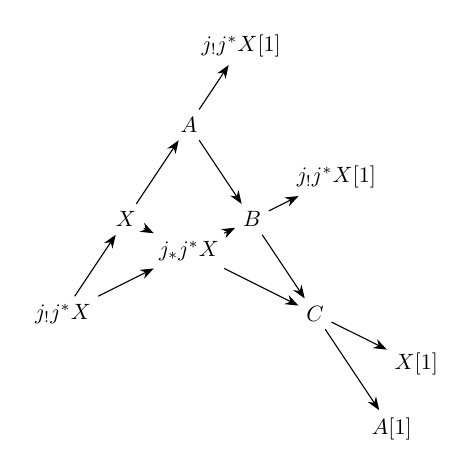
\begin{tikzpicture}[auto, >=Stealth, scale=0.8, transform shape]

  % Define coordinates for nodes
  \node (Z) at (0, 0) {$j_*j^*X$};
  \node (Y) at (-1, 0.5) {$X$};
  \node (X) at (-2, -1) {$j_!j^*X$};
  \node (Yp) at (1, 0.5) {$B$};
  \node (Zp) at (0, 2) {$A$};
  \node (Xp) at (2, -1) {$C$};
  \node (n1) at (0.83, 3.25) {$j_!j^*X[1]$};
  \node (n2) at (2.34, 1.17) {$j_!j^*X[1]$};
  \node (n3) at (3.61, -1.80) {$X[1]$};
  \node (n4) at (3.22, -2.83) {$A[1]$};

  % Draw arrows between nodes
  \draw[->] (X) to node[midway, above left] {} (Z);
  \draw[->] (Y) to node[midway, above right] {} (Z);
  \draw[->] (X) to node[midway, below] {} (Y);
  \draw[->] (Z) to node[midway, below] {} (Yp);
  \draw[->] (Z) to node[midway, below] {} (Xp);
  \draw[->] (Y) to node[midway, below] {} (Zp);
  \draw[->] (Zp) to node[midway, below] {} (Yp);
  \draw[->] (Yp) to node[midway, below] {} (Xp);
  \draw[->] (Zp) to node[midway, below] {} (n1);
  \draw[->] (Yp) to node[midway, below] {} (n2);
  \draw[->] (Xp) to node[midway, below] {} (n3);
  \draw[->] (Xp) to node[midway, below] {} (n4);
\end{tikzpicture}
\(\text{Based on } j_!j^*X \to X \to j_*j^*X\)
\end{minipage}
\end{center}
is unique up to unique isomorphism, and functorial in $X$.

(a) By (\rn{1.4.3.3}), (\rn{1.4.3.4}), and \rn{1.1.10}, there exists a unique isomorphism $A = i_* i^* X$, which identifies $X \to A$ with the adjunction morphism. It identifies $(j_! j^* X, X, A)$ with the distinguished triangle $(j_! j^* X, X, i_* i^* X)$ from (\rn{1.4.3.4}).

%% TRANSLATION-FIX: 1.4.7(b): B is the cone of j_!j^*X -> j_*j^*X, i.e. i_*i^*j_*j^*X; it is C that is i_*i^!X[1]
%% TRANSLATION-FIX: 1.4.7(b): an arrow into i_*i^*(-) is the unit of (i^*, i_*)
%% TRANSLATION-FIX: 1.4.7(b): with B corrected, A -> B is i_*i^* applied to X -> j_*j^*X
(b) The same argument, applied to $j_* j^* X$, which has the same $j^*$ as $X$, identifies $B$ with $i_* i^* j_* j^* X = i_* (j_*/j_!) j^* X$ (\rn{1.4.6.4})). The morphism $j_* j^* X \to B$ is the adjunction arrow of $(i^*, i_*)$. By \rn{1.1.9}, a unique morphism $A \to B$ makes the upper square of the octahedron commute. The morphism $A \to B$, i.e., $i_* i^* X \to i_* i^* j_* j^* X$, is thus the one deduced from $X \to j_* j^* X$ by functoriality.

%% TRANSLATION-FIX: 1.4.7(c): i^!X lies in D_F; the adjunction morphism is i_*i^!X -> X
%% TRANSLATION-FIX: 1.4.7(c): the second triangle of 1.4.3.4 is (i_*i^!X, X, j_*j^*X)
%% TRANSLATION-FIX: 1.4.7(c): by (1.4.6.4) j_*/j_! = i^!j_![1], and the map is i_*i^![1] of the counit j_!j^*X -> X
(c) Dually, there exists a unique isomorphism of $C$ with $i_* i^! X[1]$, identifying the degree $1$ arrow of $(X, j_* j^* X, C)$ with the adjunction morphism $i_* i^! X \to X$. The triangle $(X, j_* j^* X, C)$ is deduced from the triangle (\rn{1.4.3.4}) $(i_* i^! X, X, j_* j^* X)$ by rotation (TR 2), with a change of sign for the degree $1$ arrow $j_* j^* X \overset{(1)}\to i_* i^! X$. The morphism $B \to C$ is the unique one that makes the square $(B, C, j_* j^* X, X)$ commute. Via the isomorphism (\rn{1.4.6.4}) of $j_*/j_!$ with $i^!$, this morphism is $i_* (j_*/j_!) j^* X = i_* i^! j_! j^* X[1] \to i_* i^! X[1]$, deduced from $j_! j^* X \to X$ by functoriality.

(d) This determines all the vertices and arrows of the octahedron ($(C \overset{(1)}\to A$ is the composition $(C \overset{(1)}\to X\to A$) proves its functoriality. Replacing $A$, $B$, and $C$ with their values, it becomes:

\begin{center}
\begin{minipage}{0.45\textwidth}
\centering
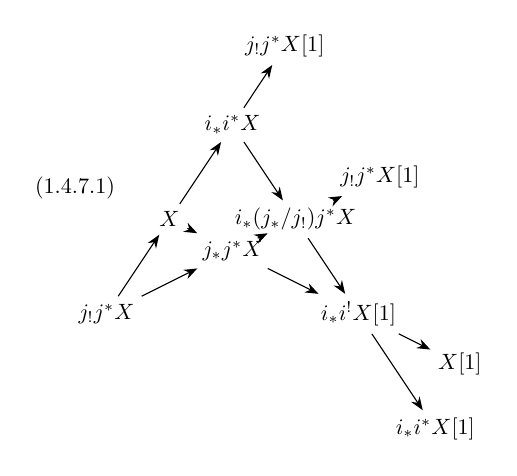
\begin{tikzpicture}[auto, >=Stealth, scale=0.8, transform shape]

  % Define coordinates for nodes
  \node (Z) at (0, 0) {$j_*j^*X$};
  \node (Y) at (-1, 0.5) {$X$};
  \node (X) at (-2, -1) {$j_!j^*X$};
  \node (Yp) at (1, 0.5) {$i_*(j_*/j_!)j^*X$};    \node (caption) at (-2.5,1) {(1.4.7.1)};
  \node (Zp) at (0, 2) {$i_*i^* X$};
  \node (Xp) at (2, -1) {$i_*i^!X[1]$};
  \node (n1) at (0.83, 3.25) {$j_!j^*X[1]$};
  \node (n2) at (2.34, 1.17) {$j_!j^*X[1]$};
  \node (n3) at (3.61, -1.80) {$X[1]$};
  \node (n4) at (3.22, -2.83) {$i_*i^* X[1]$};

  % Draw arrows between nodes
  \draw[->] (X) to node[midway, above left] {} (Z);
  \draw[->] (Y) to node[midway, above right] {} (Z);
  \draw[->] (X) to node[midway, below] {} (Y);
  \draw[->] (Yp) to node[midway, below] {} (Z);
  \draw[->] (Z) to node[midway, below] {} (Xp);
  \draw[->] (Y) to node[midway, below] {} (Zp);
  \draw[->] (Zp) to node[midway, below] {} (Yp);
  \draw[->] (Yp) to node[midway, below] {} (Xp);
  \draw[->] (Zp) to node[midway, below] {} (n1);
  \draw[->] (Yp) to node[midway, below] {} (n2);
  \draw[->] (Xp) to node[midway, below] {} (n3);
  \draw[->] (Xp) to node[midway, below] {} (n4);
\end{tikzpicture}
\end{minipage}
\end{center}

The functor $i_*$ being fully faithful, the distinguished triangle \( (i_* i^* X, i_* (j_*/j_!) j^* X, i_* i^! X[1]) \) is the $i_*$ of a triangle, automatically distinguished (\rn{1.3.19}), $(i^* X, (j_*/j_!) j^* X, i^! X[1])$. The $i_*$ of the degree $1$ arrow in this triangle is the composite $i_* i^! X[1]\overset{(1)} \to X \to i_* i^* X$, such that $d$ in {(\rn{1.4.6.1})} for $X[1]$ (the transform by $[1]$ of {(\rn{1.4.6.1})} for $X$). Rotating the triangle (TR 2), with a sign change for the new degree $1$ arrow and removing $i_*$ {(\rn{1.3.19})}, we obtain a functorial distinguished triangle
\[
(i^!, i^*, (j_*/j_!) j^*).\eqtag{1.4.7.2}
\]
Based on (\rn{1.4.6.1}). In the context of \rn{1.4.1} and \rn{1.4.2}, this triangle comes from the fact that for any flasque sheaf $F$, the sequence
\[
%% TRANSLATION-FIX: 1.4.7: i^!j_* = 0, so the third term is i^*j_*j^*F
0 \to i^! F \to i^* F \to i^* j_* j^* F \to 0
\]
is exact.

\bbdhead{Remark}{1.4.8} According to \cite{Verdier} §2, specifically pp. 23–27, the axioms (\rn{1.4.3.1}) to (\rn{1.4.3.5}) are equivalent to: "$i_*$ identifies $\mathcal{D}_F$ with a thick subcategory of $\mathcal{D}$, $j^*$ identifies $\mathcal{D}_U$ with $\mathcal{D}/\mathcal{D}_F$, and $j^*$ admits adjoints on the left and right."
\bbdhead{}{1.4.9}
Assume the hypotheses of (\rn{1.4.3}) are satisfied. Let $(\mathcal{D}_U^{\le 0}, \mathcal{D}_U^{\ge 0})$ define a $t$-structure on $\mathcal{D}_U$, and $(\mathcal{D}_F^{\le 0}, \mathcal{D}_F^{\ge 0})$ a $t$-structure on $\mathcal{D}_F$. Define:
\[
\mathcal{D}^{\le 0} := \{ K \in \mathcal{D} \mid j^* K \in \mathcal{D}_U^{\le 0} \ \text{and} \ i^* K \in \mathcal{D}_F^{\le 0} \},
\]
\[
\mathcal{D}^{\ge 0} := \{ K \in \mathcal{D} \mid j^* K \in \mathcal{D}_U^{\ge 0} \ \text{and} \ i^! K \in \mathcal{D}_F^{\ge 0} \}.
\]

\bbdhead{Theorem}{1.4.10}
\emph{With the hypotheses and previous notations, $(\mathcal{D}^{\le 0}, \mathcal{D}^{\ge 0})$ is a $t$-structure on $\mathcal{D}$. }

We say this $t$-structure is deduced from those of $\mathcal{D}_U$ and $\mathcal{D}_F$ by gluing.

We verify the axioms of \rn{1.3.1} \textbf{(i)}, \textbf{(ii)}, and \textbf{(iii)}.

\textbf{Axiom (i).} Let $X$ in $\mathcal{D}^{\le 0}$ and $Y$ in $\mathcal{D}^{\ge 1}$. The first distinguished triangle \textbf{(\rn{1.4.3.4})} for $X$ provides an exact sequence:
\[
\mathrm{Hom}(i_* i^* X, Y) \to \mathrm{Hom}(X, Y) \to \mathrm{Hom}(j_! j^* X, Y).
\]
We have $\mathrm{Hom}(i_* i^* X, Y) = \mathrm{Hom}(i^* X, i^! Y) = 0$, by \rn{1.3.1} (i) for $\mathcal{D}_F$, and $\mathrm{Hom}(j_! j^* X, Y) = \mathrm{Hom}(j^* X, j^* Y) = 0$, by \rn{1.3.1} (i) for $\mathcal{D}_U$. The assertion follows.

\textbf{Axiom (ii).} This trivially follows from \rn{1.3.1} (ii) for $\mathcal{D}_U$ and $\mathcal{D}_F$.

%% TRANSLATION-FIX: 1.4.10: must be j_*tau_{>0}j^*X, as the octahedron below and the computation use
\textbf{Axiom (iii).} Let $X$ be in $\mathcal{D}$. Choose $Y$, then $A$, resulting in distinguished triangles $(Y, X, j_* \tau_{> 0} j^* X)$ and $(A, Y, i_* \tau_{>0} i^* Y)$, and apply TR 4:

\begin{center}
\begin{minipage}{0.45\textwidth}
\centering
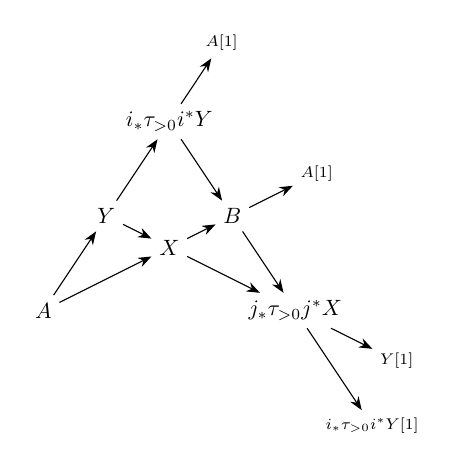
\begin{tikzpicture}[auto, >=Stealth, scale=0.8, transform shape]

  % Define coordinates for nodes
  \node (Z) at (0, 0) {$X$};
  \node (Y) at (-1, 0.5) {$Y$};
  \node (X) at (-2, -1) {$A$};
  \node (Yp) at (1, 0.5) {$B$};
  \node (Zp) at (0, 2) {$i_*\tau_{>0}i^*Y$};
  \node (Xp) at (2, -1) {$j_*\tau_{>0}j^*X$};
  \node (n1) at (0.83, 3.25) {$\scriptstyle A[1]$};
  \node (n2) at (2.34, 1.17) {$\scriptstyle A[1]$};
  \node (n3) at (3.61, -1.80) {$\scriptstyle Y[1]$};
  \node (n4) at (3.22, -2.83) {$\scriptstyle i_*\tau_{>0}i^*Y[1]$};

  % Draw arrows between nodes
  \draw[->] (X) to node[midway, above left] {} (Z);
  \draw[->] (Y) to node[midway, above right] {} (Z);
  \draw[->] (X) to node[midway, below] {} (Y);
  \draw[->] (Z) to node[midway, below] {} (Yp);
  \draw[->] (Z) to node[midway, below] {} (Xp);
  \draw[->] (Y) to node[midway, below] {} (Zp);
  \draw[->] (Zp) to node[midway, below] {} (Yp);
  \draw[->] (Yp) to node[midway, below] {} (Xp);
  \draw[->] (Zp) to node[midway, below] {} (n1);
  \draw[->] (Yp) to node[midway, below] {} (n2);
  \draw[->] (Xp) to node[midway, below] {} (n3);
  \draw[->] (Xp) to node[midway, below] {} (n4);
\end{tikzpicture}
\end{minipage}
\end{center}

Apply the functors $j^*, i^*$, and $i^!$ to the distinguished triangles of this octahedron, according to the following scheme, taking into account {(\rn{1.4.3.3})} to {(\rn{1.4.3.5})}:
\begin{align*}
&j^* (i_* \tau_{>0} i^* Y, B, j_* \tau_{> 0} j^* X) = (0, j^* B, \tau_{> 0} j^* X),&\mbox{ hence }j^*B\overset{\sim}{\to}\tau_{>0}j^*X\\
&j^* (A, X, B) = (j^* A, j^* X, \tau_{>0} j^* X),&\mbox{ hence }j^*A\overset{\sim}{\to}\tau_{\le0}j^*X\\
&i^* (A, Y, i_* \tau_{>0} i^* Y) = (i^* A, i^* Y, \tau_{>0} i^* Y), &\mbox{ hence }i^*A\overset{\sim}{\to}\tau_{\le 0}i^*Y,\\
&i^! (i_*\tau_{>0}i^*Y,B,j_*\tau_{>0}j^*X) = (\tau_{>0}i^*Y,i^!B,0), &\mbox{ hence }\tau_{> 0}i^*Y\overset{\sim}{\to}i^!B.
\end{align*}
Thus, $A$ is in $\mathcal{D}^{\leq 0}$ and $B$ is in $\mathcal{D}^{\geq 1}$, and $(A, X, B)$ satisfies \textbf{(\rn{1.3.1})} (iii).

\bbdhead{Remark}{1.4.11} For the $t$-structure obtained on $\mathcal{D}$ to be non-degenerate, it is necessary and sufficient that the $t$-structures given on $\mathcal{D}_U$ and $\mathcal{D}_F$ are non-degenerate.
We will not use, in the remainder of these notes, the reciprocal result corresponding to {\rn{1.4.10}}.

\bbdhead{Proposition}{1.4.12}
\emph{Under the hypotheses and with the notations of \textbf{\rn{1.4.3}}, let $(\mathcal{D}^{\leq 0}, \mathcal{D}^{\geq 0})$ be a $t$-structure on $\mathcal{D}$. The following conditions are equivalent:}

\emph{(i) $j_! j^*$ is $t$-exact on the right;}

\emph{(i') $j_* j^*$ is $t$-exact on the left;}

\emph{(ii) The $t$-structure on $\mathcal{D}$ is obtained by gluing.}

The equivalence $(i) \iff (\text{i}')$ results from {\rn{1.3.17}} (iii), and $(i)$ and $(\text{i}')$ are equivalent to the axiom {\rn{1.3.1} (i)} for $(j^*\mathcal{D}^{\leq 0}, j^*\mathcal{D}^{\geq 0})$. The distinguished triangles $(j_!j^*, \mathrm{Id}, i_* i^*)$ and $(i_* i^!, \mathrm{Id}, j_* j^*)$ respectively show that $(i)$ and $(\text{i}')$ imply that $i_* i^*$ is $t$-exact on the right and $i_* i^!$ is $t$-exact on the left—conditions that are also equivalent to {\rn{1.3.17}} (iii), and imply that $(i^* \mathcal{D}^{\leq 0}, i^! \mathcal{D}^{\geq 0})$ satisfies the axiom {\rn{1.3.1} (i)}.

It is clear that $(ii) \implies (i), (\text{i}')$, and that the $t$-structures on $\mathcal{D}_U$ and $\mathcal{D}_F$ obtained by gluing are, respectively, $(j^* \mathcal{D}^{\leq 0}, j^* \mathcal{D}^{\geq 0})$ on $\mathcal{D}_U$ that is induced by that of $\mathcal{D}$ and on $\mathcal{D}_F$: $( \mathcal{D}_F\cap \mathcal{D}^{\leq 0}, \mathcal{D}_F\cap \mathcal{D}^{\geq 0})\cong(i^* \mathcal{D}^{\leq 0},i^! \mathcal{D}^{\geq 0})$ . Conversely, if $(i)$ and $(\text{i}')$ are satisfied, we successively verify the following:

%% TRANSLATION-FIX: 1.4.12(a): the image t-structure on D_U is (j^*D^{<=0}, j^*D^{>=0})
(a) $(j^* \mathcal{D}^{\leq 0}, j^* \mathcal{D}^{\geq 0})$ is a $t$-structure on $\mathcal{D}_U$. {\rn{1.3.1} (i)} has already been verified, {\rn{1.3.1} (ii)} is clear, and {\rn{1.3.1} (iii)} follows from $j^*$ being essentially surjective.

%% TRANSLATION-FIX: 1.4.12(b): the t-structure on D_F is (i^*D^{<=0}, i^!D^{>=0})
(b) $(i^* \mathcal{D}^{\leq 0}, i^! \mathcal{D}^{\geq 0})$ is a $t$-structure on $\mathcal{D}_F$. {\rn{1.3.1} (i)} has already been verified. Only {\rn{1.3.1} (iii)} is non-trivial: for $X$ in $\mathcal{D}_F$, the $t$-exactness of $j^*$ shows that $j^* \tau_{\leq 0}i_* X = \tau_{\leq 0} j^* i_*X = 0$ and similarly $j^* \tau_{> 0}i_* X= 0$. The truncations $\tau_{\leq 0}i_* X$ and $\tau_{> 0} i_* X$ are thus in $i_* \mathcal{D}_F$: they form a triangle $(i^* \tau_{\leq 0} i_* X, X,i^* \tau_{> 0}i_* X)$ that satisfies {\rn{1.3.1} (iii)}.

%% TRANSLATION-FIX: 1.4.12(c): the two t-structures glued are the ones just constructed in (a) and (b)
(c) The identity functor on $\mathcal{D}$, equipped with its $t$-structure, ...of the glued $t$-structure $(j^* \mathcal{D}^{\leq 0}, j^* \mathcal{D}^{\geq 0})$ and $(i^* \mathcal{D}^{\leq 0}, i^! \mathcal{D}^{\geq 0})$ is $t$-exact. According to \rn{1.3.19}, the $t$-structure is therefore obtained by gluing.

\bbdhead{}{1.4.13}
%% TRANSLATION-FIX: 1.4.12: circular as printed; it is tau_{<=p} of the glued t-structure that is renamed
Assume only that a $t$-structure exists on $\mathcal{D}_F$, and apply \rn{1.4.10} to the degenerate $t$-structure $(\mathcal{D}_U, 0)$ on $\mathcal{D}_U$ and the $t$-structure on $\mathcal{D}_F$. The functors $\tau_{\leq p}$ related to the $t$-structure obtained on $\mathcal{D}$ are denoted $\tau_{\leq p}^F$. The functor $\tau_{\leq p}^F$ is right adjoint to the inclusion of the thick subcategory of $\mathcal{D}$ consisting of $X$ such that $i^* X$ is in $\mathcal{D}_F^{\leq p}$. The proof of \rn{1.4.10} for axiom \rn{1.3.1} (iii) provides a distinguished triangle
\[
(\tau_{\leq p}^F X, X, i_* \tau_{\geq p+1} i^* X)
\]
(with the notations of \rn{1.4.10}, we have $X=Y$). The successive $\mathrm{H}^p$ for this $t$-structure are thus $i_* \mathrm{H}^p i^* X$.

Dually, we define $\tau_{\geq p}^F$ in terms of the degenerate $t$-structure $(0, \mathcal{D}_U)$ on $\mathcal{D}_U$; it is the left adjoint to the inclusion of $(i^!)^{-1} \mathcal{D}_F^{\geq p}$ into $\mathcal{D}$. We have a distinguished triangle
\[
(i_* \tau_{\leq p-1} i^! X, X, \tau_{\geq p}^F X),
\]
and the successive $\mathrm{H}^p$ are $i_* \mathrm{H}^p i^! X$.

Similarly, if we assume only that a $t$-structure exists on $\mathcal{D}_U$ and equip $\mathcal{D}_F$ with the $t$-structure $(\mathcal{D}_F^{\leq 0}, \mathcal{D}_F^{\geq 0})$, we define on $\mathcal{D}$ a $t$-structure for which the functors $\tau_{\leq p}^U$ (resp. $\tau_{\geq p}^U$) result in distinguished triangles:
\[
(\tau_{\leq p}^U X, X, j_* \tau_{\geq p+1} j^* X) \quad \text{(resp. } (j_! \tau_{\leq p-1} j^* X, X, \tau_{\geq p}^U X) \text{)},
\]
and for which the successive $\mathrm{H}^p$ are $j_* \mathrm{H}^p j^* X$ (resp. $j_! \mathrm{H}^p j^* X$).

The proof of \rn{1.4.10} for axiom (iii) shows that $\tau_{\leq 0} = \tau_{\leq 0}^F \tau_{\leq 0}^U$ and $\tau_{\geq 0} = \tau_{\geq 0}^F \tau_{\geq 0}^U$.

Translating and dualizing, we obtain
\[
\tau_{\leq p} = \tau_{\leq p}^F \tau_{\leq p}^U \quad \text{and} \quad \tau_{\geq p} = \tau_{\geq p}^F \tau_{\geq p}^U.
\eqtag{1.4.13.1}\]

In the situation of \rn{1.4.1} and for the natural $t$-structure on $\mathcal{D}^+ (F, \mathcal{O})$, the functor $\tau_{\leq p}^F$ is deduced from the functor in the category of sheaf complexes itself, which associates to a complex $K$ its subcomplex coinciding with $K$ over $U$ and with the subcomplex $\tau_{\leq p}$ (\textbf{\rn{1.3.2}}) on $F$.

%% TRANSLATION-FIX: 1.4.13: tau^U does not preserve j^*, and j_! pairs with >=, j_* with <=
%% TRANSLATION-FIX: 1.4.13: same correction in the following clause
Call a \emph{extension} of an object $Y$ in $\mathcal{D}_U$ an object $X$ in $\mathcal{D}$, equipped with an isomorphism $j^* X \cong Y$. Such an isomorphism gives rise, by adjunction, to morphisms $j_! Y \to X \to j_* Y$. If an extension $X$ is isomorphic, as an extension, to $\tau_{\geq p}^F j_! Y$ (resp. $\tau_{\leq p}^F j_* Y$), the isomorphism is unique, and we simply say that $X = \tau_{\geq p}^F j_! Y$ (resp. $X = \tau_{\leq p}^F j_* Y$).

\bbdhead{Proposition}{1.4.14}
%% TRANSLATION-FIX: 1.4.14: tau^F_{<=p}j_!Y = j_!Y since i^*j_! = 0; the extension is tau^F_{>=p+1}j_!Y = tau^F_{<=p-1}j_*Y
\emph{Let $Y$ be in $\mathcal{D}_U$ and $p$ an integer. There exists, up to unique isomorphism, one and only one extension $X$ of $Y$ such that $i^* X$ is in $\mathcal{D}_F^{\leq p-1}$ and $i^! X$ is in $\mathcal{D}_F^{\geq p+1}$. It is $\tau_{\geq p+1}^F j_! Y = \tau_{\leq p-1}^F j_* Y$.}

Let $X$ be an extension of $Y$. The distinguished triangle \( (i^* X, (j_*/j_!) Y, i^! X[1]) \) from \rn{1.4.7.2} deduced by rotation shows that the following conditions are equivalent:

(a) $i^* X$ is in $\mathcal{D}_F^{\leq p-1}$ and $i^! X$ is in $\mathcal{D}_F^{\geq p+1}$.

(b) $i^! X[1]$ is $\tau_{\geq p}$ of $ (j_*/j_!) Y = i^* j_* Y$.

%% TRANSLATION-FIX: 1.4.14: this triangle controls i^!X[1], i.e. condition (b); (b') is treated dually next
(b') $i^* X$ $\tau_{\leq p-1}$ of $(j_*/j_!) Y$. The distinguished triangle $(X, j_* Y, i_* i^! X[1])$ from 1.4.7.1 shows that (b) is equivalent to $X = \tau_{\leq p-1}^F j_* Y$. Dually, (b') is equivalent to $X = \tau_{\geq p+1}^F j_! Y$.

\bbdhead{Remark}{1.4.14.1} Let $\mathcal{D}_m$ be the thick subcategory of $\mathcal{D}$ formed by objects $X$ verifying the conditions $i^* X \in \mathcal{D}_F^{\leq p-1}$ and $i^! X \in \mathcal{D}_F^{\geq p+1}$ of \rn{1.4.14}. The functor $j^*$ induces an equivalence of categories $\mathcal{D}_m \to \mathcal{D}_U$. It admits as quasi-inverse the extension functor $\tau_{\leq p-1}^F j_*$. We will sometimes denote ${}^pj_{!*}$ as the quasi-inverse.
\bbdhead{}{1.4.15}
%% TRANSLATION-FIX: 1.4.15: T is reused below as the generic functor; the inclusions of the hearts are the epsilon
Let $\mathcal{C}, \mathcal{C}_U, \mathcal{C}_F$ be the hearts of the $t$-structures on $\mathcal{D}, \mathcal{D}_U, \mathcal{D}_F$, and $\mathcal{D}$ be equipped with the glued $t$-structure of \rn{1.4.10}. Let the inclusions of $\mathcal{C}, \mathcal{C}_U, \mathcal{C}_F$ into $\mathcal{D}, \mathcal{D}_U, \mathcal{D}_F$, respectively, be noted $\epsilon$. For one of the functors $j_!, j^*, j_*, i_*, i^*, i^!$, let ${}^p T$ denote the functor $H^0\circ T\circ \epsilon$.

By definition of the $t$-structure on $\mathcal{D}$, $j^*$ is $t$-exact, $i^*$ is $t$-exact on the right, and $i^!$ is $t$-exact on the left. Applying \rn{1.3.17} (iii), we obtain:

\bbdhead{Proposition}{1.4.16}
\emph{(i) The functors $j_!$ and $i^*$ (resp. $j^*$ and $i_*$, resp. $j_*$ and $i^!$) are $t$-exact on the right (resp. $t$-exact, resp. $t$-exact on the left).}

\emph{(ii) $({}^p j_!, {}^p j^*, {}^p j_*)$ and $({}^p i^*, {}^p i_*, {}^p i^!)$ form two sequences of three adjoint functors.}

\bbdhead{Proposition}{1.4.17}
%% TRANSLATION-FIX: 1.4.17(i): as printed the first two composites are not composable; cf. 1.4.3.3
\emph{(i) The composites ${}^p j^* \circ {}^p i_*, {}^p i^* \circ {}^p j_!, {}^p i^! \circ {}^p j_*$ vanish. For $A$ in $\mathcal{C}_F$ and $B$ in $\mathcal{C}_U$, we have
\[
\mathrm{Hom}({}^p j_! B, {}^p i_* A) = \mathrm{Hom}({}^p i_* A, {}^p j_* B) = 0.
\]}

\emph{(ii) For any $A$ in $\mathcal{C}$, the sequences
\[
{}^p j_! {}^p j^* A \to A \to {}^p i_* {}^p i^* A \to 0
\]
and
\[
0 \to {}^p i_*{}^p  i^! A \to A \to {}^p j_* {}^p j^* A
\]
are exact. }

%% TRANSLATION-FIX: 1.4.17(iii): ^pj^* is a quotient functor; the fully faithful ones are ^pi_*, ^pj_!, ^pj_*
\emph{(iii) ${}^p i_*$, ${}^p j_!$, and ${}^p j_*$ are fully faithful: the adjunction morphisms
\[
%% TRANSLATION-FIX: 1.4.17(iii): the counit is j^*j_! -> Id and the unit Id -> j^*j_*
{}^p i^* {}^p i_* \to \mathrm{Id}\to {}^p i^! {}^p i_*, \quad \text{and} \quad {}^p j^* {}^p j_! \to \mathrm{Id} \to {}^p j^* {}^p j_*
\]
are isomorphisms.}

These assertions respectively follow from {(\rn{1.4.3.3})}, 4, and 5. The verification is left to the reader (see \rn{1.3.17} (iv)).

\bbdhead{Amplification}{1.4.17.1}
From (i) $({}^p j^* {}^p i_* = 0)$ and any of the exact sequences (ii), for $X$ in $\mathcal{C}$ to lie in the essential image $\overline{\mathcal{C}}_F$ of ${}^p i_*$, it is necessary and sufficient that ${}^p j^* X = 0$. The functor ${}^p j^*$ being exact, this essential image is a thick subcategory (i.e., stable under extensions and subquotients) of $\mathcal{C}$. If we identify $\mathcal{C}_F$ as the thick subcategory of $\mathcal{C}$ via the fully faithful functor ${}^p i_*$, the adjunctions \( ({}^p i^*, {}^p i_*), \quad \text{and} \quad ({}^p i_*, {}^p i^!) \) ({(\rn{1.4.16})} (ii)) show that for $X$ in $\mathcal{C}$, ${}^p i^* X$ is the largest quotient of $X$ in $\overline{\mathcal{C}}_F$, and ${}^p i^! X$ is the largest subobject of $X$ in $\mathcal{C}_F$.

\bbdhead{Proposition}{1.4.18}
\emph{The functor ${}^p j^*$ identifies $\mathcal{C}_U$ with the quotient of $\mathcal{C}$ by the thick subcategory $\mathcal{C}_F$ (or, more precisely, $\overline{\mathcal{C}}_F$, see \rn{1.4.17.1}).}

Let $Q: \mathcal{C} \to \mathcal{C}/\mathcal{C}_F$ be the functor for passing to the quotient. The exact functor ${}^p j^*$ admits a factorization $T \circ Q$, and $T$ is faithful: If $f$ in $\mathcal{C}/\mathcal{C}_F$ comes from $f_1$ in $\mathcal{C}$, if $f$ is killed by $T$ then $f_1$ is killed by ${}^pj^*$, i.e. $\mathrm{Im}(f_1)$ lies in the image of $\mathcal{C}_F$, and $f_1$ is killed by $Q$. Since $\mathrm{Id} \overset{\sim}\to {}^p j^*{}^p j_!= T \circ Q \circ {}^p j_!$ is surjective on isomorphism classes of objects, it remains to verify that $T$ is fully faithful, which then gives an equivalence of categories.

\bbdhead{Lemma}{1.4.19}
\emph{For any $A$ in $\mathcal{C}$, the sequences
\[
%% TRANSLATION-FIX: 1.4.19: this sequence comes from (j_!j^*A, A, i_*i^*A), so the first term uses i^*
0 \to {}^p i_* H^{-1} i^* A \to {}^p j_! {}^p j^* A \to A \to {}^p i_* {}^p i^* A \to 0
\]
and
\[
0 \to {}^p i_* {}^p i^! A \to A \to {}^p j_* {}^p j^* A \to {}^pi_*H^1i^!A\to 0
\]
are exact.}

The result follows from {(\rn{1.4.3.4})} and {(\rn{1.4.16})} (i).

We now complete the proof of \textbf{\rn{1.4.18}}. By \rn{1.4.19}, the kernel and cokernel of ${}^p j_! {}^p j^* A \to A$ are in the image of ${}^p i_*$. Every object of $\mathcal{C}/{}^p i_*\mathcal{C}_F$ therefore has a representative in the image of ${}^p j_!$. For ${}^p j_! X$ and ${}^p j_! Y$ in this image,
\[
T: \mathrm{Hom}(Q{}^p j_! X, Q{}^p j_! Y) \to \mathrm{Hom}(TQ {}^p j_! X, TQ {}^p j_! Y) = \mathrm{Hom}(X, Y)
\]
admits a section $Q {}^p j_!$, and thus is surjective. This completes the proof.

\subsection*{\texorpdfstring{\anch{1.4.20}}{1.4.20} Warning}
Under the hypotheses of \rn{1.4.1}, when $\mathcal{D}^+(U, \mathcal{O})$ and $\mathcal{D}^+(F, \mathcal{O})$ are equipped with their natural $t$-structure (\rn{1.3.2} (i)), the $t$-structure obtained on $\mathcal{D}^+(X, \mathcal{O})$ is the natural $t$-structure, and the abelian categories $\mathcal{C}, \mathcal{C}_U$, and $\mathcal{C}_F$ are $\mathcal{M}(X, \mathcal{O}), \mathcal{M}(U, \mathcal{O})$, and $\mathcal{M}(F, \mathcal{O})$, respectively. We recover the situation of \rn{1.4.1}.

%% TRANSLATION-FIX: 1.4.20: j_! and i^* are right t-exact, so ^pj_! and ^pi^* are right exact
In general, however, ${}^p j_!$ is right exact but not exact, ${}^p i^*$ is right exact but not exact, and the first sequence in \rn{1.4.17} (ii) is not left exact. The formalism of \rn{1.4.3}, being self-dual, ensures that only the formulas valid in the context of \rn{1.4.1}, along with their duals, remain universally true.

\bbdhead{}{1.4.21}
Let us revisit the arguments of \rn{1.4.6}.

(a) The functor ${}^p i_*$, being fully faithful, the composite of the adjunction morphisms
\[
{}^p i_* {}^p i^! \to \mathrm{Id} \to {}^p i_* {}^p i^*
\]
%% TRANSLATION-FIX: 1.4.21(a): the composite is deduced from a unique morphism ^pi^! -> ^pi^*
is deduced from a unique morphism of functors:
\[
 {}^p i^! \to  {}^p i^*.
\eqtag{1.4.21.1}\]
%% TRANSLATION-FIX: 1.4.21: i^* is only right t-exact; what is used is the t-exactness of i_*
The commutative diagrams \rn{1.3.18} (ii) for $(i^*, i_*)$ and $(i_*, i^!)$, and the $t$-exactness of $i_*$, provide for $A$ in $\mathcal{C}$ a commutative diagram:
\[
\begin{tikzcd}
{}^p i_* {}^p i^! A \ar[r] \ar[d,equals] & A \ar[r] \ar[dd,equals] & {}^p i_* {}^p i^* A \ar[d,equals] \\
i_* {}^p i^! A \ar[d] && i_* {}^p i^* A \\
i_* i^! A \ar[r] & A \ar[r] & i_* i^* A \ar[u]
\end{tikzcd}
\]
From this, it follows that for $A$ in $\mathcal{C}$, the morphism (\rn{1.4.21.1}): \( {}^p i^! A \to {}^p i^* A \) is the composition
\[
 {}^p i^! A \to i^!A\xrightarrow{\text{(1.4.6.1)}} i^*A\to  {}^p i^* A. \eqtag{1.4.21.2}
\]
When we apply (\rn{1.4.21.1}) to $i_* A$ (with $A$ in $\mathcal{C}_F$), we obtain the identity automorphism of $A$.

(b) The functor ${}^p j^*$, being a quotient passage functor (\rn{1.4.18}), the composite of the adjunction morphisms \( {}^p j_! {}^p j^* \to \mathrm{Id} \to {}^p j_* {}^p j^* \) arises from a unique morphism of functors:
\[
{}^p j_! \to {}^p j_*. \eqtag{1.4.21.3}
\]
The commutative diagrams \rn{1.3.18} (ii) for $(j^*, j_*)$ and $(j_!, j^*)$, along with the $t$-exactness of $j^*$, provide for $A$ in $\mathcal{C}$ a commutative diagram:
\[
\begin{tikzcd}
{}^p j_! {}^p j^* A \ar[r] \ar[d,equals] & A \ar[r] \ar[dd,equals] & {}^p j_* {}^p j^* A \ar[d,equals] \\
{}^p j_! j^* A  &&  {}^p j_*  j^* A \ar[d] \\
j_! j^* A \ar[u] \ar[r] & A \ar[r] &  j_* j^* A
\end{tikzcd}
\]
%% TRANSLATION-FIX: 1.4.21: (1.4.6.2) is the morphism j_! -> j_*
From this, it follows that for $B$ in $\mathcal{C}_U$, the morphism (\rn{1.4.6.2}) of $j_! B$ in $j_* B$ is the composite:
\[
j_! B \to \tau_{\geq 0} j_! B = {}^p j_! B\xrightarrow{\text{(1.4.21.3)}}{}^p j_*B=\tau_{\le 0}j_* B\to j_*B. \eqtag{1.4.21.4}
\]
%% TRANSLATION-FIX: 1.4.21: (1.4.21.3) is ^pj_! -> ^pj_*; an identity has no kernel or cokernel
When applying ${}^p j^*$ to (\rn{1.4.21.3}), we find the identity automorphism of the identity functor. In particular, for $B$ in $\mathcal{C}_U$, the kernel and cokernel of (\rn{1.4.21.3}), ${}^p j_! B \to {}^p j_* B$, are in ${}^p i_* \mathcal{C}_F$.

\bbdhead{Definition}{1.4.22}
The functor $j_{!*}:\cC_{U}\to\cC$ is the functor which to $B$ in $\cC_{U}$ attaches the image of $\p{j_{!}}B$ in $\p{j_{*}}B$.

For $B$ in $\mathcal{C}_U$, (\rn{1.4.21.4}) provides the following factorization of the morphism (\rn{1.4.6.2}) of $j_! B$ in $j_* B$:
\[
j_! B \to {}^p j_! B \to j_{!*} B \to {}^p j_* B \to j_* B. \eqtag{1.4.22.1}
\]

\bbdhead{Proposition}{1.4.23}
\emph{For $B$ in $\mathcal{C}_U$, we have:
\begin{align*}
{}^p j_! B & = \tau_{\geq 0}^F j_! B = \tau_{\leq -2}^F j_* B,\\
j_{!*} B &= \tau_{\geq 1}^F j_! B = \tau_{\leq -1}^F j_* B,\\
{}^p j_* B &= \tau_{\geq 2}^F j_! B = \tau_{\leq 0}^F j_* B.
\end{align*}
%% TRANSLATION-FIX: 1.4.23: tau^F_{>=0}j_!B is ^pj_!B; ^pj_*B is tau^F_{>=2}j_!B
More precisely, ${}^p j_! B$, equipped with the map $j_! B \to {}^p j_! B$, is $\tau_{\geq 0}^F j_! B$, and so on.}

Since $j^* j_! B$ is in $\mathcal{C}_U$, $j_! B$ is its own proper ${\tau}^U_{\geq 0}$. By \rn{1.4.13.1}, we thus have ${}^p j_! B = \tau_{\geq 0} j_! B = \tau_{\geq 0}^F j_! B$; by \rn{1.4.14}, \( \tau_{\geq 0}^F j_! B = \tau_{\leq -2}^F j_* B. \) Likewise $\p{j_{*}}B=\tau_{\leq 0}j_{*}B=\tau^{F}_{\leq 0}j_{*}B$.

The determination in \rn{1.4.13} of $\mathrm{H}^p$ for the $t$-structure defining ${}^F_{\geq p}$ provides a distinguished triangle:
\[
(i_* \mathrm{H}^{0} i^! j_! B, {\tau}^F_{\geq 0}j_! B, {\tau}^F_{\geq 1}j_! B).
\]
%% TRANSLATION-FIX: 1.4.23: the first two terms of the triangle lie in the heart, so the third is in D^{[0,1]}
This shows that $\tau_{\geq 1}^F j_! B$ is in $\mathcal{D}^{[0, 1]}$. A dual argument provides a distinguished triangle: \(
%% TRANSLATION-FIX: 1.4.23: B lies in C_U, so i^*B is undefined; the functor is applied to j_*B
({\tau}^F_{\leq -1}j_* B, {\tau}^F_{\leq 0} j_* B, i_*H^0i^*j_* B), \)
%% TRANSLATION-FIX: 1.4.23: the last two terms lie in the heart, so the first is in D^{[-1,0]}
showing that ${\tau}^F_{\leq -1} j_* B$ is in $\mathcal{D}^{[-1, 0]}$. Applying \rn{1.4.14}, we find that ${\tau}^F_{\leq- 1} j_* B$ is ${\tau}^F_{\geq 1} j_! B$, and the above triangles become short exact sequences:
\[
0 \to i_* \mathrm{H}^{0} i^! j_! B \to {}^p j_! B \to {\tau}^F_{\geq 1} j_! B \to 0
\]
\[
0 \to \tau^F_{\leq -1} j_* B \to {}^p j_* B \to i_* \mathrm{H}^{0} i^* j_* B \to 0
\]
%% TRANSLATION-FIX: 1.4.23: 1.4.22 defines j_{!*}B as the image of ^pj_!B, not of j_!B
These show that $\tau_{\geq 1}^F j_! B = {\tau}^F_{\leq -1} j_* B$ is indeed the image $j_{!*}B$ of ${}^p j_! B$ in ${}^p j_* B$.

\bbdhead{Corollary}{1.4.24}
\emph{For $B$ in $\mathcal{C}_U$, $j_{!*} B$ is the unique extension $X$ of $B$ in $\mathcal{D}$ such that $i^* X$ is in $\mathcal{D}_F^{\leq -1}$ and $i^! X$ is in $\mathcal{D}_F^{\geq 1}$.}

Applying \rn{1.4.14}, similarly, ${}^p j_! B$ (resp. ${}^p j_* B$) is the unique extension $X$ such that $i^* X$ is in $\mathcal{D}_F^{\leq -2}$ (resp. $\mathcal{D}_F^{\leq 0}$) and $i^! X$ is in $\mathcal{D}_F^{\geq 0}$ (resp. $\mathcal{D}_F^{\geq 2}$).

\bbdhead{Corollary}{1.4.25}
\emph{For $B$ in $\mathcal{C}_U$, $j_{!*} B$ is the unique extension $X$ of $B$ in $\mathcal{C}$ without any non-trivial subobject or quotient lying in the essential image $\overline{\mathcal{C}}_F$ of $\mathcal{C}_F$ under $i_*$.}

By definition $j_{!*}B$ lies in $\cC\subset\D$; for $X$ in $\cC$ an extension of $B$, one has $i^{*}X\in\D_{F}^{\leq 0}$, and $i^{*}X\in\D_{F}^{\leq -1}$ if and only if $\p{i^{*}}X=0$. Dually, $i^{!}X$ lies in $\D_{F}^{\geq 1}$ if and only if $\p{i^{!}}X=0$. Identify $\cC_{F}$ with $\overline{\cC}_{F}$ by $i_{*}$. Since $\p{i^{*}}X$ (resp.\ $\p{i^{!}}X$) is the largest quotient (resp.\ subobject) of $X$ lying in $\cC_{F}$ (\rn{1.4.17.1}), the characterization \rn{1.4.25} of $j_{!*}B$ is a reformulation of \rn{1.4.24}.

\bbdhead{Proposition}{1.4.26}
\emph{The simple objects of $\mathcal{C}$ are the ${}^p i_* S$, for $S$ simple in $\mathcal{C}_F$, and the $j_{!*} S$, for $S$ simple in $\mathcal{C}_U$.}

Since the essential image $\overline{\mathcal{C}}_F$ of $\mathcal{C}_F$ under ${}^p i_*$ is a thick subcategory of $\mathcal{C}$, for $S$ in $\mathcal{C}$ to be simple, it is necessary and sufficient that either: (a) $S$ is in $\overline{\mathcal{C}}_F$, and simple in $\overline{\mathcal{C}}_F$, or (b) $S$ has an image simple in $\mathcal{C}/\overline{\mathcal{C}}_F$, and no non-trivial subobject or quotient in $\overline{\mathcal{C}}_F$. Case (a) gives the ${}^p i_* S$ of simple objects of $\mathcal{C}_F$, while using \rn{1.4.25}, case (b) gives the $j_{!*}$ of simple objects of $\mathcal{C}_U$.

\chapter{Perverse Sheaves on Stratified Spaces and on Schemes}

\section{Stratified Spaces}

\num{\anch{2.1.1}.}
Let $X$ be a topological space equipped with a sheaf of rings $\mathcal{O}$, let $S$ be a finite partition of $X$ into locally closed subsets (called \emph{strata}) and $p$ a function $S\to\mathbb{Z}$ (called the \emph{perversity}). By definition of ``partition'', the strata are non-empty. We assume that the closure of each stratum is a union of strata. These conditions may be relaxed: see \rn{3.2.19}.

Recall (0.0) that for $f:X\to Y$ we shall write simply $f_{!},f_{*},f^{!},f^{*}$ for the functors between derived categories usually written $Rf_{!},Rf_{*},Rf^{!},Rf^{*}$ (or $Lf^{*}$). For a reason explained in \rn{2.1.7}, the analogous functors between categories of sheaves will be written with a superscript $o$ on the left.

\num{Definition \anch{2.1.2}.}
\emph{The subcategory $\p{D^{\leq0}}(X,\mathcal{O})$ (resp.\ $\p{D^{\geq0}}(X,\mathcal{O})$) of $D(X,\mathcal{O})$ is the subcategory formed by the complexes $K$ (resp.\ $K$ in $D^{+}(X,\mathcal{O})$) such that for each stratum $S$, writing $i_{S}$ for the inclusion of $S$ into $X$, one has $H^{n}i_{S}^{*}K=0$ for $n>p(S)$ (resp.\ $H^{n}i_{S}^{!}K=0$ for $n<p(S)$).}

\smallskip
The exactness of the functors $\,^{o}i^{*}$ allows one to reformulate the definition of $\p{D^{\leq0}}(X,\mathcal{O})$: in order for $K$ to lie in $\p{D^{\leq0}}(X,\mathcal{O})$ it is necessary and sufficient that the restriction of $H^{i}K$ to $S$ vanish for $i>p(S)$. The functors $\tau_{\leq a}$ and $\tau_{\geq a}$, relative to the natural t-structure, therefore map $\p{D^{\leq0}}(X,\mathcal{O})$ into itself.

If the functors $\,^{o}i_{S}^{!}$ are of finite cohomological dimension, the functor $i_{S}^{!}:D^{+}(X,\mathcal{O})\to D^{+}(S,\mathcal{O})$ has a natural extension $D(X,\mathcal{O})\to D(S,\mathcal{O})$, and the condition ``$H^{n}i_{S}^{!}K=0$ for $n<p(S)$'' makes sense for $K$ not necessarily in $D^{+}(X,\mathcal{O})$. It nevertheless implies that $K$ lies in $D^{+}(X,\mathcal{O})$. More precisely, if $p\geq a$ it implies that $K$ lies in $D^{\geq a}(X,\mathcal{O})$: let us check by descending induction on the stratum $S$ --- for the order $S_{1}\subset\overline{S}_{2}$ --- that the $H^{i}K$ vanish on $S$ for $i<a$. For $i<a$, the triangle $(\tau_{<a}K,\,K,\,\tau_{\geq a}K)$ and the left exactness of $\,^{o}i_{S}^{!}$ show that $H^{i}i_{S}^{!}\tau_{<a}K\iso H^{i}i_{S}^{!}K$. The induction hypothesis ensures that the $H^{j}\tau_{<a}K$ vanish on the strata $T\neq S$ such that $S\subset\overline{T}$, hence that $S$ has a neighbourhood in which $H^{j}\tau_{<a}K$ has support in $S$. For $i<a$ one thus has
\[
H^{i}K|S=H^{i}i_{S}^{*}\tau_{<a}K=H^{i}i_{S}^{!}\tau_{<a}K=H^{i}i_{S}^{!}K,
\]
and this last group vanishes by hypothesis.

\num{\anch{2.1.2.1}.}
Without any hypothesis of cohomological dimension, the same argument applies for $K$ in $K^{+}(X,\mathcal{O})$. If the integers $a$ and $b$ are such that $a\leq p\leq b$, one has
\[
(2.1.2.1)\qquad D^{\leq a}(X,\mathcal{O})\subset \p{D^{\leq 0}}(X,\mathcal{O})\subset
D^{\leq b}(X,\mathcal{O})
\]
and
\[
D^{\geq a}(X,\mathcal{O})\supset \p{D^{\geq 0}}(X,\mathcal{O})\supset
D^{\geq b}(X,\mathcal{O}).
\]
We write $\p{D^{+,\leq 0}}(X,\mathcal{O})$ for the intersection of $D^{+}(X,\mathcal{O})$ and $\p{D^{\leq 0}}(X,\mathcal{O})$; similarly with $+$ replaced by $-$, $b$, and with $0$ replaced by $n$.

\num{Proposition \anch{2.1.3}.}
\emph{For each perversity $p$, $(\p{D^{+,\leq 0}}(X,\mathcal{O}),\, \p{D^{\geq 0}}(X,\mathcal{O}))$ is a t-structure on $D^{+}(X,\mathcal{O})$.}

\smallskip
One proceeds by induction on the number $N$ of strata. If $N=0$ then $X=\emptyset$ and the assertion is clear. If $N=1$ one recovers the natural t-structure, translated by $p(X)$. For $N\geq2$, let $F$ be a proper closed subset of $X$ which is a union of strata, and $U$ the complementary open set. One may for instance take for $F$ a closed stratum. The induction hypothesis applies to $F$ and to $U$, equipped with the induced stratifications, and furnishes t-structures on $D^{+}(U,\mathcal{O})$ and $D^{+}(F,\mathcal{O})$. The desired t-structure on $D^{+}(X,\mathcal{O})$ is deduced from them by \rn{1.4.10}.

\num{Corollary \anch{2.1.4}.}
\emph{$(\p{D^{\leq 0}}(X,\mathcal{O}),\,\p{D^{\geq 0}}(X,\mathcal{O}))$ is a t-structure on $D(X,\mathcal{O})$. It induces a t-structure on $D^{*}(X,\mathcal{O})$ for $*=+,-,b$.}

\smallskip
Let $a$ and $b$ be two integers with $a\leq p\leq b$. In the proof $(X,\mathcal{O})$ is fixed, and we omit it from the notation. Let $K$ be in $\p{D^{\leq 0}}$, $L$ in $\p{D^{>0}}$, and let us check that $\Hom(K,L)=0$. One has $\Hom(\tau_{\leq a}K,L)=0$ because $L$ lies in $D^{>a}$. One has $\Hom(\tau_{>a}K,L)=0$ because $\tau_{>a}K$ lies in $\p{D^{+,\leq 0}}$: one may apply \rn{2.1.3}. One concludes by the long exact sequence of $\Hom$'s deduced from the distinguished triangle $(\tau_{\leq a}K,\,K,\,\tau_{>a}K)$. Finally let $K$ be in $D$. By \rn{2.1.3} there is a distinguished triangle $(U,\,\tau_{>a}K,\,V)$ with $U$ in $\p{D^{+,\leq 0}}$ and $V$ in $\p{D^{\geq 0}}$. Applying TR 4 one obtains two distinguished triangles $(\tau_{\leq a}K,\,Y,\,U)$ and $(Y,K,V)$. The first shows that $Y$ lies in $\p{D^{\leq 0}}$. The second verifies \rn{1.3.1} (iii). Axiom \rn{1.3.1} (ii) being trivial, we have obtained a t-structure on $D$. We shall call it the \emph{t-structure of perversity $p$}.

Let us write $\p{\tau}$ for the corresponding functors $\tau$. Since $\p{D^{\leq 0}}\subset D^{\leq b}$ and $\p{D^{\geq 0}}\subset D^{\geq a}$, the long exact sequence of (ordinary) cohomology of the distinguished triangle $(\p{\tau_{\leq 0}}K,\,K,\,\p{\tau_{\geq 1}}K)$ shows that $H^{i}\,\p{\tau_{\leq 0}}K=H^{i}K$ for $i<a$. Likewise
%% ERRATUM 23
$H^{i}\,\p{\tau_{\geq 0}}K\iso H^{i}K$ for $i>b$. It follows that $\p{\tau_{\leq 0}}$ and $\p{\tau_{\geq 0}}$ preserve $D^{*}$ $(*=+,-,b)$.

\num{Definition \anch{2.1.5}.}
\emph{The category $M(p,X,\mathcal{O})$ of $p$-perverse sheaves of $\mathcal{O}$-modules on $X$ is the category $\p{D^{\leq0}}(X,\mathcal{O})\cap\p{D^{\geq0}}(X,\mathcal{O})$.}

\smallskip
It is an admissible abelian subcategory of $D^{b}(X,\mathcal{O})$.

\num{Proposition \anch{2.1.6}.}
\emph{Let $U$ be a locally closed subset of $X$ which is a union of strata, and $j$ the inclusion of $U$ into $X$. For every perversity $p$, the functors $j_{!}:D(U,\mathcal{O})\to D(X,\mathcal{O})$ and $j^{*}:D(X,\mathcal{O})\to D(U,\mathcal{O})$ are right t-exact.}

\smallskip
The verification, immediate, is left to the reader.

By \rn{1.3.17} (iii), amplified by \rn{1.3.18} (i), the right adjoints $j^{!}$ and $j_{*}$ of $j_{!}$ and $j^{*}$ are therefore left t-exact.

\num{\anch{2.1.7}. Notation.}
Let us omit $(X,\mathcal{O})$ from the notation. We shall sometimes write $D^{\leq p}$ (resp.\ $D^{\geq p}$) instead of $\p{D^{\leq0}}$ (resp.\ $\p{D^{\geq0}}$). For $p$ of constant value $a$ one has $D^{\leq p}=D^{\leq a}$ (in the sense of the natural t-structure) and $D^{\geq p}=D^{\geq a}$. For every integer $n$ one has $D^{\leq p+n}=\p{D^{\leq n}}$ and $D^{\geq p+n}=\p{D^{\geq n}}$. Finally, for $p\leq q$ one has $D^{\leq p}\subset D^{\leq q}$ and $D^{\geq p}\supset D^{\geq q}$. This generalizes (\rn{2.1.2.1}). Likewise we shall write $\tau_{\leq p}$ and $\tau_{\geq p}$ for $\p{\tau_{\leq0}}$ and $\p{\tau_{\geq0}}$, and $H^{p}$ for $H^{0}$ in the sense of the t-structure of perversity $p$.

In the situation of \rn{2.1.6} we shall write simply $j_{!},j^{!},j_{*},j^{*}$ for the functors between derived categories derived from the functors of the same name between categories of sheaves. Those deduced from them by passing to $p$-perverse sheaves will be written with a superscript $p$ on the left. For instance, for $A$ in $M(p,U,\mathcal{O})$ one puts $\p{j_{!}}A=\tau_{\geq p}j_{!}A=H^{p}(j_{!}A)$. By \rn{1.3.18} (i), $(\p{j_{!}},\p{j^{!}})$ and $(\p{j^{*}},\p{j_{*}})$ are two pairs of adjoint functors.

The functors $j_{!},j^{!},j_{*},j^{*}$ for ordinary sheaves are written with a superscript $o$ on the left: they correspond to the perversity $0$.

For $A$ a $p$-perverse sheaf on $U$, $j_{!}A$ lies in $D^{\leq p}(X,\mathcal{O})$ and $j_{*}A$ in $D^{\geq p}(X,\mathcal{O})$. The natural morphism $\alpha:j_{!}A\to j_{*}A$ therefore admits a factorization
\[
j_{!}A\to \p{j_{!}}A\xrightarrow{\ \beta\ }\p{j_{*}}A\to j_{*}A
\qquad (\beta=\p{H^{0}}(\alpha)).
\]
One defines the functor $\p{j_{!*}}$, or simply $j_{!*}$, by
\[
j_{!*}A=\Im\bigl(\p{j_{!}}A\to \p{j_{*}}A\bigr).
\]
For $A$ a $p$-perverse sheaf on $X$, one defines a canonical morphism $\p{j^{!}}A\to \p{j^{*}}A$ as the composite $\p{j^{!}}A\to j^{!}A\to j^{*}A\to \p{j^{*}}A$.

For $U\xrightarrow{\ k\ }V\xrightarrow{\ j\ }X$ locally closed subsets which are unions of strata, the transitivity formulas $(jk)_{!}=j_{!}k_{!}$, $(jk)_{*}=j_{*}k_{*}$, $(jk)^{!}=k^{!}j^{!}$, $(jk)^{*}=k^{*}j^{*}$ furnish (\rn{1.3.17} (iv)) analogous formulas for $p$-perverse sheaves. Apply $\p{j_{!}}$, $\p{j_{!*}}$ and $\p{j_{*}}$ to the morphisms $\p{k_{!}}\twoheadrightarrow \p{k_{!*}}\hookrightarrow \p{k_{*}}$. The chain so obtained
\[
\p{(jk)_{!}}=\p{j_{!}}\p{k_{!}}\twoheadrightarrow \p{j_{!}}\p{k_{!*}}\twoheadrightarrow
\p{j_{!*}}\p{k_{!*}}\hookrightarrow \p{j_{*}}\p{k_{!*}}\hookrightarrow
\p{j_{*}}\p{k_{*}}=\p{(jk)_{*}}
\]
furnishes an isomorphism of functors
\[
(2.1.7.1)\qquad \p{(jk)_{!*}}=\p{j_{!*}}\,\p{k_{!*}} .
\]

\num{\anch{2.1.8}. Amplification.}
Let $U$ be an open subset of $X$ which is a union of strata, $F$ the complementary closed subset, and equip them with the induced stratifications and perversities. The t-structure \rn{2.1.3} on $D^{+}(X,\mathcal{O})$ is then deduced from those of $D^{+}(U,\mathcal{O})$ and $D^{+}(F,\mathcal{O})$ by the procedure of \rn{1.4.10}. The formalism of \S1.4 is therefore applicable. Let $i$ be the inclusion of $F$ into $X$, and $j$ that of $U$. The functors denoted according to \rn{2.1.7} by $i$ or $j$, decorated with $!$ or $*$ as superscript or subscript, and decorated or not with $p$ as a left superscript --- as well as $j_{!*}$ --- coincide with the functors denoted in the same way in \S1.4.

\num{Proposition \anch{2.1.9}.}
\emph{For $B$ in $M(p,U,\mathcal{O})$, $j_{!*}B$ is the unique extension $P$ of $B$ in $D(X,\mathcal{O})$ such that, for each stratum $S\subset F$, writing $s$ for its inclusion into $X$, one has $H^{i}s^{*}P=0$ for $i\geq p(S)$ and $H^{i}s^{!}P=0$ for $i\leq p(S)$.}

\smallskip
More precisely, it follows from (\rn{1.4.14.1}) that if $\D'$ is the subcategory of $D(X,\mathcal{O})$ formed by those $K$ with $H^{i}s^{*}K=0$ for $i\geq p(s)$ and $H^{i}s^{!}K=0$ for $i\leq p(S)$, for every stratum $s:S\to F$, then $j^{*}$ induces an equivalence $\D'\to D(U,\mathcal{O})$. Its restriction to $\D'\cap M(p,X,\mathcal{O})$ is an equivalence $\D'\cap M(p,X,\mathcal{O})\to M(p,U,\mathcal{O})$, with inverse $j_{!*}$.

One characterizes $\p{j_{!}}B$ and $\p{j_{*}}B$ in an analogous way (cf.\ \rn{1.4.23}, \rn{1.3.14}).

\num{\anch{2.1.10}.}
Suppose the perversity $p$ satisfies the following condition:
\[
(2.1.10.1)\qquad \text{if } S\subset\overline{T},\ \text{then } p(S)\geq p(T).
\]
For each $n$, the union $F_{n}$ (resp.\ $U_{n}$) of the strata $S$ with $p(S)\geq n$ (resp.\ $p(S)\leq n$) is then closed (resp.\ open). We write $j_{n}$ for the inclusion of $U_{n-1}$ into $U_{n}$.

\num{Proposition \anch{2.1.11}.} \emph{With the hypotheses and notation of \rn{2.1.10}, let $A$ be
a $p$-perverse sheaf on $U_k$, let $a$ be an integer $\geq k$ such that $p\leq a$, and let $j$ be the inclusion of $U_k$ into $X=U_a$. Then}
\[
  j_{!*}A \;=\; \tau_{\leq a-1}\,j_{a*}\ \cdots\ \tau_{\leq k}\,j_{k+1\,*}A .
\]

In this proposition the $\tau_{\leq i}$ refer to the natural $t$-structure. Applying (2.1.7.1), we are reduced to checking that $(j_{k+1})_{!*}A=\tau_{\leq k}\,j_{k+1\,*}A$. Put $F=U_{k+1}-U_k$. By \rn{1.4.23} we have $(j_{k+1})_{!*}A={}^{p}\tau^{F}_{\leq -1}(j_{k+1})_{*}A$. On $F$ the function $p$ is constant, of value $k+1$, so ${}^{p}\tau^{F}_{\leq -1}$ is nothing but $\tau^{F}_{\leq k}$ (for the natural $t$-structure on $F$). Since $p\leq k$ on $U_k$, $A$ lies in $D^{\leq k}(U,\OO)$ (\rn{2.1.2.1}), and $\tau_{\leq k}(j_{k+1})_{*}A \xleftarrow{\ \sim\ } \tau^{F}_{\leq k}(j_{k+1})_{*}A$.

\num{\anch{2.1.12}\footnote{\emph{Errata and Addenda} (2018), item~24: \emph{Locally constant sheaf of finite dimensional $R$-vector spaces} is a small abuse of language: it is a locally constant sheaf with finite dimensional stalks.}.} Let us explain the relation between our notation and that of M.~Goresky
and R.~MacPherson [4], [5].

\noindent a) They work in cohomology with coefficients in a field $R$ (chiefly $R=\mathbb{Q}$ or $\mathbb{C}$), i.e.\ they take for $\OO$ the constant sheaf with value $R$.

\noindent b) Their strata are topological manifolds, everywhere of one and the same dimension, and the stratifications satisfy local triviality conditions along each stratum which guarantee that for a stratum $S\xrightarrow{\,j\,}X$ and $\FF$ a locally constant sheaf of finite-dimensional $R$-vector spaces on $S$, the restrictions to each stratum of the $R^{i}j_{*}\FF$ are again locally constant of finite dimension. For two strata $S,T$ with $S\subset\overline{T}-T$ one has $\dimm S<\dimm T$.

\noindent c) $X$ has a dense open stratum $U_{o}$ whose complement has codimension $\dimm U_{o}-\dimm(X-U_{o})\geq 2$.

\noindent d) The perversity function depends only on the dimension: one is given $\overline{p}:\mathbb{N}\to\mathbb{Z}$ with $p(S)=\overline{p}(\dimm S)$. The function $\overline{p}$ is assumed decreasing (whence (2.1.10.1)) and $\geq 0$, with $p(U_{o})=0$.

\smallskip
Let $j$ be the inclusion of $U_{o}$ into $X$. The essential object is the object $j_{!*}(R)$ of $D^{b}(X,R)$. If one describes it as in \rn{2.1.11}, one is led to use the function $p'$, still satisfying $p'(U_{o})=0$, which attaches to each stratum $S\neq U_{o}$ the integer $p(S)-1$: the operation $j_{!*}$ consists, starting from the constant sheaf $R$ on $U=U_{o}$, in successively adjoining to $U$ the strata $S$ of dimension $\dimm(U_{o})-2$, $\dimm(U_{o})-3,\dots$, and each time taking a direct image, truncated by $\tau_{\leq p'(S)}$. This is the function $p'$ that they call the perversity. From the point of view adopted here, this amounts to describing ${}^{p}j_{!*}$ as ${}^{p'}j_{*}$, and it leads to shifts in the description of duality phenomena.

\smallskip
Goresky and MacPherson also assume that the function $\overline{p}$ does not decrease too fast: $\overline{p}(n)-\overline{p}(n+1)=0$ or $1$. Result \rn{2.1.14} below shows that this yields independence of the stratification.

\num{\anch{2.1.13}.} From \rn{2.1.12} let us retain the following hypotheses:
\noindent a) $\OO$ is the constant sheaf with value $R$, for $R$ a left noetherian ring.

\noindent b) The strata are topological manifolds, everywhere of one and the same dimension. If a stratum $S$ lies in the closure of a stratum $T$, then $\dimm S<\dimm T$.

\noindent c) For $j:S\to X$ a stratum, the functor ${}^{o}j_{*}$ is of finite cohomological dimension on the category of sheaves of $R$-modules. For $\FF$ a locally constant sheaf of $R$-modules of finite type on $S$, the $R^{i}j_{*}\FF$ are again locally constant of finite type on each stratum.

\smallskip
For $U$ a locally closed union of strata, write $D_{c}(U,R)$ --- or $D_{\SS}(U,R)$ if $\SS$ must be specified --- for the full triangulated subcategory of $D(U,R)$ consisting of the constructible $K$ whose $H^{i}K$ are locally constant of finite type on each stratum. One defines $D^{*}_{c}(U,R)$ ($*=+,-,b$) likewise. Condition c) guarantees that for $j:U\hookrightarrow V$ with $U$ and $V$ locally closed unions of strata, the functors $j_{!}$, $j^{!}$, $j_{*}$, $j^{*}$ preserve these subcategories. Indeed: the case of the functors $j_{!}$ and $j^{*}$ is trivial. When $U$ reduces to a single stratum, the case of $j_{*}$ follows from the spectral sequence $R^{p}j_{*}H^{q}K\Rightarrow H^{p+q}Rj_{*}K$. The general case is handled by induction on the number of strata of which $U$ is the union. If $k:S\hookrightarrow U$ is the inclusion of an open stratum of $U$, and $L$ is defined by the distinguished triangle $(K,k_{*}k^{*}K,L)$, then $L$ is constructible because $k_{*}k^{*}K$ is, and it is supported in $U'=U-S$. The induction hypothesis applies to the inclusion of $U'$ into $X$, so $j_{*}L$ is constructible. From the triangle $(j_{*}K,(jk)_{*}k^{*}K,j_{*}L)$ one deduces that $j_{*}K$ is too. Finally, the case of $j^{!}$ reduces to that where $j$ is a closed embedding, and follows from that of $k_{*}$, $k$ being the inclusion of the complementary open set: use the distinguished triangle $(j_{!}j^{!}K,K,k_{*}k^{*}K)$.

\smallskip
For $F\subset U$ closed and a union of strata, $\tau^{F}_{\leq a}$ trivially preserves $D_{c}(U,R)$. The proof of \rn{1.4.10} then shows that for each perversity $p$, ${}^{p}\tau_{\leq p}$ and ${}^{p}\tau_{\geq p}$ preserve $D_{c}(X,R)$. The $p$-$\SS$-\emph{perverse} sheaves are the

$p$-perverse sheaves in $D_{c}(X,R)$.

\smallskip
Let $\TT$ be a stratification of $X$ refining $\SS$ and still satisfying b) and c).

\num{Proposition \anch{2.1.14}.} \emph{Let $p$ be a perversity on $\SS$ and $q$ one on $\TT$.
Suppose that whenever a stratum $S$ of $\SS$ contains a stratum $T$ of $\TT$ one has}
\[
  p(S)\ \leq\ q(T)\ \leq\ p(S)+\dimm S-\dimm T .
\]
\emph{Then the perversity-$q$ $t$-structure on $D_{\TT}(X,R)$ induces on $D_{\SS}(X,R)$ the perversity-$p$ $t$-structure.}

\smallskip
It suffices to check that $D^{\leq p}_{\SS}(X,R)\subset D^{\leq q}_{\TT}(X,R)$ and that $D^{\geq p}_{\SS}(X,R)\subset D^{\geq q}_{\TT}(X,R)$. The first inclusion follows at once from $p(S)\leq q(T)$ for $S\supset T$. Let us verify the second. Let $K$ be in $D^{\geq p}_{\SS}(X,R)$, $T$ a stratum of $\TT$, and $S$ the stratum of $\SS$ containing $T$: $T\xrightarrow{\,i\,}S\xrightarrow{\,j\,}X$. We must check that $H^{n}(ji)^{!}K=0$ for $n<q(T)$. We have $(ji)^{!}K=i^{!}j^{!}K$, and we already know that the $H^{m}j^{!}K$ are locally constant sheaves on $S$, vanishing for $m<p(S)$. Let $\mathrm{or}_{T}$ (resp.\ $\mathrm{or}_{S}$) be the orientation sheaf on $T$ (resp.\ $S$); it is a sheaf locally isomorphic to the constant sheaf $\mathbb{Z}$. Let $\mathrm{or}=\underline{\Hom}(\mathrm{or}_{T},i^{*}\mathrm{or}_{S})$ be the normal orientation sheaf of $T$ in $S$, and put $d=\dimm S-\dimm T$. If $L$ is a complex of sheaves on $S$ whose cohomology sheaves are locally constant, it is known that $i^{!}L\simeq i^{*}L\otimes_{\mathbb{Z}}\mathrm{or}[-d]$. Taking $L=j^{!}K$, one finds that $H^{n}i^{!}j^{!}K=0$ for $n<p(S)+d$, and we assumed $q(T)\leq p(S)+d$.

\num{Corollary \anch{2.1.15}.} \emph{Every $p$-$\SS$-\emph{perverse} sheaf is
$q$-$\TT$-\emph{perverse}, and the inclusion functor is exact. For $U$ locally closed and a union of strata of $\SS$, and $j:U\to X$ the inclusion morphism, the functors ${}^{q}j_{!},{}^{q}j^{!},{}^{q}j_{*},{}^{q}j^{*},{}^{q}j_{!*}$, restricted to $p$-$\SS$-\emph{perverse} sheaves, give back the functors ${}^{p}j_{!},{}^{p}j^{!},{}^{p}j_{*},{}^{p}j^{*},{}^{p}j_{!*}$.}

\num{\anch{2.1.16}.} Besides the conditions of \rn{2.1.13}, suppose that $R$ is a commutative field
and that $X$ admits a (locally finite) triangulation such that each stratum $S$ of $\SS$ is a union of (open) simplices. For example: $X$ a real algebraic variety equipped with a Whitney stratification. One then has Verdier duality at one's disposal. Verdier duality is an involutive automorphism of $D_{c}(X,R)$, and for $j:U\to X$ locally closed and a union of strata it exchanges the functors $j_{!}$ and $j_{*}$, as well as $j^{!}$ and $j^{*}$. Were $R$ not assumed commutative, it would send $D_{c}(X,R)$ into $D_{c}(X,R^{\mathrm{opp}})$.

For each stratum $S$, with orientation sheaf $\mathrm{or}$ and dimension $d$, Verdier duality $D$ on $S$ ($K\longmapsto \RHom(K,R\otimes \mathrm{or}[d])$) satisfies, for $K$ in $D_{\SS}(S,R)$,
\[
  H^{i}DK=(H^{-d-i}K)^{\vee}\otimes \mathrm{or}.
\]

It is essential here that the cohomology sheaves of $K$ be locally constant of finite rank, and that $R$ be a field (an artinian local commutative ring, for instance $\mathbb{Z}/\ell^{n}\mathbb{Z}$, would still do, since it has an injective dualizing module $I$ ($\mathbb{Z}/\ell^{n}\mathbb{Z}$ in the case of $\mathbb{Z}/\ell^{n}\mathbb{Z}$); the Verdier duality to be used is $K\mapsto \RHom(K,Ra^{!}I)$, $a$ being the projection to a point).

\smallskip
Call the \emph{dual} perversity of a perversity $p$ the perversity $p^{*}$ given by
\[
  p^{*}(S)=-p(S)-\dimm(S).
\]
The foregoing shows that $D$ exchanges $D^{\geq p}$ and $D^{\leq p^{*}}$ (as well as $D^{\leq p}$ and $D^{\geq p^{*}}$: one has $p=p^{**}$). In particular it exchanges $p$-perverse and $p^{*}$-perverse sheaves, and ${}^{p^{*}}H^{i}$ and ${}^{p}H^{-i}$. For $j$ the inclusion of a locally closed part which is a union of strata, it exchanges ${}^{p}j_{!}$ and ${}^{p^{*}}j_{*}$, ${}^{p}j^{!}$ and ${}^{p^{*}}j^{*}$, and ${}^{p}j_{!*}$ with ${}^{p^{*}}j_{!*}$.

\smallskip
In $D_{c}(X,R)$ the conditions defining the $p$-perverse sheaves can be rewritten: for every stratum $j:S\to X$,
\[
  H^{i}j^{*}K=0\ \text{ for } i>p(S)\quad\text{ and }\quad
  H^{i}j^{*}DK=0\ \text{ for } i>p^{*}(S).
\]

If all strata have even dimension, there is a self-dual perversity, namely
\[
  p_{1/2}(S)=-\tfrac{1}{2}\dimm S .
\]

\num{Proposition \anch{2.1.17}.} \emph{Under the hypotheses of \rn{2.1.16}, if all strata have even
dimension and for the self-dual perversity $p_{1/2}$: if $j:U\to X$ is an open subset of $X$ which is a union of strata and $A$ is a self-dual perverse sheaf on $U$, then $j_{!*}A$ is the unique self-dual extension $P$ of $A$ (in $D_{c}(X,R)$) such that, for each stratum $S\subset X-U$, the $H^{i}P$ vanish on $S$ for $i\geq-\tfrac{1}{2}\dimm(S)$.}

\smallskip
That $j_{!*}A$ is self-dual follows from the self-duality of $A$ and that of $j_{!*}$. This observed, the proposition is an immediate application of \rn{2.1.9} and \rn{2.1.16}.

\num{Remark \anch{2.1.18}.} If $U$ is orientable and smooth, purely of dimension $d$, one may
take for $A$ the constant sheaf $R$, placed in degree $-d/2$. For this choice $j_{!*}A$ is the ``intersection complex'' denoted $IC'$ in the introduction, and \rn{2.1.17} is Verdier's characterization of $IC'$.

\num{\anch{2.1.19}.} Let $(X,\SS,\OO)$ be as in \rn{2.1.1}, let $\OO^{\circ}$ be the opposite ring
sheaf of $\OO$, and let $p,q$ be two perversities. The following proposition gives the behaviour, with respect to perversities, of the functors
\[
  \overset{L}{\otimes}\ :\ D^{-}(X,\OO^{\circ})\times D^{-}(X,\OO)\to D^{-}(X,\mathbb{Z})
  \quad\text{and}
\]
\[
  \RHom\ :\ D^{-}(X,\OO)\times D^{+}(X,\OO)\to D^{+}(X,\mathbb{Z}).
\]
If $\OO$ is commutative one may of course replace $\mathbb{Z}$ by $\OO$.

\num{Proposition \anch{2.1.20}.} \emph{The functor $\overset{L}{\otimes}$ sends
$D^{\leq p}\times D^{\leq q}$ into $D^{\leq p+q}$, and the functor $\RHom$ sends $D^{\leq p}\times D^{\geq q}$ into $D^{\geq(q-p)}$.}

\smallskip
The first assertion is clear, since $\overset{L}{\otimes}$ is computed pointwise. It is stated for the sake of symmetry.

\smallskip
Let $K$ be in $D^{\leq p}$ and $L$ in $D^{\geq q}$. A dévissage argument reduces us to assuming that $K$ is of the form $j_{!}A[-n]$, for $A$ a sheaf on a stratum $S$, $j$ the inclusion of $S$ into $X$ and $n\leq p(S)$. One then has
\[
  \RHom(j_{!}A[-n],L)=j_{*}\RHom(A[-n],j^{!}L).
\]
By hypothesis $j^{!}L$ lies in $D^{\geq q(S)}(S,\OO)$. The $\RHom$ lies in $D^{\geq q(S)-n}(S,\mathbb{Z})\subset D^{\geq q(S)-p(S)}(S,\mathbb{Z})$, and the left $t$-exactness (for every perversity) of $j_{*}$ finally shows that $\RHom(j_{!}A[-n],L)$ lies in $D^{\geq q-p}$.

\smallskip
Setting $p=q$, one finds:

\num{Corollary \anch{2.1.21}.} \emph{For $K$ in $D^{\leq p}(X,\OO)$ and $L$ in
$D^{\geq p}(X,\OO)$ one has $H^{i}\RHom(K,L)=0$ for $i<0$.}

\smallskip
This corollary can also be deduced, by localization, from the fact that $\Hom(K,L[i])=0$ for $i<0$ (\rn{2.1.4}).

\num{Corollary \anch{2.1.22}.} \emph{For $K$ in $D^{\leq p}(X,\OO)$ and $L$ in
$D^{\geq p}(X,\OO)$ the presheaf $U\longmapsto \Hom_{D(U,\OO)}(K|U,L|U)$ is a sheaf.}

\smallskip
Since the $H^{i}\RHom(K,L)$ vanish for $i<0$, the local-to-global spectral sequence indeed gives
\[
  \Hom_{D(U,\OO)}(K|U,L|U)=H^{0}(U,H^{0}\RHom(K,L)).
\]

Equip each open subset $U$ of $X$ with the stratification induced by $\SS$ and the perversity induced by $p$. The restriction to $U$ of a $p$-perverse sheaf on $X$ is then a $p$-perverse sheaf on $U$. One has

\num{Corollary \anch{2.1.23}.} \emph{The $p$-perverse sheaves on the open subsets of $X$ form a
stack.}

\smallskip
\textbf{Proof} (Using 3.2; a variant is proved, independently of 3.2, in \rn{2.2.19}).

\smallskip
By \rn{2.1.22} the $p$-perverse sheaves form a prestack: morphisms glue. To glue the objects one uses \rn{3.2.4}, whose hypotheses are guaranteed by \rn{2.1.21}.

\num{\anch{2.1.24}. Variant.} Rather than taking $X$ to be a stratified topological space, one
could just as well have taken $X$ to be a stratified topos. An important case is that in which $X$ is the étale topos of a scheme $S$, equipped with a stratification.

\section{Schemes}

\num{\anch{2.2.1}.} As a model, let us first consider the case of a complex algebraic variety.
The point is to apply 2.1 in the following situation:

\smallskip
\textbf{Space}: The set $X(\mathbb{C})$ of complex points of a separated scheme of finite type over $\mathbb{C}$, equipped with its usual topology.

\smallskip
\textbf{Perversity}: We shall only consider perversities for which the perversity $p(S)$ of a stratum depends only on its dimension. This dimension will always be even. The datum required is that of a function, still denoted $p$, from the even integers $\geq 0$ into $\mathbb{Z}$. Put $p^{*}(n):=-n-p(n)$. This is the \emph{dual} perversity function. We shall assume that $p$ and $p^{*}$ are decreasing:
\[
  \text{for } n\leq m,\qquad 0\leq p(n)-p(m)\leq m-n .
\]

\smallskip
\textbf{Stratifications}: Recall that every (algebraic) stratification of $X$ admits a refinement which is a Whitney stratification (see J.L.~Verdier, \emph{Stratifications de Whitney et théorème de Bertini--Sard}, Inv.\ Math.\ \textbf{36} (1976) 295--312). The stratifications used will be the (algebraic) Whitney stratifications of $X$ with equidimensional strata. They satisfy conditions (a)(b)(c) of \rn{2.1.13}, which are the only ones that matter to us. In the discussion over $\mathbb{C}$ that follows we shall call them simply stratifications. For each stratification $\SS$ the perversity $p_{\SS}$ of $\SS$ is defined by
\[
  p_{\SS}(S)=p(2\dimm_{\mathrm{alg}}S)=p(\dimm_{\mathrm{top}}S).
\]
We shall write simply $\dimm S$ for the algebraic dimension $\dimm_{\mathrm{alg}}S$ of $S$.

\smallskip
Let $R$ be a left noetherian ring. The \emph{constructible derived category} $D_{c}(X(\mathbb{C}),R)$ is the full subcategory of $D(X(\mathbb{C}),R)$ consisting of the complexes $K$ whose cohomology sheaves $H^{i}K$ are constructible. The category $D^{b}_{c}(X(\mathbb{C}),R)=D^{b}(X(\mathbb{C}),R)\cap D_{c}(X(\mathbb{C}),R)$ is the (filtered) union of the subcategories $D^{b}_{\SS}(X(\mathbb{C}),R)$ of $D(X(\mathbb{C}),R)$. On each $D^{b}_{\SS}(X(\mathbb{C}),R)$ the perversity $p_{\SS}$ defines a $t$-structure. By \rn{2.1.14} and the hypothesis made on $p$, as $\SS$ becomes finer and finer these $t$-structures induce one another. Passing to the limit, they yield the \emph{perversity-$p$ $t$-structure} $(D^{b,\leq p}_{c}(X(\mathbb{C}),R),D^{b,\geq p}_{c}(X(\mathbb{C}),R))$ on $D^{b}_{c}(X(\mathbb{C}),R)$. In imitation of \rn{2.1.4} one deduces from it a $t$-structure on $D_{c}(X(\mathbb{C}),R)$: if $a\leq p(2i)\leq b$ for $0\leq i\leq\dimm X$, one defines $D^{\leq p}_{c}(X(\mathbb{C}),R)$ (resp.\ $D^{\geq p}_{c}(X(\mathbb{C}),R)$) as the subcategory of

$D_{c}(X(\mathbb{C}),R)$ consisting of the $K$ with $H^{i}K=0$ for $i>b$ (resp.\ $i<a$) and such that $\tau_{[a,b]}K$ lies in $D^{b,\leq p}_{c}(X(\mathbb{C}),R)$ (resp.\ $D^{b,\geq p}_{c}(X(\mathbb{C}),R)$).

\smallskip
For $S\subset X$, put $p(S)=p(2\dimm S)$.

\num{Proposition \anch{2.2.2}.} \emph{Let $K$ be in $D_{c}(X(\mathbb{C}),R)$. The following
conditions are equivalent.}

\begin{itemize}
\item[(i)] \emph{$K$ lies in $D^{\leq p}_{c}(X(\mathbb{C}),R)$ (resp.\ $D^{\geq p}_{c}(X(\mathbb{C}),R)$).}
\item[(ii)] \emph{Every irreducible subvariety $S'$ of $X$ has a dense Zariski-open subset $S$ such that, writing $i$ for the inclusion of $S(\mathbb{C})$ into $X(\mathbb{C})$, one has $H^{i}i^{*}K=0$ for $i>p(S)$ (resp.\ $H^{i}i^{!}K=0$ for $i<p(S)$).}
\end{itemize}

\emph{If $\TT$ is a finite family of (Zariski-)locally closed, smooth, equidimensional subsets whose union is $X$, and if for $S$ in $\TT$, writing $i_{S}$ for the inclusion of $S$ into $X$, the $H^{i}i_{S}^{*}K$ and the $H^{i}i_{S}^{!}K$ are locally constant, they are further equivalent to}

\begin{itemize}
\item[(iii)] \emph{For every $S$ in $\TT$, $H^{i}i_{S}^{*}K=0$ for $i>p(S)$ (resp.\ $H^{i}i_{S}^{!}K=0$ for $i<p(S)$).}
\end{itemize}

\smallskip
Suppose first that $K$ is in $D^{b}_{c}$. For every sufficiently fine stratification $\SS$, $K$ then lies in $D^{b}_{\SS}$. In particular there exists a $\TT$ with the required properties, and it suffices to see that (i) $\Rightarrow$ (ii) $\Rightarrow$ (iii) $\Rightarrow$ (i). The implication (ii) $\Rightarrow$ (iii) is trivial. To check (i) $\Rightarrow$ (ii) it suffices to take $\SS$ fine enough that $K$ lies in $D^{b}_{\SS}$ (hence in $D^{b,\leq p}_{\SS}$ (resp.\ $D^{b,\geq p}_{\SS}$)) and that $S'$ be the closure of a stratum. Let us prove (iii) $\Rightarrow$ (i). Let $\SS$ be finer than $\TT$ and such that $K$ lies in $D^{b}_{\SS}$. The hypothesis on $p$ and the proof of \rn{2.1.4} show that $K$ lies in $D^{b,\leq p}_{\SS}$ (resp.\ $D^{b,\geq p}_{\SS}$), whence (i).

\smallskip
In the general case, let $a$ and $b$ be such that $a\leq p(2i)\leq b$ for $0\leq i\leq\dimm X$. If in (i), (ii) or (iii) one replaces $K$ by $\tau_{\geq a}K$ (resp.\ $\tau_{\leq b}K$), one obtains an equivalent condition, and it remains to show that each of them implies that $H^{i}K=0$ for $i>b$ (resp.\ $i<a$). For (i) this is part of the definition. For (ii) and (iii) one repeats the proof of (\rn{2.1.2.1}) which follows \rn{2.1.2}. For (iii) one begins by replacing $\TT$ by a finer stratification. For (ii) one proves by descending induction on $\dimm S'$ that for each irreducible subvariety $S'$ and each $i>b$ (resp.\ $i<a$) there is a dense open subset $S$ of $S'$ on which $H^{i}K$ vanishes.

\num{\anch{2.2.3}.} If $U$ is a locally closed part of $X$, then for every sufficiently fine
stratification $U$ is a union of strata. This makes it possible to apply \rn{2.1.6} (exactness properties of $j_{!},j^{!},j^{*}$ and $j_{*}$) to the inclusion $j$ of $U$ into $X$. We shall use the notation $\tau_{\leq p}$, ${}^{p}H$, ${}^{p}j_{!},\dots$ of \rn{2.1.7}, whose results remain valid. For $U$ a (Zariski) open subset of $X$ with complementary closed set $F$, the perversity-$p$ $t$-structure on $D_{c}(X(\mathbb{C}),R)$ is obtained by gluing from those of $D_{c}(U(\mathbb{C}),R)$ and $D_{c}(F(\mathbb{C}),R)$. The formalism of 1.4 is therefore applicable, as in \rn{2.1.8}.

\smallskip
In particular, for $A$ $p$-perverse on $U$, one has (\rn{1.4.23})
\begin{equation*}
  j_{!*}A={}^{p}\tau^{F}_{\leq-1}j_{*}A. \eqtag{2.2.3.1}
\end{equation*}

Suppose $F$ of dimension $\leq d$ and put $t=p(2d)$. Since $\tau_{<t}\,i^{*}j_{*}A$ lies in ${}^{p}D^{<0}_{c}$ and the triangle
%% ERRATUM 27
$(\tau_{<t}i^{*}j_{*}A,\,i^{*}j_{*}A,\,\tau_{\geq t}i^{*}j_{*}A)$ is distinguished, if $\tau_{>t}\,i^{*}j_{*}A$ lies in ${}^{p}D^{\geq0}_{c}$ then ${}^{p}\tau_{<0}\,i^{*}j_{*}A\ \ish\ \tau_{<t}\,i^{*}j_{*}A$, and hence ${}^{p}\tau_{<0}\,j_{*}A\ \ish\ \tau^{F}_{<t}\,j_{*}A$. In particular (by \rn{2.2.2} (iii) applied to $F$ and to $\TT=\{F\}$):

\num{Proposition \anch{2.2.4}.} \emph{If $F$ is smooth of dimension $d$ and the $H^{i}j_{*}A$
are locally constant on $F$ for $i\geq t:=p(2d)$, then}
\begin{equation*}
  j_{!*}A=\tau^{F}_{\leq t-1}j_{*}A. \eqtag{2.2.4.1}
\end{equation*}

This, together with the transitivity of $j_{!*}$, is analogous to \rn{2.1.11}. Likewise, under the same hypothesis on $F$, and if local constancy of $H^{i}i^{*}j_{*}A$ holds for $i\geq t-1$ (resp.\ $t+1$), one has respectively, by \rn{1.4.23},
\begin{align*}
  {}^{p}j_{!}A &= \tau^{F}_{\leq t-2}\,j_{*}A\ ; \eqtag{2.2.4.2}\\
  {}^{p}j_{*}A &= \tau^{F}_{\leq t}\,j_{*}A. \eqtag{2.2.4.3}
\end{align*}

\num{Proposition \anch{2.2.5}.} \emph{If $f:X\to Y$ is a quasi-finite morphism, the functors
$f_{!}$ and $f^{*}$ are right $t$-exact, and their right adjoints $f^{!}$ and $f_{*}$ are left $t$-exact.}

\smallskip
For $K$ in $D_{c}$, the condition $K\in D^{\leq 0}_{c}$ is equivalent to the bounds
\[
  p(2\dimm \Supp H^{i}K)\geq i
\]
on the dimension of the supports of the $H^{i}K$. Since the functor ${}^{o}f_{!}$ is exact, one has $H^{i}f_{!}K={}^{o}f_{!}H^{i}K$, whence $\Supp H^{i}f_{!}K=\overline{f(\Supp H^{i}K)}$ and $\dimm \Supp H^{i}f_{!}K=\dimm \Supp H^{i}K$. Likewise $H^{i}f^{*}K={}^{o}f^{*}H^{i}K$, $\Supp H^{i}f^{*}K=f^{-1}\Supp H^{i}K$ and $\dimm \Supp H^{i}f^{*}K\leq \dimm \Supp H^{i}K$. This proves the right $t$-exactness of $f_{!}$ and $f^{*}$. The left $t$-exactness of $f^{!}$ and $f_{*}$ can be deduced from it by adjunction (\rn{1.3.17} (iii)).

\textbf{Remark.} It is essential here that the perversity conditions be defined in terms of the dimension --- and not the codimension --- of the strata (if $X$ and $Y$ are not of the same dimension).

\num{Corollary \anch{2.2.6}.} \emph{(i) If $f$ is finite, $f_{!}=f_{*}$ is $t$-exact.\\
(ii) If $f$ is étale, $f^{!}=f^{*}$ is $t$-exact.}

\num{\anch{2.2.7}.} For $f$ quasi-finite and $\FF$ $p$-perverse on $X$, $f_{!}\FF$ lies in
${}^{p}D^{\leq0}$ and $f_{*}\FF$ in ${}^{p}D^{\geq0}$. The natural morphism from $f_{!}\FF$ to $f_{*}\FF$ therefore admits a factorization
\begin{equation*}
  f_{!}\FF\ \to\ {}^{p}f_{!}\FF\ \to\ {}^{p}f_{*}\FF\ \to\ f_{*}\FF. \eqtag{2.2.7.1}
\end{equation*}
One sets
\[
  f_{!*}\FF=\Ima({}^{p}f_{!}\FF\to{}^{p}f_{*}\FF).
\]

\num{\anch{2.2.8}.} As in \rn{2.1.20}, if the perversities $p,q$ satisfy, for $n\leq m$,
\[
  (p+q)(n)-(p+q)(m)\leq m-n,
\]
then $\overset{L}{\otimes}$ sends $D^{-,\leq p}_{c}\times D^{-,\leq q}_{c}$ into $D^{\leq p+q}_{c}$, and, if $q-p$ is decreasing, $\RHom$ sends $D^{-,\leq p}_{c}\times D^{+,\geq q}_{c}$ into $D^{+,\geq(q-p)}_{c}$. In particular, for $K$ in $D^{\leq p}_{c}$ and $L$ in $D^{\geq p}_{c}$ the $\underline{H}^{i}\RHom(K,L)$ vanish for $i<0$, and $U\longmapsto \Hom_{D(U)}(K|U,L|U)$ is a sheaf. As in \rn{2.1.23}, the $p$-perverse sheaves form a stack.

\smallskip
If $R$ is a commutative field, Verdier duality exchanges $D^{>p}$ and $D^{\leq p^{*}}$, $D^{\geq p}$ and $D^{\leq p^{*}}$, $p$-perverse and $p^{*}$-perverse sheaves (cf.\ \rn{2.1.16}), and ${}^{p}H^{j}$ and ${}^{p^{*}}H^{-j}$.

\num{\anch{2.2.9}.} Let $X$ be a scheme of finite type over a field $k$, and let $\ell$ be a
%% ERRATUM 28
prime number, different from the characteristic of $k$. On $X$ we shall consider exclusively the étale topology. Our aim is the definition of perverse $\Ql$-sheaves on $X$. Since the case of sheaves of $\mathbb{Z}/\ell$-modules is somewhat easier, we begin with it.

\num{\anch{2.2.10}.} Because of wild ramification phenomena, one no longer has stratifications
playing the role of Whitney stratifications. We shall have to consider pairs $(\SS,\LL)$ where

\smallskip
(a) $\SS$ is a finite partition of $X$ into locally closed parts (called strata). The closure of a stratum is a union of strata, and over $\overline{k}$ each reduced stratum is smooth, everywhere of the same dimension.

\smallskip
(b) $\LL$ is the datum, for each stratum $S$, of a \emph{finite} set $\LL(S)$ of isomorphism classes of locally constant sheaves of $\mathbb{Z}/\ell$-modules on $S$, irreducible in the category of all locally constant sheaves of $\mathbb{Z}/\ell$-modules.

\smallskip
A sheaf of $\mathbb{Z}/\ell$-modules will be called $(\SS,\LL)$-\emph{constructible} if its restriction to each stratum $S$ is locally constant and a (finite) iterated extension of sheaves whose isomorphism class lies in $\LL(S)$. We write $D^{b}_{\SS,\LL}(X,\mathbb{Z}/\ell)$ for the full subcategory of $D^{b}(X,\mathbb{Z}/\ell)$ consisting of the $(\SS,\LL)$-constructible complexes, i.e.\ those for which the $H^{i}K$ are $(\SS,\LL)$-\emph{constructible}. One says that $(\SS',\LL')$ \emph{refines} $(\SS,\LL)$ if each stratum $S$ of $\SS$ is a union of strata of $\SS'$, and the $\FF$ in $\LL(S)$ are $(\SS',\LL')$-constructible (i.e.\ $(\SS'|S,\LL'|(\SS'|S))$-constructible).

\smallskip
One finally imposes

\smallskip
(c) For $S$ in $\SS$ and $\FF$ in $\LL(S)$, if $j$ is the inclusion of $S$ into $X$, the $R^{n}j_{*}\FF$ are $(\SS,\LL)$-constructible.

\smallskip
As in \rn{2.1.13}, this condition guarantees that for $U\xhookrightarrow{\ j\ }V\subset X$ locally closed and unions of strata, the functors $j_{*},j_{!},j^{*},j^{!}$ carry $D^{b}_{\SS,\LL}(U,\mathbb{Z}/\ell)$ and $D^{b}_{\SS,\LL}(V,\mathbb{Z}/\ell)$ into one another.

\smallskip
It follows from the constructibility theorem for $Rj_{*}$ ([3] 1.1) that for every system $(\SS',\LL')$ satisfying (a)(b) there exists $(\SS,\LL)$ refining $(\SS',\LL')$ and satisfying (a)(b)(c): if (a)(b)(c) hold for $X$ replaced by the union of the strata of dimension $\geq n$, the constructibility theorem allows one to refine $(\SS,\LL)$ into $(\SS',\LL')$ without touching the strata of dimension $\geq n$, and to make (a)(b)(c) true for $X$ replaced by the union of the strata of dimension $\geq n-1$. One iterates this construction.

\num{\anch{2.2.11}\footnote{\emph{Errata and Addenda} (2018), item~29: In particular, as in the case of stratified spaces, one has the self-dual perversity function $p_{1/2}:\SS\to\ZZ$, $S\mapsto-\dimm S$.}.} Let $p$ be as in \rn{2.2.1}, defining the perversity functions
$p_{\SS}:\SS\to\mathbb{Z}:S\longmapsto p(2\dimm S)$. Proceeding as before, one deduces from $p$ a $t$-structure on $D^{b}_{\SS,\LL}(X,\mathbb{Z}/\ell)$. As $(\SS,\LL)$ becomes finer and finer these $t$-structures induce one another: the purity theorem SGA 4 XVI 3.7 provides the analogue of \rn{2.1.14}. Passing to the limit one obtains a $t$-structure $(D^{b,\leq p}_{c}(X,\mathbb{Z}/\ell),\,D^{b,\geq p}_{c}(X,\mathbb{Z}/\ell))$ on the filtered union $D^{b}_{c}(X,\mathbb{Z}/\ell)$ of the $D^{b}_{\SS,\LL}(X,\mathbb{Z}/\ell)$. From it one deduces a $t$-structure on $D_{c}(X,\mathbb{Z}/\ell)$ as in \rn{2.2.1}, and \rn{2.2.2} to \rn{2.2.8} remain valid, with essentially the same proof. The duality formalism in étale cohomology (SGA 4 XVIII) replaces that of Verdier duality.

\num{\anch{2.2.12}\footnote{\emph{Errata and Addenda} (2018), item~30: This formulation leads to an extension of the construction of $t$-structures associated to perversity functions, avoiding constructibility and the use of stratifications; see \cite{Gab04}.}.} For $x$ a point (closed or not) of $X$, if $i_{x}$ is the inclusion of $x$
into $X$, factored as $x\xrightarrow{\ j\ }\overline{\{x\}}\xrightarrow{\ i\ }X$, one defines $i^{!}_{x}:=j^{*}i^{!}$. With this notation, the characterization \rn{2.2.2}(ii) of $D^{\leq p}_{c}$ (resp.\ $D^{\geq p}_{c}$) admits the following more elegant formulation.

\smallskip
(ii)$^{*}$ For every point (closed or not) $x$ of $X$, writing $\dimm x$ for the dimension of
%% ERRATUM 31
$\overline{\{x\}}$, one has $H^{i}i^{*}_{x}K=0$ for $i>p(2\dimm x)$ (resp.\
%% ERRATUM 32
$H^{i}i^{!}_{x}K=0$ for $i<p(2\dimm x)$).\footnote{The scan has these two inequalities the other way round, which the translator flagged as ``reversed'' relative to \rn{2.2.2} (ii); items 31 and 32 of the official \emph{Errata and Addenda} (2018) confirm the reading adopted here.}

\num{\anch{2.2.13}.} For sheaves of $\mathbb{Z}/\ell^{n}$-modules (or more generally of
$R$-modules, with $R$ finite over $\mathbb{Z}/\ell^{n}$) one proceeds in the same way. It is convenient to keep taking for $\LL$ the datum, for each stratum, of a finite family of irreducible locally constant sheaves of $\mathbb{Z}/\ell$-modules, and to say that $K$ in $D^{b}(X,R)$ is $(\SS,\LL)$-constructible if the $\ell^{i}H^{*}K/\ell^{i+1}H^{*}K$ are $(\SS,\LL)$-constructible, as sheaves of $\mathbb{Z}/\ell$-modules.

\num{\anch{2.2.14}.} For $\Zl$-sheaves (resp.\ $\Ql$-sheaves, \dots) one proceeds likewise, once
one has defined triangulated categories $D^{b}_{c}(X,\Zl)$ (resp.\ $D^{b}_{c}(X,\Ql)$, \dots) obeying the usual variance formalism, and once one has defined their ``natural'' $t$-structure, which one wants to yield the abelian category of constructible $\Zl$-sheaves (resp.\ $\Ql$-sheaves, \dots) on $X$ (SGA 5 VII 1.1). In the case of finite or algebraically closed base fields (or more generally when for every finite extension $k'$ of $k$ the groups $H^{i}(\Gal(\overline{k}/k'),\mathbb{Z}/\ell)$ are finite), a solution is proposed in [1] \rn{1.1.2}: set
\begin{equation*}
  D^{b}_{c}(X,\Zl):=2\text{-}\lim\text{proj}\ D^{b}_{\mathrm{ctf}}(X,\mathbb{Z}/\ell^{n})
  \eqtag{2.2.14.1}
\end{equation*}
(ctf for ``constructible of finite Tor-dimension''). For transition functors one takes the extension-of-scalars functors
\[
  \overset{L}{\underset{\mathbb{Z}/\ell^{n}}{\otimes}}\ \mathbb{Z}/\ell^{m}\ ;
\]
restricting to objects of finite Tor-dimension is necessary for them to send $D^{b}$ into $D^{b}$.

\smallskip
The following proposition, together with the finiteness theorems of [3], guarantees that one does indeed obtain a triangulated category.

\num{Proposition \anch{2.2.15}.} \emph{Let $(\DD_{n})_{n\in\mathbb{N}}$ be a projective system of
triangulated categories. The transition functors $T_{m,n}:\DD_{n}\to\DD_{m}$ are assumed exact. If, for every $n\in\mathbb{N}$ and $K,L$ in $\DD_{n}$, $\Hom(K,L)$ is finite, then the 2-projective-limit $\DD$ of the $\DD_{n}$, equipped with the family of triangles $T$ whose images in the $\DD_{n}$ are distinguished, is triangulated.}

\smallskip
Let $u:X\to Y$ in $\DD$, and $u_{m}:X_{n}\to Y_{n}$ its image in $\DD_{n}$. To check that $u$ is the base of a distinguished triangle $T$ (TR1), one chooses for each $n$ a distinguished triangle $T_{n}$ with base $u_{n}$. Applying TR3 in the $\DD_{n}$, one constructs morphisms $T_{n,n+1}(T_{n+1})\to T_{n}$ with base the identity automorphism of $u_{n}$. These are isomorphisms. They allow one to define the required $T$ as the projective limit of the $T_{n}$.

\smallskip
Let $T,T'$ be two distinguished triangles in $\DD$ and $f:\text{base}(T)\to\text{base}(T')$ (diagram as above).

For each $n$, let $T_{n}$, $T'_{n}$ and $f_{n}$ be the images of $T$, $T'$, $f$ in $\DD_{n}$, and let $H_{n}$ be the set of morphisms of triangles $T_{n}\to T'_{n}$ inducing $f_{n}$. The functor $T_{n,n+1}$ sends $H_{n+1}$ into $H_{n}$, and the projective limit $H$ of the $H_{n}$ is the set of $k:T\to T'$ inducing $f$. Each $H_{n}$ is finite by hypothesis, and non-empty by TR3 in $\DD_{n}$. Hence $H\neq\emptyset$, and this verifies TR3 in $\DD$. The verification of TR4 in $\DD$ is similar. That of TR2 is trivial.

\num{\anch{2.2.16}.} Definition (\rn{2.2.14.1}) has the merit that the variance formalism of the
$D^{b}_{c}(X,\Zl)$ is obtained by simply passing to the limit. The definition of the natural $t$-structure is more delicate, because the $\tau_{\leq i}$ in $D^{b}_{c}(X,\mathbb{Z}/\ell^{n})$ do not respect finite Tor-dimension and do not commute with extension of scalars. One defines the functor $H^{i}$ from $D^{b}_{c}(X,\Zl)$ to the abelian category of constructible $\Zl$-sheaves by attaching to $K$, given by a system of $K_{n}\in D^{b}_{c}(X,\mathbb{Z}/\ell^{n})$, the $\Zl$-sheaf which is the projective limit of the $H^{i}(K_{n})$. We shall write $K\otimes_{\Zl}\mathbb{Z}/\ell^{n}$ for $K_{n}$. One has the usual exact sequences
\begin{equation*}
  0\to H^{i}(K)\otimes_{\Zl}\mathbb{Z}/\ell^{n}\to
  H^{i}(K\otimes_{\Zl}\mathbb{Z}/\ell^{n})\to
  \Tor_{1}(H^{i+1}(K),\mathbb{Z}/\ell^{n})\to 0 \eqtag{2.2.16.1}
\end{equation*}

For varying $n$ these form a projective system, and the projective system of the $\Tor_{1}$ is essentially zero. One defines $D^{b}_{c}(X,\Zl)^{\leq0}$ (resp.\ $D^{b}_{c}(X,\Zl)^{\geq0}$) by the conditions $H^{i}K=0$ for $i>0$ (resp.\ $i<0$). To make sure that one really obtains a $t$-structure, the essential point is the construction of the operators $\tau_{\leq i}$; this is carried out in [1] \rn{1.1.2}. The functor $H^{0}$ induces an equivalence of categories
\[
  (D^{b}_{c}(X,\Zl)^{\leq0}\cap D^{b}_{c}(X,\Zl)^{\geq0})\ \to\
  (\text{constructible }\Zl\text{-sheaves}).
\]

The exact sequences (\rn{2.2.16.1}) show that for $K$ to lie in $D^{b}_{c}(X,\Zl)^{\leq0}$ it is necessary and sufficient that for one (equivalently, every) $n$, $K\otimes_{\Zl}\mathbb{Z}/\ell^{n}$ lie in $D^{b}_{c}(X,\mathbb{Z}/\ell^{n})^{\leq0}$.

\smallskip
A good, unconditional definition of $D^{b}_{c}(X,\Zl)$ has been proposed by O.~Gabber. Let
%% ERRATUM 33
$\widehat{D}^{b}_{c}(X,\Zl)$ denote the triangulated category it provides. One has a conservative functor $\widehat{D}^{b}_{c}(X,\Zl)\to D^{b}_{c}(X,\Zl)$, bijective on the set of isomorphism classes. For $K,L$ in $\widehat{D}^{b}_{c}(X,\Zl)$, with reductions mod $\ell^{n}$ $K_{n}$ and $L_{n}$, one has a short exact sequence
\[
%% ERRATUM 34
  0\to \underset{\longleftarrow}{\lim}{}^{1}\Hom^{-1}(K_{n},L_{n})\to \Hom(K,L)\to
  \underset{\longleftarrow}{\lim}\ \Hom(K_{n},L_{n})\to 0 .
\]
For $X$ the spectrum of a field $k$ with separable closure $\overline{k}$, $V$ a $\Zl$-module of finite type on which $\Gal(\overline{k}/k)$ acts continuously, and $K$ (resp.\ $L$) reduced to $\Zl$ (resp.\ $V$) in degree 0, the $\Hom^{i}(\Zl,V)$ in $\widehat{D}_{c}$ are the $H^{i}(\Gal(\overline{k}/k),V)$, as computed by the complex of continuous cochains. Since he has not written up his definition, we are obliged to restrict ourselves to the somewhat cramped framework in which \rn{2.2.15} applies.

\num{\anch{2.2.17}.} Let $D^{b}_{\SS,\LL}(X,\Zl)$ be the full subcategory of $D^{b}_{c}(X,\Zl)$
consisting of the $K$ satisfying the following conditions, whose equivalence follows from (\rn{2.2.16.1}): (a) for every (resp.\ for one) $n$, $K\otimes_{\Zl}\mathbb{Z}/\ell^{n}$ lies in $D^{b}_{\SS,\LL}(X,\mathbb{Z}/\ell^{n})$; (b) the $H^{i}K\otimes_{\Zl}\mathbb{Z}/\ell$ are $(\SS,\LL)$-constructible. For varying $(\SS,\LL)$, $D^{b}_{c}$ is the filtered union of the $D^{b}_{\SS,\LL}$, and one defines the perversity-$p$ $t$-structure on $D^{b}_{c}$ by passage to the limit over $(\SS,\LL)$, as in \rn{2.2.10}, starting from $t$-structures on the $D^{b}_{\SS,\LL}$ obtained by gluing.

\smallskip
As in \rn{2.2.16}, for $K$ to lie in ${}^{p}D^{\leq0}_{c}(X,\Zl)$ it is necessary and sufficient that its reduction mod $\ell$ lie in ${}^{p}D^{\leq0}_{c}(X,\mathbb{Z}/\ell)$.

\num{\anch{2.2.18}.} Recall that, by definition,
\[
  D^{b}_{c}(X,\Ql):=D^{b}_{c}(X,\Zl)\otimes_{\Zl}\Ql,
\]
and that the abelian category of constructible $\Ql$-sheaves is the $\Ql\otimes$ of that of constructible $\Zl$-sheaves. The full subcategory $D^{b}_{\SS,\LL}(X,\Ql)$, image of $D^{b}_{\SS,\LL}(X,\Zl)\otimes\Ql$, consists of the $K$ such that each $H^{i}K$ is the $\Ql\otimes$ of an $(\SS,\LL)$-constructible $\Zl$-sheaf, i.e.\ one whose reduction mod $\ell$ is $(\SS,\LL)$-constructible. One defines the perversity-$p$ $t$-structure on $D^{b}_{c}(X,\Ql)$ by passage to the limit over $(\SS,\LL)$ and gluing, as before. For every interval $[a,b]$, the natural functor
\[
  {}^{p}D^{[a,b]}_{c}(X,\Zl)\otimes\Ql\ \to\ {}^{p}D^{[a,b]}_{c}(X,\Ql)
\]
is an equivalence. In particular ($a=b=0$), the abelian category of perverse $\Ql$-sheaves is deduced from that of perverse $\Zl$-sheaves by $\otimes_{\Zl}\Ql$.

\smallskip
Let $E_{\lambda}$ be a finite extension of $\Ql$ and $\OO_{\lambda}$ its valuation ring. One can treat $\OO_{\lambda}$-sheaves as we treated $\Zl$-sheaves, and pass from there to $E_{\lambda}$-sheaves by $\otimes_{\OO_{\lambda}}E_{\lambda}$. One can also pass from $\Ql$-sheaves to $E_{\lambda}$-sheaves by observing that the forgetful functor $\omega$ induces an equivalence
\[
  D^{b}_{c}(X,E_{\lambda})\longrightarrow
  \begin{array}[t]{l}
    (\text{the category of objects }K\text{ of }D^{b}_{c}(X,\Ql)\text{ equipped with a}\\
    \ \text{morphism of }\Ql\text{-algebras }E_{\lambda}\longrightarrow \End(K)).
  \end{array}
\]
Full faithfulness follows from the spectral sequence
\begin{equation*}
  E^{pq}_{2}=\Ext^{p}_{E_{\lambda}\otimes E_{\lambda}}
  (E_{\lambda},\Hom^{q}(\omega K,\omega L))\Rightarrow \Hom(K,L), \eqtag{2.2.18.1}
\end{equation*}
where $E^{pq}_{2}=0$ if $p\neq0$ (the tensor product $E_{\lambda}\otimes E_{\lambda}$ being taken over $\Ql$, and the $\Hom^{q}$ in $D^{b}_{c}(X,\Ql)$). Essential surjectivity follows from the fact that $K$, equipped with an action of $E_{\lambda}$, is a direct factor of $K\otimes_{\Ql}E_{\lambda}$.

\smallskip
The spectral sequence (\rn{2.2.18.1}) is deduced from an analogous spectral sequence for $D^{b}_{c}(X,\OO_{\lambda})$, obtained by passage to the limit. If $\OO_{\lambda}$ is étale over $\Zl$ one still has $E^{pq}_{2}=0$ for $p\neq0$, but not in general. The spectral sequence nevertheless shows that the forgetful functor induces a fully faithful functor
\[
  (\text{perverse }\OO_{\lambda}\text{-sheaves})\longrightarrow
  (\text{perverse }\Zl\text{-sheaves equipped with an action of }\OO_{\lambda}).
\]
We have not checked that it is, as it ought to be, an equivalence.

\smallskip
One finally passes to $D^{b}_{c}(X,\Qlbar)$ by (inductive) passage to the limit over $E_{\lambda}\subset\Qlbar$.

\num{\anch{2.2.19}.} Results \rn{2.2.2} to \rn{2.2.8} and \rn{2.2.12} continue to apply in all these contexts,
with essentially the same proof.

\smallskip
The proof \rn{2.1.23} that perverse sheaves form a stack, however, no longer applies as it stands, because 3.2, on which it rests, was written assuming that one was working inside a derived category of a category of sheaves. Here is another proof. We already know, as in \rn{2.1.23}, that morphisms glue, and it remains to prove that if $(U_{i})_{i\in I}$ is a finite étale covering of $X$, then every family $A_{i}$ of perverse sheaves on the $U_{i}$ equipped with a gluing datum comes from a perverse $A$ on $X$. The gluing datum makes it possible, for each étale $j:V\to X$ factoring through some $U_{i}$, to define a perverse sheaf $A_{V}$ on $V$, compatibly with inverse images $V'\to V$.

\smallskip
For every morphism $f:Y\to X$ and every locally closed irreducible subvariety $i:S'\hookrightarrow X$ of $X$, giving rise to a cartesian diagram (as above), one has, in the derived category, $i^{!}f_{*}=f_{*}i^{!}$. If $f$ is quasi-finite, $S'$ admits a dense open subset $S$ such that $T=f^{-1}S$ is finite over $S$, and either empty or purely of dimension $\dimm(S)$. It follows that $f_{*}$ then sends $D^{\geq p}_{c}(Y,\Ql)$ into $D^{\geq p}_{c}(X,\Ql)$: ${}^{p}f_{*}:=H^{0}f_{*}\varepsilon$ is a left exact functor from perverse sheaves on $Y$ to perverse sheaves on $X$, having ${}^{p}f^{*}:=H^{0}f^{*}\varepsilon$ as left adjoint (\rn{1.3.17} (iii)).

\smallskip
Let $j_{i}$ (resp.\ $j_{ij}$) be the projection to $X$ of $U_{i}$ (resp.\ of $U_{ij}:=U_{i}\times_{X}U_{j}$). Put
\[
  A:=\Ker\Big(\prod_{I}{}^{p}j_{i*}A_{U_{i}}\ \rightrightarrows\
  \prod_{I\times I}{}^{p}j_{ij*}A_{U_{ij}}\Big).
\]

It suffices to see that the morphism ${}^{p}j_{i}^{*}A\longrightarrow A_{i}=A_{U_{i}}$ deduced by adjunction from $A\longrightarrow j_{i*}A_{U_{i}}$ is an isomorphism. It suffices to see this after any base change $j_{j}$. Since the direct and inverse images under consideration commute with such a localization, we are reduced to the case where one of the $U_{j}/X$ admits a section. In that case the $A_{i}$ are the inverse images of a single $A_{X}$, and the fact that $A=A_{X}$ follows from the usual homotopy argument showing that two open coverings each of which refines the other give the same \v{C}ech cohomology.

\chapter{Complements}

\section{Filtered Derived Categories, Canonical and Stupid Filtrations}

\smallskip

\num{\anch{3.1.1}.} The usual triangulated categories have accompanying them a ``filtered derived
category''. The relations between the original triangulated category and this one have not yet been axiomatized. The most useful of the functors relating these categories are considered in \rn{3.1.2}, but we do not claim to have indicated all the compatibilities to which they give rise. For this reason we are obliged, in this section, to start from an abelian category $\AAA$, its derived category $D\AAA$, and its filtered derived category $DF\AAA$. Modifying the definition given in \rn{1.1.4}, we define it here as deduced by a calculus of fractions from the category of complexes equipped with a finite filtration (and not merely one finite degree by degree). This is the definition of [8] V \S1,2, where the reader will find a systematic account. Similarly for $D^{*}$, $*=+,-,b$. We shall also incidentally use the bifiltered derived category $DF^{2}\AAA$, which may be regarded as the ``filtered derived category'' companion to the triangulated category $DF\AAA$.

\smallskip
If the abelian category $\AAA$ has enough injectives, $D^{+}\AAA$ is identified with the category of left-bounded complexes of injective objects of $\AAA$, morphisms of complexes being taken up to homotopy, and $D^{+}F\AAA$ (resp.\ $D^{+}F^{2}\AAA$) is identified with the category of left-bounded filtered (resp.\ bifiltered) complexes of injective objects of $\AAA$, the filtration (resp.\ bifiltration) being finite and split in each degree, and morphisms of filtered (resp.\ bifiltered) complexes being taken modulo homotopies compatible with the filtrations (i.e.\ modulo the $dH+Hd$, where $H$, of degree $-1$, respects the filtrations) ([8] V 1.4.7 for $D^{+}F$).

\smallskip
Our filtrations will be sometimes increasing, sometimes decreasing. One passes from one to the other by setting $F_{i}:=F^{-i}$.

\num{\anch{3.1.2}.} Let us work with decreasing filtrations. One has the following functors
relating $D\AAA$ and $DF\AAA$.
\begin{equation*}
  \Gr^{i}_{F}\ :\ DF\AAA\longrightarrow D\AAA\ :\ (K,F)\longmapsto \Gr^{i}_{F}(K),
  \eqtag{3.1.2.1}
\end{equation*}

\begin{equation*}
  \text{forgetful}\ :\ \omega\ :\ DF\AAA\longrightarrow D\AAA\ :\ (K,F)\longmapsto K,
  \eqtag{3.1.2.2}
\end{equation*}
and more generally,
\begin{equation*}
  F^{i}/F^{j}\ :\ DF\AAA\longrightarrow D\AAA\ :\ (K,F)\longmapsto F^{i}K/F^{j}K
  \qquad(-\infty\leq i\leq j\leq\infty). \eqtag{3.1.2.3}
\end{equation*}

\textbf{Functoriality}. For $(i,j)\geq(k,\ell)$ one has $F^{i}/F^{j}\to F^{k}/F^{\ell}$, with transitivity for $(i,j)\geq(k,\ell)\geq(m,n)$. One also has morphisms of degree 1: $F^{-\infty}/F^{i}\xrightarrow{\ (1)\ }F^{i}$, giving rise, for $i\geq j$, to commutative squares (as displayed above). For $i\geq j\geq k$ the triangle $(F^{j}/F^{i},F^{k}/F^{i},F^{k}/F^{j})$ is distinguished (degree-1 arrow: $F^{k}/F^{j}\to F^{-\infty}/F^{j}\xrightarrow{\ (1)\ }F^{j}\to F^{j}/F^{i}$). Such a system of distinguished triangles is what Verdier, inspired by the construction of spectral sequences in Cartan--Eilenberg, called a spectral object of $D\AAA$.

\smallskip
In the opposite direction one has
\begin{equation*}
  \text{trivial filtration}\ :\ D\AAA\longrightarrow DF\AAA\ :\ K\longmapsto
  (K,\mathrm{Tr}) \eqtag{3.1.2.4}
\end{equation*}
with $\Gr^{0}_{\mathrm{Tr}}K=K$ and $\Gr^{i}_{\mathrm{Tr}}K=0$ for $i\neq0$.

\smallskip
From $DF\AAA$ to $DF\AAA$ one has
\begin{equation*}
  F^{0}\ :\ DF\AAA\to DF\AAA\ :\ (K,F)\longmapsto (F^{0}K,\text{induced filtration}),
  \eqtag{3.1.2.5}
\end{equation*}
and more generally, for each increasing and continuous $\varphi:\overline{\mathbb{Z}}\to\overline{\mathbb{Z}}$ (where $\overline{\mathbb{Z}}=\mathbb{Z}\cup\{-\infty,\infty\}$),
\begin{equation*}
  [\varphi]:DF\AAA\longrightarrow DF\AAA\ :\ (K,F)\longmapsto
  \big((F^{\varphi(-\infty)}/F^{\varphi(\infty)})(K),\,
  F^{\varphi(n)}K/F^{\varphi(\infty)}K\big). \eqtag{3.1.2.6}
\end{equation*}
For $\varphi(n)=n+p$ this is $(K,F)\longmapsto(K,F[p])$.

\smallskip
Generalizing the existence of a triangle with given base, and TR4, one has

\smallskip
(3.1.2.7) For any sequence of morphisms $\dots\to K_{n+1}\to K_{n}\to\dots$ ($n\in\mathbb{Z}$) in $D\AAA$, with $K_{i}=0$ for $i\gg0$ and $K_{i+1}\ish K_{i}$ for $i\ll0$, there exists $(K,F)$ in $DF\AAA$ such that the given sequence is isomorphic to that of the $F^{i}K$.

\smallskip
One has the same relations between $DF^{2}\AAA$ and $DF\AAA$ (in two different ways: for example, one has $F^{i}/F^{j}$, and $G^{i}/G^{j}:DF^{2}\AAA\to DF\AAA$). One has in addition
\begin{equation*}
  \text{diagonal filtration}:DF^{2}\AAA\to DF\AAA\ :\ (K,F,G)\to(K,\delta(F,G)),
  \eqtag{3.1.2.8}
\end{equation*}
with $\displaystyle\delta(F,G)^{p}=\sum_{i+j=p}F^{i}\cap G^{j}=\bigcap_{i+j=p+1}F^{i}+G^{j}$, and
\begin{equation*}
  \Gr^{p}_{\delta(F,G)}=\bigoplus_{i+j=p}\Gr^{i}_{F}\Gr^{j}_{G}. \eqtag{3.1.2.9}
\end{equation*}

\num{\anch{3.1.3}.} Let $\AAA$ be an abelian category with enough injectives. For $K$ in
$DF\AAA$ and $L$ in $D^{+}F\AAA$ one has a natural object $\mathrm{RHom}(K,L)$ in $DF\mathrm{Ab}$. If the components of $L$, assumed bounded below, have injective associated graded, then $\mathrm{RHom}(K,L)$ is the image in $DF\mathrm{Ab}$ of the filtered complex $\Hom(K,L)$ given by the usual rule
\[
  \Hom^{n}(K,L)=\prod_{j-i=n}\Hom(K^{i},L^{j})\ ;
\]
$f=(f_{i})\in\Hom^{n}(K,L)$ lies in $F^{k}$ if $f_{i}(F^{m}K^{i})\subset F^{m+k}L^{i+n}$ (for all $i$, all $m$).

\smallskip
One has
\begin{align*}
  \Gr^{k}_{F}\mathrm{RHom}(K,L) &= \prod_{m-n=k}\mathrm{RHom}(\Gr^{n}_{F}K,\Gr^{m}_{F}L)
  \qquad([8]\ \mathrm{V}\ 1.4.9) \eqtag{3.1.3.1}\\
  \Hom_{D\AAA}(\omega K,\omega L) &= H^{0}\omega\,\mathrm{RHom}(K,L)
  \qquad(\omega=\text{forgetting }F) \eqtag{3.1.3.2}\\
  \Hom_{DF\AAA}(K,L) &= H^{0}F^{0}\mathrm{RHom}(K,L) \qquad([8]\ \mathrm{V}\ 1.4.6).
  \eqtag{3.1.3.3}
\end{align*}

The filtered complexes $\mathrm{RHom}(K,L)$ and $F^{0}\mathrm{RHom}(K,L)$ give rise to spectral sequences
\begin{equation*}
  E^{pq}_{1}=\prod_{j-i=p}\Hom^{p+q}(\Gr^{i}_{F}K,\Gr^{j}_{F}L)\Rightarrow
  \Hom^{p+q}_{D\AAA}(\omega K,\omega L). \eqtag{3.1.3.4}
\end{equation*}
\begin{equation*}
  E^{pq}_{1}=\begin{cases}\text{the same group if } p\geq0\\ 0 \text{ if } p<0\end{cases}
  \ \Rightarrow\ \Hom^{p+q}_{DF\AAA}(K,L). \eqtag{3.1.3.5}
\end{equation*}

Comparing these spectral sequences, one obtains (i) below.

\num{Proposition \anch{3.1.4}.} \emph{Let $(K,F)$, $(L,F)$ be as above.}
\emph{(i) If $\Hom^{n}(\Gr^{i}_{F}K,\Gr^{j}_{F}L)=0$ when $n=0$ or $-1$ and $i>j$ --- for example if $\Hom^{n}(\Gr^{i}_{F}K[-i],\Gr^{j}_{F}L[-j])=0$ for $n<0$ --- then}
\[
  \Hom_{DF\AAA}(K,L)\ \ish\ \Hom_{D\AAA}(\omega K,\omega L).
\]

\emph{(ii) If $\Hom^{n}(\Gr^{i}_{F}K,\Gr^{j}_{F}L)=0$ when $n=0$ or $1$ and $n+i-j<0$ --- for example if $\Hom^{n}(\Gr^{i}_{F}K[i],\Gr^{j}_{F}L[j])=0$ for $n<0$ --- then}
\[
  \Hom_{DF\AAA}(K,L)=E^{00}_{2}=\Ker(d_{1}:E^{00}_{1}\to E^{10}_{1}).
\]

For (i), use the triangle $(F^{0},\omega,F^{-\infty}/F^{0})$ and the spectral sequence
\[
  \left.\begin{array}{ll} E^{pq}_{1} & (\text{if } p<0)\\[2pt] 0 & (\text{if } p\geq0)
  \end{array}\right\}\Rightarrow H^{p+q}F^{-\infty}/F^{0}\,\mathrm{RHom}(K,L)
\]
to obtain the vanishing of $H^{0}$ and $H^{-1}$ of $F^{-\infty}/F^{0}$. For (ii), use the spectral sequence (\rn{3.1.3.5}).

\num{\anch{3.1.5}\footnote{\emph{Errata and Addenda} (2018), item~35: It is better to assume that $\DD$ is a strictly full subcategory; otherwise the condition should be that $\Gr^{i}_{F}K$ lies in the saturation of $\DD$.}.} Let $\AAA$ be an abelian category with enough injectives, $\DD$ a full
triangulated subcategory of $D^{+}\AAA$, $(\DD^{\leq0},\DD^{\geq0})$ a $t$-structure on $\DD$, $\DD^{b}$ the subcategory of $\DD$ which is the union of the $\DD^{[a,b]}=\DD^{\leq b}\cap\DD^{\geq a}$, and $\CC=\DD^{\leq0}\cap\DD^{\geq0}$. Let $\DD F$ (resp.\ $\DD^{b}F$) be the subcategory of $D^{+}F\AAA$ consisting of the objects $(K,F)$ of finite filtration such that the $\Gr^{i}_{F}K$ lie in $\DD$ (resp.\ $\DD^{b}$).

\smallskip
To define the canonical filtrations it is convenient to use increasing filtrations. One says that $(K,T)$ in $\DD^{b}F$ (with $T$ increasing) is \emph{canonical} if the $(\Gr^{T}_{i}K)[i]$ lie in $\CC$. This amounts to requiring that the $T_{i}K$, equipped with the natural morphism $T_{i}K\longrightarrow K$, be identified with the ${}^{p}\tau_{\leq i}K$. One then has ${}^{p}H^{i}K=(\Gr^{T}_{i}K)[i]$.

\num{Proposition \anch{3.1.6}.} \emph{The functor $\omega$ (forgetting the filtration), from the
category $\DD^{b}F_{\mathrm{can}}$ of canonical filtered complexes to $\DD^{b}$, is an equivalence of categories.}

\smallskip
That $\omega$ is fully faithful follows at once from \rn{3.1.4}.(i) and from the fact that $\Hom^{n}(A,B)=0$ for $n<0$ and $A,B$ in $\CC$. Essential surjectivity follows from (3.1.2.7) applied to the sequence of the ${}^{p}\tau_{\leq i}K$.

\num{\anch{3.1.7}.} We propose to define a functor $D^{b}(\CC)\to\DD^{b}$. We shall do so by
identifying bounded complexes of objects of $\CC$ with particular filtered complexes, the stupid filtered complexes. To define them it is convenient to use decreasing filtrations. One says that $(K,F)$ in $\DD^{b}F$ (with $F$ decreasing) is \emph{stupid} if the $(\Gr_F^i K)[i]$ lie in $\cC$.

\medskip
Let $(K,F)$ be in $\cD^b F$, and put $K^i := (\Gr_F^i K)[i]$. The distinguished triangles $(\Gr_F^{i+1},\, F^i/F^{i+2},\, \Gr_F^{i})$ furnish morphisms of degree $1$
\[
\Gr_F^i K \xrightarrow{\ (1)\ } \Gr_F^{i+1}K ,
\]
i.e.\ morphisms $d^i : K^i \to K^{i+1}$. The morphism of triangles
\[
(F^{i+1}/F^{i+3},\, F^i/F^{i+3},\, \Gr_F^i) \longrightarrow
(\Gr_F^{i+1},\, F^i/F^{i+2},\, \Gr_F^i)
\]
shows that the degree-$1$ morphism $\Gr_F^i K \xrightarrow{(1)} \Gr_F^{i+1}K$ factors through $F^{i+1}/F^{i+3}$, so that $d^{i+1}\circ d^i = 0$. This provides us with a functor
\[
G : \cD^b F \longrightarrow C^b(\cD).
\]

\begin{named}{Proposition}{3.1.8}
The functor $G$ induces an equivalence of the category $\cD^bF_{\text{stupid}}$ of stupidly filtered complexes with $C^b(\cC)$.
\end{named}

That $G$ is fully faithful follows at once from \rn{3.1.4}~(ii) and from the fact that $\Hom^n(A,B)=0$ for $n<0$ and $A,B$ in $\cC$: for $K,L$ in $\cD^bF_{\text{stupid}}$ one has
\[
\Hom_{\cD F}(K,L) \;=\;
\Ker\Bigl( \textstyle\prod \Hom(K^i,L^i) \xrightarrow{\ d_1\ }
\prod \Hom(K^i,L^{i+1}) \Bigr);
\]
one has $d_1(f) = df - fd$ (a formula which we need only up to sign, and whose verification is left to the reader), and $\Hom_{\cD F}(K,L)$ is thus identified with the group of morphisms of complexes from $K^{*}$ to $L^{*}$.

\medskip
Let us prove essential surjectivity. So let
\[
0 \to K^a \to \cdots \to K^b \to 0 \qquad (a \le b)
\]
be a bounded complex of objects of $\cC$, and let us look for a stupidly filtered complex $(K,F)$ of which it is the image under $G$.

\medskip
\noindent\textbf{First solution.} Let us write each $K^i$ as the image in $D^{+}\cA$ of a bounded-below complex $(K^{i,j},d'')$ of injective objects of $\cA$, and realize the morphisms $d^i : K^i \to K^{i+1}$ by morphisms of complexes $d'^{\,i}$.

Every filtered complex $X$ of the following type solves the problem:
\begin{align*}
X^n &= \bigoplus_{i+j=n} K^{i,j},\\[1mm]
F^pX^n &= \bigoplus_{i+j=n,\ i \ge p} K^{i,j},\\[1mm]
d &= (-1)^i d'' + d' + r, \quad\text{with $r$ of filtration $\ge 2$,}\\
&\qquad\text{i.e.\ such that } rF^p \subset F^{p+2}.
\end{align*}

Put $H_0 = (-1)^i d''$, $H_1 = d'$, and look inductively for $H_p$ bihomogeneous of degree $(p,-p+1)$ such that $d_p = \sum_{n=0}^{p} H_n$ satisfies
\[
(*)\qquad d_p \circ d_p \ \text{is of filtration} \ \ge p+1 .
\]

For $p=1$ this condition is satisfied: it expresses that each $d'_i$ is a morphism of complexes. For $p \ge b-a$ it implies $d_p\circ d_p = 0$, i.e.\ $d := d_p$ solves the problem posed.

By hypothesis, $d'^{\,i+1}\circ d'^{\,i} : K^{i,*} \to K^{i+2,*}$ is zero in the derived category, hence homotopic to zero. Put $d'^{\,i+1}\circ d'^{\,i} = d''H_2^i + H_2^i d''$. One may take for $H_2$ the sum $\sum_i (-1)^{i+1}H_2^i$ (verification left to the reader).

Suppose $p \ge 2$, and let us construct $H_{p+1}$. Let $\varphi$ be the component of first degree $p+1$ of $d_p \circ d_p$. Computing the component of first degree $p+1$ of the two sides of the identity $d_p\circ(d_p\circ d_p) = (d_p\circ d_p)\circ d_p$, one obtains $d''\varphi + (-1)^p \varphi d'' = 0$: thus $\varphi$ is a system of morphisms of complexes of degree $1-p$, $\varphi^i : K^i \to K^{i+p+1}$. Since $\Hom^n(A,B)=0$ for $n<0$ and $A,B$ in $\cC$, there exists $H_{p+1}^i$, of degree $-p$, such that $\varphi^i = d''H_{p+1}^i + (-1)^{1-p}H_{p+1}^i d''$. One may take for $H_{p+1}$ the sum $\sum_i (-1)^{i+p}H_{p+1}^i$.

\medskip
\noindent\textbf{Second solution} (sketch). It is essentially the same one, written in a language in which the fact that we started from the derived category of an abelian category will not appear explicitly. It would appear in the verification of the compatibilities that we admit.

One proceeds by induction on $b-a$. If $b=a$, one takes a trivial filtration. If $a<b$, choose $p$ with $a \le p < b$ and consider the morphism of complexes (with $K^b$ in degree $b$)
\[
f : \Bigl[\,0 \to K^a \to \cdots \to K^p \to 0\,\Bigr]
\longrightarrow
\Bigl[\,0 \to K^{p+1} \to \cdots \to K^b \to 0\,\Bigr].
\]
The induction hypothesis applies to its source and to its target, and the full faithfulness of $G$ provides us with
\[
\tilde f : (A,F) \longrightarrow (B,F)
\]
such that $f = \Gr(\tilde f)$.

Let $F[n]$ denote the shifted filtration: $F[n]^i = F^{n+i}$ (\rn{3.1.2.6}). The cone (in $\cD F$) on the composite morphism
\[
(A,F[1]) \xrightarrow{\ \Id_A\ } (A,F) \xrightarrow{\ \tilde f\ } (B,F)
\]
solves the problem posed.

\pnum{\anch{3.1.9}.}
We shall call \emph{realization} the functor $\real := \omega G^{-1} : C^b(\cC) \to \cD^b$, which associates with each bounded complex $K^{*}$ of objects of $\cC$ the object of $\cD^b$ obtained by forgetting the filtration of the stupid complex $(K,F)$ whose image under $G$ is $K^{*}$:
\begin{equation}
\eqtag{3.1.9.1}
\begin{tikzcd}[column sep=large,row sep=large]
\cD^bF_{\text{stupid}} \arrow[rr,"G","\simeq"'] \arrow[dr,"\omega"'] & & C^b(\cC) \arrow[dl,"\real"]\\
& \cD &
\end{tikzcd}
\end{equation}

If $(K,F)$ is stupid, so is $(K[1],F[1])$, with
\begin{equation}
\eqtag{3.1.9.2}
\bigl(\Gr^i_{F[1]}K[1]\bigr)[i] = \bigl(\Gr_F^{i+1}K\bigr)[i+1].
\end{equation}

The isomorphisms (\rn{3.1.9.2}) make the diagrams
\[
\begin{tikzcd}[column sep=large]
(\Gr^i_{F[1]}K[1])[i] \arrow[r,"d"] \arrow[d,equal] & (\Gr^{i+1}_{F[1]}K[1])[i+1]\arrow[d,equal]\\
(\Gr_F^{i+1}K)[i+1] \arrow[r,"d"] & (\Gr_F^{i+2}K)[i+2]
\end{tikzcd}
\]
anticommutative, i.e.\ they define an isomorphism
\[
G(K[1],F[1]) = (GK)[1],
\]
whence an isomorphism
\begin{equation}
\eqtag{3.1.9.3}
\real(K^{*}[1]) = (\real K^{*})[1].
\end{equation}

\begin{named}{Proposition}{3.1.10}
The graded functor (\rn{3.1.9.3}) $\real : C^b(\cC) \to \cD^b$ factors through an exact functor, still denoted $\real : D^b(\cC) \to \cD^b$.
\end{named}

\begin{named}{Lemma}{3.1.11}
$\real : C^b(\cC) \to \cD^b$ factors through $K^b(\cC)$.
\end{named}

Let $K^{*}$ and $L^{*}$ be in $C^b(\cC)$, the images under $G$ of $(K,F)$ and $(L,F)$ in $\cD F_{\text{stupid}}$. The lemma follows from the following commutative diagram, extracted from the morphism of spectral sequences $(3.1.3.5) \to (3.1.3.4)$:
\[
\begin{tikzcd}[column sep=1.1cm]
\Hom_{C^b\cC}(K^{*},L^{*}) = E_2^{00}\ \text{of }(3.1.3.5)
  \arrow[r,"\sim"',"(3.1.4\,(\mathrm{ii}))"] \arrow[d]
& \Hom_{\cD F}((K,F),(L,F)) \arrow[d]\\
\Hom_{K^b\cC}(K^{*},L^{*}) = E_2^{00}\ \text{of }(3.1.3.4) \arrow[r]
& \Hom_{\cD}(K,L)
\end{tikzcd}
\]

\begin{named}{Lemma}{3.1.12}
The functor $\real : K^b(\cC) \to \cD$ transforms distinguished triangles into distinguished triangles.
\end{named}

Let $f : (K,F) \to (L,F)$ be a morphism of filtered complexes in $\cD F$, and let $\tilde F$ be the filtration on the cone $C(f)$ of $f$ for which
%% TRANSLATION-FIX: 3.1.12: m and n are the same index
$\tilde F^i C(f)^n = F^iL^n \oplus F^{i+1}K^{n+1}$: then $(C(f),\tilde F)$ is the cone of $(K,F[1]) \to (K,F) \to (L,F)$. The natural isomorphism
\[
\Gr_F^i C(f) = (\Gr_F^{i+1}K)[1] \oplus \Gr^i L
\]
gives rise to an isomorphism $G\,C(f) = C(G(f))$. In particular, if $(K,F)$ and $(L,F)$ are stupid, so is $(C(f),F)$ --- and $C(\omega f) = \omega C(f)$ is identified with $\real(C(f))$. More precisely, the natural triangle $(K,L,C(f))$ is identified with the image under $\real$ of $(G(K),G(L),C(G(f)))$. This proves \rn{3.1.12}.

\begin{named}{Lemma}{3.1.13}
Let $\Sigma : 0 \to A \to B \to C \to 0$ be a short exact sequence in $\cC$, regarded as a complex concentrated in degrees $0,1,2$. Then $\real(\Sigma)=0$.
\end{named}

One may represent $\Sigma$ by a short exact sequence $\Sigma^{*}$ of complexes $A^{*} \to B^{*} \to C^{*}$ of objects of $\cA$. Let us treat $\Sigma^{*}$ as a double complex (of first degree $0$, $1$ and $2$ on $A^{*}$, $B^{*}$, $C^{*}$). The associated simple complex $s\Sigma^{*}$, filtered by the first degree, is stupid, with graded object $\Sigma$. We thus have $s\Sigma^{*} = \real(\Sigma)$, and we conclude by observing that $s\Sigma^{*}$ is acyclic, since its rows are.

\pnum{\anch{3.1.14}. Construction of isomorphisms $H^i = \ph^i \circ \real$.}
Let $K^{*}$ be in $C^b(\cC)$. The truncation $\tau_{\le i}K^{*}$ is defined by $(\tau_{\le i}K^{*})^j = K^j$ for $j<i$, $\Ker(d)$ for $j=i$, and $0$ for $j>i$. Let us define $\tau'_{\le i}K^{*}$ by $(\tau'_{\le i}K^{*})^j = K^j$ for $j \le i$, $\Ima d$ for $j = i+1$, and $0$ for $j > i+1$. The cone of the inclusion morphism $\tau_{\le i}K^{*} \to \tau'_{\le i}K^{*}$ is homotopic to the complex $\Ker(d) \to K^i \to \Ima d$ (degrees $i-1,i,i+1$). By \rn{3.1.13}, the realization of this last complex is zero, and by \rn{3.1.12} the morphism
\[
\real(\tau_{\le i}K^{*}) \longrightarrow \real(\tau'_{\le i}K^{*})
\]
is therefore an isomorphism.

We are going to construct an isomorphism between a cone on $\real(\tau_{\le i-1}K^{*}) \to \real(\tau_{\le i}K^{*})$ and $H^iK^{*}[-i]$. This will at the same time prove that the $\real(\tau_{\le i}K^{*})$ are identified with the $\tau_{\le i}(\real K^{*})$, and will identify $H^iK^{*}$ with $\ph^i\real K^{*}$.

One may replace $\tau_{\le i-1}K^{*}$ by $\tau'_{\le i-1}K^{*}$. The cone sought is then (\rn{1.3.12}) the realization of the cone of the morphism $\tau'_{\le i-1}K^{*} \to \tau_{\le i}K^{*}$. This cone is homotopic to the complex reduced to degrees $i-1$ and $i$: $\Ima(d^{i-1}) \to \Ker(d^i)$, i.e.\ to the cone of
\[
\Ima(d^{i-1})[i] \longrightarrow \Ker(d^i)[i],
\]
and its realization is a cone on
\[
\Ima(d^{i-1})[i] \longrightarrow \Ker(d^i)[i].
\]
%% TRANSLATION-FIX: 3.1.14: an object placed in degree i realizes to A[-i]; cf. the announcement above
This cone is unique up to unique isomorphism (cf.\ \rn{1.2.3}). It is $H^iK^{*}[-i]$.

\pnum{\anch{3.1.15}. End of the proof of \rn{3.1.10}.}
It remains to prove that if $f : K^{*} \to L^{*}$ is a quasi-isomorphism, then $\real(f)$ is an isomorphism in $\cD^b$. The system of functors $\ph^i : \cD^b \to \cC$ being conservative (\rn{1.3.7}), it suffices to check that the $\ph^i\real(f)$ are isomorphisms; the isomorphisms \rn{3.1.14} identify them with the $H^i(f)$, which are isomorphisms by hypothesis.

\begin{named}{Proposition}{3.1.16}
In order for the functor $\real : D^b\cC \to \cD^b$ to be an equivalence of categories, it is necessary and sufficient that, whatever $A$ and $B$ in $\cC$, $n>0$, and $f \in \Hom(A,B[n])$, there exist in $\cC$ a monomorphism $B \hookrightarrow B'$ which effaces $f$.
\end{named}

For fixed $A$, consider the morphism of $\delta$-functors
\[
\real : \Hom_{D\cC}(A,B[n]) \longrightarrow \Hom_{\cD}(A,B[n]).
\]
The $\Hom_{D\cC}(A,B[n])$ are the Yoneda $\Ext^n(A,B)$ in $\cC$. They are characterized by the properties of being zero for $n<0$, of coinciding with $\Hom_{\cC}(A,B)$ for $n=0$, and of being effaceable in the sense of \rn{3.1.16} for $n>0$: the effaceability condition of \rn{3.1.16} amounts to saying that for $A,B$ in $\cC$ and $n \in \Zb$,
\[
\Hom_{D\cC}(A,B[n]) \xrightarrow{\ \sim\ } \Hom_{\cD}(A,B[n]).
\]
%% TRANSLATION-FIX: 6.2.2: dévissable, i.e. built up from objects of C by successive extensions
Every object of $D^b\cC$ being built up from objects of $\cC$ by successive extensions, it implies that $\real$ is fully faithful.

It remains to show that if $\real$ is fully faithful, it is essentially surjective. Let us prove by induction on $\ell = b-a$ that $\cD^{[a,b]}$ lies in the essential image. For $\ell = 0$, $\cC[a]$ is indeed in the essential image. If $\ell \ge 1$, let $c$ be such that $a \le c < b$. An object $K$ of $\cD^{[a,b]}$ gives rise to a triangle $(\tau_{\le c}K,\,K,\,\tau_{>c}K)$, and the induction hypothesis ensures that $\tau_{\le c}K$ and $\tau_{>c}K$ are in the essential image. By full faithfulness, the morphism $d : \tau_{>c}K \to (\tau_{\le c}K)[1]$ is of the form $\real(\delta)$, and $K[1]$ is isomorphic to the image under $\real$ of a cone on $\delta$.

\begin{named}{Remark}{3.1.17}
\normalfont (i) If $\Hom_{D\cC}(A,B[n]) \xrightarrow{\sim} \Hom_{\cD}(A,B[n])$ for $A,B$ in $\cC$ and $n<N$, then $\Hom_{D\cC}(A,B[N]) \hookrightarrow \Hom_{\cD}(A,B[N])$, and the image consists of the $f$ for which there exist $A' \twoheadrightarrow A$ and $B \hookrightarrow B'$ such that $f$ has zero image in $\Hom_{\cD}(A',B'[N])$.

\smallskip
(ii) One always has $\Hom_{D\cC}(A,B[n]) \xrightarrow{\sim} \Hom_{\cD}(A,B[n])$ for $n \le 1$: the case $n \le 0$ is trivial, and the case $n=1$ comes from the fact that $\cC$ is stable under extensions: every degree-$1$ arrow $d : A \xrightarrow{(1)} B$ is the degree-$1$ arrow of a distinguished triangle $B \xrightarrow{\,b\,} E \xrightarrow{\,a\,} A \xrightarrow{\,d\,}$, and both $a : E \twoheadrightarrow A$ and $b : B \hookrightarrow E$ efface $d$.
\end{named}

\section{Localization}

\pnum{\anch{3.2.1}.}
Let $\cS$ be a site, ringed by a sheaf of rings $\cO$. We suppose, for simplicity, that finite projective limits exist in $\cS$, and we denote by $S$ a final object. For every $U \in \Ob \cS$ we denote by $D(U)$ the derived category of the abelian category of sheaves of $\cO$-modules on $U$ (i.e.\ on the site $\cS|U$). For $f : V \to U$ in $\cS$ one has an ``inverse image'' functor $f^{*} : D(U) \to D(V)$. For $K$ in $D(U)$ and $L$ in $D(V)$, an \emph{$f$-morphism} from $K$ to $L$ is a morphism $f^{*}K \to L$.

The $D(U)$ do not in general form a stack over $\cS$: neither the objects nor the morphisms of the derived category $D(S)$ are of a local nature over $\cS$. One has however the following.

\begin{named}{Proposition}{3.2.2}
Let $K$ be in $D^{-}(S)$ and $L$ in $D^{+}(S)$. Suppose the sheaf $\EExt^i(K,L)$ is zero for $i<0$. Then the presheaf $U \mapsto \Hom_{D(U)}(K|U,\,L|U)$ is a sheaf.
\end{named}

The local-to-global spectral sequence
\[
E_2^{pq} = H^p(S,\EExt^q(K,L)) \Rightarrow \Ext^{p+q}(K,L)
\]
furnishes an isomorphism
\[
\Hom_{D(S)}(K,L) = H^0(S,\HHom(K,L)).
\]
The same formula holds with $S$ replaced by an arbitrary $U$ in $\cS$, whence the proposition.

\pnum{\anch{3.2.3}.}
The aim of this section is to complete this result by showing that, under suitable vanishing hypotheses for negative $\Ext^i$, it suffices to give an object of $D^b(S)$ locally in order to give it in fact.

Let $C$ be a sieve covering the final object $S$ of $\cS$. Let us call \emph{object of $D(S)$ given $C$-locally} the data, for every $U$ in $C$, of $K_U$ in $D(U)$ and, for every morphism $v : V \to U$ between objects of $C$, of a $v$-morphism $\varphi_v : K_U \to K_V$ defined by an isomorphism $\varphi'_v : v^{*}K_U \xrightarrow{\sim} K_V$. We require that for a composite morphism $vw$ one has $\varphi_{vw} = \varphi_w \circ \varphi_v$.

For $K$ in $D(S)$, the system of its restrictions $K|U$ for $U$ in $C$ is an object of $D(S)$ given $C$-locally. Conversely, one has:

\begin{named}{Theorem}{3.2.4}\footnote{\emph{Errata and Addenda} (2018), item~37: Note that Theorem 3.2.4 implies that dualizing objects (in various contexts: coherent, \dots) have local nature.}
Let $(K_U)$ be an object of $D(S)$ given $C$-locally, with $H^iK_U = 0$ for $i$ outside an interval independent of $U$. Suppose that, whatever $U$ in $C$, one has on $U$ that $\EExt^i(K_U,K_U) = 0$ for $i<0$. Then there exists an object $K$ of $D^b(S)$ (unique by \rn{3.2.2}) giving rise to $(K_U)$.
\end{named}

The uniqueness assertion follows from \rn{3.2.2}. To prove existence we shall take our inspiration from the proof of \rn{3.1.8} and from the theory of cohomological descent (SGA4 VI B, summarized in [2] \S 5).

\pnum{\anch{3.2.5}. Simplicial version of the problem.}
At the cost of changing the site without changing the topos, we may suppose that the sieve $C$ is generated by an object $U$ of $\cS$ covering the final object. It then amounts to the same to give $C$-locally an object of $D(S)$, or to give an object of $D(U)$ together with an isomorphism between its two inverse images on $U \times U$ (fibre product over $S$) satisfying the usual cocycle condition on $U \times U \times U$.

Let $\Delta_n$ $(n \ge -1)$ be the interval $[0,n]$ of $\Nb$, and consider the simplicial system of the powers $U^{\Delta_n}$ of $U$ $(n \ge 0)$. Only the underlying strict simplicial system will be of use to us (one forgets the degeneracies). A \emph{strict simplicial system of objects $K^n$ in the $D(U^{\Delta_n})$} $(n \ge 0)$ is the datum, for each $n \ge 0$, of $K^n$ in $D(U^{\Delta_n})$, and, for each increasing injection $\alpha : \Delta_n \hookrightarrow \Delta_m$ --- inducing a projection $p(\alpha) : U^{\Delta_m} \to U^{\Delta_n}$ --- of a $p(\alpha)$-morphism $\varphi(\alpha)$ from $K^n$ to $K^m$, i.e.\ of a morphism $\varphi(\alpha)' : p(\alpha)^{*}K^n \to K^m$. One requires that $\varphi(\Id) = \Id$ and that $\varphi(\alpha\beta) = \varphi(\alpha)\circ\varphi(\beta)$ (i.e.\ $\varphi(\alpha\beta)' = \varphi(\alpha)'\circ p(\alpha)^{*}\varphi(\beta)'$). A strict simplicial system is said to be \emph{cartesian} if the $\varphi(\alpha)'$ are isomorphisms.

It again amounts to the same to give $C$-locally an object of $D(S)$, or to give a cartesian strict simplicial system of objects $K^n$ in the $D(U^{\Delta_n})$. We must show that if such a system satisfies
\begin{itemize}[leftmargin=2.2em,itemsep=1pt]
\item[$\alpha)$] $H^iK^0 = 0$ for $|i|$ large enough, and
\item[$\beta)$] on $U$, $\EExt^i(K^0,K^0) = 0$ for $i<0$,
\end{itemize}
then $K^{*}$ comes by restriction from $K$ in $D^b(S)$.

The proof will be given in \rn{3.2.18}, after some simplicial preliminaries.

\pnum{\anch{3.2.6}.}
Let $(\Delta)$ be the category of the finite sets $\Delta_n = [0,n]$ $(n \ge -1)$ and of the increasing injections between them, $(\Delta)^{+}$ the full subcategory of the $\Delta_n$ $(n \ge 0)$, $\cA$ a category fibred and cofibred over $(\Delta)$, and $\cA^{+}$ its inverse image over $(\Delta)^{+}$. For $\alpha : \Delta_n \to \Delta_m$ an arrow of $(\Delta)$, we shall put $s(\alpha) = n$ and $b(\alpha) = m$. Denote by $\cA(n)$ the fibre of $\cA$ above $\Delta_n$. In view of the case which interests us, where $\cA(n)$ is the category of sheaves of $\cO$-modules on $U^{\Delta_n}$, for any $\alpha : \Delta_n \to \Delta_m$ we denote by $(p(\alpha)^{*},p(\alpha)_{*})$, or simply $(\alpha^{*},\alpha_{*})$, the pair of adjoint functors such that
\[
\Hom_\alpha(F,G) = \Hom_{\cA(m)}(p(\alpha)^{*}F,\,G)
= \Hom_{\cA(n)}(F,\,p(\alpha)_{*}G).
\]
We assume that the categories $\cA(n)$ are additive, and that the functors $p(\alpha)^{*}$ and $p(\alpha)_{*}$ are additive.

From the category $\cA$ over $(\Delta)$ one deduces a series of categories over $(\Delta)$ (or over $(\Delta)^{+}$ by restriction) whose fibres are the categories $C(\cA(n))$, $K(\cA(n))$, \dots. For any category $\cB$ over $(\Delta)^{+}$, $\pi : \cB \to (\Delta)^{+}$, a \emph{section} of $\cB$ over $(\Delta)^{+}$, or \emph{strict simplicial system of objects of the fibre categories $\cB(n)$}, is a functor $s : (\Delta)^{+} \to \cB$ such that $\pi \circ s = \Id$; it is a family of objects $B_n \in \Ob\cB(n)$ and of arrows $\varphi(\alpha)$ where, for $\alpha : \Delta_n \to \Delta_m$, $\varphi(\alpha)$ is an $\alpha$-arrow from $B_n$ to $B_m$. It is required that $\varphi(\Id_{\Delta_n}) = \Id_{B_n}$ and $\varphi(\alpha\beta) = \varphi(\alpha)\varphi(\beta)$. If $\cB$ is cofibred over $(\Delta)^{+}$, the datum of the $\varphi(\alpha)$ is equivalent to that of a morphism $\varphi(\alpha)' : p(\alpha)^{*}B_n \to B_m$ in $\cB(m)$, and one says that the section $B_{*}$ is \emph{cartesian} if the $\varphi(\alpha)'$ are isomorphisms. Some would prefer to say cocartesian.

\pnum{\anch{3.2.7}.}
Let $\tot(\cA^{+})$ be the following additive category:
\begin{itemize}[leftmargin=2.2em,itemsep=1pt]
\item objects: families $(A^n)_{n \ge 0}$, $A^n$ in $\cA(n)$;
\item arrows: $\Hom((A^n),(B^n)) = \prod_\alpha \Hom_\alpha(A^{s(\alpha)},B^{b(\alpha)})$;
\item composition: $((f)\circ(g))_\alpha = \sum_{\alpha = \beta\gamma} f_\beta\circ g_\gamma$.
\end{itemize}
One identifies $\cA^{+}$ with a subcategory of $\tot(\cA^{+})$ by
\[
(A \ \text{in}\ \cA(n)) \longmapsto (\text{the family } A^i,\ \text{with }
A^n = A \ \text{and}\ A^m = 0 \ \text{for}\ m \ne n).
\]

\pnum{\anch{3.2.8}.}
Let us describe the complexes $(K,d)$ of objects of $\tot(\cA^{+})$. By definition, each component $K^i$ of $K$ is a family $(K^i)^j$ of objects of the $\cA(j)$. Let us renumber them, setting
\[
K^{n,m} = (K^{n+m})^n .
\]
For $\alpha : \Delta_n \to \Delta_m$ we shall denote by $d(\alpha)$ the $\alpha$-component of $d$, a system of $\alpha$-morphisms $K^{n,p} \to K^{m,\,p+n-m+1}$, or, as we shall say, an \emph{$\alpha$-map of degree $n-m+1$} from $K^{n,*}$ to $K^{m,*}$.

Let $L$ be the decreasing filtration of $K$ given by
\[
(L^pK)^{n,m} =
\begin{cases}
0 & \text{if } n<p,\\
K^{n,m} & \text{if } p \le n,
\end{cases}
\]
and put
\[
(K^{n,*},d'') = (\Gr_L^nK)[n].
\]

It is a complex in $\cA(n)$, with components the $K^{n,m}$ and with differential $(-1)^n d(\Id_{\Delta_n})$. For each face morphism $\partial_i : \Delta_n \to \Delta_{n+1}$, put $\partial_i^{*} = (-1)^i d(\partial_i)$. The $\partial_i^{*}$ are $\partial_i$-morphisms of complexes $K^{n,*} \to K^{n+1,*}$ and, for $0 \le i < j \le n+2$, the $(\partial_j\partial_i)$-morphisms $\partial_j^{*}\partial_i^{*}$ and $\partial_i^{*}\partial_{j-1}^{*}$ are homotopic, a homotopy being given by $\pm d(\partial_j\partial_i)$. More generally, for each $\alpha : \Delta_n \to \Delta_m$, the equation $d\circ d = 0$ furnishes the identity
\begin{equation}
\eqtag{3.2.8.1}
\sum_{\alpha = \beta\gamma} d(\beta)d(\gamma) = 0 .
\end{equation}
Let us denote by $\sum'$ a sum in which the indices are not allowed to be an identity map. For $m>n$, identity (\rn{3.2.8.1}) is rewritten
\begin{equation}
\eqtag{3.2.8.2}
{\sum_{\alpha=\beta\gamma}}' d(\beta)d(\gamma)
= (-1)^{m+1}\bigl(d''d(\alpha) + (-1)^{m-n}d(\alpha)d''\bigr),
\end{equation}
and expresses that the sum on the left-hand side is an $\alpha$-morphism of complexes of degree $n-m+1$, homotopic to zero by the homotopy $(-1)^{m+1}d(\alpha)$.

Conversely, a system of complexes $K^{n,*} \in \Ob C(\cA(n))$ $(n \ge 0)$ and of maps $d(\alpha)$ ($\alpha$ an arrow of $(\Delta)^{+}$), where $d(\alpha)$ is an $\alpha$-map of degree $s(\alpha)-b(\alpha)+1$ from $K^{s(\alpha),*}$ to $K^{b(\alpha),*}$, where $d(\Id_{\Delta_n})$ is the differential of $K^{n,*}$ up to the sign $(-1)^n$, and where the system of the $d(\alpha)$ satisfies (\rn{3.2.8.2}), comes from a $(K,d)$ in $C(\tot\cA^{+})$. In this language, a morphism of complexes $f : K \to L$ is a system of maps $f(\alpha)$ ($\alpha$ an arrow of $(\Delta)^{+}$), where $f(\alpha)$ is an $\alpha$-map of degree $s(\alpha)-b(\alpha)$ from $K^{s(\alpha),*}$ to $L^{b(\alpha),*}$, and where for every $\alpha$
\begin{equation}
\eqtag{3.2.8.3}
\sum_{\alpha=\beta\gamma} d(\beta)f(\gamma)
= \sum_{\alpha=\beta\gamma} f(\beta)d(\gamma).
\end{equation}

Here is a sufficient condition for a strict simplicial system $(K^n)$ of objects of the categories $K(\cA(n))$ to come from an object of $K(\tot\cA^{+})$.

\begin{named}{Proposition}{3.2.9}
If, whatever $n$, $m \ge n+3$ and $\alpha : \Delta_n \to \Delta_m$ a morphism in $(\Delta)^{+}$, one has $\Hom^i(p(\alpha)^{*}K^n,K^m) = 0$ for $i<0$, then the strict simplicial system of the $K^n \in \Ob K(\cA(n))$ comes from an object of $K(\tot\cA^{+})$.
\end{named}

Let us realize each $K^n$ as a complex $(K^{n,*},d'')$ and each $\partial_i^{*}$ as a $\partial_i$-morphism of complexes, still denoted $\partial_i^{*} : K^{n,*} \to K^{n+1,*}$. For $\Id : \Delta_n \to \Delta_n$, put $d(\Id) = (-1)^n d''$, and for each $\partial_i : \Delta_n \to \Delta_{n+1}$, put $d(\partial_i) = (-1)^i\partial_i^{*}$. By hypothesis, for $0 \le i < j \le n+2$, $\partial_j^{*}\partial_i^{*}$ and $\partial_i^{*}\partial_{j-1}^{*}$ are homotopic. There therefore exists $d(\partial_j\partial_i)$ satisfying (\rn{3.2.8.2}). Let us show the existence of a system of $d(\alpha)$ satisfying (\rn{3.2.8.2}) and prolonging the system of the $d(\alpha)$ already chosen. One proceeds inductively: suppose the $d(\alpha)$ already chosen for $b(\alpha)-s(\alpha) \le k$ $(k \ge 2)$, and let us construct them for $b(\alpha)-s(\alpha) = k+1$. It suffices to show that
\begin{quote}
$(*)$ The sum $S(\alpha) = {\sum'_{\alpha=\beta\gamma}} d(\beta)d(\gamma)$ is an $\alpha$-morphism of complexes of degree $-k+1 = s(\alpha)-b(\alpha)+2$ from $K^{s(\alpha)}$ to $K^{b(\alpha)}$.
\end{quote}

Indeed, the hypothesis then ensures that $S(\alpha)$ is homotopic to zero, i.e.\ the existence of $d(\alpha)$ satisfying (\rn{3.2.8.2}). Let us prove $(*)$. Let $D$ be the sum of the $d(\beta)$ for $b(\beta)-s(\beta) \le k$, and let us express that $(D\circ(D\circ D))(\alpha) = ((D\circ D)\circ D)(\alpha)$. The left-hand side $I$ equals $\sum_{\alpha=\beta\gamma,\ \beta\ne\alpha} d(\beta)(D\circ D)(\gamma)$. The induction hypothesis ensures that $(D\circ D)(\gamma) = 0$ for $\gamma \ne \alpha$, so that $I = d(\Id)S(\alpha)$. Similarly, the right-hand side is $S(\alpha)d(\Id)$, and therefore
\[
d(\Id)S(\alpha) = S(\alpha)d(\Id),
\]
which is equivalent to $(*)$.

\pnum{\anch{3.2.10}.}
Let $\varepsilon_n$ be the unique map from $\Delta_{-1}$ to $\Delta_n$. For every $A$ in $\cA(-1)$, the system of the $p(\varepsilon_n)^{*}A$ is a strict simplicial object of $\cA^{+}$, and defines a complex in $\tot\cA^{+}$. This construction extends to complexes: for every complex $K \in \Ob C(\cA(-1))$ we shall denote by $\varepsilon^{*}K$ the complex in $\tot\cA^{+}$ defined by the strict simplicial system of the $p(\varepsilon_n)^{*}K$, and for which the higher $d(\alpha)$ (relative to the $\alpha$ such that $b(\alpha)-s(\alpha)>1$) are zero. We grade this functor by the isomorphism
\[
(-1)^n : (\varepsilon^{*}(K[1]))^{n,m} = p(\varepsilon_n)^{*}K^{m+1}
\longrightarrow ((\varepsilon^{*}K)[1])^{n,m} = p(\varepsilon_n)^{*}K^{m+1}.
\]
For this choice, the functor still denoted $\varepsilon^{*} : K(\cA(-1)) \to K(\tot\cA^{+})$, deduced from $\varepsilon^{*}$ by passage to the quotient, transforms distinguished triangles into distinguished triangles.

\pnum{\anch{3.2.11}.}
Let us call $C(\tot\cA^{+})^{+}$ (resp.\ $K(\tot\cA^{+})^{+}$) the full subcategory of $C(\tot\cA^{+})$ (resp.\ $K(\tot\cA^{+})$) formed by the $K$ such that, for $M$ small enough, one has $K^{n,m}=0$ for $m<M$. For $K$ in $C(\tot\cA^{+})^{+}$ we denote by $\varepsilon_{*}K$ the complex (in $C^{+}(\cA(-1))$) defined by
\[
(\varepsilon_{*}K)^p = \bigoplus_{n+m=p} p(\varepsilon_n)_{*}K^{n,m}
\quad\text{(the sum is finite)},\qquad d = \sum d(\alpha)
\]
(we have abusively denoted by $d(\alpha)$ the morphism deduced from $d(\alpha)$ by direct image). One has an obvious isomorphism $\varepsilon_{*}(K[1]) = (\varepsilon_{*}K)[1]$, and the functor from $K(\tot\cA^{+})^{+}$ to $K^{+}(\cA(-1))$ deduced from $\varepsilon_{*}$ by passage to the quotient transforms distinguished triangles into distinguished triangles. For $K$ in $C^{+}(\cA(-1))$, the system of the adjunction morphisms $K^n \to p(\varepsilon_0)_{*}p(\varepsilon_0)^{*}K^n$ is a morphism
\begin{equation}
\eqtag{3.2.11.1}
a : K \longrightarrow \varepsilon_{*}\varepsilon^{*}K .
\end{equation}

\begin{named}{Proposition}{3.2.12}
The functors $\varepsilon^{*} : K^{+}\cA(-1) \to K(\tot\cA^{+})^{+}$ and $\varepsilon_{*} : K(\tot\cA^{+})^{+} \to K^{+}\cA(-1)$ form a pair of adjoint functors, with $a$ (\rn{3.2.11.1}) as adjunction morphism.
\end{named}

For any additive category $\cB$, the group of homomorphisms from $K$ to $L$ in $K(\cB)$ is the $H^0$ of the complex $\Hom(K,L)^{\bullet}$ with components
\[
\Hom(K,L)^d = \prod_{m-n=d} \Hom(K^n,L^m)
\]
and with differential given on $\Hom(K,L)^d$ by $d(f) = d\circ f - (-1)^d f\circ d$. We shall make \rn{3.2.12} precise by showing that for $K$ in $K^{+}(\cA(-1))$ and $L$ in $K(\tot\cA^{+})^{+}$, the morphism induced by $a$:
\begin{equation}
\eqtag{3.2.12.1}
\Hom(\varepsilon^{*}K,L)^{\bullet} \longrightarrow
\Hom(\varepsilon_{*}\varepsilon^{*}K,\varepsilon_{*}L)^{\bullet} \longrightarrow
\Hom(K,\varepsilon_{*}L)^{\bullet}
\end{equation}
is a quasi-isomorphism. Let us filter $L$ by a decreasing filtration whose successive quotients are the complexes reduced to a single $L^{n,m}$ (for example, filter $L$ by the $\bigoplus_{n+m>A}L^{n,m}$, and the successive quotients $\bigoplus_{n+m=A}L^{n,m}$ by the $\bigoplus_{n>B}L^{n,A-n}$; this second filtration is finite). On the complexes $\Hom^{\bullet}$ one recovers a separated and complete filtration, and it suffices to show that (\rn{3.2.12.1}) becomes a quasi-isomorphism after passing to the graded object: one may suppose, and we do suppose, $L$ concentrated in a single bidegree. Let us filter $K$ by the filtration by the $\sigma_{\ge n}$. This time the filtration obtained on $\Hom^{\bullet}$ is finite degree by degree, and one reduces to supposing $K$ concentrated in a single degree. By translation, one finally reduces to supposing $K$ reduced to an object $A$ in degree $0$, and $L$ reduced to an object $B$ of $\cA(n)$, in bidegree $(n,0)$. One then has
\[
\Hom(\varepsilon^{*}K,L)^d = \prod_{\substack{\alpha : \Delta_{n-d}\to\Delta_n\\ n-d \ge 0}}
\Hom_{\varepsilon_n}(A,B) :
\]
the complex $\Hom(\varepsilon^{*}K,L)^{\bullet}$ is the tensor product of $\Hom_{\varepsilon_n}(A,B)$ with the complex of non-degenerate chains of the standard simplex $\Delta_n$, shifted by $-n$. The cone of (\rn{3.2.12.1}), translated by $[-1]$, is given by the same formula, without the restriction $n-d \ge 0$, and it remains to use that the augmented complex of non-degenerate chains of the standard simplex $\Delta_n$ is homotopic to zero.

\pnum{\anch{3.2.13}.}
Although this is useless for the sequel, we are going to exhibit a morphism of complexes representing the adjunction morphism from $\varepsilon^{*}\varepsilon_{*}L$ to $L$ (\rn{3.2.13} and \rn{3.2.14}). A morphism of complexes $\underline{b}$ from $\varepsilon^{*}\varepsilon_{*}L$ to $L$ is (\rn{3.2.8}) a system of $\alpha$-maps of degree $s(\alpha)-b(\alpha)$,
\[
\underline{b}(\alpha) : p(\varepsilon_{s(\alpha)})^{*}(\varepsilon_{*}L)
\longrightarrow L^{b(\alpha),*},
\]
satisfying (\rn{3.2.8.3}). An $\alpha$-map from $p(\varepsilon_{s(\alpha)})^{*}(\varepsilon_{*}L)$ to $L^{b(\alpha),*}$ is identified with an $\varepsilon_{b(\alpha)}$-map $b'(\alpha)$ from $\varepsilon_{*}L$ to $L^{b(\alpha),*}$. We shall write formally $\underline{b} = \sum_\alpha b'(\alpha)\otimes\alpha$, thus identifying $\underline{b}$ with an element of the product over $n$ of the groups
\[
\{\varepsilon_n\text{-maps from } \varepsilon_{*}L \text{ to } L^{n,*}\}
\otimes \{\text{non-degenerate chains of } \Delta_n\}.
\]

In turn, an $\varepsilon_n$-map $b'$ of degree $s$ from $\varepsilon_{*}L$ to $L^{n,*}$ is identified with a family of $\varepsilon_n$-maps $b'_p : p(\varepsilon_p)_{*}L^{p,*} \to L^{n,*}$, of degrees $s+p$. We shall consider only maps $b'_p$ which are sums of maps of the following types, indexed by $\beta : \Delta_p \to \Delta_n$: the composite of the natural $\varepsilon_p$-map from $p(\varepsilon_p)_{*}L^{p,*}$ to $L^{p,*}$ with a $\beta$-map $b''(\beta) : L^{p,*} \to L^{n,*}$. We shall write formally $b' = \sum b''(\beta)$.

In all, this leads us to look for $\underline{b}$ in the form
\[
\underline{b} = \sum_{\alpha,\beta} b''(\alpha,\beta)\otimes\alpha ,
\]
with $\alpha$ and $\beta$ having the same target, $b''(\alpha,\beta)$ being a $\beta$-morphism from $L^{s(\beta),*}$ to $L^{b(\beta),*}$, of degree $s(\alpha)-b(\alpha)+s(\beta) = (s(\beta)-b(\beta))+s(\alpha)$. For each factorization $\beta = \beta_1\cdots\beta_{s(\alpha)}$, we have at our disposal a $\beta$-map of this degree: the composite of the $d(\beta_i)$.

We are going to show that the following system works:
\begin{equation}
\eqtag{3.2.13.1}
\underline{b} = \sum_{k,m}\ \sum_{\beta_1,\dots,\beta_k}
d(\beta_1)\cdots d(\beta_k) \otimes
\bigl(0,\ \beta_1(0),\ \beta_1\beta_2(0),\ \dots,\ \beta_1\cdots\beta_k(0)\bigr).
\end{equation}
The sum ranges over $k$, $m$ and over the sequences of $k$ composable maps whose composite has target $\Delta_m$. The empty sequence $(k=0)$ is allowed: for each $m$ one has a term $\Id_{L^{m,*}}\otimes(0)$. We have denoted by $(n_0,\dots,n_{k+1})$ the map $i \mapsto n_i$ from $\Delta_k$ to $\Delta_m$; replace it by $0$ (or omit the term) if this map is not strictly increasing.

It has to be shown that $\underline{b}$ is a morphism of complexes, and that $\underline{b}$ corresponds, under the adjunction (\rn{3.2.12})
\[
\Hom(\varepsilon^{*}\varepsilon_{*}L,\,L) = \Hom(\varepsilon_{*}L,\,\varepsilon_{*}L),
\]
to the identity map of $\varepsilon_{*}L$, i.e.\ that the composite morphism of complexes
\[
\varepsilon_{*}L \xrightarrow{\ a\ } \varepsilon_{*}\varepsilon^{*}\varepsilon_{*}L
\xrightarrow{\ \varepsilon_{*}\underline{b}\ } \varepsilon_{*}L
\]
is homotopic to the identity. One checks easily that this morphism is even equal to the identity: it depends only on the components $b'(\alpha)\otimes\alpha$ of $\underline{b}$ for $\alpha : \Delta_0 \to \Delta_m$, and these components are of the type $\Id_{L^{m,*}}\otimes(0)$.

\pnum{\anch{3.2.14}. $\underline{b}$ is a morphism of complexes.}
The identity to be verified is written $d\underline{b} = \underline{b}d$, i.e.
\begin{align*}
(*)\quad
&\sum_\alpha\ \sum_{k,\ m=s(\alpha)}\ \sum_{\beta_1,\dots,\beta_k}
d(\alpha)d(\beta_1)\cdots d(\beta_k)\otimes
\alpha\circ(0,\beta_1(0),\dots,\beta_1\cdots\beta_k(0))\\[1mm]
&= \sum_{k,m}\ \sum_{\beta_1,\dots,\beta_k} (-1)^k \sum_\alpha
d(\beta_1)\cdots d(\beta_k)d(\alpha)\otimes(0,\beta_1(0),\dots,\beta_1\cdots\beta_k(0))\\[1mm]
&\quad + \sum_{k,m}\ \sum_{\beta_1,\dots,\beta_k}\ \sum_i (-1)^i
d(\beta_1)\cdots d(\beta_k)\otimes
(0,\beta_1(0),\dots,\beta_1\cdots\beta_k(0))\circ\partial_i .
\end{align*}
The sums over $k,m,\beta_1,\dots,\beta_k$ are as in (\rn{3.2.13.1}). The sum over $i$ runs from $0$ to $k$, except for $k=0$, where it is empty. One will note that if $c = (0,\beta_1(0),\dots,\beta_1\cdots\beta_k(0))$ is a degenerate chain of $\Delta_m$, then $\sum(-1)^i c\circ\partial_i = 0$ modulo degenerate chains. In order to verify identity $(*)$, it suffices to show that for each $k \ge 0$ (corresponding to $k$ in the first two terms and to $k-1$ for the third), one has
\begin{align*}
&\sum_{\beta_0,\dots,\beta_k} d(\beta_0)\cdots d(\beta_k)\otimes
(\beta_0(0),\ \beta_0\beta_1(0),\ \dots,\ \beta_0\cdots\beta_k(0))\\[1mm]
&\quad - (-1)^k \sum_{\beta_0,\dots,\beta_k} d(\beta_0)\cdots d(\beta_k)\otimes
(0,\ \beta_0(0),\ \dots,\ \beta_0\cdots\beta_{k-1}(0))\\[1mm]
&= \sum_{\beta_0,\dots,\beta_k}\ \sum_{-1 \le i \le k} (-1)^{i+1}
d(\beta_0)\cdots d(\beta_k)\otimes
(0,\ \beta_0(0),\ \dots,\ \widehat{\beta_0\cdots\beta_i(0)},\ \dots,\ \beta_0\cdots\beta_k(0)).
\end{align*}
The sums range over the chains of $k+1$ composable morphisms, and $(n_0,\dots,n_k)$ denotes a map from $\Delta_k$ to $\Delta_{b(\beta_0)}$ (and $0$ if this map is not injective). The terms on the left-hand side correspond to $i=-1$ and $i=k$ on the right-hand side. To conclude, it suffices to verify that for each $k \ge 0$, each $i$ $(-1 < i < k)$ and each choice of $\beta_0,\dots,\beta_{i-1}$, of the composite $\beta = \beta_i\beta_{i+1}$, and of $\beta_{i+2},\dots,\beta_k$ --- a choice which suffices to fix the chain $(0,\beta_0(0),\dots,\widehat{\beta_0\cdots\beta_i(0)},\dots,\beta_0\cdots\beta_k(0))$ --- one has
\[
\sum_{\beta_i\beta_{i+1}=\beta} d(\beta_0)\cdots d(\beta_k) = 0 .
\]
This follows from (\rn{3.2.8.1}).

\pnum{\anch{3.2.15}.}
Suppose now that the categories $\cA(n)$ are abelian, have enough injectives, and that the functors $p(\alpha)^{*}$ are exact. The functors $p(\alpha)_{*}$ therefore transform injectives into injectives. A morphism $f : K \to L$ in $C(\tot\cA^{+})$ will be called a \emph{quasi-isomorphism} if the $f(\Id_{\Delta_n}) : K^{n,*} \to L^{n,*}$ are quasi-isomorphisms. This condition is invariant under homotopy. It can also be stated: the $\Gr_L^n(f)$ are quasi-isomorphisms. The \emph{derived category} $D(\tot\cA^{+})^{+}$ is the category deduced from $K(\tot\cA^{+})^{+}$ by inverting the quasi-isomorphisms.

The functor $\varepsilon^{*}$ passes trivially to the derived categories, and defines an exact functor
\[
\varepsilon^{*} : D^{+}(\cA(-1)) \longrightarrow D(\tot\cA^{+})^{+}.
\]
The functor $\varepsilon_{*}$, for its part, derives to
\[
R\varepsilon_{*} : D(\tot\cA^{+})^{+} \longrightarrow D^{+}(\cA(-1)).
\]
To compute its value at $L$ in $C(\tot\cA^{+})^{+}$, one replaces $L$ by a quasi-isomorphic complex $L'$, $L \xrightarrow{\approx} L'$, with bihomogeneous injective components, and one takes $\varepsilon_{*}L'$. It in fact suffices that the quasi-isomorphic complex $L'$ in $C(\tot\cA^{+})^{+}$ satisfy, for every $n$, the following condition: $\varepsilon_{n*}L'^{\,n,*} \xrightarrow{\ \sim\ } R\varepsilon_{n*}L'^{\,n,*}$ in $D^{+}(\cA(-1))$.

One deduces at once from \rn{3.2.12} that these functors $\varepsilon^{*}$ and $R\varepsilon_{*}$ still form a pair of adjoint functors.

\pnum{\anch{3.2.16}.}
The categories $D(\cA(n))$ naturally form a category cofibred over $(\Delta)^{+}$. For each $K$ in $D(\tot\cA^{+})$, the $\Gr_L^nK$ form a section of this cofibred category over $(\Delta)^{+}$. If $K$ is of the form $\varepsilon^{*}K_{-1}$, with $K_{-1} \in \Ob D\cA(-1)$, this section is cocartesian: it is the system of the $p(\varepsilon_n)^{*}K_{-1}$. In view of the context in which we are, we shall say \emph{cartesian} rather than cocartesian, and we shall call \emph{cartesian} an object $K$ of $D(\tot\cA^{+})$ such that the $\Gr_L^nK[n]$, equipped with the $\partial_i$-maps defined in \rn{3.2.8}, form a cartesian section of the system of the $D(\cA(n))$, i.e.\ such that for every $i$ the $H^i(\Gr_L^nK[n])$ form a cartesian section of $\cA^{+}$ over $(\Delta)^{+}$.

\begin{named}{Theorem}{3.2.17}
Besides the hypotheses of \rn{3.2.6} and \rn{3.2.15}, suppose that
\begin{itemize}[leftmargin=2.2em,itemsep=1pt]
\item[a)] The functor $A \mapsto (\varepsilon_n^{*}A)_{n \ge 0}$ is an equivalence of categories from $\cA(-1)$ with the category of cartesian sections of $\cA^{+}$ over $(\Delta)^{+}$.
\item[b)] For every $A$ in $\cA(-1)$, identified with the object $A[0]$ of $D^{+}(\cA(-1))$, the adjunction morphism $A \longrightarrow R\varepsilon_{*}\varepsilon^{*}A$ is an isomorphism.
\end{itemize}
Then the functors $\varepsilon^{*}$ and $R\varepsilon_{*}$ are equivalences of categories, inverse to one another, from $D^{+}(\cA(-1))$ with the category of cartesian objects of $D(\tot\cA^{+})^{+}$.
\end{named}

We shall verify that for $K$ in $D^{+}(\cA(-1))$ (resp.\ $L$ a cartesian object of $D(\tot\cA^{+})^{+}$), the respective adjunction morphisms
\begin{align}
\eqtag{3.2.17.1} a &: K \longrightarrow R\varepsilon_{*}\varepsilon^{*}K\\
\eqtag{3.2.17.2} \underline{b} &: \varepsilon^{*}R\varepsilon_{*}L \longrightarrow L
\end{align}
are isomorphisms. The objects $K$ (resp.\ $L$) such that (\rn{3.2.17.1}) (resp.\ (3.2.17.2)) is an isomorphism form a triangulated subcategory of $D^{+}(\cA(-1))$ (resp.\ $D(\tot\cA^{+})^{+}$). By hypothesis, (\rn{3.2.17.1}) is an isomorphism for $K$ of the form $A[0]$. By dévissage, it is therefore an isomorphism for every $K$ in $D^b(\cA(-1))$. Finally, for every $i$, $\tau_{\le i}R\varepsilon_{*}\varepsilon^{*}K$ depends only on $\tau_{\le i}K$, and (\rn{3.2.17.1}) is therefore an isomorphism for every $K$ in $D^{+}(\cA(-1))$.

This suffices to ensure that $\varepsilon^{*}$ is an equivalence of $D^{+}(\cA(-1))$ with its image in $D(\tot\cA^{+})^{+}$, and that for $L$ in the image the adjunction morphism (\rn{3.2.17.2}) is an isomorphism. Indeed, for $L = \varepsilon^{*}K$, the isomorphism $\varepsilon^{*}K \xrightarrow{\sim} L$ corresponds by adjunction to an isomorphism $K \to R\varepsilon_{*}L$.

If $L$ in $D(\tot\cA^{+})^{+}$ is cartesian, then for each $i$ the section $H^iL^{n,*}$ of $\cA^{+}$ over $(\Delta)^{+}$ is cartesian, hence by hypothesis comes from $h^i$ in $\cA(-1)$. Let us define the canonical filtration of $L$ by $(\tau_{\le i}L)^{n,*} = \tau_{\le i}(L^{n,*})$. One then has, in $D(\tot\cA^{+})^{+}$, distinguished triangles
\[
\longrightarrow \tau_{\le i-1}L \longrightarrow \tau_{\le i}L
\longrightarrow \varepsilon^{*}(h^i[-i]) \longrightarrow .
\]
If $h^i = 0$ for $|i|$ large enough, one concludes by dévissage that (\rn{3.2.17.2}) is an isomorphism, i.e.\ that $L$ is in the image of $\varepsilon^{*}$. Finally, $\tau_{\le i}(\varepsilon^{*}R\varepsilon_{*}L)$ depends only on $\tau_{\le i}L$, and the general case follows from the fact that (\rn{3.2.17.2}) is an isomorphism for the $\tau_{\le i}L$.

\pnum{\anch{3.2.18}. Proof of \rn{3.2.4}.}
With the notation of \rn{3.2.5}, the categories of sheaves of $\cO$-modules on the $U^{\Delta_n}$ $(n \ge 1)$ are the fibres of a category $\cA$ fibred and cofibred over $(\Delta)$, satisfying the hypotheses of \rn{3.2.6} and \rn{3.2.15}. The category $\cA(-1)$ is that of sheaves of $\cO$-modules on $S$. The hypotheses of \rn{3.2.17} are likewise satisfied: (a) expresses the local character of sheaves, and (b), proved in R.~Godement (\emph{Théorie des faisceaux}) or SGA4 VIB, is the source of the Leray spectral sequence for an open covering.

By \rn{3.2.9}, the system $(K^n)$ of \rn{3.2.5} comes from an object of $D(\tot\cA^{+})^{+}$; by \rn{3.2.17}, it therefore comes from $D^{+}(S)$, as promised.

\pnum{\anch{3.2.19}. Application: generalization of \rn{2.1.4}.}
Let $X$ be a topological space equipped with a sheaf of rings $\cO$, $S$ a locally finite partition of $X$ into locally closed parts, and $p : S \to \Zb$ a bounded function. Let us define $\pD^{\le 0}(X,\cO)$ and $\pD^{\ge 0}(X,\cO)$ as in \rn{2.1.2}.

\begin{named}{Proposition}{3.2.20}\footnote{\emph{Errata and Addenda} (2018), item~40: The notation ${}^{p}D^{+\leq0}$ should probably carry a comma, ${}^{p}D^{+,\leq0}$, as in \S2.1 (similarly in Lemma 3.2.21 and its proof).}
$(\pD^{\le 0}(X,\cO),\ \pD^{\ge 0}(X,\cO))$ is a $t$-structure on $D(X,\cO)$. It induces a $t$-structure on $D^{*}(X,\cO)$ for $* = +,-,b$.
\end{named}

Proceeding as in \rn{2.1.4}, one reduces to verifying that $\pD^{+,\le 0}(X,\cO) := \pD^{\le 0}(X,\cO) \cap D^{+}(X,\cO)$ and $\pD^{\ge 0}(X,\cO)$ define a $t$-structure on $D^{+}(X,\cO)$. Suppose first the partition $S$ finite, and let us prove \rn{3.2.20} by induction on the number $N$ of strata. The difference with \rn{2.1.3} is that one does not assume each closure of a stratum to be a union of strata. For $N \le 1$ one obtains a shift of the natural $t$-structure and \rn{3.2.20} is clear. For $N>1$, each point $x$ is contained in a stratum $S$ and admits an open neighbourhood $U$ such that $U \cap S$ is closed in $U$. For $V \subset U$ open, the induction hypothesis applies to the partitions traced by $S$ on $V-S$ and $V \cap S$, and \rn{1.4.10} shows that $(\pD^{+,\le 0}(V,\cO),\ \pD^{\ge 0}(V,\cO))$ is a $t$-structure on $D^{+}(V,\cO)$. To complete the induction, as well as to pass from the case where $S$ is finite to the general case, it remains to verify the following assertion.

\begin{named}{Lemma}{3.2.21}
Suppose that $X$ admits an open covering $\cU$ such that for $V$ open in $U \in \cU$, $(\pD^{+,\le 0}(V,\cO),\ \pD^{\ge 0}(V,\cO))$ is a $t$-structure on $D^{+}(V,\cO)$. Then $(\pD^{+,\le 0}(X,\cO),\ \pD^{\ge 0}(X,\cO))$ is a $t$-structure on $D^{+}(X,\cO)$.
\end{named}

By localization, one verifies the analogue of \rn{2.1.21}, and its corollaries. In particular, the $\cC_V = \pD^{+,\le 0}(V,\cO) \cap \pD^{\ge 0}(V,\cO)$ form a stack --- hence a stack in abelian categories --- and $\cC_X$ is an abelian category.

Axiom \rn{1.3.1}~(i) of $t$-structures follows from \rn{2.1.21}, and axiom \rn{1.3.1}~(ii) is trivial. Let us prove \rn{1.3.1}~(iii). Let $K$ be in $D^{+}(X,\cO)$. Locally, the $\ph^n(K)$ are defined. They glue, and furnish objects $\ph^n(K)$ of $\cC_X$. Let us proceed by descending induction on $N$ such that $\ph^n(K) = 0$ for $n<N$. If $N>0$, the triangle $(0,K,K)$ works. One has
%% TRANSLATION-FIX: 3.2.21: ptau_{<=N}K = pH^N(K)[-N] for K with pH^n(K) = 0 for n < N
locally a morphism $\ph^N(K)[-N] \to K$. By \rn{1.2.1}, it globalizes. Consider a
%% TRANSLATION-FIX: 3.2.21: same shift in the triangle
distinguished triangle $(\ph^N(K)[-N],\,K,\,K')$. The induction hypothesis applies to $K'$, whence, if $N \le 0$, a morphism $K' \to B$ such that the composite morphism $K \to B$ makes $B$ locally the $\ptau_{>0}$ of $K$.

It fits into a triangle $(A,K,B)$. Locally --- and hence globally --- $A$ is in $\pD^{+,\le 0}(X,\cO)$ and $B$ in $\pD^{>0}(X,\cO)$. This verifies \rn{1.3.1}~(iii).

\section{Integral Cohomology}

\pnum{\anch{3.3.1}\footnote{\emph{Errata and Addenda} (2018), item~43: The definition of ``torsion'' is not accurate: it should be that locally there exists $n\neq0$ such that multiplication by $n$ is zero. With the assumption that every stratum has finitely many connected components, ``locally'' may be dropped.}.}
In the derived category $D(\Zb)$ of the category of abelian groups, the functor $\mathbb{D} : K \mapsto \mathbb{D}K = R\Hom(K,\Zb)$ induces an autoduality of the subcategory $D_c(\Zb)$ of $D(\Zb)$ formed by the $K$ such that the $H^iK$ are of finite type. This autoduality does not preserve the natural $t$-structure $n$: it exchanges $n$ and $n^{*}$, given by
\begin{align*}
\nsD^{\le 0} &= \{K \mid H^iK = 0 \ \text{for } i>1, \ \text{and } H^1K \ \text{is torsion}\}\\
\nsD^{\ge 0} &= \{K \mid H^iK = 0 \ \text{for } i<0, \ \text{and } H^0K \ \text{is torsion-free}\}
\end{align*}

\pnum{\anch{3.3.2}.}
For every topological space $X$, let us define a $t$-structure $n^{+}$ on $D(X,\Zb)$ by
\begin{align*}
\ntD^{\le 0} &= \{K \mid H^iK = 0 \ \text{for } i>1, \ \text{and } H^1K\otimes\Qb = 0\}\\
\ntD^{\ge 0} &= \{K \mid H^iK = 0 \ \text{for } i<0, \ \text{and } H^0K \ \text{is torsion-free}\}
\end{align*}

The functor $\tau_{\le 0}$ of this $t$-structure is deduced from the functor from the category of complexes of sheaves into itself which attaches to a complex $K$ the following subcomplex $K'$ of $K$:
\begin{itemize}[leftmargin=2.2em,itemsep=1pt]
\item $K'^{\,i} = K^i$ for $i \le 0$, \quad $K'^{\,i} = 0$ for $i>1$, and
\item $K'^{\,1} = $ the inverse image in $\Ker(d) \subset K^1$ of the torsion of $H^1K$.
\end{itemize}

\pnum{\anch{3.3.3}.}
If $X$ is a topological manifold purely of dimension $d$, the $t$-structures $n$ (natural) and $n^{+}$ induce $t$-structures on the subcategory $D_{\ell c}(X,\Zb)$ of $D(X,\Zb)$ formed by the $K$ such that the $H^iK$ are locally constant of finite type. One deduces from \rn{3.3.1} that, up to a shift by $d$, these $t$-structures are exchanged by Verdier duality
%% TRANSLATION-FIX: 3.3.3: on a d-manifold the dualizing complex is or[d], as the next clause requires
$\mathbb{D} : K \mapsto R\Hom(K,\mathrm{or}[d])$ on $X$: the latter exchanges $\nD^{\le 0}$ and $\ntD^{\ge -d}$.

\pnum{\anch{3.3.4}\footnote{\emph{Errata and Addenda} (2018), item~44: For an exposition of the $\ell$-adic formalism see \cite{Eke90} and \cite{BS15}; for a recent exposition using $\infty$-categories see \cite{GL17}, chap.~II.}.}
For $X$ a space stratified as in \rn{2.1.1}, and $\cO = \Zb$, one defines a $t$-structure $(\ptD^{\le 0}(X,\Zb),\ \ptD^{\ge 0}(X,\Zb))$ on $D(X,\Zb)$ by glueing the $t$-structures $(\ntD^{\le p(S)},\ \ntD^{\ge p(S)})$ of the strata. The formalism \rn{2.1.3}--2.1.11 applies (in \rn{2.1.11}, take $\tau_{\le i}$ in the sense $n^{+}$).

If $(X,S)$ satisfies the hypotheses of \rn{2.1.13}, this $t$-structure induces one on $D_c^{+}(X,\Zb)$, and \rn{2.1.14} (passage to a finer stratification) remains valid. The $t$-structures of perversity $p$ and $p^{+}$ on $D_c^{+}(X,\Zb)$ determine one another. Omitting $(X,\Zb)$ from the notation, one has indeed, for $K \in D_c^{+}$, the equivalences: {\small
\begin{align*}
\text{(i)}&\quad K \in \ptD^{\le 0} &&\Longleftrightarrow&& K \in \pD^{\le 1} \ \text{and}\ \ph^1K \ \text{is torsion}\\
\text{(ii)}&\quad K \in \ptD^{\ge 0} &&\Longleftrightarrow&& K \in \pD^{\ge 0} \ \text{and}\ \ph^0K \ \text{is torsion-free}\\
\text{(iii)}&\quad K \in \pD^{\le 0} &&\Longleftrightarrow&& K \in \ptD^{\le 0} \ \text{and}\ \ptH^0K \ \text{is divisible}\\
\text{(iv)}&\quad K \in \pD^{\ge 0} &&\Longleftrightarrow&& K \in \ptD^{\ge -1} \ \text{and}\ \ptH^{-1}K \ \text{is torsion.}
\end{align*}
} In (i)--(iv), \emph{torsion} means: there exists $n \ne 0$ such that the endomorphism ``multiplication by $n$'' is zero; \emph{torsion-free} (resp.\ \emph{divisible}) means that for every $n \ne 0$ it is a monomorphism (resp.\ an epimorphism). From these equivalences it follows that, for an exact functor $T : D_c^{+}(X,\Zb) \to D_c^{+}(X',\Zb)$ to be right $t$-exact for the $t$-structures of perversity $p$, it is necessary and sufficient that it be so for those of perversity $p^{+}$.

The inclusions $\pD^{\le n} \subset \ptD^{\le n} \subset \pD^{\le n+1}$ and
%% TRANSLATION-FIX: 3.3.4: ntD^{>=0} requires H^0 torsion-free, so the inclusion runs pD^{>=n+1} subset ptD^{>=n}
$\pD^{\ge n+1} \subset \ptD^{\ge n} \subset \pD^{\ge n}$ are clear. To prove (i), one first checks that $\ptD_c^{\le 0}$ is the subcategory of $\pD_c^{\le 1}$ formed by the objects whose image in $\pD_c(X,\Qb)$ lies in $\pD_c^{\le 0}(X,\Qb)$. One checks that (i) $\Rightarrow$ (ii) using that $D^{\ge 0}$ is the right orthogonal of $D^{\le -1}$. One proceeds analogously for (iv) and (iii). If moreover $(X,S)$ is triangulable --- for instance real algebraic equipped with a Whitney stratification --- Verdier duality exchanges the $t$-structures of perversity $p$ and $(p^*)^+$ on $D_c(X,\mathbb{Z})$. This is a formal consequence of \rn{3.3.3} together with the fact that $D$ exchanges $i^!$ and $i^*$, for $i$ the inclusion of a stratum.

Everything above remains valid with $\mathbb{Z}$ replaced by a Dedekind ring $R$.

\num{\anch{3.35}.} For $X$ a scheme of finite type over $\mathbb{C}$, one
may pass to the limit over algebraic stratifications, as in \rn{2.2.1}. For $X$ a scheme of finite type over a field $k$, and $\ell$ prime to the characteristic of $k$, one may do the same in $\Zl$-cohomology, provided one has a suitable derived category at one's disposal (cf.\ \rn{2.2.14}--2.2.16).

\chapter{The Self-Dual Perversity: Geometric Properties}

\num{\anch{4.0}\footnote{\emph{Errata and Addenda} (2018), item~47: It is said that we limit ourselves to coefficients $\Qlb$, but in many places (4.1.13, 4.3.1, 4.3.2, 4.3.3, and the line above (4.2.5.1)) the coefficients are $\Ql$.}.} In this section and the next one --- except in
n${}^\circ$4.4, devoted to vanishing cycles --- we consider only separated schemes of finite type over a field $k$, and only the self-dual perversity $\pp$. We shall work in $\Dcb(X,\Qlb)$ (\rn{2.2.12}). In order for this category to be defined and to obey the usual formalism, we must restrict ourselves to fields $k$ such that, for every finite extension $k'$ of $k$, the groups $H^1(\Gal(\bar k/k'),\Zmod)$ are finite (cf.\ \rn{2.2.12}) --- for example $k$ finite or algebraically closed.

Most of the results would also hold with $\Ql$, $\Zl$ or $\Zmodn$ coefficients, in particular in $\Zmod$-cohomology. One may also replace $\Ql$ by a finite extension $E_\lambda$, $\Zl$ by the corresponding valuation ring $V_\lambda$, and $\Zmodn$ by a finite quotient $R$ of $V_\lambda$. Stating all these variants would have made the text unreadable. We have preferred to restrict ourselves to one of them: coefficients $\Qlb$. The proofs often proceed by reduction to the case of sheaves of $\mathbb{Z}/\ell\mathbb{Z}$-modules, and the reduction is often left to the reader. To carry it out, he will recall that the functors $T$ of restriction of scalars (from $V_\lambda$ to $\Zl$) and of extension of scalars from $V_\lambda$ to a finite quotient --- for instance from $\Zl$ to $\Zmodn$ --- are conservative, and that $K$ lies in $\pD^{\leq0}$ if and only if $TK$ lies in $\pD^{\leq0}$. See also \rn{2.2.17}, \rn{2.2.18}.

A reader wishing to use the results given here for coefficients other than $\Qlb$ should beware of the following difficulties.

\begin{itemize}[leftmargin=2em]
\item[(a)] In $\Zl$-cohomology, the self-dual perversity $\pp$ gives rise to two $t$-structures $[\pp]$ and $[\pp^+]$ (3.3), exchanged by duality.
\item[(b)] Theorem \rn{4.3.1} is false in $\Zl$-cohomology, already for $X$ a point: the category of $[\pp]$-perverse (resp.\ $[\pp^+]$-perverse) sheaves is only noetherian (resp.\ artinian).
\item[(c)] 4.5 makes sense only for a field of coefficients.
\item[(d)] Tensor products have better exactness properties over a field of coefficients; for instance, \rn{4.2.8} requires a field of coefficients.
\end{itemize}

Recall (cf.\ \rn{2.2.11}) that, for the self-dual perversity $\pp$, a \emph{perverse sheaf} on $X$ is an object $K$ of $\Dcb(X,\Qlb)$ such that, for every point (closed or not) $x$ of $X$, setting $\dim(x)=\dim\overline{\{x\}}=\operatorname{tr.deg}(k(x)/k)$ and writing $i_x$ for the inclusion of $x$ into $X$, one has
\begin{align}
H^i i_x^*K &= 0 \qquad\text{for } i>-\dim(x),\quad\text{and}\eqtag{4.0.1}\\
H^i i_x^!K &= 0 \qquad\text{for } i<-\dim(x).\eqtag{4.0.2}
\end{align}
Condition (\rn{4.0.1}) characterizes $\pDc^{\leq0}$, and (\rn{4.0.2}) characterizes $\pDc^{\geq0}$. Condition (\rn{4.0.1}) is equivalent to requiring that for every $i$ one has
\begin{equation}
\dim\Supp H^iK\ \leq\ -i \tag{4.0.1$'$}
\end{equation}
(whence in particular $H^iK=0$ for $i>0$).

\medskip
\noindent\emph{Examples:} $\Qlb[d]$ (or more generally a lisse sheaf, placed in degree $-d$) on $X$ smooth purely of dimension $d$, or a punctual sheaf placed in cohomological degree $0$, are perverse sheaves (cf.\ \rn{2.2.2}).

Since the perversity $\pp$ is self-dual, Verdier duality exchanges $\pDc^{\geq0}$ and $\pDc^{\leq0}$. It induces an anti-autoequivalence of the category of perverse sheaves.

\num{(\anch{4.0.3}). Notation.} For $K$ in $\Dcb(X,\Qlb)$ and any scheme
$Z$ over $X$, say $u:Z\to X$, we shall write $H^i(Z,K)$ for the hypercohomology group $\mathbb{H}^i(Z,u^*K)$.

\section{Affine Morphisms}

The following theorem reformulates M.~Artin's theorem SGA4 XIV 3.1.

\stat{Theorem \anch{4.1.1}.} If $f:X\to Y$ is an affine morphism, the functor
$Rf_*:\Dcb(X,\Qlb)\to\Dcb(Y,\Qlb)$ is right $t$-exact.\estat

One reduces to proving the analogous statement in $\Zmod$-cohomology (cf.\ \rn{4.0}).

If the sheaf $F$ is constructible, the integer $d(F)$ that M.~Artin attaches to $F$ is the smallest integer $d$ such that $F$, viewed as an object of the derived category, lies in $\pD^{\leq d}$. For $K$ constructible in the derived category, $d(K):=\sup(i+d(H^iK))$ is likewise the smallest $d$ such that $K$ lies in $\pD^{\leq d}$. For $K$ to lie in $\pDc^{\leq0}$, it is necessary and sufficient that the $H^iK[-i]$ do. In order to check that $Rf_*$ carries $\pDc^{\leq0}(X)$ into $\pDc^{\leq0}(Y)$, it therefore suffices to check that for every sheaf $F$ with $d(F)\leq d$, one has $d(R^if_*F)\leq d-i$. This is what SGA4 XIV 3.1 asserts.

By applying Verdier duality, Theorem \rn{4.1.1} dualizes into the

\stat{Corollary \anch{4.1.2}.} Under the same hypothesis, $Rf_!$ is left
$t$-exact.\estat

We shall write ${}^pf_*$ and ${}^pf_!$ for the functors $\pH^0Rf_*$ and $\pH^0Rf_!$ from perverse sheaves on $X$ to perverse sheaves on $Y$. The first is right exact, the second left exact. For the composite $fg$ of two affine morphisms, one has
\[
{}^p(fg)_*={}^pf_*\,{}^pg_*\qquad\text{and}\qquad
{}^p(fg)_!={}^pf_!\,{}^pg_!\ \tag{1.3.17\,(iv)}
\]
We shall write $f_*$ and $f_!$ for $Rf_*$ and $Rf_!$.

\stat{Corollary \anch{4.1.3}.} If $f:X\to Y$ is quasi-finite and affine, the functors
$f_!$ and $f_*$ are $t$-exact.\estat

Indeed, $f_*$ ($:=Rf_*$) is left $t$-exact (\rn{2.2.5}) and right $t$-exact
%% ERRATUM 51
(\rn{4.1.1})\footnote{The original reads (4.1.7); corrected after item 51 of the official errata.}. The case of $f_!$ is dual (\rn{2.2.5} and \rn{4.1.2}).

Assume $k$ algebraically closed. For $Y=\Spec(k)$, \rn{4.1.1} yields corollary SGA4 XIV 3.2:

\stat{Corollary \anch{4.1.4}.} For $X$ affine over $k$ algebraically closed, and any
étale sheaf $F$ on $X$, $H^i(X,F)=0$ for $i>\dim X$.\estat

More generally, one has

\stat{Corollary \anch{4.1.5}.} Assume $k$ algebraically closed. If $K$ lies in
$\pDc^{\leq0}(X)$ and $u:Z\to X$ is a quasi-finite morphism with affine source, then $H^i(Z,K)=0$ for $i>0$.\estat

Indeed, $u^*K$ lies in $\pDc^{\leq0}(Z)$ (analogue of \rn{2.2.5}), and one applies \rn{4.1.1} to the projection of $Z$ onto $\Spec(k)$.

This corollary admits the following converse.

\stat{Converse \anch{4.1.6}.} Assume $k$ algebraically closed, and let $K$ be in $\Dcb(X)$. If, for every affine Zariski open $V$ of $X$, one has $H^i(V,K)=0$ for $i>0$, then $K$ lies in $\pDc^{\leq0}(X)$.\estat

We first verify the

\stat{Lemma \anch{4.1.7}.} Let $X$ be affine, smooth and irreducible of dimension
$d\geq1$ over $k$ algebraically closed, and let $F$ be a lisse sheaf on $X$. If $F\neq0$, there exists an affine open $U$ of $X$, of the form $X[1/f]$ ($f\neq0$), such that $H^d(U,F)\neq0$.\estat

Let $f_1,\dots,f_d\in\Gamma(X,\mathcal{O}_X)$ be such that the subscheme $S$ of $X$ defined by the equations $f_i=0$ is finite and non-empty. If $F\neq0$, one has $H^{2d}_S(X,F)\simeq(F\,|\,S)(-d)\neq0$ (purity), and the exact sequence
\[
H^{2d-1}(X-S,F)\longrightarrow H^{2d}_S(X,F)\longrightarrow H^{2d}(X,F)
\]
shows that $H^{2d-1}(X-S,F)\neq0$. Indeed, by \rn{4.1.4}, $H^{2d}(X,F)=0$ since $2d>d$. Cover $X-S$ by the opens $U_i:=X[1/f_i]$ and, for $I\subset[1,d]$, set $U_I=\bigcap_{i\in I}U_i$. The $U_I$ are affine, and in the Čech spectral sequence
\[
E_1^{pq}=\bigoplus_{|I|=p+1}H^q(U_I,F)\ \Longrightarrow\ H^{p+q}(X-S,F)
\]
one therefore has $E_1^{pq}=0$ for $q>d$. One also has $E_1^{pq}=0$ for $p>d-1$. The term $E_1^{d-1,d}$ is thus the only one contributing to $H^{2d-1}$; it is therefore non-zero: one has
\[
H^d\bigl(X[(\textstyle\prod f_i)^{-1}],F\bigr)\neq0 .
\]

\num{\anch{4.1.8}. Proof of \rn{4.1.6}.} Let $F_i$ ($0\leq i\leq\dim X$) be an
increasing sequence of closed subsets of $X$, with last term $X$. Set $F_{-1}=\emptyset$. Choose the sequence $F_\bullet$ so that $W_i=F_i-F_{i-1}$ (with the reduced structure) is smooth purely of dimension $i$ and so that the $H^jK$ are lisse on the $W_i$. We prove by descending induction on $i$ that, on $U_i=X-F_{i-1}$, $K$ lies in $D^{\leq-i}$ (for the natural $t$-structure).

The inductive hypothesis, ``$K|U_j$ lies in $D^{\leq-j}$ for $j>i$'', is empty for $i=\dim X$. It guarantees that, on $U_i$, $\tau_{\leq-i}K$ lies in $\pD^{\leq0}$, and that for $j\geq-i$, $H^jK|U_i$ is a lisse sheaf on $W_i$, extended by zero. For every affine open $V$ of $U_i$, the triangle $(\tau_{\leq-i}K,K,\tau_{>-i}K)$ yields a long exact cohomology sequence

\[
H^j(V,\tau_{\leq-i}K)\longrightarrow H^j(V,K)\longrightarrow
H^j(V,\tau_{>-i}K)\longrightarrow .
\]
By \rn{4.1.5}, $H^j(V,\tau_{\leq-i}K)=0$ for $j>0$. The hypothesis $H^j(V,K)=0$ for $j>0$ thus gives, for $j>0$,
\[
H^j(V,\tau_{>-i}K)=H^j(V\cap W_i,\tau_{>-i}K)=0 .
\]
By \rn{4.1.4}, the $E_2$ term of the spectral sequence
\[
E_2^{pq}=H^p\bigl(V\cap W_i,H^q(\tau_{>-i}K)\bigr)\Longrightarrow
H^{p+q}(V\cap W_i,\tau_{>-i}K)
\]
vanishes for $p>i$. If $H^j(\tau_{>-i}K)=0$ for $j>q$, one therefore has
\[
H^i\bigl(V\cap W_i,H^q(\tau_{>-i}K)\bigr)=H^{i+q}(V\cap W_i,\tau_{>-i}K)
\]
(zero if $q>-i$). Set $L=H^q(\tau_{>-i}K)$. It is a lisse sheaf on $W_i$, and the point is to deduce from the hypothesis $H^i(V\cap W_i,L)=0$ for every affine $V\subset U_i$ that $L=0$. This is clear for $i=0$. So assume $i\geq1$. If $L$ were non-zero, there would exist an affine $V_1\subset U_i$ such that $L|V_1\cap W_i$ is non-zero. By \rn{4.1.7} applied to the irreducible components of $V_1\cap W_i$, there would exist $f_1\in\Gamma(V_1\cap W_i,\mathcal{O})$ with $H^i(V_1\cap W_i[1/f_1],L)\neq0$. This $f_1$ lifts to $f\in\Gamma(V_1,\mathcal{O})$ and, for $V=V_1[1/f]$, one has $H^i(V\cap W_i,L)\neq0$: a contradiction.

\stat{Remark \anch{4.1.9}.}\upshape For $k=\mathbb{C}$, the analogue of \rn{4.1.1} in
complex cohomology is true, and can be deduced from \rn{4.1.1} by means of the comparison theorems. Here is a partial interpretation of it, in terms of holonomic modules.

Take $X$ smooth purely of dimension $d$. On $X$, the notions of an (algebraic) quasi-coherent sheaf with integrable connection and of a $\Dmod$-module quasi-coherent as an $\mathcal{O}$-module (or as a $\Dmod$-module, which amounts to the same) coincide. To each such sheaf $(V,\nabla)$ is associated its De Rham complex $\Omega^*(V)$ and, on $X(\mathbb{C})$, the analytic De Rham complex $\Omega^*(V)^{\mathrm{an}}$ with components the $\Omega^i(V)\otimes_{\mathcal{O}}\mathcal{O}^{\mathrm{an}}$. It is known that if the $\Dmod$-module $V$ is holonomic then $\Omega^*(V)[d]^{\mathrm{an}}$ is a perverse sheaf, and that the functor $V\mapsto\Omega^*(V)[d]^{\mathrm{an}}$ induces an equivalence between the category of holonomic $\Dmod$-modules with regular singularities (including at infinity) and that of perverse sheaves.

If $f:X\into Y$ is an open immersion into a $Y$ smooth purely of dimension $d$, then under this equivalence ${}^pf_*$ corresponds to the direct image functor for quasi-coherent sheaves (the connection follows along). If moreover $f$ is affine, it is exact, as predicted by \rn{4.1.3}.\medskip

\stat{Corollary \anch{4.1.10}.} Let $j:U\into X$ be an affine open immersion, and
$i:D\into X$ the inclusion of the complementary closed subset (for instance: $D$ a (Cartier) divisor, $U=X-D$). Recall that we write $j_*$ and $i^!$ for $Rj_*$ and $Ri^!$.
\begin{itemize}[leftmargin=2em]
\item[(i)] If $G$ is a perverse sheaf on $U$, then $j_!G$ and $j_*G$ are perverse.
\item[(ii)] If $F$ is a perverse sheaf on $X$, then $i^*F$ lies in $\pDc^{[-1,0]}$ and $i^!F$ in $\pDc^{[0,1]}$. One has exact sequences of perverse sheaves
\begin{align}
0\to i_*\pH^{-1}i^*F\to j_!j^*F\longrightarrow F\longrightarrow
i_*\pH^0i^*F\to0\eqtag{4.1.10.1}\\
0\to i_*\pH^0i^!F\longrightarrow F\longrightarrow j_*j^*F\to
i_*\pH^1i^!F\to0 .\eqtag{4.1.10.2}
\end{align}
\end{itemize}\estat

Assertion (i) is a particular case of \rn{4.1.3}. The long exact sequences of perverse cohomology of the triangles $(j_!j^*F,F,i_*i^*F)$ and $(i_*i^!F,F,j_*j^*F)$ yield (\rn{4.1.10.1}), (\rn{4.1.10.2}) and the vanishing of the $\pH^ii_*i^*F=i_*\pH^ii^*F$ (resp.\ $\pH^ii_*i^!F=i_*\pH^ii^!F$) for $i\neq-1,0$ (resp.\ $0,1$), whence (ii).

\num{\anch{4.1.11}.} Take in (\rn{4.1.10.1}) $F$ of the form $j_*G$. One
obtains, for the perverse cohomology sheaves of $i^*j_*G$, an exact sequence
\begin{equation}
0\to i_*\pH^{-1}i^*j_*G\to j_!G\to j_*G\longrightarrow
i_*\pH^0i^*j_*G\to0 .\eqtag{4.1.11.1}
\end{equation}
Applying (\rn{4.1.10.2}) to $F=j_!G$, one obtains an exact sequence
\[
0\to i_*\pH^0i^!j_!G\to j_!G\longrightarrow j_*G\longrightarrow
i_*\pH^1i^!j_!G\to0 ,
\]
which, via the isomorphism (\rn{1.4.6.4}) of $i^*j_*G$ with $i^!j_!G[1]$, coincides with (\rn{4.1.11.1}), except that the arrow $j_*G\to i_*\pH^0i^*j_*G$ has its sign changed.

\stat{Corollary \anch{4.1.12}.} Under the hypotheses of \rn{4.1.10}, $i^*\jext G[-1]$ and
$i^!\jext G[1]$ are perverse. One has
\begin{align}
i^*\jext G[-1]&=\pH^{-1}i^*j_*G=\pH^0i^!j_!G\eqtag{4.1.12.1}\\
i^!\jext G[1]&=\pH^0i^*j_*G=\pH^1i^!j_!G .\eqtag{4.1.12.2}
\end{align}\estat

The exact sequence (\rn{4.1.11.1}) yields two short exact sequences
\begin{align}
0&\longrightarrow i_*\pH^{-1}i^*j_*G\to j_!G\to \jext G\longrightarrow0
\eqtag{4.1.12.3}\\
0&\longrightarrow \jext G\longrightarrow j_*G\to i_*\pH^0i^*j_*G\to0 .
\eqtag{4.1.12.4}
\end{align}
Applying $i^*$ and $i^!$ to (\rn{4.1.12.3}) and (\rn{4.1.12.4}) respectively, and using that $i^*j_!=i^!j_*=0$, one obtains (\rn{4.1.12.1}) and (\rn{4.1.12.2}), hence the asserted perversity.

\stat{Remark \anch{4.1.13}:}\upshape The functorial triangle
$K\mapsto(j_!j^*K,K,i_*i^*K)$ can be refined into a functor $T$ from $\Dcb(X,\Qlb)$ to $DF^b_c(X,\Qlb)$ such that, with the notation of \rn{3.1.7}, $GTK$ is the complex $j_!j^*K\to K$, concentrated in degrees $-1$ and $0$. One has $\omega TK\xrightarrow{\ \sim\ }i_*i^*K$, for an isomorphism such that $K=G^0TK\to\omega TK\to i_*i^*K$ is the adjunction arrow. For $F$ perverse, $TF$ is a stupidly filtered complex, and one obtains an isomorphism of $i_*i^*F$ with the object of $\Dcb(X,\Qlb)$ defined by the following complex of perverse sheaves:
\[
i_*i^*F=[\,j_!j^*F\longrightarrow F\,]\qquad\text{(degrees $-1$ and $0$).}
\]
The four-term exact sequence deduced from this isomorphism by \rn{3.1.14} coincides with (\rn{4.1.10.1}) with the connecting arrow's sign changed.

Likewise, $K\mapsto(i_*i^!K,K,j_*j^*K)$ is refined into $K\mapsto TK$, with $GTK=$ the complex $K\to j_*j^*K$, concentrated in degrees $0$ and $1$, and $\omega TK=i_*i^!K$. Whence, for $F$ perverse, an isomorphism
\[
i_*i^!F=[\,F\longrightarrow j_*j^*F\,]\qquad\text{(degrees $0$ and $1$)}
\]
which yields (\rn{4.1.10.2}) up to signs.\medskip

\section{Exactness Properties and Adjunctions}

\num{\anch{4.2.1}.} If $T:\mathcal{D}_1\to\mathcal{D}_2$ is an exact
functor between triangulated categories equipped with $t$-structures, one says that $T$ has \emph{cohomological amplitude} $[a,b]$ ($-\infty\leq a\leq b\leq\infty$) if $T\mathcal{D}_1^{\leq0}\subset\mathcal{D}_2^{\leq b}$ (for $b\neq\infty$) and $T\mathcal{D}_1^{\geq0}\subset\mathcal{D}_2^{\geq a}$ (for $a\neq-\infty$), i.e.\ if $T[b]$ is right $t$-exact (for $b\neq\infty$) and $T[a]$ is left $t$-exact (for $a\neq-\infty$). If $T$ has bounded cohomological amplitude, this amounts to requiring that for $A$ in $\mathcal{C}_1=\mathcal{D}_1^{\leq0}\cap\mathcal{D}_1^{\geq0}$, the $H^iTA$ vanish for $i\notin[a,b]$.

\num{\anch{4.2.2}.} Let $f:X\to Y$ be a morphism between separated
schemes of finite type over a field $k$. In this n${}^\circ$ we give estimates for the cohomological amplitude of the usual functors attached to $f$, relating $\Dcb(X,\Qlb)$ and $\Dcb(Y,\Qlb)$, and for the $t$-structure of perversity $\pp$.

\stat{\anch{4.2.3}.} If $Y$ is covered by affine opens $V$ such that each $f^{-1}V$
is covered by $(d+1)$ affine opens, then $f_*$ has cohomological amplitude $\leq d$, and $f_!$ cohomological amplitude $\geq-d$.\estat

The two statements are dual. They are local on $Y$, so one may assume $Y$ affine and $X$ covered by $d+1$ affine opens. The assertion for $f_*$ then follows from \rn{4.1.1} and from the Leray spectral sequence of an open covering.

\stat{\anch{4.2.4}.} If the dimension of the fibres of $f$ is $\leq d$, one has the
following estimates for the cohomological amplitude:
\[
\begin{array}{ll}
f_!\ :\ \leq d \qquad& f^!\ :\ \geq-d\\[2mm]
f^*\ :\ \leq d \qquad& f_*\ :\ \geq-d
\end{array}
\]\estat

Duality exchanges the two assertions on each diagonal, and \rn{1.3.17} (iii), applied to the pairs of adjoint functors $(f_![d],f^![-d])$ and $(f^*[d],f_*[-d])$, shows that the two assertions in each row are equivalent. It therefore suffices to treat $f^*$, where the estimate follows at once from (\rn{4.0.1}) and from the fact that, for $x$ in $X$, $\dim(x)\leq\dim f(x)+d$.

\medskip
\noindent\textbf{Remark.} The same result holds in $\Zl$-cohomology, for the $t$-structures $\pp$ and $\pp^+$. The same proof applies, provided these two $t$-structures are treated simultaneously. Likewise for \rn{4.2.3}.

Applying \rn{1.3.17} (iii), one obtains the following adjunctions between functors relating perverse sheaves on $X$ and on $Y$.

\medskip
\noindent\textbf{Adjunctions}\qquad $(\pH^df_!,\pH^{-d}f^!)$\quad and\quad $(\pH^df^*,\pH^{-d}f_*)$.

\medskip
Two useful particular cases are:

\medskip
\noindent$f$ \emph{proper}: $f_!=f_*$ has cohomological amplitude $[-d,d]$;

\noindent$f$ \emph{smooth of relative dimension $d$}: one has $f^!=f^*[2d](d)$, and

$f^*[d]=f^![-d](-d)$ is therefore $t$-exact, giving rise, for perverse sheaves, to a chain of 3 adjoint functors $(\pH^df_!(d),\pH^df^*,\pH^{-d}f_*)$.

\stat{Proposition \anch{4.2.5}.} If $f$ is smooth of relative dimension $d$, with
connected geometric fibres (hence, by definition, non-empty), the $t$-exact functor $f^*[d]$ induces a fully faithful functor from perverse sheaves on $Y$ to perverse sheaves on $X$.\estat

In the proof we shall use the usual functor $f_*$ for sheaves. It will be denoted ${}^0f_*$.

For $K$ and $L$ in $\Dcb(Y,\Qlb)$ one has, because $f$ is smooth,
\begin{equation}
f^*\RHom(K,L)\ \xrightarrow{\ \sim\ }\ \RHom(f^*K,f^*L).\eqtag{4.2.5.1}
\end{equation}
For arbitrary $f$, one would rather have
\[
f^!\RHom(K,L)\ \xrightarrow{\ \sim\ }\ \RHom(f^*K,f^!L).
\]
For $K$ and $L$ perverse, $\RHom(K,L)$ lies in $D_c^{\geq0}$. Likewise for $\RHom(f^*K,f^*L)=\RHom(f^*K[d],f^*L[d])$. Applying ${}^0f_*H^0$ to (\rn{4.2.5.1}), one therefore obtains
\begin{equation}
{}^0f_*f^*H^0\RHom(K,L)\longrightarrow
{}^0f_*H^0\RHom(f^*K[d],f^*L[d]).\eqtag{4.2.5.2}
\end{equation}
Let us grant provisionally that for $H$ on $Y$ one has
\begin{equation}
H\ \xrightarrow{\ \sim\ }\ {}^0f_*f^*H .\eqtag{4.2.5.3}
\end{equation}
From (\rn{4.2.5.2}) one then deduces, by passing to global sections, that
\[
\Gamma H^0\RHom(K,L)\xrightarrow{\ \sim\ }
\Gamma H^0\RHom(f^*K[d],f^*L[d]).
\]
On both sides $\RHom$ lies in $D_c^{\geq0}$, whence
\[
\Gamma H^0\RHom=H^0R\Gamma\RHom=H^0\RHom=\Hom ,
\]
and the assertion follows.

The proof of (\rn{4.2.5.3}) reduces to the case of sheaves of sets. The morphism $f$ has a section locally; this allows one to assume that $f$ has a section $e$. It provides a retraction of $H\to f_*f^*H$, and it remains to check that two local sections of $f_*f^*H$ which, as sections of $f^*H$, agree on $e$, are equal. This is checked fibrewise: one is reduced to the case, left to the reader, where $Y$ is a point.

\num{\anch{4.2.6}.} If $u^*$ is an exact, fully faithful functor from an
abelian category $\mathcal{A}$ to an abelian category $\mathcal{B}$, having left and right adjoints $u_!$ and $u_*$, the following conditions are equivalent:
\begin{itemize}[leftmargin=2em]
\item[(a)] $u^*$ identifies $\mathcal{A}$ with a thick subcategory (= stable under subquotients) of $\mathcal{B}$;
\item[(b)] for $B$ in $\mathcal{B}$, the adjunction morphism $u_!u^*B\to B$ is a monomorphism;
\item[(b$'$)] for $B$ in $\mathcal{B}$, the adjunction morphism $B\to u_*u^*B$ is an epimorphism.
\end{itemize}
They are not always satisfied. Example: $\mathcal{B}=$ the category of morphisms $X\to Y$ in an abelian category $\mathcal{C}$; $\mathcal{A}=$ the subcategory (equivalent to $\mathcal{C}$) of the isomorphisms $X\xrightarrow{\sim}Y$; $u^*=$ the inclusion functor; $u_!(X\to Y)=(X\xrightarrow{\sim}X)$, $u_*(X\to Y)=(Y\xrightarrow{\sim}Y)$. If they are satisfied, and if one identifies $\mathcal{A}$ with a full subcategory of $\mathcal{B}$ via $u^*$, then every object $B$ of $\mathcal{B}$ has a largest subobject lying in $\mathcal{A}$ --- namely $u_!u^*B$ --- and a largest quotient lying in $\mathcal{A}$ --- namely $u_*u^*B$. We leave to the reader the task of verifying the

\stat{Lemma \anch{4.2.6.1}.} If every object of $\mathcal{A}$ has finite length, and
if for every simple object $S$ of $\mathcal{A}$ the object $u^*S$ is simple, then conditions \rn{4.2.6} (a), (b), (b$'$) hold.\estat

Criterion \rn{4.2.6.1} applies in the situation of \rn{4.2.5}: one has a chain of adjoint functors $(\pH^df_!(d),\pH^df^*,\pH^{-d}f_*)$; the hypothesis ``every object has finite length'' is \rn{4.3.1} (i); and the image under $f^*[d]$ of a simple object $S=\jext L[\dim V]$
\[
\begin{tikzcd}
f^{-1}(V) \arrow[r,"j"] \arrow[d,"f"'] & X \arrow[d,"f"]\\
V \arrow[r,"j"'] & Y
\end{tikzcd}
\]
is $\jext(f^*L[\dim f^{-1}V])$, again simple: the commutation of $\jext$ with base change by $f$ follows from the smooth base change theorem and from the description of $\jext$ of type \rn{2.1.11} deduced from \rn{2.2.4}; moreover, because $f$ is smooth with \emph{connected} fibres, the inverse image on $f^{-1}V$ of an irreducible local system on $V$ is again irreducible.

\stat{Corollary \anch{4.2.6.2}.} Under the hypotheses of \rn{4.2.5}, the functor $f^*[d]$
from perverse sheaves on $Y$ to perverse sheaves on $X$ satisfies the equivalent conditions (a), (b), (b$'$) of \rn{4.2.6}.\estat

For $F$ a perverse sheaf on $X$, the corollary makes it possible to speak of the largest subsheaf (resp.\ quotient sheaf) of $F$ coming from $Y$ by inverse image. This subsheaf (resp.\ quotient) is the $f^*[d]$ of $\pH^{-d}f_*F$
%% TRANSLATION-FIX: 4.2.6.2: the argument F was dropped
(resp.\ of $\pH^df_!F(d)$).

The proof given of \rn{4.2.6.2} has the advantage of being short. It has the defect of not applying as such to perversities other than $\pp$, nor to the case of $\Zl$-sheaves.

\num{\anch{4.2.7}.} For $X_1$ and $X_2$ of finite type over a field $k$,
let $\boxtimes$ denote the external tensor product $D(X_1)\times D(X_2)\to D(X_1\times X_2)$: $(K,L)\mapsto \mathrm{pr}_1^*K\otimes \mathrm{pr}_2^*L$. Various contexts are possible: coefficients $\Zmod$; coefficients $\Zmodn$, restricting to $D^-$ or to $D^b_{\mathrm{ctf}}$; coefficients $\Zl$ or $\Ql$, in $\Dcb$, for suitable $k$ (cf.\ 2.2), \dots\ In all these contexts, the external tensor product commutes with the usual operations:

\begin{itemize}[leftmargin=2em]
\item[(a)] For $f_1:X_1\to Y_1$ and $f_2:X_2\to Y_2$, one has
\[
f_{1*}K\boxtimes f_{2*}L\ \xrightarrow{\ \sim\ }\ (f_1\times f_2)_*(K\boxtimes L).
\]
Likewise for $(f_1\times f_2)_!$, $(f_1\times f_2)^*$ and $(f_1\times f_2)^!$. In particular, the dualizing complex for $X_1\times X_2$ is the $\boxtimes$ of the dualizing complexes for $X_1$ and $X_2$.
\item[(b)] For $K_1$ and $L_1$ on $X_1$, and $K_2,L_2$ on $X_2$, one has, if $K_1$ and $K_2$ lie in $\Dcb$,
\[
\RHom(K_1,L_1)\boxtimes\RHom(K_2,L_2)\ \xrightarrow{\ \sim\ }\
\RHom(K_1\boxtimes K_2,\,L_1\boxtimes L_2).
\]
\end{itemize}
In particular, the Verdier dual $D(K\boxtimes L)$ of $K\boxtimes L$ is the $\boxtimes$ of the Verdier duals of $K$ and $L$. Likewise, trivially, with $\otimes$ replacing $\RHom$.

By standard arguments (cf.\ [3] \S1), these statements reduce to (a) for direct images. Factoring $(f_1,f_2)$ as $(f_1,\mathrm{Id})\circ (\mathrm{Id},f_2)$, one may assume that $f_1$ or $f_2$ is the identity. One also reduces to the case of $\Zmod$ coefficients. In that case, and for $f_1$ the identity, the result can be deduced from the universal local acyclicity of $X_1\to\Spec(k)$, for any sheaf of coefficients ([3] 2.16).

\stat{Proposition \anch{4.2.8}.} For $X_1$ and $X_2$ of finite type over $k$, the
bifunctor $\boxtimes$ is $t$-exact.\estat

Let $K_i$ be in $\Dcb$ on $X_i$ ($i=1,2$) and let $T_i$ be a stratification of $X_i$ with equidimensional strata whose reduction over $\bar k$ is smooth, and such that, for $i:S\into X_i$ the inclusion of a stratum, the $H^ni^*K_i$ and the $H^ni^!K_i$ are lisse. For $K_1$ to lie in $D_c^{\leq0}$ (resp.\ $D_c^{\geq0}$) it is then necessary and sufficient that for every stratum $i:S\into X_i$ one has $H^ni^*K_1=0$ for $n>-\dim S$ (resp.\ $H^ni^!K_1=0$ for $n<-\dim S$). Applying this criterion to $K_1\boxtimes K_2$ and to the stratification $T_1\times T_2$ of $X_1\times X_2$, one obtains \rn{4.2.8}: use \rn{4.2.7}. It is essential here that the perversity function used be linear.

\num{\anch{4.2.9}.} Likewise, but more simply, for $K$ an extension of
$k$, $X$ a scheme of finite type over $k$, $X_K:=X\times_{\Spec k}\Spec K$ and $\varepsilon$ the projection $X_K\to X$, the functor $\varepsilon^*$ commutes with the usual operations and is $t$-exact. This holds for every perversity, as well as in $\Zl$-, $\Zmodn$-, \dots\ cohomology.

\section{Simple Objects}

\stat{Theorem \anch{4.3.1}.} (i) The category of perverse sheaves on $X$ is artinian
and noetherian: every object has finite length.

(ii) If $j:V\into X$ is the inclusion into $X$ of an irreducible subvariety whose reduction over $\bar k$ is smooth, and if $L$ is an irreducible lisse $\Ql$-sheaf on $V$ (corresponding to an irreducible $\ell$-adic representation of $\pi_1(V)$), then $\jext L[\dim V]$ is a simple perverse sheaf on $X$. All simple perverse sheaves are obtained in this way.\estat

Since this does not change the étale topology, one may extend the scalars from $k$ to its perfect closure. So assume $k$ perfect. The hypothesis ``reduction over $\bar k$ smooth'' may then be replaced by ``smooth''.

\stat{Lemma \anch{4.3.2}.} If $L$ is a lisse $\Ql$-sheaf on $X$ irreducible and
smooth, then for every non-empty Zariski open $j:U\into X$ the perverse sheaf $F:=L[\dim X]$ satisfies $F=\jext j^*F$.\estat

One must check (cf.\ \rn{2.1.9}) that for every $x\in X-U$ one has $H^ii_x^*F=0$ for $i\geq-\dim x$ and $H^ii_x^!F=0$ for $i\leq-\dim x$. One has $\dim x<\dim X$, and the required vanishings hold for $i>-\dim X=-\dim x-(\dim X-\dim x)$ and, by the cohomological purity theorem, for $i<-\dim X+2\operatorname{codim}x=-\dim x+(\dim X-\dim x)$ respectively.

\stat{Lemma \anch{4.3.3}.} If $L$ is an irreducible lisse $\Ql$-sheaf on $X$
irreducible and smooth, the perverse sheaf $F:=L[\dim X]$ is simple.\estat

Let $G\subset F$. There is a non-empty Zariski open $j:U\into X$ of $X$ such that, on $U$, $G$ is of the form $M[\dim X]$, for $M$ a lisse subsheaf of $L$. Since the space $X$ is normal, the monodromy of $L$ does not change upon restriction to $U$, and $L|U$ is still irreducible. One therefore has $M=0$ or $M=L$. If $M=0$ (resp.\ $M=L$), then $G$ (resp.\ $F/G$) is supported in the closed set $F=X-U$ of $X$. Since $F=\jext j^*F$ by \rn{4.3.2}, $F$ has no non-trivial subobject (resp.\ quotient) supported in $F$ (1.4.2.5): one has $G=0$ (resp.\ $G=F$), and \rn{4.3.3} follows.

\num{\anch{4.3.4}.} Let us prove \rn{4.3.1}. That the perverse sheaves of (ii)
are simple follows from \rn{4.3.3} and from a twofold application of (1.4.2.5): to the open immersion $V\into\bar V$, and to the closed immersion $\bar V\into X$. To complete the proof, it remains to check that every perverse sheaf on $X$ is an iterated extension of these simple perverse sheaves. We prove this by noetherian induction on $X$, so as to be able to assume inductively that this holds for perverse sheaves with support $Y\neq X$. Every perverse sheaf $F$ on $X$ is, on a suitable smooth irreducible open $j:U\into X$, of the form $L[\dim U]$ with $L$ a lisse $\Ql$-sheaf. It follows (cf.\ \rn{4.1.11}) that it is devissed into sheaves $\jext L'[\dim U]$, $L'$ an irreducible subquotient of $L$, and into perverse sheaves supported in the complement of $U$. The assertion follows.

\stat{Remark \anch{4.3.5}} (cf.\ \rn{4.1.9}):\upshape\ over $\mathbb{C}$, it is known that
the category of holonomic $\Dmod$-modules is likewise artinian and noetherian (algebraic holonomic modules on a smooth algebraic variety, or taken in the analytic sense on a compact analytic manifold).\medskip

\section{Vanishing Cycles (Upper Estimate)}

In this n${}^\circ$ we give a partial result on the exactness of the ``nearby cycles'' functor. It is an amplified version of SGA7 I 4.2. Combined with the fact --- true, but not proved in these notes --- that the nearby cycles functor $R\psi_{\bar\eta}$ commutes with duality, it implies the $t$-exactness of $R\psi_{\bar\eta}$. The partial result that we give will suffice to establish \rn{4.5.5}, an essential point of our proof of the purity theorem \rn{5.3.4}.

\num{\anch{4.4.1}.} Let $(S,\eta,s)$ be a henselian trait, $k(\bar\eta)$
a separable closure of $k(\eta)$, and $(\bar S,\bar\eta,\bar s)$ the normalization of $S$ in $k(\bar\eta)$: $\bar S$ is the spectrum of a non-discrete valuation ring; the value group is $\mathbb{Q}$. Let $a:X\to S$ be a scheme of finite type over $S$, $\bar X=X\times_S\bar S$, and $X_{\bar\eta}$, $X_{\bar s}$ the two fibres of $\bar X/\bar S$:
\[
\begin{tikzcd}
X_{\bar s}\arrow[r,hook,"i"]\arrow[d,"a"'] & \bar X\arrow[d,"a"] &
X_{\bar\eta}\arrow[l,hook',"j"']\arrow[d,"a"]\\
\bar s\arrow[r,hook,"i"'] & \bar S & \bar\eta\arrow[l,hook',"j"]
\end{tikzcd}
\]

The functor $\psi_{\bar\eta}$ of the theory of vanishing cycles is the functor $i^*j_*:D(X_{\bar\eta})\to D(X_{\bar s})$. We propose to show that, for the perversity $\pp$ of $X_{\bar\eta}/\bar\eta$ and $X_{\bar s}/\bar s$, it carries $\pDc^{\leq0}$ into $\pDc^{\leq0}$.

The case of most interest to us is that of $\Qlb$-cohomology. Using that $R\psi$ commutes with the operations of extension and restriction of the coefficient ring, that these operations carry the categories $\pDc^{\leq0}$ into one another, and that, for $K$ in $\Dcb(X,\Zl)$, if $K\otimes^{\mathbb{L}}\Zmod$ lies in $\pDc^{\leq0}(X,\Zmod)$ then $K$ lies in $\pDc^{\leq0}(X,\Zl)$, one successively reduces the case of $\Qlb$-cohomology to that of $E_\lambda$-cohomology ($E_\lambda$ a finite extension of $\Ql$), of $\Ql$-cohomology, of $\Zl$-cohomology, and of $\Zmod$-cohomology. Working in $\Zmod$-cohomology has the advantage of not requiring the formalism of $\Zl$-sheaves. The functor $\psi_{\bar\eta}$ respects constructibility (SGA4$\frac12$, Th.\ finitude, 3.2). It is not necessary to know this if, for $Y$ a scheme of finite type over a field, one defines $\pD^{\leq0}(Y,\Zmod)$ directly in imitation of M.~Artin (SGA4 XIV 2): it is the category of complexes $K$ such that for every point (closed or not)

$i_y:y\into Y$ one has $H^ii_y^*K=0$ for $i>-\dim\overline{\{y\}}$. One has $D_c(Y,\Zmod)\cap\pD^{\leq0}(Y,\Zmod)=\pDc^{\leq0}(Y,\Zmod)$, and if one writes a sheaf $F$ as the inductive limit of its constructible subsheaves $F_\alpha$, then $F[i]$ lies in $\pD^{\leq0}(Y,\Zmod)$ if and only if each $F_\alpha[i]$ lies in $\pDc^{\leq0}(Y,\Zmod)$.

\stat{Proposition \anch{4.4.2}.} $\psi_{\bar\eta}$ carries
$\pD^{\leq0}(X_{\bar\eta},\Zmodn)$ into $\pD^{\leq0}(X_{\bar s},\Zmodn)$.\estat

By dévissage and passage to the inductive limit, it suffices to show that if a constructible sheaf $F$ on $X_{\bar\eta}$ has support of dimension $\leq N$, then for every geometric point $\bar x$ of $X_{\bar s}$, localized at $x$, one has $(H^i\psi_{\bar\eta}F)_{\bar x}=0$ for $i>N-\dim\overline{\{x\}}$.

\stat{Lemma \anch{4.4.3}.} $H^i\psi_{\bar\eta}F=0$ for $i>N$.\estat
Let $x$ be a geometric point of $X_{\bar s}$. It would suffice to take $x\in X(k(\bar s))$. Write the strict henselization $\bar X_{(x)}$ of $\bar X$ at $x$ as the projective limit of the affine étale neighbourhoods $U_\alpha$ of $x$ in $\bar X$. One has
\[
(H^i\psi_{\bar\eta}F)_x=\varinjlim H^i(U_{\alpha\bar\eta},F).
\]
Under the sign $H^i$, one may replace $U_{\alpha\bar\eta}$ by the inverse image in $U_{\alpha\bar\eta}$ of the support of $F$, and one concludes by the cohomological dimension theorem for affine schemes, SGA4 XIV 3.2.

\num{\anch{4.4.4}.} It will be convenient to prove a slightly more
general statement than \rn{4.4.2}. Let $S^h$ be the strict henselization of $S$, with fraction field $k(\eta^h)\subset k(\bar\eta)$, and let $k(\eta')$ be any extension of $k(\eta^h)$ inside $k(\bar\eta)$ containing all the roots of a uniformizer of order a power of $\ell$. Replacing $k(\bar\eta)$ by $k(\eta')$ in \rn{4.4.1}, one defines $S'$, $X'$, and a functor $\psi_{\eta'}$ from $D(X_{\eta'})$ to $D(X_{\bar s})$. We shall prove the analogue of \rn{4.4.2} for this functor.

The Galois group $Q=\Gal(k(\bar\eta)/k(\eta'))$ is a projective limit of finite groups of order prime to $\ell$. The functor ``$Q$-invariants'' is therefore exact. For $K'$ in $D(X_{\eta'})$, with inverse image $K$ in $D(X_{\bar\eta})$, one has
\begin{equation}
H^i\psi_{\eta'}K'=(H^i\psi_{\bar\eta}K)^Q .\eqtag{4.4.4.1}
\end{equation}
The verification is left to the reader. The analogous statement in the derived category will not be needed.

The analogue of \rn{4.4.2} for $\psi_{\eta'}$ is a consequence of the original statement together with (\rn{4.4.4.1}). Likewise, the analogue of \rn{4.4.3} for $\psi_{\eta'}$ follows from \rn{4.4.3} and (\rn{4.4.4.1}).

Let $A$ be smooth over $S$ and let $\bar s_1$ be a generic geometric point of $A_{\bar s}$, with image $s_1$ in $A_s$. Let $S_1$ be the henselization of $A$ at $s_1$. It is a trait. Let $S_1^h$ be its strict henselization (rel.\ $\bar s_1$). It maps to $S^h$, and the inverse image of a uniformizer of $S^h$ is a uniformizer of $S_1^h$. The fibre product $S_1'=S'\times_{S^h}S_1^h$ is, for $S_1$, of the type considered above for $S$.

\num{\anch{4.4.5}.} Let us prove \rn{4.4.2} (as amplified in \rn{4.4.4}). The
problem being local on $X$, one may and does assume $X$ affine. Let $A^d_S$ be the relative affine space of dimension $d$ over $S$. We shall prove the following statement, from which \rn{4.4.2} follows formally: for every $d$, and for every morphism $f:X\to A^d_S$, if the geometric point $x$ of $X_{\bar s}$ has as its image in $A^d_{\bar s}$ the generic point, then $(H^j\psi_{\eta'}F)_x=0$ for $j>N-d$ ($F$ as in \rn{4.4.2}).

Apply \rn{4.4.4} to $A^d_S/S$:
\[
\begin{tikzcd}
A^d_S\arrow[dr] & S_1\arrow[l]\arrow[d] & S_1^h\arrow[l]\arrow[d] &
S_1'\arrow[l]\arrow[d]\\
& S & S^h\arrow[l] & S'\arrow[l]
\end{tikzcd}
\]
let $X_1$ be the ``localization'' $X\times_{A^d_S}S_1$ of $X$, and $X_1'$ deduced from $X_1$ by base change from $S_1$ to $S_1'$:
\[
\begin{tikzcd}
X'\arrow[d]\arrow[dr,"f"] & & X_1'\arrow[ll,"\varepsilon"']\arrow[d]\\
S' & A^d_{S'}\arrow[l] & S_1'\arrow[l]
\end{tikzcd}
\]
Since the morphism $\varepsilon$ is pro-étale, the functor $\psi_{\eta'}$ relative to $X'/S'$ localizes into the analogous functor relative to $X_1'/S_1'$:
\[
\psi_{\eta_1'}\varepsilon^*=\varepsilon^*\psi_{\eta'} .
\]
For $F$ closed in $X'_{\eta'}$, of dimension $\leq N$, its inverse image in $(X_1')_{\eta_1'}$ has dimension $\leq N-d$. Likewise, if a point $x$ of $X_{\bar s}$ is such that $f(x)$ is the generic point of $A^d_{\bar s}$, i.e.\ if it is the image of a point $x_1$ of $(X_1)_{\bar s_1}$, one has $\dim\overline{\{x_1\}}=\dim\overline{\{x\}}-d$. This shift by $d$, together with the relation above between nearby cycles for $X'/S'$ and for $X_1'/S_1'$, then reduces us to \rn{4.4.3} (amplified by \rn{4.4.4}) for $X_1'/S_1'$.

\stat{Remark \rn{4.4.5}}\upshape\footnote{Two consecutive statements bear the
number \rn{4.4.5} in the original.}: we deduced \rn{4.4.2} from the cohomological dimension theorem for affine schemes. This presentation is artificial in that, in SGA4 XIV, that theorem and a form of \rn{4.4.2} (hidden in the proof of SGA4 XIV 4.5) are proved by a simultaneous induction on $N$.\medskip

\section{Estimates for Betti Numbers}

The aim of this n${}^\circ$ is \rn{4.5.5}, used in the proof of the purity theorem \rn{5.3.4}.

\stat{Proposition \anch{4.5.1}.} Let $(X_a)_{1\leq a\leq n}$ be connected smooth
projective curves over $k$ algebraically closed, $X$ their product, and $K$ in $\pDc^{\leq0}(X,\Qlb)$. There exists $C$ such that, for arbitrary connected étale coverings $\widetilde X_a$ of the $X_a$, of degree $d_a$, writing $\widetilde X$ for the product of the $\widetilde X_a$, one has
\begin{itemize}[leftmargin=2em]
\item[(i)] For every $i$, $\dim H^i(\widetilde X,K)\leq C\cdot\prod d_a$.
\item[(ii)] For $i>0$, $\dim H^i(\widetilde X,K)\leq C\cdot\sup\{\prod_{a\in A}d_a\ \big|\ |A|=n-i\}$ (where the sup equals zero for $i>n$).
\end{itemize}\estat

For the statement to hold for $K$, it suffices that it hold for the $H^jK[-j]$: one may assume $K$ of the form $F[N]$, for $F$ a $\Qlb$-sheaf whose support has dimension $\leq N$. One reduces from the case of $\Qlb$-sheaves to that of $\Ql$-sheaves, then of $\Zl$-sheaves (replacing $\dim$ by rank). The universal coefficient formula (the exact sequence
\[
0\to H^i(X,K)\otimes\Zmod\to H^i(X,K\otimes^{\mathbb{L}}\Zmod)\to
\Tor_1(H^{i+1}(X,K),\Zmod)\to0)
\]
shows that $\rg H^i(\widetilde X,K)\leq \dim_{\Zmod}H^i(\widetilde X,K\otimes^{\mathbb{L}}\Zmod)$, and finally reduces us to the case of sheaves of $\Zmod$-modules. This rids us of the $\ell$-adic formalism.

So let $F$ be a sheaf of $\Zmod$-modules with $\dim\Supp F\leq N$, $K=F[N]$, and let us prove \rn{4.5.1} by induction on $n$.

The case $n=0$ is left to the reader.

Assume $n\geq1$, and let $\mathrm{pr}$ be the projection of $X$ onto $X_1$. There is a non-empty open $j:U_1\into X_1$ of $X_1$ over which $K$ is locally acyclic relative to $\mathrm{pr}$ (SGA4$\frac12$, finitude, 2.13). We take it $\neq X_1$. Let $j$ further denote the inclusion into $X$ of $U=\mathrm{pr}^{-1}(U_1)$, and $i$ that of the complementary closed subset. Dévissing $K$ by the triangle $(j_!j^*K,K,i_*i^*K)$, one reduces to the following two cases:

\begin{itemize}[leftmargin=2em]
\item[(a)] $K$ is of the form $(j_!F)[N]$, with $F$ on $U$ locally acyclic relative to $\mathrm{pr}$;
\item[(b)] $K$ is supported in $X-U$.
\end{itemize}

Case (b) reduces to the case where $K$ is supported in $\mathrm{pr}^{-1}(t)$, for $t\in X_1$ a suitable closed point. Let $Y=\mathrm{pr}^{-1}(t)\xrightarrow{\sim}\prod_{a\neq1}X_a$ and $\widetilde Y=\prod_{a\neq1}\widetilde X_a$. One has
\[
\dim H^i(\widetilde X,K)=d_1\cdot\dim H^i(\widetilde Y,K)
\]
and \rn{4.5.1} follows from the inductive hypothesis applied to $Y$.

Assume $K$ of the form (a). Write $j:\widetilde U\into\widetilde X$ and $j:\widetilde U_1\into\widetilde X_1$ for the inverse images of $U$ and $U_1$ in $\widetilde X$ and $\widetilde X_1$, and let $\widetilde{\mathrm{pr}}$ be the projection of $\widetilde X$ onto $\widetilde X_1$, or of $\widetilde U$ onto $\widetilde U_1$. The sheaf $F$ restricted to $\widetilde U$ is still locally acyclic rel.\ $\widetilde{\mathrm{pr}}$, and the $R^q\widetilde{\mathrm{pr}}_*F$ are therefore locally constant on $\widetilde U_1$.

Consider the Leray spectral sequence
\[
E_2^{pq}=H^p(\widetilde X_1,R^q\widetilde{\mathrm{pr}}_*K)\Longrightarrow
H^{p+q}(\widetilde X,K).
\]
Since $R^q\widetilde{\mathrm{pr}}_*K=j_!R^{q+N}\widetilde{\mathrm{pr}}_*F$ is a locally constant sheaf on $\widetilde U_1$, extended by zero, and since we took $U_1\neq X_1$, hence $\widetilde U_1\neq\widetilde X_1$, one has $E_2^{pq}=0$ for $p\neq1,2$. It suffices to verify the estimates \rn{4.5.1} for the $E_2^{pq}$ (with $i=p+q$) or, what amounts to the same and will be more convenient for us, for $E_2^{2q}$ (with $i=q+2$) and for $|\chi(\widetilde X_1,R^q\widetilde{\mathrm{pr}}_*K)| =|\dim E_2^{1q}-\dim E_2^{2q}|$ (with $i=q+1$).

Let $t$ be closed in $U_1$, $\tilde t\in\widetilde U_1$ above $t$, $Y$ and $\widetilde Y$ as before, and $K_1$ the restriction of $K$ to $\mathrm{pr}^{-1}(t)\xrightarrow{\sim}Y$. For $t$ general enough, one has $\dim(\Supp F\cap \mathrm{pr}^{-1}t)\leq\dim\Supp F-1$, and $K_1[-1]$ therefore lies in $\pDc^{\leq0}(Y,\Zmod)$. The $E_2^{2q}=H_c^2(\widetilde U_1,R^q\widetilde{\mathrm{pr}}_*K)$ is given by the coinvariants of the monodromy on $(R^q\widetilde{\mathrm{pr}}_*K)_{\tilde t}=H^q(\widetilde Y,K_1)$:
\[
E_2^{2q}=H^q(\widetilde Y,K_1)_{\pi_1(\widetilde U_1,\tilde t)}(-1),
\]
whence $\dim E_2^{2q}\leq\rg R^q\widetilde{\mathrm{pr}}K$. Since
\begin{equation}
\rg R^q\widetilde{\mathrm{pr}}_*K=\dim H^q(\widetilde Y,K_1)
=\dim H^{q+1}(\widetilde Y,K_1[-1]),\eqtag{4.5.1.1}
\end{equation}
the desired estimate for $E_2^{2q}$ follows from the inductive hypothesis.

Because $\widetilde X_1$ is an étale covering of $X_1$, which is proper, or by the Euler--Poincaré formula recalled below, the $\chi(\widetilde X_1,R^q\widetilde{\mathrm{pr}}_*K)$ is $d_1$ times the analogous $\chi$ for $X_1\times\prod_{a\neq1}\widetilde X_a\to X_1$. This reduces us to showing that if $d_1=1$, i.e.\ if $\widetilde X_1=X_1$ --- which we shall assume from now on --- one has
\[
|\chi(X_1,R^1\widetilde{\mathrm{pr}}_*K)|\ \leq\
\begin{cases}
O\bigl(\prod_{a\neq1}d_a\bigr)\\[2mm]
O\bigl(\sup\{\prod_{a\in A}d_a\mid A\subset[2,n]\ \text{and}\\
\qquad |A|=n-(q+1)-1\ \text{ for } q\geq0\}\bigr)
\end{cases}
\]
One has (Euler--Poincaré formula, see [9]):
\[
\chi(X_1,R^q\widetilde{\mathrm{pr}}_*K)=\chi(U_1)\cdot
\rg(R^q\widetilde{\mathrm{pr}}_*K)-\sum_{x\in X_1-U_1}
\Sw_x(R^q\widetilde{\mathrm{pr}}_*K).
\]
The estimate (\rn{4.5.1.1}) for the rank of $R^q\widetilde{\mathrm{pr}}_*K$ --- together with the inductive hypothesis --- suffices for the first term. To bound each of the Swan conductors $\Sw_x(R^q\widetilde{\mathrm{pr}}_*K)$, we shall apply the theory of vanishing cycles to the trait $(X_{1(x)},\eta,x)$, the henselization of $X_1$ at $x$, and to $X_{(x)}\to X_{1(x)}$ and $\widetilde X_{(x)}\to X_{1(x)}$ deduced from $X\to X_1$ and $\widetilde X\to X_1$ by base change. Let $K_1$ be the inverse image of $K$ on $(X_{(x)})_\eta$. Again, $K_1[-1]$ lies in $\pDc^{\leq0}(X_{(x)\eta},\Zmod)$. The complex $\psi_{\bar\eta}K_1[-1]$ on $X_{(x)x}=\mathrm{pr}^{-1}(x)\xrightarrow{\sim}Y$ therefore lies in $\pDc^{\leq0}(Y,\Zmod)$ (\rn{4.4.2}). The analogous complex on $\widetilde X_{(x)x}=\widetilde{\mathrm{pr}}^{-1}(x)\xrightarrow{\sim} \widetilde Y$ is deduced from it by inverse image. These complexes are equipped with an action of the inertia group $I=\Gal(\bar\eta/\eta)$, and in particular of the wild inertia group $P$, giving rise to an equivariant isomorphism
\[
(R^q\widetilde{\mathrm{pr}}_*K)_{\bar\eta}=H^q(\widetilde Y,
\psi_{\bar\eta}K_1)=H^{q+1}(\widetilde Y,\psi_{\bar\eta}K_1[-1]).
\]
The action of $P$ on $\psi_{\bar\eta}K_1$ factors through a finite quotient $Q$. It it would be enough for us to know that its action on the $H^{i}\psi_{\bar\eta}K_{1}$ admits such a factorization, but the proof is written more clearly by viewing $\psi_{\bar\eta}K_{1}$ as lying in $D(Y,\Zmodl[Q])$. Let $\Sw$ be the Swan representation of $Q$. It is a projective $\Zmodl[Q]$-module, and the Swan conductor is
\[
  \Sw_{x}R^{q}\widetilde{pr}_{*}K
  := \dim \Hom_{Q}\bigl(\Sw,(R^{q}\widetilde{pr}_{*}K)_{\bar\eta}\bigr),
\]
and
\[
  \Hom_{Q}\bigl(\Sw,(R^{q}\widetilde{pr}_{*}K)_{\bar\eta}\bigr)
  = H^{q+1}\bigl(Y,\uHom_{Q}(\Sw,\psi_{\bar\eta}K_{1}[-1])\bigr).
\]
The induction hypothesis applies to $Y$ and $\uHom_{Q}(\Sw,\psi_{\bar\eta}K_{1}[-1])$, and applying it completes the proof.

\begin{claim}{Corollary \anch{4.5.2}.}
For $K$ in $\Dbc(X,\Qlb)$, there exists $C$ such that, whatever the $\Xt_{a}$ may be, one has for every $i$
\[
  \dim H^{i}(\Xt,K)\ \le\ C\cdot\prod_{a} d_{a}.
\]
\end{claim}

%% TRANSLATION-FIX: 4.5.2: 4.4.1 has no part (i); the reference is to 4.5.1
\noindent One reduces to \rn{4.5.1} (i) by a shift.

\begin{claim}{Corollary \anch{4.5.3}.}
For $K$ in $\pv D^{\ge 0}(X,\Qlb)$, there exists $C$ such that, whatever the $\Xt_{a}$ may be, and for $i\le 0$,
\[
  \dim H^{i}(\Xt,K)\ \le\ C\cdot\sup\Bigl\{\prod_{a\in A}d_{a}\ \Bigm|\
  |A| = n-|i|\Bigr\}.
\]
\end{claim}

\noindent This is the dual statement of \rn{4.5.1} (ii).

\begin{claim}{Corollary \anch{4.5.4}.}
Let $f:U\to X$ be quasi-finite and separated, and let $K$ be in $\pv D^{\ge 0}_{c}(U,\Ql)$. There exists $C$ such that, whatever the $\Xt_{a}$ may be, setting $\Ut = U\times_{X}\Xt$, one has for every $i$ $\dim H^{i}(\Ut,K)\le C\cdot\prod d_{a}$, and for $i\le 0$
\[
  \dim H^{i}(\Ut,K)\ \le\ C\cdot\sup\Bigl\{\prod_{a\in A}d_{a}\ \Bigm|\
  |A| = n-|i|\Bigr\}.
\]
\end{claim}

\noindent One has $H^{*}(\Ut,K)=H^{*}(\Xt,f_{*}K)$, and one applies \rn{4.5.3} to $f_{*}K$, which lies in $\pv D^{\ge 0}_{c}(X,\Qlb)$ by \rn{2.2.5}.

\begin{claim}{Corollary \anch{4.5.5}\footnote{\emph{Errata and Addenda} (2018), item~56: One should suppose that $x$ is a closed point; otherwise the $f$ used at the start of the next page cannot be found.}.}
Let $F$ be a perverse sheaf on $X$, of finite type over $k$, and let $x\in X$. There exist an affine étale neighbourhood $U$ of $x$ and a family of étale coverings $U_{n}$ of $U$, of degree $d_{n}$ tending to infinity, such that for $i<0$
\[
  \dim H^{i}(U_{n},F)\ \le\ o(d_{n}).
\]
\end{claim}

\noindent Since the problem is local, we may assume $X$ affine. Let $f:X\to\A^{d}$ be a quasi-finite morphism (for instance an embedding) of $X$ into an affine space, with $f(x)=0$. Let $h:C\to\PP^{1}$ be a morphism from a smooth projective curve of genus $g>0$ to $\PP^{1}$, étale at $c\in C$ above $0$. Let $C'$ be an open set containing $c$, étale over $\PP^{1}$ and such that $h(C')\subset\A^{1}$. Let $C_{n}$ be connected étale coverings of $C$, of degree $d'_{n}$ tending to infinity (this is where $g>0$ is used), let $C'_{n}$ be the inverse image of $C'$ in $C_{n}$, and let $U$ (resp.\ $U_{n}$) be the fibre product $X\times_{\A^{d}}C'^{\,d}$ (resp.\ $X\times_{\A^{d}}C'^{\,d}_{n}$):
\[
\begin{tikzcd}[column sep=large]
U_{n}\arrow[r,"f"]\arrow[d] & C'^{\,d}_{n}\arrow[r,hook]\arrow[d] & C^{d}_{n}\arrow[d]\\
U\arrow[r,"f"]\arrow[d]     & C'^{\,d}\arrow[r,hook]\arrow[d]     & C^{d}\\
X\arrow[r,"f"]              & \A^{d} &
\end{tikzcd}
\]
The étale covering $U_{n}/U$ has degree $d_{n}=d'^{\,d}_{n}$, whereas, by \rn{4.5.4}, one has, for $i<0$,
\[
  \dim H^{i}(U_{n},F)\ \le\ C\cdot d'^{\,d-|i|}_{n}.
\]

\begin{rem}{Remark \anch{4.5.6}:}
the proof shows that for $X$ of dimension $d$ one may choose the $U_{n}$ so that $\dim H^{i}(U_{n},F)\le O\bigl(d_{n}^{\,1-|i|/d}\bigr)$.
\end{rem}

\chapter{The Self-Dual Perversity: Weights}

In this section we complement the geometric results of section 4 by more arithmetic results. We consider only separated schemes of finite type over a finite field, or over the algebraic closure of a finite field, and only the self-dual perversity $p_{1/2}$.

\section*{5.0. Notation}

Let $p$ be a prime number $\ne\ell$, $q$ a power of $p$, $\Fq$ a finite field with $q$ elements, and $\Fbar$ an algebraic closure of $\Fq$.

As in [1] (0.7), we denote by a subscript $o$ an object over $\Fq$ (a scheme, or a sheaf on a scheme). Dropping this subscript indicates extension of scalars from $\Fq$ to $\Fbar$.

\section{Recollections from [1]}

\num{\anch{5.1.1}.}  Let $X_{o}$ be a scheme of finite type over
$\Fq$ and $F_{o}$ a $\Qlb$-sheaf on $X_{o}$. Over $\Fbar$ one has the Frobenius morphism $\Fr_{q}:X\to X$ (raising the coordinates to the $q$-th power) and an isomorphism $F^{*}_{q}:\Fr^{*}_{q}F\xrightarrow{\ \sim\ }F$ (think of $F_{o}$ as étale over $X_{o}$, giving rise to a cartesian commutative diagram whose horizontal arrows are $\Fr_{q}$:
\[
\begin{tikzcd}
F\arrow[r]\arrow[d] & F\arrow[d]\\
X\arrow[r]          & X
\end{tikzcd}\ ).
\]

For each integer $n$ one sets $\Fr_{q^{n}}=(\Fr_{q})^{n}$ and writes $F^{*}_{q^{n}}:\Fr^{*}_{q^{n}}F\to F$ for the isomorphism deduced from $F^{*}_{q}$ by iteration. If $X_{1}/\mathbb{F}_{q^{n}}$ is deduced from $X_{o}$ by extension of scalars to $\mathbb{F}_{q^{n}}$, one has $X_{1}\otimes_{\mathbb{F}_{q^{n}}}\Fbar = X$, and these morphisms are the Frobenius morphisms relative to $X_{1}/\mathbb{F}_{q^{n}}$.

The fixed points of $\Fr_{q^{n}}$ are exactly the $x\in X(\Fbar)$ defined over $\mathbb{F}_{q^{n}}$. At each of these fixed points, $F^{*}_{q^{n}}$ is an automorphism of $F_{x}$.

Likewise, for $K_{o}$ in $\Dbc(X_{o},\Qlb)$, $K$ is equipped with $F^{*}_{q}:\Fr^{*}_{q}K\xrightarrow{\ \sim\ }K$. In particular, a perverse sheaf $F_{o}$ on $X_{o}$ yields, by extension of scalars from $\Fq$ to $\Fbar$, a perverse sheaf $F$ on $X$ equipped with $F^{*}_{q}:\Fr^{*}_{q}F\xrightarrow{\ \sim\ }F$.

\begin{claim}{Proposition \anch{5.1.2}.}
The functor $F_{o}\mapsto (F,F^{*}_{q})$ from the category of perverse sheaves on $X_{o}$ to that of perverse sheaves on $X$ equipped with an isomorphism $\Fr^{*}_{q}F\xrightarrow{\ \sim\ }F$ is fully faithful. The essential image is stable under extensions and under subquotients.
\end{claim}

\begin{rem}{Remark.}
One can show that for perverse $\Zl$-sheaves the analogous functor is an equivalence of categories. For coefficients $\Ql$ or $\Qlb$ it is not essentially surjective; already for $X_{o}=\Spec(\Fq)$ (a point), the following object is not in the essential image: $F$ is $\Ql$; $\sigma:\Fr^{*}_{q}\Ql=\Ql\to\Ql$ is multiplication by $u$, where $u$ is not an $\ell$-adic unit.
\end{rem}

\noindent\textbf{Proof.} Let $a$ be the projection of $X_{o}$ onto $\Spec(\Fq)$, and $\Gamma$ the ``global sections'' functor on $\Spec(\Fq)$. For $K_{o},L_{o}$ in $\Dbc(X_{o},\Qlb)$ one has
\begin{align}
  \Hom(K_{o},L_{o}) &= H^{0}R\Hom(K_{o},L_{o}),\quad\text{and}\\
  R\Hom(K_{o},L_{o}) &= R\Gamma\cdot Ra_{*}\uHom(K_{o},L_{o}).
\end{align}
For $M_{o}$ in $\Dbc(\Spec(\Fq),\Qlb)$, the functor $R\Gamma$ gives rise to a spectral sequence
\begin{equation}
  E^{pq}_{2}=H^{p}(\Spec\Fq,H^{q}M_{o})
  = H^{p}(\Gal(\Fbar/\Fq),H^{q}M)\Rightarrow H^{p+q}R\Gamma M_{o}.
\end{equation}
This spectral sequence is obtained by passage to the limit. The Galois cohomology used, $H^{p}(\Gal(\Fbar/\Fq),\ )$, is continuous cohomology.

Since $\Gal(\Fbar/\Fq)=\widehat{\Z}$, topologically generated by the geometric Frobenius $F$ (the inverse of the arithmetic Frobenius $\varphi:x\mapsto x^{q}:\Fbar\to\Fbar$), the Galois cohomology groups in question vanish for $p\ne 0,1$; for $p=0$ one finds the invariants of $F$, for $p=1$ the coinvariants, and (5.1.2.3) reduces to short exact sequences
\begin{equation}
  0\longrightarrow (H^{n-1}M)_{F}\longrightarrow H^{n}R\Gamma M_{o}
  \longrightarrow (H^{n}M)^{F}\longrightarrow 0.
\end{equation}
The $\Qlb$-vector spaces underlying the $H^{i}Ra_{*}\uHom(K_{o},L_{o})$ are simply the $H^{i}R\Hom(K,L)=\Hom^{i}(K,L)$, computed over $X$. Combining (5.1.2.1) with (5.1.2.4), one obtains short exact sequences
\begin{equation}
  0\longrightarrow (\Hom^{i-1}(K,L))_{F}\longrightarrow
  \Hom^{i}(K_{o},L_{o})\longrightarrow \Hom^{i}(K,L)^{F}\longrightarrow 0.
\end{equation}
Take $i=0$. If $K_{o}$ and $L_{o}$ are perverse, the $\Hom^{-1}$ vanishes, and one obtains the announced full faithfulness
\[
  \Hom(K_{o},L_{o})\xrightarrow{\ \sim\ }\Hom(K,L)^{F}.
\]
For $i=1$ and $K_{o}$, $L_{o}$ perverse, $\Hom^{1}(K_{o},L_{o})$ (resp.\ $\Hom^{1}(K,L)$) is identified by \rn{3.1.17} (ii) with the group of extensions of $K_{o}$ by $L_{o}$ (resp.\ of $K$ by $L$) in the corresponding category of perverse sheaves. One obtains a short exact sequence
\[
  0\to \Hom(K,L)_{F}\to \Ext^{1}(K_{o},L_{o})\to \Ext^{1}(K,L)^{F}\to 0.
\]

An analogous short exact sequence holds for the $\Ext^{1}$ in the category of perverse sheaves $F$ on $X$ equipped with $\phi:\Fr^{*}_{q}F\xrightarrow{\ \sim\ }F$: forgetting $\phi$ defines $\Ext^{1}((F,\phi),(G,\phi))\to\Ext^{1}(F,G)$, and the class of the extension $E$ lies in the image if and only if it is fixed by $\phi$, i.e.\ if one can complete the diagram
\[
\begin{tikzcd}[row sep=large]
0\arrow[r] & \Fr^{*}_{q}G\arrow[r]\arrow[d,"\phi"] & \Fr^{*}_{q}E\arrow[r]\arrow[d,dashed] & \Fr^{*}_{q}F\arrow[r]\arrow[d,"\phi"] & 0\\
0\arrow[r] & G\arrow[r] & E\arrow[r] & F\arrow[r] & 0.
\end{tikzcd}
\]
The kernel is given by the extensions of the type
$\Bigl(G\oplus F,\ \begin{pmatrix}\phi & U\phi\\ 0&\phi\end{pmatrix}\Bigr)$,
whose class is determined by $U$ modulo the elements $\phi\,\Fr^{*}_{q}(V)\,\phi^{-1}-V$ for $V:F\to G$.

One ought to be able to compare these two exact sequences. We shall dispense with this verification, using only that they imply that $\Ext^{1}(F_{o},G_{o})$ and $\Ext^{1}((F,\phi),(G,\phi))$ have the same dimension. Full faithfulness guarantees the injectivity of $\Ext^{1}(F_{o},G_{o})\to\Ext^{1}((F,\phi),(G,\phi))$. This arrow is therefore bijective, and the essential image is thus stable under extensions. Stability under subquotients follows from the next lemma.

\begin{claim}{Lemma \anch{5.1.3}\footnote{\emph{Errata and Addenda} (2018), item~60: The condition that $F$ is in $P(Y_{0})$ is missing.}.}
For every subscheme $Y_{o}$ of $X_{o}$, let $P(Y_{o})$ be a full subcategory, stable under kernels, cokernels and extensions, of the category of pairs $(F,\phi)$ ($F$ perverse on $Y$, $\phi:\Fr^{*}_{q}F\to F$). Assume that
\begin{enumerate}[label=(\alph*),leftmargin=*]
\item For $j:Y_{o}\hookrightarrow Z_{o}$ an open immersion, these categories are stable under $\pv j_{!}$, $\pv j_{*}$ (and hence $\pv j_{!*}$) and $\pv j^{*}$.
\item For $i:Y_{o}\hookrightarrow Z_{o}$ a closed immersion, $i_{*}$ is an equivalence of $P(Y_{o})$ with the subcategory of $P(Z_{o})$ formed by the objects supported in $Y_{o}$.
\item For $Y_{o}$ smooth purely of dimension $d$ and $F$ of the form $L[d]$ with $L$ smooth, for every smooth $\phi$-stable subquotient $L'$ of $L$, $(L'[d],\phi)$ lies in $P(Y_{o})$.
\end{enumerate}
Then the $P(Y_{o})$ are stable under subquotients.
\end{claim}

Let us prove stability under subobjects and quotients for $P(Y_{o})$, by Noetherian induction on $\overline{Y}_{o}$. So let $B$ be in $P(Y_{o})$ and $A$ a subobject of $B$. We must prove that $A$ lies in $P(Y_{o})$. The quotient $B/A$ will lie in $P(Y_{o})$ by stability under cokernels.

We may assume $Y_{o}\ne\emptyset$. There then exists a non-empty open subset $j:U_{o}\hookrightarrow Y_{o}$ of $Y_{o}$, smooth purely of some dimension $d$, on which $B$ and $A$ are of the form $(L[d],\phi)$ with $L$ smooth. By (a) and (c), $\pv j_{!}j^{*}A$ and $\pv j_{*}j^{*}(B/A)$ lie in $P(Y_{o})$, hence so do $I=\Image(\pv j_{!}j^{*}A\to A\hookrightarrow B)$ and $J=\Ker(B\to\pv j_{*}j^{*}(B/A))$. One has $I\subset A\subset J\subset B$, and $J/I$ is supported in $Z_{o}=Y_{o}-U_{o}$. The subobject $A/I$ of $J/I$ lies in $P(Y_{o})$ by (b) and the induction hypothesis applied to $Z_{o}$, and $A$ lies in $P(Y_{o})$ as an extension of $A/I$ by $I$.

\begin{rem}{Remark \anch{5.1.4}\footnote{\emph{Errata and Addenda} (2018), item~61: It is better to suppose that $P(Y_{0})$ is a strictly full subcategory.}.}
If, for every subscheme $Y_{o}$ of $X_{o}$, one is given a full subcategory $P(Y_{o})$ of the category of perverse sheaves on $Y_{o}$, and the conditions of \rn{5.1.3} are satisfied by this system of subcategories, then the $P(Y_{o})$ are stable under subquotients. The same proof shows this. One can also deduce it from \rn{5.1.2}, \rn{5.1.3}. In this form the result holds over an arbitrary base field (as long as perverse sheaves are defined, cf.\ \rn{2.2.12}) and for an arbitrary perversity as in \rn{2.2.1} (not only for $p_{1/2}$).
\end{rem}

\num{\anch{5.1.5}.}  Recall ([1] \rn{1.2.1}, \rn{1.2.2}) that a $\Qlb$-sheaf
$F_{o}$ on $X_{o}$ is said to be \emph{punctually pure of weight} $w$ ($w\in\Z$) if for every $n$ and every fixed point $x\in X_{o}(\Fbar)$ of $\Fr_{q^{n}}:=\Fr^{n}_{q}$ (i.e.\ every $x\in X_{o}(\mathbb{F}_{q^{n}})$), the eigenvalues of the automorphism $F^{*}_{q^{n}}$ of $F_{x}$ are algebraic numbers all of whose complex conjugates have absolute value $(q^{n})^{w/2}$. Recall ([1] \rn{1.2.2}) that $F_{o}$ is said to be \emph{mixed} if it admits a finite filtration whose successive quotients are punctually pure. The weights of those quotients which are non-zero are the \emph{punctual weights} of $F$.

One defines the category $\Dbm(X_{o},\Qlb)$ of \emph{mixed complexes} as the subcategory of $\Dbc(X_{o},\Qlb)$ formed by those $K$ whose cohomology sheaves $H^{i}K$ are mixed.

\num{\anch{5.1.6}.}  By [1] 6.1, the triangulated subcategories
$\Dbm(X_{o},\Qlb)$ of $\Dbc(X_{o},\Qlb)$ are stable under all the usual operations ($Rf_{*}$, $Rf_{!}$, $f^{*}$, $Rf^{!}$, $\otimes$, $\uHom$, Verdier duality and, in a suitable sense, vanishing cycles). One also has stability under $\tau_{\le i}$ and $\tau_{\ge i}$, since ``mixed'' is tested on the cohomology sheaves. These operations are the only ones used to construct the $\pv\tau_{\le i}$ and the $\pv\tau_{\ge i}$, for $p$ a perversity.

\begin{claim}{Stability properties \anch{5.1.7}.}
(i) The perversity $t$-structure $p_{1/2}$ on $\Dbc(X_{o},\Qlb)$ induces a $t$-structure on $\Dbm(X_{o},\Qlb)$.

\medskip
(ii) Every subquotient of a mixed perverse sheaf is mixed.
\end{claim}

Assertion (i) follows from the fact that, by \rn{5.1.6}, $\Dbm$ is stable under the $\pv\tau_{\le i}$ and $\pv\tau_{\ge i}$. It implies that mixed perverse sheaves form a full abelian subcategory, stable under kernels, cokernels and extensions, of the category of all perverse sheaves. Assertion (ii) follows from \rn{5.1.4}, the hypotheses of \rn{5.1.3} being verified by \rn{5.1.6}.

In what follows we shall consider only mixed complexes. One is not liable to meet any others, unless one does so on purpose.

\num{\anch{5.1.8}.}  One says that $K$ in $\Dbm(X_{o},\Qlb)$ is
\emph{of weight} $\le w$ if for each $i$ the punctual weights of $H^{i}K$ are $\le w+i$. One writes $D^{b}_{\le w}(X_{o},\Qlb)$ for the corresponding subcategory of $\Dbm(X_{o},\Qlb)$. Note the shift in $i$ in the definition. Its justification is [1] \rn{6.2.3}, cited below. It gives:
\[
  (D^{b}_{\le w})[1] = D^{b}_{\le w+1}
\]
(and in particular $D^{b}_{\le w}[1]\supset D^{b}_{\le w}$, the inclusion opposite to the one appearing in axiom \rn{1.3.1} (ii) for $t$-structures).

One says that $K$ is \emph{of weight} $\ge w$ if its Verdier dual $DK$ is of weight $\le -w$, and one writes $D^{b}_{\ge w}(X_{o},\Qlb)$ for the corresponding subcategory of $\Dbm(X_{o},\Qlb)$. One says that $K$ is \emph{pure of weight} $w$ if it is of weight $\le w$ and $\ge w$. If $X_{o}$ is smooth purely of dimension $d$ and the $\Qlb$-sheaves $H^{i}K$ are smooth, one has $H^{i}DK=(H^{-2d-i}K)^{\vee}(d)$, and $K$ is pure of weight $w$ if and only if each $H^{i}K$ is punctually pure of weight $w+i$.

It follows from \rn{5.1.15} (iii) below that $D^{b}_{\le w}\cap D^{b}_{\ge w+1}$ reduces to the zero objects (apply \rn{5.1.15} (iii) to the identity map of $K$, viewed as a degree-1 morphism from $K$ to $K[-1]$).

\begin{claim}{Proposition \anch{5.1.9}.}
Let $K$ be in $\Dbm(X_{o},\Qlb)$. In order that $K$ be of weight $\le w$ (resp.\ $\ge w$) it is necessary and sufficient that for each closed point $x_{o}$, writing $i$ for its inclusion into $X_{o}$, one has $i^{*}K$ (resp.\ $i^{!}K$) of weight $\le w$ (resp.\ $\ge w$).
\end{claim}

The first assertion is trivial; the second is dual to it.

\begin{rem}{Remark \anch{5.1.10}.}
If $X_{1}$ is deduced from $X_{o}$ by extension of scalars from $\Fq$ to $\mathbb{F}_{q^{n}}$, and $K_{1}$ is the inverse image of $K_{o}$ on $X_{1}$, then $K_{1}$ is mixed (resp.\ and of weight $\le w$, $\ge w$) if and only if $K_{o}$ is. To speak of weights it therefore suffices to have $(X,K)$, together with a way of lowering the field of definition to $\mathbb{F}_{q^{n}}$, for $n$ sufficiently divisible.
\end{rem}

\begin{rem}{Remark \anch{5.1.11}.}
The fibre over $\Fbar$ of a constructible $\Qlb$-sheaf on $\Spec(\Fq)$ is equipped with an action of $\Gal(\Fbar/\Fq)$ by transport of structure. This construction yields an equivalence of categories: (constructible $\Qlb$-sheaves on $\Spec(\Fq)$) $\to$ (finite-dimensional $\Qlb$-vector spaces equipped with a continuous action of $\Gal(\Fbar/\Fq)$). The Frobenius $F^{*}_{q}$ is the action of the geometric Frobenius element $F=\varphi^{-1}$, where $\varphi$ is the arithmetic Frobenius $\varphi:\Fbar\to\Fbar:x\mapsto x^{q}$. We shall use this dictionary to extend the terminology of weights to vector spaces equipped with an action of $\Gal(\Fbar/\Fq)$.
\end{rem}

\num{\anch{5.1.12}.}  One can combine \rn{5.1.10} and \rn{5.1.11}.  For
instance, for $(X_{o},K_{o})$ over $\Fq$ and $u:Y\to X$ of finite type, it makes sense to speak of the weights of $H^{i}(Y,K)$ (notation \rn{4.0.3}): $u$ and $Y$ are defined over $\mathbb{F}_{q^{n}}$ for $n$ sufficiently divisible, whence an action of $\Gal(\Fbar/\mathbb{F}_{q^{n}})$ on $H^{i}(Y,u^{*}K)$. Two ways of defining $u$ and $Y$ over $\mathbb{F}_{q^{n}}$ coincide over $\mathbb{F}_{q^{m}}$, for $m$ a sufficiently divisible multiple of $n$, and the two resulting Galois actions therefore coincide on the finite-index subgroup $\Gal(\Fbar/\mathbb{F}_{q^{m}})$ of $\Gal(\Fbar/\mathbb{F}_{q^{n}})$. The weights depend only on this restriction.

\num{\anch{5.1.13}.}  The main theorem of [1] ([1] \rn{3.3.1}, \rn{6.2.3}) is
that if $f:X_{o}\to Y_{o}$ is a separated morphism of schemes of finite type over $\Fq$, the functor $Rf_{!}$ sends $D^{b}_{\le w}(X_{o},\Qlb)$ into $D^{b}_{\le w}(Y_{o},\Qlb)$. It is clear that $f^{*}$ respects $D^{b}_{\le w}$, and that $\otimes$ sends $D^{b}_{\le w}$, $D^{b}_{\le w'}$ into $D^{b}_{\le w+w'}$. Invoking duality, one obtains the following table of stability properties (one writes $f_{!}$, $f^{!}$ for $Rf_{!}$, $Rf^{!}$).

\begin{claim}{Stability properties \anch{5.1.14}.}
\begin{enumerate}[leftmargin=2.2em]
\item[(i)] $f_{!}$, $f^{*}$ respect $D^{b}_{\le w}$;
\item[(i$^{*}$)] $f^{!}$, $f_{*}$ respect $D^{b}_{\ge w}$;
\item[(ii)] $\otimes$ sends $D^{b}_{\le w}\times D^{b}_{\le w'}$ into $D^{b}_{\le w+w'}$;
\item[(ii$^{*}$)] $\uHom$ sends $D^{b}_{\le w}\times D^{b}_{\ge w'}$ into $D^{b}_{\ge -w+w'}$;
\item[(iii)] $D$ interchanges $D^{b}_{\le w}$ and $D^{b}_{\ge -w}$.
\end{enumerate}
\end{claim}

The external tensor product $\boxtimes := pr^{*}_{1}\otimes pr^{*}_{2}: \Dbm(X_{o},\Qlb)\times\Dbm(Y_{o},\Qlb)\to\Dbm(X_{o}\times Y_{o},\Qlb)$
%% TRANSLATION-FIX: 5.1.14: the boxtimes case uses (i), which is the statement about f^* and D_{<=w}
sends, by (i) and (ii), $D^{b}_{\le w}\times D^{b}_{\le w'}$ into $D^{b}_{\le w+w'}$. Using \rn{5.1.9}, one easily verifies the converse
\begin{equation}
  \inf\{w\mid K_{o}\boxtimes L_{o}\in D^{b}_{\le w}\}
  = \inf\{w'\mid K_{o}\in D^{b}_{\le w'}\}
  + \inf\{w''\mid L_{o}\in D^{b}_{\le w''}\}.
\end{equation}
One knows that $\boxtimes$ commutes with duality (SGA 5 III 1.1.7 implies that the dualizing complex of $X_{o}\times Y_{o}$ is the $\boxtimes$ of those of $X_{o}$ and $Y_{o}$, and SGA 5 III 2.2.4 (commutation of $\uHom$ and $\boxtimes$) allows one to conclude commutation with duality). Dualizing (5.1.14.1), one finds
\begin{equation*}
  \sup\{w\mid K_{o}\boxtimes L_{o}\in D^{b}_{\ge w}\}
  = \sup\{w'\mid K_{o}\in D^{b}_{\ge w'}\}
  + \sup\{w''\mid L_{o}\in D^{b}_{\ge w''}\}.
  \tag{5.1.14.1*}
\end{equation*}

\begin{claim}{Proposition \anch{5.1.15}.}
Let $K_{o}$ and $L_{o}$ be in $\Dbm(X_{o},\Qlb)$. Assume that, for an integer $w$, $K_{o}$ lies in $D^{b}_{\le w}$ and $L_{o}$ in $D^{b}_{\ge w}$. Then
\begin{enumerate}[leftmargin=2.2em]
\item[(i)] $Ra_{*}\uHom(K_{o},L_{o})$ lies in $D^{b}_{\ge 0}(\Spec(\Fq))$.
\item[(ii)] $\Hom^{i}(K_{o},L_{o})=0$ for $i>0$.
\end{enumerate}
For $K_{o}$ in $D^{b}_{\le w}$ and $L_{o}$ in $D^{b}_{\ge w}$, hence $Ra_{*}\uHom(K,L)$ in $D^{b}_{\ge 0}$, one still has
\begin{enumerate}[leftmargin=2.2em]
\item[(iii)] $\Hom^{i}(K,L)^{F}=0$ for $i>0$. In particular, for $i>0$ the morphism $\Hom^{i}(K_{o},L_{o})\to\Hom^{i}(K,L)$ is zero.
\end{enumerate}
\end{claim}

Assertion (i) follows from \rn{5.1.14}. It implies that $\Hom^{i}(K,L)$ is of weight $>i$, hence of weight $>0$ for $i\ge 0$. One therefore has $\Hom^{i}(K,L)_{F}=\Hom^{i}(K,L)^{F}=0$ for $i\ge 0$, and one applies (5.1.2.5). Similarly for (iii).

\section{A Converse}

\begin{claim}{Theorem \anch{5.2.1}.}
In order that the mixed perverse sheaf $F_{o}$ on $X_{o}$ be of weight $\ge w$, it is necessary and sufficient that for every $U_{o}$ affine étale over $X_{o}$, the group $H^{0}(U,F)$ (notation \rn{4.0.3}) be of weight $\ge w$.
\end{claim}

That the condition is necessary follows from (5.1.14.1*): for $u:U_{o}\to X_{o}$ étale and $a$ the projection onto $\Spec(\Fq)$, one has $u^{!}=u^{*}$, and $a_{*}$ preserves $D^{b}_{\ge w}$. Let us prove that it is sufficient. It implies that for $u:U\to X$ affine étale, $H^{0}(U,F)$ is of weight $\ge w$ (in the sense of \rn{5.1.12}). Indeed, $U$ and $u$ are defined over a suitable $\mathbb{F}_{q^{n}}$: $U=U_{1}\otimes_{\mathbb{F}_{q^{n}}}\Fbar$. Let $V_{o}$ be the scheme over $\Fq$ deduced from $U_{1}$ by Grothendieck restriction of scalars from $\mathbb{F}_{q^{n}}$ to $\Fq$: it is $U_{1}\to\Spec(\mathbb{F}_{q^{n}})\to\Spec(\Fq)$. One has $v_{o}:V_{o}\to X_{o}$, and $V_{1}$, deduced from $V_{o}$ by extension of scalars to $\mathbb{F}_{q^{n}}$, is the sum of the conjugates of $U_{1}$ under $\Gal(\mathbb{F}_{q^{n}}/\Fq)$. In particular $H^{0}(U,u^{*}F)$, equipped with its action of $\Gal(\Fbar/\mathbb{F}_{q^{n}})$, is a direct factor of $H^{0}(V,v^{*}F)$.

\num{\anch{5.2.2}. Proof for $X$ smooth connected of dimension 1.}
Let us write $F_{o}$ as a successive extension of simple perverse sheaves: $F_{o}$ admits a finite decreasing filtration $F$ for which each $\Gr^{i}_{F}$ is of one of the two following types:
\begin{enumerate}[label=(\alph*),leftmargin=*]
\item of the form $({}^{0}j_{*}L_{o})[1]$, for $L_{o}$ an irreducible smooth sheaf on a dense open set $j:Y_{o}\hookrightarrow X_{o}$; one has $({}^{0}j_{*}L_{o})[1]=j_{!*}(L_{o}[1])$;
\item with punctual support, and irreducible.
\end{enumerate}

The sheaves (a) and (b) are mixed; the sheaves $L_{o}$ in (a), being irreducible, are even pure (at least after shrinking the open set --- cf.\ \rn{5.1.8}). By [1] ex.\ \rn{6.2.5} (c), the ${}^{0}j_{*}L_{o}[1]=j_{!*}(L_{o}[1])$ are pure of the same weight. Likewise the punctual sheaves (b), being irreducible, are pure.

The filtration $F$ yields a spectral sequence
\[
  E^{pq}_{1}=H^{p+q}(U,\Gr^{p}_{F}F)\Rightarrow H^{p+q}(U,F).
\]
The $H^{i}$ under consideration vanish for $i\ne -1,0$ and, if $r$ is the rank of $H^{-1}F$ at the generic point (the sum of the ranks of the smooth sheaves $L_{o}$ in (a) above), one has, for $U$ connected,
\[
  \sum_{p}\dim H^{-1}(U,\Gr^{p}_{F}F)\ \le\ r.
\]
One deduces that, whatever the affine connected $U$ étale over $X_{o}$, each $H^{0}(U,\Gr^{p}_{F}F)$ admits a natural quotient, by a subspace of dimension $\le r$, which is a subquotient of $H^{0}(U,F)$ and hence is of weight $\ge w$.

If $\Gr^{p}_{F}F_{o}$ has punctual support, supported at a closed point $x_{o}$, take $U$ such that $|u^{-1}(x)|>r$, for $x\in X$ above $x_{o}$. Then $H^{0}(U,\Gr^{p}_{F}F)$ contains the sum of $|u^{-1}(x)|$ copies of $(\Gr^{p}_{F}F)_{x}$. Since $|u^{-1}(x)|>r$, one of these copies injects into the quotient of $H^{0}(U,\Gr^{p}_{F}F)$ of weight $\ge w$, and $\Gr^{p}_{F}F$ itself is therefore of weight $\ge w$.

Let $\overline{X}_{o}$ be the smooth connected projective curve of which $X_{o}$ is a dense open subset, and likewise let $\overline{U}$ be the projective completion of $u:U\to X$ affine étale connected over $X$. To study the $\Gr^{p}_{F}F_{o}$ of type (a), we shall take $U$ over $Y\subset X$. Let $k$ be the inclusion of $U$ into $\overline{U}$. One has
\[
  H^{1}(\overline{U},{}^{0}k_{*}u^{*}L)\hookrightarrow H^{1}(U,u^{*}L),
\]
and $H^{1}(\overline{U},{}^{0}k_{*}u^{*}L)=H^{0}(\overline{U},k_{!*}u^{*}L[1])$ therefore admits a quotient, by a subspace of dimension $\le r$, which is of weight $\ge w$. On the other hand, this $H^{0}$ is pure of the weight of $L_{o}[1]$ ([1] \rn{3.2.3}). For suitable $U$ (for instance with $\overline{U}$ of genus $g$ such that $2g-2>r$) it has dimension $>r$ (apply the Euler--Poincaré formula cited in \rn{4.5.1}), whence one concludes that $L_{o}[1]$ is of weight $\ge w$. This completes the proof of the theorem for $X$ smooth connected of dimension 1.

\begin{rem}{Remark \anch{5.2.3}.}
The argument that allowed us to pass from $F$ to the $\Gr^{p}_{F}F$ can be formalized as follows. Let $S$ be the category of the $u:U\to X$ with $U$ affine connected and $u$ étale. For each perverse $F$ on $X$, let $\int F$ be the presheaf $U\mapsto H^{0}(U,F)$ on $S$. Let $N$ be the category of presheaves $h$ of $\Qlb$-vector spaces on $S$ such that $\dim h(U)$ is bounded. It is a thick subcategory of the category $\pf(S)$ of presheaves of $\Qlb$-vector spaces on $S$. With this notation, for $X$ smooth of dimension $\le 1$, the functor $F\mapsto\int F$ (mod $N$) is an \emph{exact} functor
\[
  (\text{perverse sheaves on } X)\longrightarrow \pf(S)/N .
\]
\end{rem}

\begin{rem}{Remark \anch{5.2.4}.}
The method of proof used in \rn{5.2.2} allows one to prove the following result. Let $F_{o}$ be a mixed perverse sheaf on $X_{o}$, and assume $X$ smooth connected of dimension 1. Assume that for $u:U\to X$ étale, with $U$ affine connected, the dimension of the subspace
%% ERRATUM 64
$W_{w-1}H^{0}(U,F)$ of weight $<w$ of $H^{0}(U,F)$ is
%% ERRATUM 65
$o(\text{degree of } U\to X)$. Then $F_{o}$ is of weight $\ge w$. To see this, one takes the $U$ at the end of the proof of \rn{5.2.2} of the following form: first take $U_{1}$ such that $\overline{U}_{1}$ has genus $>1$, then take for $U$ a covering of $U_{1}$ that extends to an étale covering of $\overline{U}_{1}$.
\end{rem}

\num{\anch{5.2.5}.}  The hypothesis ``$H^{0}(U,F)$ of weight $\ge w$
for every $U_{o}$ affine étale over $X_{o}$'' is inherited from $X_{o}$ by $V_{o}$ étale over $X_{o}$. For $F'_{o}$ a quotient of $F_{o}$, it is inherited from $F_{o}$ by $F'_{o}$: indeed the functors $H^{0}(U,\ )$ are right exact (\rn{4.1.1}). If $\varphi:X_{o}\to Y_{o}$ is an affine morphism, it is inherited from $(X_{o},F_{o})$ by $(Y_{o},\pv\varphi_{*}F_{o})$ (where $\pv\varphi_{*}F_{o}=\pv H^{0}\varphi_{*}F_{o}$). For every $V_{o}$ affine, étale over $Y_{o}$, setting $U_{o}=X_{o}\times_{Y_{o}}V_{o}$, one has indeed (cf.\ the remark under \rn{4.1.2} for $U_{o}\to V_{o}\to \text{point}$)
\[
  H^{0}(V,\pv\varphi_{*}F_{o}) = H^{0}(U,F_{o}).
\]

As for the conclusion ``$F_{o}$ of weight $\ge w$'', it suffices to verify it locally (for the étale topology --- Zariski suffices for us) and, if $\varphi:X_{o}\to Y_{o}$ is a finite morphism (a closed immersion suffices for us), it holds for $(X_{o},F_{o})$ if and only if it holds for $(Y_{o},\varphi_{*}F_{o})$.

We leave it to the reader to deduce from this that it suffices to prove \rn{5.2.1} for $X_{o}$ the affine space $\A^{n}_{o}$. We shall proceed by induction on $n$. The case $n=0$ is trivial, and the case $n=1$ has already been treated (\rn{5.2.2}).

\num{\anch{5.2.6}.}  Let us prove that if $G_{o}$ is a subsheaf of
$F_{o}$ with punctual support, it is of weight $\ge w$. After extending the field of scalars, we reduce to assuming that the support of $G_{o}$ is reduced to $\{0\}$. Let $u:U\to\A^{1}$ be an étale morphism covering $0$, with $U$ smooth connected whose smooth projective completion $\overline{U}$ has genus $>1$. Let $\overline{U}_{\alpha}$ be a family of connected étale coverings of $\overline{U}$, of degree $d_{\alpha}$ tending to infinity, and let $U_{\alpha}$ be the inverse image of $U$ in $\overline{U}_{\alpha}$. One has $U^{n}_{\alpha}\to\A^{n}$, and one has seen (\rn{4.5.4}) that
\[
  \dim H^{-1}(U^{n}_{\alpha},F/G)\ \le\ O(d^{\,n-1}_{\alpha}).
\]
Since $H^{0}(U^{n}_{\alpha},G)$ is the sum of $(|u^{-1}(0)|\cdot d_{\alpha})^{n}$ copies of the fibre of $G$ at $0$, the exact sequence
\[
  H^{-1}(U^{n}_{\alpha},F/G)\longrightarrow H^{0}(U^{n}_{\alpha},G)
  \longrightarrow H^{0}(U^{n}_{\alpha},F)
\]
shows that for $d_{\alpha}$ large enough at least one of these copies injects into $H^{0}(U^{n}_{\alpha},F)$. The assertion follows.

\num{\anch{5.2.7}.}  Let us prove that if $F$ has no non-trivial
perverse subsheaf with punctual support, then $F_{o}$ is of weight $\ge w$. Let $x$ be in $\A^{n}$ (a closed point) and $i_{x}$ the inclusion of $x$ into $\A^{n}$. By \rn{5.1.9}, it must be shown that $i^{!}_{x}F$ is of weight $\ge w$. Let $H$ be a hyperplane through $x$. For $H$ general enough, $H$ contains the support of no simple perverse subsheaf of $F$ (there are only finitely many isomorphism classes of them) and hence, if $u$ is the inclusion of $H$ into $\A^{n}$, $\pv u^{!}F$ is zero. Since $H$ is a divisor, $\pv H^{i}u^{!}F=0$ for $i\ne 0,1$ (\rn{4.1.11} (ii)). Here one finds that $\pv H^{i}u^{!}F=0$ for $i\ne 1$, i.e.\ that $u^{!}F[1]$ is perverse.

Changing variables (at the cost of replacing $\Fq$ by a finite extension), one may assume that $H$ is $\A^{n-1}\times\{0\}\subset\A^{n}$. Let $pr$ be the projection onto the last factor:
\[
\begin{tikzcd}[column sep=large]
x\arrow[r] & H_{o}\arrow[r,hook,"u"]\arrow[d] & \A^{n}_{o}\arrow[d,"pr"]\\
 & \{0\}\arrow[r,hook] & \A^{1}_{o}
\end{tikzcd}
\]
and let $i_{x,H}$ be the inclusion of $x$ into $H$. One has $i^{!}_{x}=i^{!}_{x,H}u^{!}$. To conclude it therefore suffices to show that $u^{!}F_{o}$ is of weight $\ge w$. Let us apply the induction hypothesis to $u^{!}F_{o}[1]$ and to $H_{o}\simeq\A^{n-1}_{o}$. It is a matter of checking that for every $V_{o}$ affine, étale over $\A^{n-1}_{o}$, $H^{1}(V,u^{!}F)$ is of weight $\ge w+1$.

Set $U_{o}=V_{o}\times\A^{1}_{o}$. Consider the cartesian square
\[
\begin{tikzcd}[column sep=large]
V_{o}\arrow[r,"v"]\arrow[d,"p"'] & U_{o}\arrow[d,"pr"]\\
\{0\}\arrow[r,hook,"i"] & \A^{1}_{o}.
\end{tikzcd}
\]
If we again write $F_{o}$ for the inverse image of $F_{o}$ on $U_{o}$, then $v^{!}F_{o}$ is the inverse image of $u^{!}F_{o}$ on $V_{o}$: $v^{!}F_{o}[1]$ is perverse, and it must be shown that $H^{1}(V,v^{!}F)$ is of weight $\ge w+1$.

One has $i^{!}pr_{*}=p_{*}v^{!}$. Let us rewrite it as $i^{!}[1]\circ pr_{*} = p_{*}\circ v^{!}[1]$. The functors under consideration are then all right $t$-exact (\rn{4.1.11} (ii) and \rn{4.1.1}), and passing to $H^{0}$ (\rn{1.3.17} (iii)) one obtains
\begin{equation}
  H^{0}(V,v^{!}F[1]) = H^{0}\bigl(i^{!}(\pv pr_{*}F)[1]\bigr).
\end{equation}
Since $\pv pr_{*}F_{o}$ on $\A^{1}_{o}$ still satisfies the hypothesis of the theorem (\rn{5.2.5}), one knows by \rn{5.2.2} that $\pv pr_{*}F$ is of weight $\ge w$. The right-hand side of (5.2.7.1) is therefore of weight $\ge w+1$, and so is $H^{1}(V,v^{!}F)$.

\num{\anch{5.2.8}. End of the proof of \rn{5.2.1}.}  Let $G$ be the
largest perverse subsheaf of $F$ whose support has dimension 0. It is stable under $F^{*}_{q}$, hence comes from a perverse subsheaf $G_{o}$ of $F_{o}$ (\rn{5.1.2}). By \rn{5.2.7} and \rn{5.2.5}, $F_{o}/G_{o}$ is of weight $\ge w$. By \rn{5.2.6}, $G_{o}$ is of weight $\ge w$. The perverse sheaf $F_{o}$ is therefore of weight $\ge w$, as an extension of $F_{o}/G_{o}$ by $G_{o}$.

\section{The Weight Filtration}

\begin{claim}{Proposition \anch{5.3.1}.}
If a perverse sheaf $F_{o}$ on $X_{o}$ is mixed of weight $\ge w$ (resp.\ $\le w$), then every subquotient of $F_{o}$ is again mixed of weight $\ge w$ (resp.\ $\le w$).
\end{claim}

By twisting one reduces to the case $w=0$. Let $F_{o}$ be of weight $\ge 0$. If $G_{o}$ is a quotient of $F_{o}$, then for every $U_{o}$ affine, étale over $X_{o}$, $H^{0}(U,G)$ is a quotient of $H^{0}(U,F)$, hence is of weight $\ge 0$, and one applies \rn{5.2.1}. If $G_{o}$ is a perverse subsheaf of $F_{o}$, the exact sequence
\[
  H^{-1}(U,F/G)\longrightarrow H^{0}(U,G)\longrightarrow H^{0}(U,F)
\]
shows in the same way that $G_{o}$ is of weight $\ge -1$. One improves this weight estimate by passing to $X_{o}\times X_{o}$: $G_{o}\boxtimes G_{o}$ is a subsheaf of $F_{o}\boxtimes F_{o}$. It is therefore of weight $\ge -1$, and by (5.1.14.1*) $G_{o}$ is of weight $\ge -1/2$. Since the weights are integers, it is even of weight $\ge 0$.

The statements with ``resp.'' are obtained by duality.

\begin{claim}{Corollary \anch{5.3.2}.}
Let $j:U_{o}\hookrightarrow X_{o}$ be an affine embedding. If $F_{o}$ is a mixed perverse sheaf of weight $\le w$ (resp.\ $\ge w$) on $U_{o}$, then the perverse sheaf $j_{!*}F_{o}$ is again mixed of weight $\le w$ (resp.\ $\ge w$). In particular, if $F_{o}$ is pure, $j_{!*}F_{o}$ is pure of the same weight.
\end{claim}

\noindent\textbf{First proof.} Assume $F_{o}$ of weight $\le w$. Since $j$ is affine, $j_{!}F_{o}$ is perverse (\rn{4.1.3}). It is of weight $\le w$ (\rn{5.1.14} (i)). By \rn{5.3.1}, the perverse sheaf $j_{!*}F_{o}$ is of weight $\le w$, being a quotient of $j_{!}F_{o}$. This, completed by duality, proves \rn{5.3.2}.

\noindent\textbf{Second proof.} Here is another proof of \rn{5.3.2}, generalized to the case of a not necessarily affine embedding. It suffices to show that if $F_{o}$ is of weight $\ge w$, so is $j_{!*}F_{o}$. Moreover it suffices to treat the case of an open immersion.

\medskip
\noindent(a) \emph{Proof for $X_{o}-U_{o}$ finite.} Let $v:V_{o}\to X_{o}$ be étale:
\[
\begin{tikzcd}[column sep=large]
v^{-1}(U_{o})\arrow[r,hook,"j"]\arrow[d,"v"'] & V_{o}\arrow[d,"v"]\\
U_{o}\arrow[r,hook,"j"] & X_{o}.
\end{tikzcd}
\]
One has $v^{*}j_{!*}F_{o}=j_{!*}v^{*}F_{o}={}^{0}\tau_{\le -1}j_{*}v^{*}F_{o}$, hence
\[
  H^{0}(V,v^{*}j_{!*}F)\hookrightarrow H^{0}(V,j_{*}v^{*}F)
  = H^{0}(v^{-1}(U),v^{*}F).
\]
The latter group being of weight $\ge w$ (\rn{5.1.14} (i$^{*}$)), the converse \rn{5.2.1} shows that $j_{!*}F_{o}$ is of weight $\ge w$.

\medskip
\noindent(b) \emph{Reduction to case} (a) (sketch). Since the problem is local, one reduces to assuming $X_{o}$ affine. Let us proceed by induction on its dimension. For every projection $f:X_{o}\to\A^{1}_{o}$, there exists a non-empty open set $V_{o}\subset\A^{1}_{o}$ such that for every closed point $v_{o}\in V_{o}$, giving rise to
\[
\begin{tikzcd}[column sep=large]
f^{-1}(v_{o})\cap U_{o}\arrow[r,hook,"i"]\arrow[d,"j"'] & U_{o}\arrow[d,"j"]\\
f^{-1}(v_{o})\arrow[r,hook,"i"] & X_{o}
\end{tikzcd}
\]
$i^{*}F_{o}[-1]$ is perverse, and $i^{*}(j_{!*}F_{o})[-1]=j_{!*}(i^{*}F_{o}[-1])$. For $V_{o}$ smaller, one moreover has $i^{*}(j_{!*}F_{o})[-2](-1)\xrightarrow{\ \sim\ }i^{!}(j_{!*}F_{o})$, and the induction hypothesis applied to $f^{-1}(v_{o})\cap U_{o}\hookrightarrow f^{-1}(v_{o})$ and to $i^{*}F_{o}[-1]$ guarantees that $j_{!*}F_{o}$ is of weight $\ge w$ on $f^{-1}(V_{o})$. Since this holds for every $f$, $j_{!*}F_{o}$ is of weight $\ge w$ outside a fixed part $Y_{o}$ of $X_{o}$, and one is reduced to case (a).

\begin{rem}{Remark \anch{5.3.3}.}
For every quasi-finite morphism $f$, $f_{!*}$ transforms perverse sheaves of weight $\ge w$ (resp.\ $\le w$) into perverse sheaves of weight $\ge w$ (resp.\ $\le w$), and hence pure sheaves into pure sheaves of the same weight. One can deduce this from \rn{5.3.2} (2nd proof) by factoring $f$ as (finite morphism)$\circ$(open immersion). Another proof, parallel to the first proof of \rn{5.3.2}, is given in \rn{5.4.3}.
\end{rem}

\begin{claim}{Corollary \anch{5.3.4}.}
Every simple mixed perverse sheaf $F_{o}$ is pure.
\end{claim}

There exist $j:U_{o}\hookrightarrow X_{o}$ smooth connected of dimension $d$ and a smooth sheaf $L_{o}$ on $U_{o}$ such that $F_{o}=j_{!*}(L_{o}[d])$ (\rn{4.3.1}). One may shrink $U_{o}$ (\rn{4.3.2}). Since the smooth sheaf $L_{o}$ is irreducible, it follows from the definitions that one may take it pure (equivalent here to punctually pure (\rn{5.1.8})). One may take $U_{o}$ affine, and it then only remains to apply \rn{5.3.2}.

\begin{claim}{Theorem \anch{5.3.5}.}
A mixed perverse sheaf admits a unique finite increasing filtration $W$, the \emph{weight filtration}, such that $\Gr^{W}_{i}F_{o}$ is pure of weight $i$. Every morphism $f:F_{o}\to G_{o}$ is strictly compatible with the weight filtrations of $F_{o}$ and $G_{o}$.
\end{claim}

If the simple mixed (hence pure) perverse sheaves $U_{o}$ and $V_{o}$ are of weights $u$ and $v$, with $u>v$, then $\Ext^{1}(V_{o},U_{o})=0$ (\rn{5.1.15} (ii) for $i=1$; recall that $\Ext^{1}=\Hom^{1}_{D}$). Let $S^{+}$ (resp.\ $S^{-}$) be the set of isomorphism classes of simple mixed perverse sheaves of weight $>i$ (resp.\ $\le i$). The subsheaf $W_{i}F_{o}$ of $F_{o}$ is provided by the following lemma, applied to $S^{+}$ and $S^{-}$. Combined with \rn{5.3.1}, it also yields uniqueness and strict functoriality.

\begin{claim}{Lemma \anch{5.3.6}.}
Let $A$ be an abelian category all of whose objects have finite length. Let $(S^{+},S^{-})$ be a partition into two classes of the set of isomorphism classes of simple objects of $A$, and let $A^{+}$ (resp.\ $A^{-}$) be the full subcategory of $A$ formed by those $X$ whose simple subquotients lie in $S^{+}$ (resp.\ $S^{-}$). Assume that for $U$ in $S^{+}$ and $V$ in $S^{-}$ one has $\Ext^{1}(V,U)=0$. Then every object $F$ of $A$ admits a unique subobject $WF$ in $A^{-}$ such that $F/WF$ lies in $A^{+}$. For every morphism $f:F\to G$ one has $f(WF)=f(F)\cap WG$.
\end{claim}

For $X$ in $A^{+}$ and $Y$ in $A^{-}$, the exact sequence of $\Ext$'s shows that $\Ext^{1}(Y,X)=0$. Since the classes $S^{+}$ and $S^{-}$ are disjoint, one also has $\Hom(X,Y)=\Hom(Y,X)=0$.

Let us prove the existence of $WF$ by induction on the length $\ell$ of $F$. For $\ell=0$, $F=0$ and the assertion is clear. If $\ell>0$, let $S$ be a simple subobject of $F$. The induction hypothesis applies to $F/S$, whence the existence of a $W(F/S)$. Let $E$ be its inverse image in $F$. It is an extension of $W(F/S)$ by $S$. If $S$ lies in $S^{-}$, one takes $WF=E$. If $S$ lies in $S^{+}$, the vanishing of $\Ext^{1}(W(F/S),S)$ shows that the extension $E$ is trivial, and one takes for $WF$ a lifting of $W(F/S)$ into $E$.

Let us prove uniqueness. If the subobjects $W'$ and $W''$ of $F$ lie in $A^{-}$, and $F/W'$ and $F/W''$ lie in $A^{+}$, the vanishing of $\Hom(W',F/W'')$ and $\Hom(W'',F/W')$ shows that the morphisms $W'\to F\to F/W''$ and $W''\to F\to F/W'$ are zero, i.e.\ that $W'=W''$.

Finally, for every morphism $f:F\to G$, both $f(WF)$ and $f(F)\cap WG$ satisfy the characteristic property of $W\!fF$: one has $W\!fF = fWF = fF\cap WG$.

\begin{claim}{Corollary \anch{5.3.7}.}
In order that a mixed perverse sheaf $F_{o}$ on $X_{o}$ be of weight $\le w$, it is necessary and sufficient that every irreducible subvariety $Y_{o}$ of $X_{o}$ (of dimension denoted $d$) admit a dense open subset $U_{o}$ such that $H^{-d}(F_{o})|U_{o}$ has punctual weights $\le w-d$.
\end{claim}

\noindent\textbf{Proof.} The condition is necessary. Let us prove that it is sufficient. If $F_{o}$ were not of weight $\le w$, then by \rn{5.3.5} it would admit a simple quotient $G_{o}$ of weight $w_{1}>w$. Let $j:Y_{o}\hookrightarrow X_{o}$ be smooth connected of dimension $d$, and $L_{o}$ a smooth sheaf on $Y_{o}$, such that $G_{o}\simeq j_{!*}(L_{o}[d])$. One may take $Y_{o}$ affine, and $L_{o}$ punctually pure of weight $w_{1}-d$. The long exact cohomology sequence attached to
\[
  0\longrightarrow \Ker(F_{o}\to G_{o})\longrightarrow F_{o}
  \longrightarrow G_{o}\longrightarrow 0
\]
yields, over a dense open subset $V_{o}$ of $Y_{o}$, an epimorphism
\[
  H^{-d}(F_{o})|V_{o}\longrightarrow H^{-d}(G_{o})|V_{o}=L_{o}|V_{o}.
\]
The hypothesis guarantees that for $V_{o}$ small enough the punctual weights of $H^{-d}(F_{o})|V_{o}$ are $\le w-d$. Those of $L_{o}$ are therefore also $\le w-d$, whence $w_{1}\le w$: a contradiction.

\begin{claim}{Theorem \anch{5.3.8}.}
If $F_{o}/X_{o}$ is a pure perverse sheaf, the perverse sheaf $F$ on $X$ is a direct sum of simple perverse sheaves, hence of the form $j_{!*}L[d]$ for $j:U\hookrightarrow X$ the inclusion of $U$ smooth connected purely of dimension $d$ and $L$ an irreducible smooth $\Qlb$-sheaf on $U$.
\end{claim}

The proof is obtained by copying [1] (3.4.1 (iii)). Let $F'$ be the sum in $F$ of the simple perverse subsheaves of $F$. It is the largest semi-simple subobject of $F$, and it suffices to check that $F'=F$. The subsheaf $F'$ of $F$ is stable under Frobenius. It therefore comes from $F'_{o}\subset F_{o}$ (\rn{5.1.2}). Let $F''_{o}=F_{o}/F'_{o}$. The class of the extension $0\to F'_{o}\to F_{o}\to F''_{o}\to 0$ has zero image in $\Ext^{1}(F'',F')$ (\rn{5.1.15} (iii)), since $F'_{o}$ and $F''_{o}$ are pure of the same weight (\rn{5.3.1}). One therefore has $F\simeq F'\oplus F''$. If $F''$ were non-zero it would admit a simple subobject; the latter would lift into $F$, contradicting the maximality of $F'$. Hence $F''=0$, and $F'=F$.

Let $E_{n}$ be the $\Qlb$-sheaf on $\Spec(\Fq)$ with fibre $\Qlb^{n}$ (basis $(e_{i})_{1\le i\le n}$), on which the Frobenius $F$ acts unipotently with a single Jordan block: $Fe_{n}=e_{n}$ and, for $i<n$, $Fe_{i}=e_{i}+e_{i+1}$. It is an indecomposable pure sheaf of weight $0$, non-semi-simple if $n>1$. We again write $E_{n}$ for its inverse image on $X_{o}$.

\begin{claim}{Proposition \anch{5.3.9}.}
(i) The indecomposable pure perverse sheaves are those of the form $S_{o}\otimes E_{n}$, with $S_{o}$ simple.

\medskip
(ii) If $S_{o}$ is simple, there exist $d$ and $S_{1}$ on $X_{1}:=X_{o}\otimes\mathbb{F}_{q^{d}}$, of which $S_{o}$ is the direct image under $\pi:X_{1}\to X_{o}$, remaining simple on $X$ and not isomorphic to its conjugates under $\Aut(\mathbb{F}_{q^{d}}/\Fq)$.
\end{claim}

Let $F_{o}$ be a perverse sheaf such that $F$ is semi-simple. This is the case for $F_{o}$ pure (\rn{5.3.8}), and for $F_{o}$ simple. Let $A$ be the set of isomorphism classes of simple constituents of $F$, and let us write $F$ as the sum of its isotypic constituents: $F=\bigoplus F_{a}$ ($a\in A$). The decomposition of $A$ into orbits yields an $F^{*}_{q}$-stable decomposition of $F$ --- hence a decomposition of $F_{o}$ (\rn{5.1.2}): $F_{o}=\bigoplus F_{oC}$ ($C$ an orbit of $\Fr^{*}_{q}$ in $A$). For $C$ an orbit with $d$ elements and $a\in C$, the subsheaf $F_{a}\subset F_{C}\subset F$ is stable under $F^{*}_{q^{d}}=(F^{*}_{q})^{d}$, and therefore defines a perverse subsheaf $F_{1a}$ of the perverse sheaf $F_{1C}$ deduced from $F_{oC}$ by inverse image on $X_{1}=X_{o}\otimes\mathbb{F}_{q^{d}}$. For $\pi$ the projection of $X_{1}$ onto $X_{o}$, one has $F_{oC}\simeq\pi_{*}F_{1a}$. Let $G_{a}$ be simple of class $a$, and choose an isomorphism $\phi:F^{*}_{q^{d}}G_{a}\simeq G_{a}$. One deduces from it a Frobenius action $F^{*}_{q^{d}}$ on $V_{a}:=\Hom(G_{a},F_{a})=\Hom(G_{a},F)$, and the isomorphism $F_{a}\simeq G_{a}\otimes V_{a}$ is $F^{*}_{q^{d}}$-equivariant.

If $F_{o}$ is indecomposable there is only one orbit, and $(V_{a},F^{*}_{q^{d}})$ is indecomposable: $F^{*}_{q^{d}}$ acting on $V_{a}$ has a single Jordan block. Changing the isomorphism $\phi:\Fr^{*}_{q^{d}}G_{a}\simeq G_{a}$, one may assume $F^{*}_{q^{d}}$ unipotent on $V_{a}$; in that case $(G_{a},\phi)$ is isomorphic to a subobject of $(F_{a},F^{*}_{q^{d}})$, hence corresponds to a perverse sheaf $G_{1}$ on $X_{1}$, and $F_{1a}\simeq G_{1}\otimes E_{\dim(V_{a})}$. Here one uses that the inverse image on $\Spec(\mathbb{F}_{q^{d}})$ of $E_{n}$ is isomorphic to the analogous sheaf on $\Spec(\mathbb{F}_{q^{d}})$. One obtains
\[
  F_{o}\simeq \pi_{*}(G_{1}\otimes E_{n})\simeq \pi_{*}(G_{1})\otimes E_{n},
\]

and $\pi_{*}(G_{1})$ is simple. This proves (i).

\smallskip
For $F_{o}$ simple there is only one orbit, and the action of $F^{*}_{q^{d}}$ on $V_{a}$ is irreducible: $V_{a}$ is one-dimensional, and we obtain (ii).

\num{Remark \anch{5.3.10}.} Up to and including \rn{5.3.8}, the results obtained,
and their proofs, hold just as well in $\Ql$- (or $E_{\lambda}$-) cohomology. Assertion \rn{5.3.9} (i) remains true in $\Ql$- (or $E_{\lambda}$-) cohomology, but the linear algebra needed to deduce it from \rn{5.3.8} and \rn{5.1.2} is more complicated. Assertion \rn{5.3.9} (ii) is no longer true as it stands.

\num{Corollary \anch{5.3.11}.} \emph{Let $F_{o}$ be pure perverse on $X_{o}$,
let $j : U_{o}\hra X_{o}$ be an open subscheme and $i : F_{o}\hra X_{o}$ the complementary closed subscheme. The perverse sheaf $F_{o}$ admits a unique decomposition}
\[ F_{o} = j_{!*}F'_{o}\oplus i_{*}F''_{o} : \]
\emph{(i) The adjunction morphism $\pj_{!}\,j^{*}F_{o}\to F_{o}$ factors through the quotient $j_{!*}j^{*}F_{o}$ of $\pj_{!}\,j^{*}F_{o}$, and $F_{o}\to \pj_{*}j^{*}F_{o}$ factors through the subobject $j_{!*}j^{*}F_{o}$ of $\pj_{*}j^{*}F_{o}$.}

\smallskip
\emph{(ii) The composite of the adjunction morphisms}
\[ i_{*}\pii^{!}F_{o}\longrightarrow F_{o}\longrightarrow i_{*}\pii^{*}F_{o} \]
\emph{is an isomorphism.}

\smallskip
Uniqueness follows from the fact that $\Hom(j_{!*}F'_{o}, i_{*}F''_{o}) = \Hom(i_{*}F''_{o}, j_{!*}F'_{o}) = 0$. By \rn{5.1.2}, in order to check (i), (ii) and the fact that the arrows of (i) and (ii) are the injections and projections of a decomposition of the desired type, it suffices to check this over $X$. By \rn{5.3.8}, it suffices to check it for the simple constituents $G$ of $F$. Each of these is of one of the forms $j_{!*}G'$ or $i_{*}G''$, which makes the assertions trivial.

\smallskip
\section{Pure Complexes}

\smallskip
Let $X_{o}/\Fq$ be as in 5.1, and let $K_{o}$ lie in $\Db_{m}(X_{o},\Qlb)$.

\num{Theorem \anch{5.4.1}.} \emph{In order that $K_{o}$ be of weight $\le w$
(resp. $\ge w$), it is necessary and sufficient that each $\pH^{i}K_{o}$ be of weight $\le w+i$ (resp. $\ge w+i$).}

\smallskip
The ``resp.'' assertion is dual to the non-``resp.'' one, to which we shall restrict ourselves.

\smallskip
If the triangle $(A_{o},B_{o},C_{o})$ is distinguished and $A_{o}$ and $C_{o}$ are of weight $\le w$, then so is $B_{o}$. That the condition is sufficient follows from this: use the triangles $(\ptau_{\le i-1}K_{o},\ \ptau_{\le i}K_{o},\ \pH^{i}K_{o}[-i])$.

\smallskip
So suppose $K_{o}$ is of weight $\le w$. We shall prove by descending induction on $i$ that $\pH^{i}K_{o}$ is of weight $\le w+i$. For $i$ large, $\pH^{i}K_{o}$ vanishes and the assertion is trivial. So suppose that $\pH^{i}K_{o}$ is of weight $\le w+i$ for $i>n$, so that the truncation $\ptau_{>n}K_{o}$ is of weight $\le w$. Let us prove that $\pH^{n}K_{o}$ is of weight $\le w+n$.

\smallskip
To simplify notation we shall assume $w=n=0$; one could reduce to this case by twisting and shifting.

\smallskip
The distinguished triangle $(\ptau_{\le 0}K_{o},\ K_{o},\ \ptau_{>0}K_{o})$ shows that $\ptau_{\le 0}K_{o}$ is of weight $\le 0$. The triangle $(\ptau_{<0}K_{o},\ \ptau_{\le 0}K_{o},\ \pH^{0}K_{o})$ yields exact sequences
\begin{equation}
H^{-d}(\ptau_{\le 0}K_{o})\longrightarrow H^{-d}(\pH^{0}K_{o})
\longrightarrow H^{-d+1}(\ptau_{<0}K_{o}).
\eqtag{5.4.1.1}
\end{equation}
For $Y_{o}$ an irreducible subvariety of dimension $d$ of $X_{o}$, there exists a dense open $U_{o}$ of $Y_{o}$ such that the restriction of $H^{-d+1}(\ptau_{<0}K_{o})$ to $U_{o}$ vanishes. By (\rn{5.4.1.1}), the punctual weights of $H^{-d}(\pH^{0}K_{o})$ are $\le -d$ on $U_{o}$. By \rn{5.3.7}, $\pH^{0}K_{o}$ is of weight $\le 0$. This completes the proof.

\num{Corollary \anch{5.4.2}.} \emph{If $f : X_{o}\to Y_{o}$ is a morphism of
finite type, the functors $\pH^{0}f_{!}$ and $\pH^{0}f^{*}$ (resp. $\pH^{0}f_{*}$ and $\pH^{0}f^{!}$) transform perverse sheaves of weight $\le w$ (resp. $\ge w$) into perverse sheaves of weight $\le w$ (resp. $\ge w$).}

\smallskip
This follows from \rn{5.4.1} and \rn{5.1.14}.

\num{Corollary \anch{5.4.3}.} \emph{If $f$ is quasi-finite,
$f_{!*} = \Imm(\pf_{!}\to \pf_{*})$ transforms a perverse sheaf of weight $\ge w$ (resp. $\le w$) on $X_{o}$ into a perverse sheaf of weight $\ge w$ (resp. $\le w$) on $Y_{o}$, and in particular a pure perverse sheaf into a pure perverse sheaf of the same weight.}

\smallskip
Thanks to \rn{5.4.2}, the first proof of \rn{5.3.2} applies.

\num{Corollary \anch{5.4.4}.} \emph{In order that $K_{o}$ in
$\Db_{m}(X_{o},\Qlb)$ be pure of weight $w$, it is necessary and sufficient that each of the perverse sheaves $\pH^{i}K_{o}$ be pure of weight $w+i$.}

\num{Theorem \anch{5.4.5}.} \emph{If $K_{o}$ in $\Db_{m}(X_{o},\Qlb)$ is pure,
then over $X$, $K$ is the sum of its $\pH^{i}K[-i]$.}

\smallskip
By \rn{5.4.4} and \rn{5.1.15} (iii), the degree-one arrow of the distinguished triangles $(\ptau_{<i}K_{o},\ \ptau_{\le i}K_{o},\ (\pH^{i}K_{o})[-i])$ has zero image in $\Ext^{1}(\pH^{i}K[-i],\ \ptau_{<i}K)$. Hence
\[ \ptau_{\le i}K \simeq \ptau_{<i}K\ \oplus\ \pH^{i}K[-i]\ , \]
and \rn{5.4.5} follows.

\smallskip
Combining \rn{5.4.4}, \rn{5.4.5} and \rn{5.3.7}, one obtains the

\num{Corollary \anch{5.4.6}.} \emph{If $K_{o}$ is pure, then over $X$, $K$ is a
direct sum of complexes $(j_{!*}L[d])[n]$, where $j : U\hra X$ is the inclusion of a smooth connected $U$ of dimension $d$, $L$ is smooth irreducible on $U$, and $n$ is an integer.}

\smallskip
The following corollaries of \rn{5.4.6} generalize respectively the global and the local invariant cycle theorems.

\num{Corollary \anch{5.4.7}.} \emph{Choose a geometric generic point
$\overline{\eta}$, lying over a generic point $\eta$, in each irreducible component of $X$. If $K_{o}$ is pure, one has for every $i$}
\begin{equation}
H^{i}(X,K)\ \onto\ \prod_{\eta}(H^{i}K)_{\overline{\eta}}^{\Gal(\overline{\eta}/\eta)}.
\eqtag{5.4.7.1}
\end{equation}

In (\rn{5.4.7.1}) the $H^{i}$ on the left denotes a hypercohomology group. On the right, $H^{i}$ denotes an (ordinary) cohomology sheaf.

It suffices to check (\rn{5.4.7.1}) for $K$ of the form $(j_{!*}L[d])[n]$ as in \rn{5.4.6}. At most one of the $\eta$ can lie in $U$. If none does, or if $i\neq -d-n$, the right-hand side is zero. For $\eta\in U$ and $i=-d-n$ one has
\[ H^{i}(j_{!*}L[d][n]) = {}^{o}j_{*}L \]
and $H^{j}=0$ for $j<i$, so that \rn{5.4.7} reduces to
\[ H^{0}(X, {}^{o}j_{*}L)\ \onto\ (L_{\overline{\eta}})^{\Gal(\overline{\eta}/\eta)}. \]
The left-hand side is identified with $H^{0}(U,L)$, and the arrow is even an isomorphism.

\num{Corollary \anch{5.4.8}\footnote{\emph{Errata and Addenda} (2018), item~57: \emph{We consider only separated schemes of finite type}\dots --- but in 5.4.8 strict henselizations are considered.}.} \emph{Let $x$ be a geometric point of $X$
(lying over a not necessarily closed point), let $X_{x}$ be the strict henselization of $X$ at $x$, and choose a geometric generic point $\overline{\eta}$, lying over $\eta$, in each irreducible component of $X_{x}$. If $K_{o}$ is pure, one has for every $i$, for the ordinary cohomology sheaves,}
\[ H^{i}(X_{x},K) = (H^{i}K)_{x}\ \onto\
\prod_{\eta}(H^{i}K)_{\overline{\eta}}^{\Gal(\overline{\eta}/\eta)}. \]

Proceeding as in \rn{5.4.7}, one reduces to taking $K = j_{!*}L[d][n]$ and, writing $U_{x}$ for the inverse image of $U$ in $X_{x}$, to checking that for each connected component $U'_{x}$ of $U_{x}$
\[ H^{0}(U'_{x},L)\ \onto\ (L_{\overline{\eta}})^{\Gal(\overline{\eta}/\eta)} \]
if $\eta\in U'_{x}$. This arrow is an isomorphism.

\num{Remark \anch{5.4.9}.} Let $f : Y_{o}\to X_{o}$ be a proper morphism, and
let $L_{o}\in \Db_{c}(Y_{o},\Qlb)$. If $L_{o}$ is pure, then $f_{*}L_{o}$ on $X_{o}$ is pure as well. Applying \rn{5.4.7} and \rn{5.4.8} to $f_{*}L_{o}$, one finds that

\smallskip
(a) For $x$ a geometric point of an open set $U$ of $X$ over which the $H^{i}f_{*}L_{o}$ are smooth, $H^{*}(Y,L)$ maps onto the part of $H^{*}(Y_{x},L)$ (where $Y_{x}=f^{-1}(x)$) fixed by the monodromy (i.e. fixed under the action of $\pi_{1}(U,x)$).

\smallskip
(b) For $x$ in $X$, and $\widetilde{x}$ a geometric generic point of the strict localization $X_{(x)}$, $H^{*}(Y_{x},L)$ maps onto the part of $H^{*}(Y_{\widetilde{x}},L)$ fixed by the local monodromy.

\num{\anch{5.4.10}.} Let $f : X_{o}\to Y_{o}$ be a projective morphism, and let
$\ell\in H^{2}(X_{o},\Ql(1))$ be the first Chern class of a relatively ample invertible sheaf. For any $K_{o}$ in $\Db(X_{o},\Qlb)$, $\ell$ defines a morphism from $K_{o}$ to $K_{o}[2](1)$. Iterating, one obtains $\ell^{n} : K_{o}\to K_{o}[2n](n)$. Applying $f_{*}$, one obtains $\ell^{n} : f_{*}K_{o}\to f_{*}K_{o}[2n](n)$ and morphisms $\pH^{i}f_{*}K_{o}\to \pH^{i+2n}f_{*}K_{o}(n)$.

\smallskip
The following theorem is a generalization to the relative case of [1] (6.2.13).

\num{Theorem \rn{5.4.10}.} \emph{(Relative hard Lefschetz theorem). If
$F_{o}$ is a pure perverse sheaf on $X_{o}$, then for every $i\ge 0$ the morphism}
\[ \ell^{i}\ :\ \pH^{-i}f_{*}F_{o}\longrightarrow \pH^{i}f_{*}F_{o}(i) \]
\emph{is an isomorphism.}

\smallskip
The problem is local on $Y_{o}$. Shrinking $Y_{o}$ and replacing $\ell$ by a multiple, we may and do assume that $f$ admits a factorization $X_{o}\hra \PP^{d}_{o}\times Y_{o}\to Y_{o}$, for a suitable $d\ge 0$, and that $\ell$ is the first Chern class of $\mathcal{O}(1)$.

\smallskip
\textbf{Proof for $i=1$.} In the case where $Y_{o}$ is a point, the proof of [1] consisted in taking a sufficiently general hyperplane section $H$ of $X$, viewing $\ell$ as the composite of a restriction morphism and a Gysin morphism:
\[ H^{-1}(X,F)\ \xrightarrow{\ v^{*}\ }\ H^{-1}(H,F)\
\xrightarrow{\ v_{!}\ }\ H^{1}(X,F)(1)\ , \]
in showing that $v^{*}$ identifies $H^{-1}(X,F)$ with the part of $H^{-1}(H,F)$ fixed by the monodromy (as $H$ varies) and that dually $v_{!}$ identifies $H^{1}(X,F)(1)$ with the coinvariants of the monodromy, and in using the semisimplicity of the monodromy representation to deduce that $v_{!}v^{*}$ is an isomorphism. The strategy will be the same here, except that one will use, not a single hyperplane section, but the universal family of hyperplane sections.

Let $\Pdual^{d}_{o}$ be the projective space dual to $\PP^{d}_{o}$, let $Y'_{o} = \Pdual^{d}_{o}\times Y_{o}$, $X'_{o} = \Pdual^{d}_{o}\times X_{o}$, and let $H_{o}\subset X'_{o}$ be the universal family, parametrized by $Y'_{o}$, of hyperplane sections of $X_{o}$: the fibre at $(a,y)\in Y'$ of $H/Y'$ is the hyperplane section $X_{y}\cap ``a''$ of the fibre $X_{y}$ of $X/Y$ at $y$:
\[
\begin{array}{ccccc}
X_{o} & \xleftarrow{\ \ u\ \ } & X'_{o} & \xleftarrow{\ \ v\ \ } & H_{o}\\[2pt]
\ \downarrow{\scriptstyle f} & & \ \downarrow{\scriptstyle f} & \swarrow{\scriptstyle h} & \\[2pt]
Y_{o} & \xleftarrow{\ \ u\ \ } & Y'_{o} & &
\end{array}
\]
Note that distinct arrows are denoted by the same symbol. The context will prevent any ambiguity.

\num{Lemma \anch{5.4.11}.} \emph{Let $K$ lie in $\pD^{\ge 0}_{c}(X,\Qlb)$.}
\smallskip
\emph{(i) One has $u^{*}f_{*}K \isoto f_{*}u^{*}K$, and hence $(u^{*}\pH^{i}f_{*}K)[d] \isoto \pH^{i+d}f_{*}u^{*}K$.}

\smallskip
\emph{(ii) For $i<d-1$, one has $\pH^{i}f_{*}u^{*}K \isoto \pH^{i}h_{*}(uv)^{*}K$.}

\smallskip
\emph{(iii) One has $\pH^{d-1}f_{*}u^{*}K \hra \pH^{d-1}h_{*}(uv)^{*}K$, and $\pH^{d-1}f_{*}u^{*}K$ is identified with the largest perverse subsheaf of $\pH^{d-1}h_{*}(uv)^{*}K$ which comes from $Y$ (described in \rn{4.2.6}).}

\smallskip
The morphisms $u$ are smooth, purely of relative dimension $d$. Hence the $t$-exactness of $u^{*}[d]$ (\rn{4.2.4}), and (i). Let $g$ be the projection to $Y'$ of $U = X'-H$. It is an affine morphism, $u^{*}K$ lies in $\pD^{\ge d}(X')$, and $g_{!}(u^{*}K|U)$ therefore lies (\rn{4.1.2}) in $\pD^{\ge d}(Y')$. The triangle $(g_{!}(u^{*}K|U),\ f_{*}u^{*}K,\ h_{*}(uv)^{*}K)$ then yields (ii) and the injectivity assertion of (iii). To verify (iii), it remains (cf. \rn{4.2.6}) to show that
\begin{equation}
\pH^{-d}u_{*}\pH^{d-1}f_{*}u^{*}K\ \isoto\
\pH^{-d}u_{*}\pH^{d-1}h_{*}(uv)^{*}K .
\eqtag{5.4.11.1}
\end{equation}
For $d=0$, $f$ is a closed immersion, $H=\emptyset$, and both sides are zero. We shall assume $d\ge 1$.

\num{Lemma \anch{5.4.12}.} \emph{For $q : Q\to X$ a projective bundle of
relative dimension $d$, $\eta$ the first Chern class of $\mathcal{O}(1)$, and $K$ in}

$\Db_{c}(X,\Qlb)$, \emph{one has}
\[ \sum \eta^{i}\ :\ \bigoplus_{i=0}^{d} K[-2i](-i)\ \isoto\ q_{*}q^{*}K. \]

By passing to the fibres, one reduces to the case where $X$ is a point. By dévissage one then reduces to the case $K=\Qlb[0]$, and the lemma is the well-known structure of the cohomology of projective space.

\num{\anch{5.4.13}. Proof of (\rn{5.4.11.1})} $(d\ge 1)$. Let us apply \rn{5.4.12} to $u$
and to $uv$. One has
\begin{align*}
u_{*}f_{*}u^{*}K &= f_{*}u_{*}u^{*}K = \bigoplus_{i=0}^{d} f_{*}K[-2i](-i)
\quad\text{and}\\
u_{*}h_{*}(uv)^{*}K &= f_{*}(uv)_{*}(uv)^{*}K
= \bigoplus_{i=0}^{d-1} f_{*}K[-2i](-i).
\end{align*}
The two differ only by the direct factor $f_{*}K[-2d](-d)$.

\smallskip
The fibres of $f$ have dimension $\le d$. Hence $f_{*}K\in \pD^{\ge -d}_{c}(Y,\Qlb)$ (\rn{4.2.4}) and $\pH^{i}u_{*}f_{*}u^{*}K \isoto \pH^{i}u_{*}h_{*}(uv)^{*}K$ for $i\le d-1$, in particular for $i\le 0$.

\smallskip
The triangles $(\tau_{<d-1}L,\ L,\ \tau_{\ge d-1}L)$ for $L=f_{*}u^{*}K$ and for $L = h_{*}(uv)^{*}K$ yield, on applying $u_{*}$, two triangles and a morphism of triangles
\begin{align*}
&(u_{*}\ptau_{<d-1}f_{*}u^{*}K,\ u_{*}f_{*}u^{*}K,\
u_{*}\ptau_{\ge d-1}f_{*}u^{*}K)\ \longrightarrow\\
&(u_{*}\ptau_{<d-1}h_{*}(uv)^{*}K,\ u_{*}h_{*}(uv)^{*}K,\
u_{*}\ptau_{\ge d-1}h_{*}(uv)^{*}K).
\end{align*}
By (ii) one has $\ptau_{<d-1}f_{*}u^{*}K \isoto \ptau_{<d-1}h_{*}(uv)^{*}K$. Comparing the long exact sequences of perverse cohomology of the two triangles above, one obtains
\[ \pH^{-1}u_{*}\ptau_{\ge d-1}f_{*}u^{*}K\ \isoto\
\pH^{-1}u_{*}\ptau_{\ge d-1}h_{*}(uv)^{*}K . \]
Since $u_{*}$ has cohomological amplitude $\ge -d$, one has $\pH^{-1}u_{*}\ptau_{\ge d-1} = \pH^{-d}u_{*}\pH^{d-1}$, whence (\rn{5.4.11.1}).

\num{\anch{5.4.14}. Proof of \rn{5.4.10}} $(i=1)$.
\smallskip
Dually to the restriction morphism
\[ (u^{*}\pH^{-i}f_{*}F)[d] = \pH^{-i}f_{*}(u^{*}F[d])
\longrightarrow \pH^{-i+1}h_{*}((uv)^{*}F[d-1]), \]
one has a Gysin morphism:
\[ \pH^{j}h_{*}((uv)^{*}F[d-1])\longrightarrow
u^{*}(\pH^{j+1}f_{*}F)[d](1)\ , \]
and their composite (for $j=-i+1$) is the $u^{*}[d]$ of the map $\ell$.

\smallskip
For $i=1$, by \rn{5.4.11}, $(u^{*}\pH^{-1}f_{*}F)[d]$ is the largest subobject of $\pH^{0}h_{*}((uv)^{*}F[d-1])$ coming from $Y$. Dually, $(u^{*}\pH^{1}f_{*}F)[d](1)$ is the largest quotient of $\pH^{0}h_{*}((uv)^{*}F[d-1])$ coming from $Y$. Since $F_{o}$, and hence (\rn{5.1.14}) $(uv)^{*}F_{o}$, $h_{*}((uv)^{*}F_{o})$ and hence (\rn{5.4.1}) $\pH^{0}h_{*}((uv)^{*}F_{o})$, are pure, $\pH^{0}h_{*}((uv)^{*}F[d-1])$ is
%% TRANSLATION-FIX: 5.4.14: semisimplicity over the algebraic closure is 5.3.8, not 5.3.7
semisimple (\rn{5.3.8}), and its largest subobject coming from $Y$ maps isomorphically onto its largest quotient coming from $Y$: the $u^{*}[d]$ of $\ell$ (for $i=1$) is an isomorphism, and therefore $\ell$ itself is an isomorphism.

\num{\anch{5.4.15}. Proof of \rn{5.4.10} (conclusion).} We proceed by induction on
$i$. The case $i=0$ is trivial, and the case $i=1$ has just been treated. For $i\ge 1$ one writes the $u^{*}[d]$ of $\ell^{i+1}$ as the composite
\begin{align*}
(u^{*}\pH^{-i-1}f_{*}F)[d] &\longrightarrow
\pH^{-i}h_{*}((uv)^{*}F[d-1])\
\xrightarrow{\ \ \ell^{i}\ \ }\
\pH^{i}h_{*}((uv)^{*}F[d-1])(i)\\
&\xrightarrow{\ \text{Gysin}\ }\ (u^{*}\pH^{i+1}f_{*}F)[d]\,(i+1).
\end{align*}
The first arrow is an isomorphism by \rn{5.4.11} (i) (ii). The last is dual to it, and the middle one is an isomorphism by the induction hypothesis applied to $h$ and to $(uv)^{*}F_{o}[d-1]$.

\chapter{\texorpdfstring{From $\FF$ to $\CC$}{From F to C}}

\smallskip
Our aim in this section is to explain and to justify recipes for deducing, from statements that are true over the algebraic closure of a finite field (such as those of 5.3 and 5.4), statements over $\CC$.

\smallskip
\section{Principles}

\num{\anch{6.1.1}\footnote{\emph{Errata and Addenda} (2018), item~77: Instead of going from $\FF$ to $\CC$ in 6.1 one can go to any algebraically closed field $k$ of characteristic $\neq\ell$ and obtain analogues of 6.2.5, 6.2.8 and 6.2.10 for semisimple $\Qlb$-perverse sheaves of geometric origin on varieties over $k$.}.} To deduce a geometric statement about complex algebraic
varieties from a statement over $\FF$, one proceeds in two steps, with as intermediary a statement over $\CC$, but one in which the topology of the base field $\CC$ does not appear. If the statements are cohomological or homotopical, one obtains this statement by replacing the classical topology of complex algebraic varieties by the étale topology, and the coefficients $\ZZ/\ell$, $\ZZ$, $\QQ$, $\CC$ by $\ZZ/\ell$, $\Zl$, $\Ql$, $\Qlb$. The translation is not always possible:

\smallskip
-- The étale topology does not detect $\pi_{1}$, but (at least for a normal variety) only its profinite completion $\widehat{\pi}_{1}$. If $\pi_{1}$ is finite, it detects the $\widehat{\pi}_{i} = \pi_{i}\otimes\Zhat$ $(i>1)$, but if $\pi_{1}$ is infinite, the higher $\pi_{i}$ (which are not necessarily of finite type) may be lost (cf. Artin--Mazur, \emph{Etale homotopy}, Springer Lecture Notes in Math. 100).

\smallskip
-- The étale topology is only reasonable for $\ell$-adic coefficients. One can take as coefficients neither $\ZZ$, nor $\QQ$, nor $\RR$: integral lattices and signatures of quadratic forms are lost.

\smallskip
-- The Hodge (or mixed Hodge) structure of cohomology is lost in $\ell$-adic cohomology. Note however that the definition of the weight filtration on $H^{*}(X,\QQ)$ is geometric. This filtration therefore admits an $\ell$-adic analogue. For an application, see \rn{6.2.3}.

\smallskip
Moreover, one must be dealing with complex \emph{algebraic} (and not merely analytic) varieties and maps. For instance, the results of 5.3, 5.4 will furnish us with theorems on projective varieties whose analogue for Kähler varieties is not known.

\num{\anch{6.1.2}\footnote{\emph{Errata and Addenda} (2018), item~78: Brian Conrad observed in 2003 that in the limit argument deducing (A$''$) from (A$'$) one needs the strata to be locally contractible. Gabber observed that one also needs $i^{*}j_{*}F=\varprojlim i^{*}j_{*}(F/\ell^{n}F)$ in the situation $Z(\CC)\xrightarrow{\,i\,}X(\CC)\xleftarrow{\,j\,}U(\CC)$, for $F$ a constructible $\Zl$-sheaf on $U(\CC)$, $U$ an open union of strata and $Z$ its complement. This holds for stratified spaces with nice conditions, e.g.\ coming from a locally finite triangulation.}.} Let $X$ be a scheme of finite type over $\CC$. Relating the
topological space $X(\CC)$ and the étale topology of $X$, one has the comparison morphism (a morphism of topoi)

\[ \varepsilon\ :\ X(\CC)\longrightarrow X_{\mathrm{et}}\ . \]
The essential results are the following.

\smallskip
(A) The functor $\varepsilon^{*}$ induces an equivalence between the category of constructible sheaves of sets on $X_{\mathrm{et}}$ and the category of constructible sheaves of sets on $X(\CC)$ (where ``constructible'' means ``locally constant with finite stalks on each stratum of an \emph{algebraic} stratification''). Variants:

\smallskip
(A$'$) For $R$ a finite ring, one has an equivalence of categories $\varepsilon^{*}$: (constructible sheaves of $R$-modules on $X_{\mathrm{et}}$) $\isoto$ (constructible sheaves of $R$-modules on $X(\CC)$).

\smallskip
(A$''$) For every prime number $\ell$, one has an equivalence of categories $\varepsilon^{*}$: (constructible $\Zl$-sheaves on $X_{\mathrm{et}}$) $\isoto$ (constructible sheaves of $\Zl$-modules on $X(\CC)$).

\smallskip
For $\Ql$-sheaves, $\varepsilon^{*}$ is only fully faithful. On a connected normal variety $X$ equipped with a base point $x\in X(\CC)$, a locally constant sheaf $F$ of finite-rank $\Ql$-vector spaces lies in the essential image if and only if the action of $\pi_{1}(X(\CC),x)$ on $F_{x}$ stabilizes a lattice (= a finitely generated $\Zl$-submodule of $F_{x}$ generating it). For $F$ locally constant on each stratum of a stratification (in the sense of 2.1) with connected normal strata $S$, the same condition is required on each $F|S$ $(S\in \mathcal{S})$. Similarly for $E_{\lambda}$- and $\Qlb$-sheaves. Note however that, the groups $\pi_{1}$ being finitely generated, if $F$ is a constructible sheaf of $\QQ$-vector spaces, then for almost every $\ell$, $F\otimes\Ql$ lies in the essential image of $\varepsilon^{*}$. Rather than using this remark to reduce the study of constructible sheaves to the $\ell$-adic case, it is often more convenient to reduce the statement to be proved to case (A$'$). For an example, see \rn{6.2.1}.

\smallskip
Analogous statements hold for the derived categories:

\smallskip
(B$'$) For $R$ a finite ring, one has an equivalence of categories $\varepsilon^{*} : \Db_{c}(X,R)\isoto \Db_{c}(X(\CC),R)$. The subscript $c$ stands for: ``with constructible cohomology sheaves''.

\smallskip
(B$''$) One has $\varepsilon^{*} : \Db_{c}(X,\Zl)\isoto \Db_{c}(X(\CC),\Zl)$. On the left, this is a triangulated category defined as $2\text{-}\lim\mathrm{proj}\ \Db_{\mathrm{ctf}}(X,\ZZ/\ell^{n})$ (t.f. := finite tor-dimension). On the right, a subcategory of the usual derived category.

\smallskip
In $\Ql$-cohomology, again, one has only a full-faithfulness result. In order that $K$ lie in the essential image, it is necessary and sufficient that its cohomology sheaves do. Similarly for $E_{\lambda}$- and $\Qlb$-cohomology.

\smallskip
The functor $\varepsilon^{*}$ commutes with the usual cohomological operations, at least as long as one restricts to constructible sheaves. The essential result is SGA4 XVI 4.1:

\smallskip
(C) If $f : X\to Y$ is a morphism of schemes of finite type over $\CC$, then for every constructible torsion sheaf $F$ on $X$ one has
\[ \varepsilon^{*}R^{q}f_{*}F\ \isoto\ R^{q}f_{*}(\varepsilon^{*}F)\ . \]

It is essential here to assume $F$ constructible, as the following example shows: $X$ = affine line, $Y$ = Point, $F = \bigoplus_{n\in\ZZ}(\ZZ/\ell\ZZ)_{n}$.

\smallskip
From this result one deduces formally that

\smallskip
(C$'$) In $\ZZ/\ell^{n}$-, $\Zl$-, $\Ql$- or $\Qlb$-cohomology, i.e. when one works in the corresponding bounded constructible derived categories, $\varepsilon^{*}$ commutes with the functors $Rf_{*}$, $Rf_{!}$, $f^{*}$, $Rf^{!}$, as well as with $\overset{L}{\otimes}$ and $\RHom$.

\smallskip
\textbf{Proofs.} The key result is SGA4 XVI 4.1: the comparison theorem for $R^{q}f_{*}$. It also holds for constructible sheaves of sets (resp. of groups) if $q=0$ (resp. $q=0$ or 1). For locally constant sheaves of sets,
%% TRANSLATION-FIX: 6.1.2: a statement about sheaves of sets is (A), not (A')
(A) follows from the comparison theorem for $\pi_{0}$ and $\pi_{1}$ (deduced from SGA4 XVI 4.1, $q=0,1$, taking $S=\Spec(\CC)$). To pass from there to the general case, one proceeds by noetherian induction; if $U$ is a dense open, small enough that the sheaves under consideration are locally constant on $U$, and $F$ is the complementary closed set: $U\xrightarrow{\ j\ }X\xleftarrow{\ i\ }F$, one uses that giving a sheaf $F$ on $X$ amounts to giving a sheaf $F_{U}$ on $U$, a sheaf $F_{F}$ on $F$, and a gluing morphism $F_{F}\to i^{*}j_{*}F_{U}$ -- this both for the classical topology and for the étale topology. Since the induction hypothesis applies to $F$, since the sheaves under consideration are locally constant on $U$, and since the comparison theorem for $j_{*}$ is available, this suffices to conclude.

From (A) one easily deduces (A$'$) and (A$''$).

\smallskip
The usual cohomological operations $(f^{*},Rf^{!},Rf_{*},Rf_{!})$ reduce to $f_{!}$ for $f$ an immersion, and $f^{*}$, $Rf_{*}$ for arbitrary $f$:

\smallskip
$Rf_{!}$: one writes $f = gh$, with $g$ proper and $h$ an open immersion. One has $Rf_{!} = Rg_{*}h_{!}$.

\smallskip
$Rf^{!}$: one writes $f = gh$, with $g$ smooth and $h$ a closed immersion. One has $Rf^{!} = Rh^{!}Rg^{!}$. Poincaré duality computes $Rg^{!}$ in terms of $g^{*}$: $Rg^{!}K = g^{*}K[2d](d)$, for $g$ purely of relative dimension $d$. Finally, if $j$ is the inclusion of the open complement of the image of $h$, one controls $Rh^{!}$ by means of $Rj_{*}$, thanks to the triangle $(h_{*}Rh^{!},\mathrm{Id},Rj_{*}j^{*})$. A factorization $f=gh$ of the desired type may fail to exist, but one exists locally, and that suffices, once the comparison arrow has been defined (for example in terms of the comparison isomorphism for $Rf_{!}$ and of the adjunctions $(Rf_{!},Rf^{!})$).

\smallskip
The case of $\RHom(K,L)$ reduces by dévissage to that of $Rf_{*}$, of $f_{!}$ for $f$ an immersion, and to the case where $K$ is a locally constant sheaf, thanks to the formula
\[ Rf_{*}(\RHom(K,Rf^{!}L)) = \RHom(f_{!}K,L)\ . \]

\num{\anch{6.1.3}.} A comparison theorem is also available in the theory of
vanishing cycles. For the statement, I refer to SGA7 XIV 2.8.

\num{\anch{6.1.4}.} In this first step -- forgetting the topology of $\CC$ --
it is important to keep track of Tate twists:

\smallskip
-- For $X$ of dimension $d$, the fundamental class is a morphism $H^{2d}_{c}(X,\ZZ/\ell^{n}(d))\longrightarrow \ZZ/\ell^{n}$.

\smallskip
-- For $X$ smooth inside $Y$ smooth, purely of codimension $d$, the Gysin morphism is
\[ H^{i}(X,\ZZ/\ell^{n})\longrightarrow H^{i+2d}(Y,\ZZ/\ell^{n}(d))\ ,\ \dots \]

\smallskip
To help recognize them:

\smallskip
-- They already appear classically, at least modulo 2, if one takes for $\CC$ \emph{an} algebraic closure of $\RR$, without specifying which is $i$ and which is $-i$. Indeed, set $\ZZ(1) = \Ker(\exp : \CC\to\CC^{*}) = 2\pi i\,\ZZ$. A choice of $i$ identifies $\ZZ$ with $\ZZ(1)$, via $1\mapsto 2\pi i$, and changing $i$ into $-i$ replaces this isomorphism by its negative. Similarly, a choice of

$i$ defines an orientation of $\CC$, hence of every smooth manifold, and changing $i$ into $-i$ reverses the orientation of odd-dimensional manifolds. Consequently, independently of the choice of $i$, the orientation sheaf of a smooth manifold $X$ purely of dimension $d$ is identified with the constant sheaf with value $\ZZ(d) := \ZZ(1)^{\otimes d}$, and the fundamental class sends $H^{2d}_{c}(X,\ZZ(d))$ into $\ZZ$. The $\ell$-adic fundamental class is deduced from this integral fundamental class and from the isomorphisms obtained from the exponential:
\[ \ZZ(1)\otimes\ZZ/n\ \isoto\ \ZZ/n(1)\ :\ z\longmapsto \exp(z/n)\ . \]

\smallskip
-- In De Rham cohomology they correspond to factors $(2\pi i)^{d}$.

\smallskip
-- Mnemonic: in the derived category, a twist $(d)$ often appears accompanied by a shift $[2d]$ (example: $Rf^{!}K = f^{*}K[2d](d)$, for $f$ smooth of relative dimension $d$). Note that the operation $K\mapsto K[2d](d)$ preserves weights.

\num{\anch{6.1.5}.} Applying the above arsenal is not always automatic.
Consider for instance the definition of intersection (co)homology in terms of singular chains whose intersection, and that of their boundary, with the strata of a suitable stratification is not of too large a dimension. As it stands, it does not lend itself to a translation into étale cohomology; but, once one has identified intersection cohomology with the hypercohomology $\IH^{*}(X,j_{!*}(\QQ[d]))$ ($j$ the inclusion of a dense smooth open of dimension $d$), with the description \rn{2.1.11} for $j_{!*}$, the translation is immediate.

\num{\anch{6.1.6}.} Before turning to the second step -- from $\CC$ to $\FF$,
for statements in which the topology of $\CC$ does not appear -- and although it is not logically necessary, we shall illustrate on an example the method used to pass from a variety over $\CC$ to one that is defined over a number field.

\smallskip
Let $X$ be a complex projective variety. It is defined, in $\PP^{n}(\CC)$, by a finite family of homogeneous equations $P_{\alpha}=0$. Let $a_{\alpha\beta}$ be the coefficients of $P_{\alpha}$. If one treats the $a_{\alpha\beta}$ as indeterminates, the $P_{\alpha}$ define a family of projective varieties parametrized by an affine space $S$: one obtains a projective morphism $f : Y\to S$ of which $X$ is the fibre at the point $s$ of $S$ whose coordinates are the original values of the $a_{\alpha\beta}$. This morphism $f : Y\to S$ arises, by extension of scalars from $\QQ$ to $\CC$, from a morphism of schemes over $\QQ$. As we shall say, it is defined over $\QQ$.

\smallskip
Let $f : Y\to S$ be a separated morphism of schemes of finite type over $\QQ$. Then there exists a stratification $T$ of $S$ (defined over $\QQ$) such that, for each stratum $T$, the morphism $f_{T} : Y_{T}\to T$ deduced from $f$ by restriction to $T$ has ``topologically locally constant'' fibres -- for instance in the sense that $Y_{T}(\CC)\to T(\CC)$ is a topologically locally trivial fibration. This follows from Thom's isotopy theorem and from the fact that the Whitney conditions admit an algebraic formulation (see J.L. Verdier, \emph{Inventiones} \textbf{36} (1976) pp. 295--312, cor. 5.1).

\smallskip
Each connected component of each stratum has a point defined over a number field. If $s\in S(\CC)$ and $t$, in the same connected component of the same stratum as $s$, is defined over a number field, then $Y_{s}$ and $Y_{t}$ are homeomorphic. Suppose, for example, that one wishes to prove the hard Lefschetz theorem in intersection cohomology for a complex projective variety $X = Y_{s}$, knowing it for $Y_{t}$. The variety $X$, equipped with the first Chern class $\ell$ of $\mathcal{O}(1)$, will be homeomorphic to $(Y_{t},\ell)$, whence the assertion. This argument uses the topological invariance of intersection cohomology ([6]). One could dispense with it by working on $Y$, equipped with a suitable stratification.

\smallskip
Often one is interested not in a variety $X$, but in a morphism $u : X_{1}\to X_{2}$. Here again one can find a diagram defined over $\QQ$:
\[
\begin{array}{ccc}
Y_{1} & \xrightarrow{\ \ u\ \ } & Y_{2}\\[2pt]
{\scriptstyle f_{1}}\searrow & & \swarrow{\scriptstyle f_{2}}\\[2pt]
 & S &
\end{array}
\]
from which $u$ is deduced by passing to the fibres at $s\in S(\CC)$. One should beware that in general there is no stratification $T$ of $S$ such that the topological type of $u_{t} : f_{1}^{-1}(t)\to f_{2}^{-1}(t)$ is constant for $t$ in a connected component of a stratum: the topological type may vary continuously. There do exist, however, stratifications $T$ of $S$, defined over $\QQ$, such that, after base change from $S$ to $T$, the morphism

\[
\begin{array}{ccc}
u_{T}\ :\ Y_{1T} & \longrightarrow & Y_{2T}\\[2pt]
\searrow & & \swarrow\\[2pt]
 & T &
\end{array}
\]
has the following property: for any $T'\to T$, giving rise to a cartesian diagram
\[
\begin{array}{ccc}
Y_{1T'}(\CC) & \xrightarrow{\ \ v\ \ } & Y_{1T}(\CC)\\[2pt]
\downarrow{\scriptstyle u} & & \downarrow{\scriptstyle u}\\[2pt]
Y_{2T'}(\CC) & \xrightarrow{\ \ v\ \ } & Y_{2T}(\CC)\ ,
\end{array}
\]
and for any local system $L$ on $Y_{1T}(\CC)$, one has
\[ v^{*}R^{q}u_{*}L\ \isoto\ R^{q}u_{*}v^{*}L\ . \]
This result, suitably amplified (cf. the reductions in \rn{6.1.2}), suffices in practice.

\num{\anch{6.1.7}\footnote{\emph{Errata and Addenda} (2018), item~80: It is also meant that for each $T\in\TT_{S}$, $\LL_{S}(T)$ is a finite family of isomorphism classes of lisse $\ZZ/\ell\ZZ$-sheaves on $T$ which are irreducible on geometric fibers.}.} In EGA IV \S\S 8,9 one finds lists of results of the
following type. Let $A$ be a (commutative) ring which is an inductive limit of rings $A_{i}$, and assume for simplicity that $A$ and the $A_{i}$ are noetherian. Every object $X$ ``of finite presentation'' over $\Spec(A)$ (for example: a scheme of finite type, a morphism between such, a coherent sheaf on such, \dots) comes from an analogous object $X_{i}$ over one of the $\Spec(A_{i})$; two choices of $X_{i}$ give the same $X_{j} := X_{i}\times_{\Spec A_{i}}\Spec A_{j}$ for $j$ large enough. In order that $X/\Spec A$ have a ``relative'' property P, stable under base change, it is necessary and sufficient that $X_{j}/\Spec A_{j}$ have it for $j$ large.

\smallskip
The case of interest to us is that in which $A = \CC$ is written as the inductive limit of its subrings of finite type over $\ZZ$.

\smallskip
\textbf{Variant.} For every ring $A\subset\CC$ of finite type over $\ZZ$ there exists $f\neq 0$ in $A$ such that $\Spec(A[1/f])$ is smooth over $\Spec\ZZ$. Replacing the filtering ordered set of subrings of $\CC$ of finite type over $\ZZ$ by a cofinal part $I$, one still has $\CC = \lim\mathrm{ind}\ A_{i}$, for an inductive system $A_{i}$ in which the $S_{i} := \Spec(A_{i})$ are smooth over $\Spec\ZZ$.

One finds that every scheme $X$ of finite type over $\CC$ comes from some $X_{i}/S_{i}$; that if $X,Y$ come from $X_{i},Y_{i}/S_{i}$, a morphism (resp. isomorphism) $f : X\to Y$ comes from $f_{j} : X_{j}\to Y_{j}$, $j\ge i$ (where one has set $X_{j} = X_{i}\times_{S_{i}}S_{j}$, and similarly for $Y$); and that two choices of $f_{j}$ become equal over some $S_{k}$ $(k\ge j)$. In this sense, $X_{i}$ is ``essentially unique for $i$ large''.

\smallskip
Likewise, a stratification $T$ of $X$, a constructible sheaf of $\ZZ/\ell^{n}$-modules, a morphism between such sheaves,\dots\ come from analogous objects over some $X_{i}$, $i$ large enough, and two choices over $X_{i}$ become equal over $X_{j}$, for suitable $j\ge i$.

\smallskip
\textbf{Notation.} For $\Xi$ an ``object'' over $\CC$, we shall write $\Xi_{S}$ for an ``object'' over $S=\Spec(A)$, with $A\subset\CC$ of finite type over $\ZZ$ large enough, from which $\Xi$ is deduced by extension of scalars from $A$ to $\CC$; and, for $T$ over $S$, we shall write $\Xi_{T}$ for the pull-back of $\Xi_{S}$ to $T$. This notation is ambiguous ($\Xi_{S}$ is in general not unique) but the foregoing will ensure that this ambiguity is harmless.

\smallskip
If $T$ is a stratification of $X$ with smooth (resp. connected) strata, then after enlarging $S$, the strata of $T_{S}$ are smooth over $S$ (resp. have connected geometric fibres). If the sheaf $F$ on $X$ is locally constant on each stratum, then after enlarging $S$, the same holds for $F_{S}$ on $X_{S}$.

\smallskip
Let $f : X\to Y$ be a morphism of schemes of finite type over $\CC$ and let $F$ be a constructible sheaf of $\ZZ/\ell^{n}$-modules on $X$. Let $f_{S} : X_{S}\to Y_{S}$ and $F_{S}$ on $X_{S}$, over $S=\Spec(A)$, be as above. By SGA4 1/2 (Th. finitude 1.9), there exists a nonempty open $U\subset S$ such that for every morphism of schemes $q : U'\to U$, giving rise to a cartesian diagram
\[
\begin{array}{ccc}
X_{U'} & \xrightarrow{\ \ g\ \ } & X_{U}\\[2pt]
\downarrow{\scriptstyle f} & & \downarrow{\scriptstyle f}\\[2pt]
Y_{U'} & \xrightarrow{\ \ g\ \ } & Y_{U}\ ,
\end{array}
\]
one has $g^{*}R^{q}f_{*}F_{U}\ \isoto\ R^{q}f_{*}g^{*}F_{U}$, and the $R^{q}f_{*}F_{U}$ are constructible.

\smallskip
\textbf{Consequence:} (cf. the reductions in \rn{6.1.2}). Given schemes

$X_{i}$ of finite type over $\CC$, finitely many morphisms among the $X_{i}$, and finitely many constructible sheaves of $\ZZ/\ell^{n}$-modules on the $X_{i}$, one can descend all of them to $S=\Spec(A)$, with $A\subset\CC$ of finite type over $\ZZ$ large enough. After shrinking $S$, one may assume that the usual cohomological operations $(R^{*}f_{*}, R^{*}f_{!}, f^{*}, R^{*}f^{!}, \otimes$ and $\Toru_{p}, \Extu^{p})$, applied a bounded number of times to the given constructible sheaves, yield constructible sheaves and commute with every base change $S'\to S$. If $a_{i}$ is the projection of $X_{iS}$ onto $S$, one may also assume that the $R^{*}a_{i*}$, applied to the results of these operations, are locally constant on $S$.

\num{\anch{6.1.8}\footnote{\emph{Errata and Addenda} (2018), item~82: The use of discrete valuation rings is not essential: one has such equivalences for any strictly henselian local ring $V$ between $A$ and $\CC$.}.} What precedes concerns sheaves of $\ZZ/\ell^{n}$-modules.
The $\Zl$-sheaves are objects of infinite nature, and in general cannot be brought down from $\CC$ to $S$. For example: on $\Gm{}_{\CC} = \PP^{1}(\CC)-\{0,\infty\}$ there exist smooth $\Zl$-sheaves with non quasi-unipotent monodromy. Such a $\Zl$-sheaf does not come from a $\Zl$-sheaf on $\Gm{}_{K}$, with $K\subset\CC$ of finite type over $\QQ$.

\smallskip
Here is a method for circumventing this obstacle. Let $X$ be of finite type over $\CC$, let $T$ be a stratification (2.1) of $X$ with smooth connected strata, and let $L$ be the data, for each stratum $T\in \mathcal{T}$, of a finite family $L(T)$ of smooth irreducible sheaves of $\ZZ/\ell$-modules. Let $(X_{S},T_{S},L_{S})$ over $S=\Spec(A)$, $A\subset\CC$ of finite type over $\ZZ$, give $(X,T,L)$ by extension of scalars from $A$ to $\CC$. One assumes $S$ such that the strata $T\in T_{S}$ are smooth over $S$ with connected geometric fibres, that for $F$ and $G$ of the form $j_{!}L$ ($j : T\hra X_{S}$ in $T$ and $L$ in $L_{S}(T)$) the $\Extu^{q}(F,G)$ are compatible with base changes $S'\to S$, and that, for $a$ the projection onto $S$, the $R^{p}a_{*}\Extu^{q}(F,G)$ are locally constant and compatible with base changes. Let then $A\subset V\subset\CC$, with $V$ a strictly henselian discrete valuation ring whose residue field is an algebraic closure of a finite residue field of $A$. For every closed point $a$ of $\Spec A$ there exists such a $V$ for which the morphism $\Spec V\to \Spec A$ maps the closed point of $\Spec V$ to $a$: take an ``analytic arc'', a one-dimensional quotient of the completion $A^{\wedge}_{a}$, contained in the inverse image in $\Spec A^{\wedge}_{a}$ of no nontrivial closed subset of $\Spec A$; then normalize and strictly henselize. Let $(X_{V},T_{V},L_{V})$ be deduced from $(X_{S},T_{S},L_{S})$ by base change, and let $(X_{s},T_{s},L_{s})$ be the special fibre. Consider the diagram of schemes

\[ X\ \xrightarrow{\ \ u\ \ }\ X_{V}\ \xleftarrow{\ \ i\ \ }\ X_{s}\ . \]

Let $\Db_{T,L}(X,\Zl)$ be the subcategory of $\Db_{c}(X,\Zl)$ formed by those $K$ such that the $H^{i}K$, reduced mod $\ell$ and restricted to each stratum $T$, are locally constant with constituents in $L(T)$. Define $\Db_{T,L}(X_{V},\Zl)$ and $\Db_{T,L}(X_{s},\Zl)$ similarly.

\num{Lemma \anch{6.1.9}\footnote{\emph{Errata and Addenda} (2018), item~83: By the assumptions one has comparison isomorphisms for the $H^{p}(-,\underline{\Ext}^{q}(\FF,\GG))$ with $\Ext$ sheaves over $\ZZ/\ell\ZZ$. One cannot deduce such comparison isomorphisms with $\Ext$ sheaves over $\ZZ/\ell^{n}\ZZ$, but one can after shrinking $S$, or use standard spectral sequences to deduce comparison isomorphisms for the global $\Ext^{p}(\FF,\GG)$ over $\ZZ/\ell^{n}\ZZ$.}.} \emph{With the notation above, the functors}
\[ \Db_{T,L}(X,\Zl)\ \xleftarrow{\ \ u^{*}\ \ }\
\Db_{T,L}(X_{V},\Zl)\ \xrightarrow{\ \ i^{*}\ \ }\
\Db_{T,L}(X_{s},\Zl) \]
\emph{are equivalences of categories.}

\medskip
(The arrow $i^{*}$ goes from $\Db_{T,L}(X_{V},\Zl)$ to $\Db_{T,L}(X_{s},\Zl)$; in the original typescript both functors $u^{*}$ and $i^{*}$ are drawn as issuing from the middle category.)

\smallskip
The analogous statement, with $\Zl$ replaced by $\ZZ/\ell^{n}$, is a formal consequence of the fact that, for $F$ and $G$ as in \rn{6.1.8}, the $H^{p}(-,\Extu^{q}(F,G))$ are ``the same'' over $X$, $X_{V}$ and $X_{s}$. One checks that finite tor-dimension is preserved, and \rn{6.1.9} follows, by the definition of the $\ell$-adic derived categories, from the statement obtained by replacing $\Db_{T,L}(-,\Zl)$ by $\Db_{T,L,\mathrm{t.f.}}(-,\ZZ/\ell^{n})$ (t.f. for ``finite tor-dimension'').

\num{\anch{6.1.10}.} For a given $(X,T,L)$, one thus obtains, for every
$S=\Spec(A)$ large enough and every $V$ $(A\subset V\subset\CC)$ as above, an equivalence of categories
\begin{equation}
\Db_{T,L}(X,\Zl)\ \longleftrightarrow\ \Db_{T,L}(X_{s},\Zl)\ ,
\eqtag{6.1.10.1}
\end{equation}
relating $\CC$ to the algebraic closure of a finite field.

\smallskip
The fact that two choices of $T_{S}$, $L_{S}$ become equal when one enlarges $S$ can be formulated as follows. Let $\mathcal{V}$ be the set of discrete valuation rings $V\subset\CC$ whose residue field is the algebraic closure of a finite field. For $A\subset\CC$ of finite type over $\ZZ$, let $\mathcal{V}(A)$ be the set of $V$ such that $A\subset V$. The $\mathcal{V}(A)$ form a filtering ordered set of subsets of $\mathcal{V}$ (a filter base); we shall be interested in germs along the corresponding filter.

\smallskip
For $X$ a scheme of finite type over $\CC$, deduced from $X_{S}$, $S=\Spec(A)$, by extension of scalars, the \emph{germ} of the system of the $X_{s}$ ($s$ the closed point of $\Spec(V)$ for $V\in \mathcal{V}(A)$) depends only on $X$ (up to unique isomorphism). Similarly for the other objects ``of finite presentation'' considered. For a given $(X,T,L)$, the \emph{germ} of the system of equivalences of categories (\rn{6.1.10.1}) likewise depends only on $(X,T,L)$.

\smallskip
If $T',L'$ refines $T,L$, the germ of the system of equivalences (\rn{6.1.10.1}) for $T$, $L$ is of course induced by the analogous germ for $(T',L')$; but, since these are only germs, one cannot pass to the limit to deduce equivalences $\Db_{c}(X,\Zl)\leftrightarrow \Db_{c}(X_{s},\Zl)$. One can only assert that each $K$ in $\Db_{c}(X,\Zl)$ defines a germ of a system of objects $K_{s}$ in the $\Db_{c}(X_{s},\Zl)$.

\smallskip
If $(T,L)$ is such that (a) the strata are smooth and connected, (b) for $j : T\hra X$ a stratum, $L\in L(T)$ and $T'\in T$, the $R^{q}j_{*}L|T'$ are locally constant with constituents in $L(T')$, then one can take $S$ such that the same properties hold over $S$, and such that the $R^{q}j_{*}L$ commute with every base change $S'\to S$. For every perversity function $p$ on $T$, the equivalences \rn{6.1.9} then respect the $t$-structures of perversity $p$, and the same holds for the germ of the system of equivalences (\rn{6.1.10.1}).

\smallskip
Using \rn{6.1.7}, one can arrange that the equivalences \rn{6.1.9} (and the germ of the system of equivalences (\rn{6.1.10.1})) respect the usual cohomological operations. For example, for $T = \RHom$ or $\overset{L}{\otimes}$, one may enlarge each $(T,L)$ into a $(T',L')$ such that $T$ maps $\Db_{T,L}\times \Db_{T,L}$ into $\Db_{T',L'}$, and then take $S$ such that for $V$ as above the equivalences \rn{6.1.9} respect the functor $T$. Likewise, for $f : X\to Y$ (or $Y\to X$), one will find $(T',L')$ on $Y$ such that $T = Rf_{*}$, $Rf_{!}$ (or $f^{*}$, $Rf^{!}$) maps $\Db_{T,L}$ into $\Db_{T',L'}$, and such that the equivalences \rn{6.1.9} commute with the functors $T$.

\smallskip
As regards $\RHom$ and $\overset{L}{\otimes}$, taking advantage of the fact that $L(T)$ is a set of isomorphism classes of sheaves of $\ZZ/\ell$-modules, and that these have \emph{finite} monodromy, one can more simply refine $(T,L)$ into $(T',L')$ such that $\Db_{T',L'}$ is stable under $\RHom$ and $\overset{L}{\otimes}$.

\smallskip
Shrinking $S$, one may also assume that \rn{6.1.10.1}, restricted to sheaves, respects:

\smallskip
-- the structure of the $\Zl$-modules that are the stalks of $F$ at the points of a stratum (rank, elementary divisors of the torsion).

-- the smoothness of $F$: one reduces to the case of sheaves of $\ZZ/\ell$-modules by observing that, in order for a $\Zl$-sheaf to be smooth, it is necessary and sufficient that the kernel and cokernel of $\ell : F\to F$ be so.

\smallskip
-- For $F$ smooth on $X$ smooth connected, the monodromy: shrink $X$ so that there is only one stratum (this does not change the monodromy group), and pass to a connected finite covering which trivializes the elements of $L(X)$. Then use that, since $X\to X_{V}$ and $X_{s}\to X_{V}$ induce isomorphisms on $H^{1}(-,\ZZ/\ell)$, these morphisms induce epimorphisms on the pro-$\ell$ completion of $\pi_{1}$. Moreover, from the system of equivalences (\rn{6.1.10.1}) for the $\Zl$-derived categories one immediately deduces analogous systems for the $\Ql$-, $E_{\lambda}$- and $\Qlb$-derived categories. To check, in the case of $\Ql$-sheaves, that it preserves smoothness one may use the following facts:

\smallskip
(a) in order that $F$ be smooth, it is necessary and sufficient that its inverse image on the normalization of $X_{\mathrm{red}}$ be so.

\smallskip
(b) Let $X$ be normal connected and $j : U\hra X$ a dense open. In order that $F$ on $X$ be smooth, it is necessary and sufficient that its stalks all have the same dimension, that its restriction to $U$ be smooth, and that $F\isoto j_{*}j^{*}F$.

\smallskip
\section{Examples}

\num{\anch{6.2.1}\footnote{\emph{Errata and Addenda} (2018), item~85: See \cite{Ham95}.}. Cohomological dimension of affine schemes.}
\smallskip
Let $X$ be an affine scheme over $\CC$, of dimension $d$. Suppose we wish to deduce, from the analogous results in $\ell$-adic cohomology (\rn{4.1.4}), that for every constructible sheaf $F$ of $\CC$-vector spaces on $X(\CC)$ one has $H^{i}(X(\CC),F)=0$ for $i>d$. Let us simply write $X$ for $X(\CC)$. By dévissage, one reduces to assuming $F$ of the form $j_{!}L$, where $j : Y\hra X$ is the inclusion of a connected subscheme and $L$ is a complex local system on $Y$. Let $y\in Y$. The local system $L$ is defined by a representation of $\pi_{1}(Y,y)$ on $L_{y}\simeq \CC^{n}$. The group $\pi_{1}$ being finitely generated, this representation factors through $\rho_{A} : \pi_{1}(Y,y)\longrightarrow \GL(n,A)$, with $A\subset\CC$ of finite type over $\ZZ$: one has $L = L_{A}\otimes_{A}\CC$ for $L_{A}$ a local system of $A$-modules. Let $F_{A} = j_{!}L_{A}$. We shall take as known that the $H^{i}(X,F_{A})$ are $A$-modules of finite type and that for every $A$-module $M$ one has $R\Gamma(X,F_A\otimes_A M)\;\xleftarrow{\ \sim\ }\;R\Gamma(X,F_A)\otimes M$. These finiteness results follow from the fact that, if $\overline X$ is a projective completion of $X$, then $(\overline X,\overline X-X)$ is triangulable. If $N$ is the largest integer $i$ such that $H^i(X,F_A)\neq 0$, then $H^N(X,F_A\otimes_A M)=H^N(X,F_A)\otimes_A M$. Let us prove by contradiction that $N\le d$. Suppose $N>d$, and take $M$ of the form $A/\mathfrak m$, for $\mathfrak m$ a maximal ideal of $A$, and put $F_{A/\mathfrak m}=F_A\otimes_A A/\mathfrak m$. Since $A/\mathfrak m$ is finite, $F_{A/\mathfrak m}$ is the $\varepsilon^{*}$ of a sheaf $F^{\mathrm{et}}_{A/\mathfrak m}$ on $Y_{\mathrm{et}}$. One has
\[
H^N(X,F_A)\otimes_A A/\mathfrak m \;=\; H^N(X,F_{A/\mathfrak m})
\;\xleftarrow[\ (6.1.2)\,(\mathrm C)\ ]{\ \sim\ }\;
H^N(X_{\mathrm{et}},F^{\mathrm{et}}_{A/\mathfrak m})=0\;,
\]
since $N>d$. As this holds for every $\mathfrak m$, and $H^N(X,F_A)$ is of finite type, we get $H^N(X,F_A)=0$: a contradiction. The $H^i(X,F_A)$ are therefore zero for $i>d$, and one concludes by using that $H^i(X,F)=H^i(X,F_A)\otimes_A\C$.

\medskip
\noindent\textbf{Variants}. Rather than dévissage of $F$ so as to reduce to the case $F=j_!L$, one could have written directly $F=F_A\otimes_A\C$, for $A$ as above and $F_A$ a constructible sheaf whose stalks are free $A$-modules.

\medskip
\num{Remark.} The result obtained is not satisfactory: one has
$H^i(X,F)=0$ for $i>\dim_\C X$ as soon as $X$ is a Stein space and $F$ is an abelian sheaf locally constant on the strata of a locally finite analytic stratification. This is proved by a suitable variant of Morse theory.

\num{\anch{6.2.2}\footnote{\emph{Errata and Addenda} (2018), item~88: The spectral sequence in question is associated with the truncated simplicial object, as explained in \cite{MO15}, Section 4.1.2.}.} \textbf{The weight filtration}.
\smallskip
Let $X$ be over $\C$. To obtain the mixed Hodge structure on the cohomology of $X$, one begins by replacing $X$ by a simplicial scheme equipped with a suitable compactification $X_*\hookrightarrow\overline X_*$ ([3]). A simplicial scheme is an object of infinite nature: it involves infinitely many $X_i$, and infinitely many arrows. One is therefore not guaranteed to be able to find a version of it over $S=\operatorname{Spec}(A)$, with $A\subset\C$ of finite type over $\Z$. However, in order to study the $H^i(X)$ for $i\le n$, it suffices to have the $X_i$ and $\overline X_i$ for $i\le n+1$, and the truncation $(X_i)_{i\le n+1}\hookrightarrow(\overline X_i)_{i\le n+1}$ can be descended to $S$. The weight filtration $W_\Q$ of $H^{*}(X(\C),\Q)$ is the abutment of a spectral sequence constructed from $X_*\hookrightarrow\overline X_*$. The same spectral sequence exists in $\ell$-adic cohomology. The filtration $W_\ell$ of $H^n(X,\Ql)=H^n(X(\C),\Q)\otimes\Ql$ deduced from $W_\Q$ therefore persists over $S$: for $a:X_S\to S$, one has a filtration $W_\ell$ of $R^n a_*\Ql$ which, over $\C$, gives $W_\ell$. Shrinking $S$, one may suppose that the conditions imposed on the $X_i$ and $\overline X_i$ $(i\le n+1)$ over $\C$ persist over $S$ ($\overline X_{iS}$ proper and smooth over $S$, $X_{iS}\subset\overline X_{iS}$ the complement of a relative normal crossings divisor, surjectivity and properness of $X_{iS}\longrightarrow(\cosq_{i-1}\sq_{i-1}(X_{*S}))_i$), and that the formation of $W_\ell$ (as the abutment of such a spectral sequence) commutes with any base change. Using the Weil conjecture, one then sees that at each closed point $s$ of $S$, $W_\ell$ induces the weight filtration of $H^n(X_s,\Ql)$, as defined arithmetically, in terms of the complex absolute values of the eigenvalues of Frobenius. Here is an application.

\medskip
\num{Proposition \anch{6.2.3}.} \emph{Let $f:X\longrightarrow Y$ be a
separated morphism of schemes of finite type over $\C$. Suppose that $R^n f_*\Q$ is locally constant, and that for each $y$ in $Y$ one has $(R^n f_*\Q)_y\xrightarrow{\ \sim\ }H^n(X_y,\Q)$. Then the weight filtrations of the $H^n(X_y,\Q)$ form a locally constant filtration of the local system $R^n f_*\Q$.}

\smallskip
It suffices to prove \rn{6.2.3} after tensoring with $\Ql$, and it is then a matter of deducing it from theorem [1] 3.4.1, according to which if $F_0$ is a smooth locally constant $\Ql$-sheaf on a scheme $Y_0$ of finite type over $\F_q$, and $F_0$ is mixed, then the sheaf $F_0$ admits a filtration $W$ by smooth subsheaves such that $\Gr^W_i F_0$ is pointwise pure of weight $i$.

\smallskip
The difficulty in \rn{6.2.3} is that the construction of the compactified simplicial scheme $(X_y)_*$ which allows one to compute the weight filtration of the cohomology of $X_y=f^{-1}(y)$ cannot always be carried out uniformly in $y$. If one considers only a truncated simplicial scheme, there does nevertheless exist a stratification of $Y$ such that above each stratum $T$ the construction can be made uniformly: existence of a compactified truncated simplicial scheme $X_{*T}\hookrightarrow\overline X_{*T}$ augmented towards $X_T$, satisfying the relative analogues of the conditions imposed on $(X_y)_*$.

\smallskip
If $f:X\longrightarrow Y$ is descended to $f_S:X_S\longrightarrow Y_S$ over $S=\operatorname{Spec}(A)$, with $A\subset\C$ of finite type over $\Z$, the hypothesis ``$R^n f_*\Ql$ commutes with passage to the fibres'' is inherited from $f$ by $f_S$, after shrinking $S$. Indeed there exists a stratification $T_S$ of $Y_S$ such that, for $Y'_S$ in $T_S$, the morphism $f'_S:X'_S=f_S^{-1}(Y'_S)\longrightarrow Y'_S$ satisfies ``the formation of $Rf'_{S*}\Ql$ commutes with any base change''. The desired property of $f_S$ is then equivalent to the statement that, for $Y'_S$ in $T_S$, the cartesian diagrams
\[
\begin{CD}
X'_S @>>> X_S\\
@Vf'_SVV @VVf_SV\\
Y'_S @>u>> Y_S
\end{CD}
\]
give rise to isomorphisms $u^{*}R^n f_{S*}\Ql\xrightarrow{\ \sim\ }R^n f'_{S*}\Ql$. Since this morphism is an isomorphism over $\C$, it is one above a non-empty open subset of $S$, to which it suffices to shrink $S$.

\smallskip
Combining these arguments, one finds a stratification $T$ of $Y$ such that, after descent to a suitable $S$, each $f'_S:X'_S\to Y'_S$ for $Y'_S$ in $T_S$ satisfies:

\begin{itemize}[leftmargin=2em]
\item[a)] $R^n f'_{S*}\Ql$ commutes with passage to the fibres;
\item[b)] $R^n f'_{S*}\Ql$ is a smooth sheaf, and admits a weight filtration $W$ by smooth subsheaves, which induces on each $H^n(X_y,\Q)\otimes\Ql$ $(y\in Y'(\C))$ the weight filtration, and which induces above each closed point of $S$ the $\ell$-adic weight filtration.
\end{itemize}

\smallskip
It remains to observe that, for suitable $S$, the equivalence \rn{6.1.10} is such that if a smooth sheaf $F$ on $Y$ is equipped, on each stratum $T$ of a stratification $T$, with a filtration $W_T$, and if $F$, $W_T$ correspond to $F'$, $W'_T$, then in order that the $W_T$ glue into a filtration of $F$ by smooth subsheaves, it is necessary and sufficient that the same hold for $F'$ and the $W'_T$ (the $W_T$ glue $\Longleftrightarrow$ the gluing arrows respect $W$; for smoothness, see \rn{6.1.10}).

\medskip
\num{Remark.} We know of no proof of \rn{6.2.3} other than this proof
by arithmetic means.

\num{\anch{6.2.4}.} Let $F$ be a simple perverse sheaf of $\C$-vector
spaces on $X(\C)$, with $X$ a scheme of finite type over $\C$. We shall say that $F$ is \emph{of geometric origin} if it belongs to the smallest set which

\smallskip
(a) contains the constant sheaf $\C$ on $X=$ a point, and which is stable under the following operations.

(b) For $f$ a morphism of schemes, take the constituents of the $\pH^i T$, for $T=Rf_*,\ Rf_!,\ Rf^{*},\ Rf^{!}$.

\smallskip
(c) Take the constituents of the $\pH^i(A\overset{L}{\otimes}B)$, or of the $\pH^i\RHom(A,B)$.

\smallskip
The subcategories of the categories $\Db_c(X,\C)$ consisting of those $K$ such that the simple subquotients of the $\pH^i(K)$ are of geometric origin are stable under the operators $f_*$, $f_!$, $f^{*}$, $f^{!}$, $\otimes$ and $R\underline{\mathrm{Hom}}$. For the stability results which follow from this,
%% ERRATUM 92
In particular, one has stability under intermediate extension and duality. One can show that one also has stability under the ``vanishing cycles'' construction.

\smallskip
A perverse sheaf $F$ on $X(\C)$ will be called \emph{semisimple of geometric origin} if it is a direct sum of simple perverse sheaves of geometric origin. A complex $K$ in $\Db_c(X(\C),\C)$ will be called \emph{semisimple of geometric origin} if it is isomorphic to the direct sum of its $(\pH^i(K))[-i]$, and if its $\pH^i K$ are semisimple of geometric origin.

\smallskip
For example, if $j:U\hookrightarrow X$ is a Zariski open subset of $X$, smooth and connected of dimension $d$, and if the local system $L$ on $U$ has finite monodromy, then $\jshriek L[d]$ is semisimple of geometric origin, because $L$ is a direct factor of $\pi_*\C$, for $\pi:\widetilde X\longrightarrow X$ a finite covering, and because the constant sheaf $\C$ on $\widetilde X$ is the inverse image of $\C$ on (Point).

\medskip
\num{Theorem \anch{6.2.5}\footnote{\emph{Errata and Addenda} (2018), item~94: The decomposition theorem has a more precise version over finite fields: for $f:X_{0}\to Y_{0}$ proper and $K\in\Dbc(X_{0},\Qlb)$ pure perverse, $Rf_{*}K$ is a finite direct sum of shifts of pure perverse objects, while the decomposition of 5.4.5 does not hold in general over $Y_{0}$. This was known for some time, using reduction to the projective case, hard Lefschetz (5.4.10) and related decompositions in the derived category, but appeared only recently, also in more general forms, in Proposition 2.1.1 of \cite{dC15} and Corollary 3.2.5 of \cite{SZ16}.} (decomposition theorem).} \emph{Let
$f:X\longrightarrow Y$ be a proper morphism. If $K$ on $X(\C)$ is semisimple of geometric origin, then so is $f_*K$ on $Y(\C)$.}

\smallskip
Theorem \rn{6.2.5} is equivalent to its variant in which the coefficient field $\C$ is replaced by the isomorphic field $\Qlbar$, and then to the one in which the classical topology is replaced by the étale topology.

\medskip
\num{Lemma \anch{6.2.6}.} \emph{Let $F$ be a simple $\Qlbar$-perverse
sheaf of geometric origin. For $S=\operatorname{Spec}(A)$ large enough, each equivalence}
\[
\Db_{T,L}(X,\Qlbar)\;\longleftrightarrow\;\Db_{T,L}(X_S,\Qlbar)
\]
\emph{(\rn{6.1.10}) transforms $F$ into a simple $\Qlbar$-perverse sheaf $F_s$ on $X_s$ satisfying the following condition.}

\smallskip
\emph{(P) $X_s$ arises by extension of scalars from $X_0/\F_q$, and $F_s$ from $F_0$, with $F_0$ pure.}

That $F_s$ is simple perverse follows from \rn{6.1.10}. Since the definition of ``of geometric origin'' is inductive, it suffices to show that condition (P) is stable under the operations considered in that definition. These operations commute with the equivalences considered. It remains to know that:

\begin{itemize}[leftmargin=2em]
\item[(a)] $\Qlbar$ on (Point) satisfies (P).
\item[(b)] The operations $\pH^i T$ of \rn{6.2.4} transform an $F_s$ satisfying (P) into a $G_s$ deduced from a mixed $G_0$; the simple constituents of $G_0$ are pure (\rn{5.3.4}), and by \rn{6.1.9}, \rn{6.1.10} those of $G_s$ satisfy (P).
\item[(c)] Likewise for $\otimes$ and $\RHom$.
\end{itemize}

\num{\anch{6.2.7}.} \emph{Proof of \rn{6.2.5}}. It suffices to treat the
case where $K$ is a perverse sheaf $F$. Apply \rn{6.2.6}. One finds that $F_s$ satisfies (P). Apply \rn{5.4.5}, \rn{5.3.8}. One finds that $Rf_*F_s$ is the direct sum of its $\pH^i[-i]$, and that these are semisimple. By \rn{6.1.10}, the same properties hold for $Rf_*F$, and this proves \rn{6.2.5}.

\medskip
\num{Corollary \anch{6.2.8} (global invariant cycle theorem).}
\emph{Let $f:X\to Y$ be a proper morphism (of schemes of finite type over $\C$) and $K$ in $\Db_c(X,\C)$. Let $V$ be a (Zariski) open subset of $Y$ on which $H^i f_*K$ is locally constant. If $K$ is semisimple of geometric origin, then}
\[
(6.2.8.1)\qquad H^i(X,K)\;\twoheadrightarrow\;H^0(V,H^i f_*K)\ .
\]
\emph{In particular, for $V$ connected and $y\in Y$, setting $X_y=f^{-1}(y)$, $\pi_1(V,y)$ acts on $(H^i f_*K)_y\xrightarrow{\ \sim\ }H^i(X_y,K)$, and (6.2.8.1) may be rewritten}
\[
(6.2.8.2)\qquad H^i(X,K)\;\twoheadrightarrow\;H^i(X_y,K)^{\pi_1(V,y)}\ .
\]

\medskip
\num{Corollary \anch{6.2.9} (local invariant cycle theorem).}
\emph{Let $f:X\longrightarrow Y$ be a proper morphism, $K$ in $\Db_c(X,\C)$ and $y\in Y$. Let $V$ be a (Zariski) open subset of $Y$ on which $H^i f_*K$ is locally constant. For $B$ a sufficiently small ball with centre $y$, and $j$ the inclusion of $B\cap V$ into $B$, one has}
\[
H^0(B\cap V,H^i f_*K)=(j_*j^{*}H^i f_*K)_y\ ,
\]
\emph{and}
\[
H^0(B,H^i f_*K)\;\xrightarrow{\ \sim\ }\;(H^i f_*K)_y=H^i(X_y,K)\ .
\]

\emph{If $K$ is semisimple of geometric origin, then for such a $B$ one has}
\[
(6.2.9.1)\qquad H^i(X_y,K)\;\twoheadrightarrow\;H^0(B\cap V,H^i f_*K)\ .
\]
\emph{For $B\cap V$ connected and $z\in B\cap V$, this may again be written}
\[
(6.2.9.2)\qquad H^i(X_y,K)\;\twoheadrightarrow\;H^i(X_z,K)^{\pi_1(B\cap V,z)}\ .
\]

\smallskip
In \rn{6.2.9}, the existence of balls $B$ of the indicated type is known. These balls are here only a convenience of exposition: one could take other neighbourhoods forming a fundamental system of neighbourhoods (defined for instance in terms of a triangulation). That said, and taking \rn{6.2.5} into account, the proof is the same as in \rn{5.4.7}--5.4.9.

\medskip
\num{Theorem \anch{6.2.10} (relative hard Lefschetz).} \emph{Let
$f:X\to Y$ be a projective morphism, $\ell$ the first Chern class of a relatively ample invertible sheaf, and $F$ a semisimple perverse sheaf of geometric origin on $X$. For $i\ge 0$, one has}
\[
\ell^{\,i}:\ \pH^{-i}f_*F\;\xrightarrow{\ \sim\ }\;\pH^{i}f_*F(i)
\]

\smallskip
This statement is deduced from \rn{6.2.6} and \rn{5.4.10}. A useful particular case is the one where $Y$ is reduced to a point. It yields the hard Lefschetz theorem in intersection cohomology.

\medskip
\num{Remark \anch{6.2.11}\footnote{\emph{Errata and Addenda} (2018), item~98: For progress on this question see for example the work of M.~Saito \cite{Sai88}, \cite{Sai90}, T.~Mochizuki \cite{Moc15} and the Bourbaki lecture of C.~Sabbah \cite{Sab13}.}.} One would like to be able, in the statements
above, to replace ``of geometric origin'' by ``of the form $\jshriek L[d]$, for $j$ the inclusion of $Y$ smooth connected of dimension $d$ and $L$ the local system underlying a polarizable variation of Hodge structures''. One would also like to be able to replace algebraic varieties by compact Kähler manifolds.

\smallskip
If $f$ is a morphism of compact Kähler manifolds, we are able to prove neither that $Rf_*\C$ is the sum of the $\pH^i Rf_*\C[-i]$, nor that the perverse sheaves $\pH^i Rf_*\C$ are semisimple, nor the analogue of \rn{6.2.10} for $Rf_*(\C[\dim X])$.

\backmatter

\renewcommand{\bibname}{Bibliography}
\begin{thebibliography}{99}

\bibitem[1]{WeilII} P.~Deligne, \emph{La conjecture de Weil~II}. Publ. Math. IHÉS \textbf{52} (1980), 137--252. \newblock\url{http://www.numdam.org/item/PMIHES_1980__52__137_0/}

\bibitem[2]{HodgeIII} P.~Deligne, \emph{Théorie de Hodge~III}. Publ. Math. IHÉS \textbf{44} (1974), 5--77. \newblock\url{http://www.numdam.org/item/PMIHES_1974__44__5_0/}

\bibitem[3]{Finitude} P.~Deligne, \emph{Théorèmes de finitude en cohomologie $\ell$-adique}. In: \emph{Cohomologie étale} (SGA~4$\frac{1}{2}$), Lecture Notes in Math. \textbf{569}, Springer, 1977, pp.~233--251. \newblock\url{https://doi.org/10.1007/BFb0091516}

\bibitem[4]{GMdualite} M.~Goresky and R.~MacPherson, \emph{La dualité de Poincaré pour les espaces singuliers}. C.~R. Acad. Sci. Paris \textbf{284} (27 juin 1977), 1549--1551.

\bibitem[5]{GMone} M.~Goresky and R.~MacPherson, \emph{Intersection homology theory}. Topology \textbf{19} (1980), 135--162. \newblock\url{https://doi.org/10.1016/0040-9383(80)90003-8}

\bibitem[6]{GMtwo} M.~Goresky and R.~MacPherson, \emph{Intersection homology~II}.
%% ERRATUM 99
Invent. Math. \textbf{72} (1983), 77--130. \newblock\url{https://doi.org/10.1007/BF01389130}

\bibitem[7]{Hartshorne} R.~Hartshorne, \emph{Residues and Duality}. Lecture Notes in Math. \textbf{20}, Springer, 1966. \newblock\url{https://doi.org/10.1007/BFb0080482}

\bibitem[8]{Illusie} L.~Illusie, \emph{Complexe cotangent et déformations~I, II}. Lecture Notes in Math. \textbf{239} (1971) and \textbf{283} (1972), Springer. \newblock\url{https://doi.org/10.1007/BFb0059052}, \url{https://doi.org/10.1007/BFb0059573}

\bibitem[9]{Raynaud} M.~Raynaud, \emph{Caractéristique d'Euler--Poincaré d'un faisceau et cohomologie des variétés abéliennes} (d'après Šafarevič, Ogg et Grothendieck). Séminaire Bourbaki \textbf{286} (1964/65), Benjamin, New York, 1966. \newblock\url{http://www.numdam.org/item/SB_1964-1966__9__129_0/}

\bibitem[10]{Verdier} J.-L.~Verdier, \emph{Catégories dérivées, état~0}. In: \emph{Cohomologie étale} (SGA~4$\frac{1}{2}$), Lecture Notes in Math. \textbf{569}, Springer, 1977, pp.~262--308. \newblock\url{https://doi.org/10.1007/BFb0091516} \newblock\emph{Warning: some sign conventions differ from those of the original mimeographed notes.}

% ---- cited in the text but not in BBD's own numbered list ------------
\bibitem[Q]{Quillen} D.~Quillen, \emph{Higher algebraic $K$-theory~I}. In: \emph{Algebraic $K$-theory~I}, Lecture Notes in Math. \textbf{341}, Springer, 1973, pp.~85--147. \newblock\url{https://doi.org/10.1007/BFb0067053}

\end{thebibliography}

\chapter*{Abbreviations}
\markboth{ABBREVIATIONS}{ABBREVIATIONS}

\begin{description}[leftmargin=4em,style=nextline,itemsep=4pt]
\item[SGA:] Séminaire de géométrie algébrique du Bois-Marie, published, except for SGA2, in the Lecture Notes in Mathematics.
\item[SGA 4:] LN 269 (I--IV), LN 270 (V--VIII), LN 305 (IX--XIX).
\item[SGA 4 1/2:] LN 569.
\item[SGA 5:] LN 589.
\item[SGA 7:] LN 288 (I--IX), LN 340 (X--XXII).
\item[EGA:] Eléments de géométrie algébrique, by A. Grothendieck and J. Dieudonné. EGA 4, part 3 $=$ Publ. Math. IHES \textbf{28} (1966).
\end{description}

\chapter*{Index of Terminology}
\markboth{INDEX OF TERMINOLOGY}{INDEX OF TERMINOLOGY}

\begin{longtable}{@{}p{0.60\textwidth}p{0.32\textwidth}@{}}
\hline
\textbf{Term} & \textbf{Reference}\\
\hline
\endfirsthead
\hline
\textbf{Term} & \textbf{Reference}\\
\hline
\endhead
Admissible (morphism) & \rn{1.2.3}\\
\quad (abelian subcategory) & \rn{1.2.5}\\
\quad (short exact sequence) & \rn{1.2.3}\\[3pt]\\
Cohomological amplitude & \rn{4.2.1}\\[3pt]\\
Cartesian & \rn{3.2.5}, \rn{3.2.6}\\[3pt]\\
Category: (derived) & \rn{1.1.3}\\
\quad (filtered, bifiltered derived) & \rn{1.1.4} ex.~1; \rn{3.1.1}\\
\quad (exact) & \rn{1.1.4}\\
\quad (triangulated) & \rn{1.1.1}\\[3pt]\\
Heart (of a t-category) & \rn{1.3.1}\\
Cone & \rn{1.1.1}\\[3pt]\\
Constructible ($S$-) & \rn{2.1.13}\\
\quad $((S,L)$-$)$ & \rn{2.2.10}\\[3pt]\\
Diagram of the 9 & \rn{1.1.11}\\
Distinguished (triangle) & \rn{1.1.1}\\[3pt]\\
Extension (stable under) & \rn{1.2.6}\\[3pt]\\
Filtration (stupid/naive) & \rn{3.1.7}\\
\quad (canonical) & \rn{3.1.5}\\
\quad (by the weight) & \rn{5.3.5}\\[3pt]\\
Locally (C-) & \rn{3.2.3}\\[3pt]\\
Mixed & \rn{5.1.5}\\[3pt]\\
Octahedron & \rn{1.1.6}\\
Geometric origin & \rn{6.2.4}\\[3pt]\\
Perverse (sheaf) & \rn{2.1.5}, \rn{2.1.13}\\
\quad amplified by & \rn{2.2.1}, \rn{2.2.17}; \rn{4.0.1}, \rn{4.0.2}\\[3pt]\\
Perversity (dual) & \rn{2.1.16}\\
\quad (function of) & \rn{2.1.1}, \rn{2.2.1}\\[3pt]\\
Weights (pointwise) & \rn{5.1.5}\\
\quad $(\le w,\ \ge w)$ & \rn{5.1.8}\\
\quad amplified by & \rn{5.1.11}, \rn{5.1.12}\\[3pt]\\
External tensor product & \rn{4.2.7}\\
Extension (prolongation) & \rn{1.4.13}\\[3pt]\\
Pure (pointwise) & \rn{5.1.5}\\
\quad (of weight $w$) & \rn{5.1.8}\\[3pt]\\
Realization & \rn{3.1.9}\\
Gluing (of a t-structure) & \rn{1.4.10}\\[3pt]\\
Stratum & \rn{2.1.1}\\[3pt]\\
t-category & \rn{1.3.1}\\
t-exact & \rn{1.3.16}\\
\quad (multifunctor) & \rn{1.3.20}\\
t-structure & \rn{1.3.1}\\
\quad (dual) & \rn{1.3.2} (iii)\\
\quad (induced) & \rn{1.3.19}\\
\quad (natural) & \rn{1.3.2}\\
\quad (of perversity $p$) & \rn{2.1.4}\\
\quad (deduced by translation) & \rn{1.3.2} (ii)\\[3pt]\\
Translation (functor) & \rn{1.1.1}\\
Truncated & \rn{1.3.2} (i), \rn{1.3.3}\\
\hline
\end{longtable}

\chapter*{Index of Notation}

\noindent$\D$ is a triangulated category, most often equipped with a $t$-structure whose heart is $\cat C$; $D(\dots)$ is a triangulated category depending on \dots; $p$ is a perversity (\rn{2.1.1}, \rn{2.2.1}) and $p^{*}$ its dual, with $p_{\SS}$ as in \rn{2.2.1}. As a left superscript, $p$ indicates either a functor between the hearts of $t$-categories --- ${}^{p}T$, \rn{1.3.17}\,(i) --- or one relative to a $t$-structure $({}^{p}\tau,\ \pH^{i})$. Finally $\tau$ is a truncation functor.

\begin{longtable}{@{}p{0.55\textwidth}p{0.37\textwidth}@{}}
\hline
\textbf{Notation} & \textbf{Reference}\\
\hline
\endfirsthead
\hline
\textbf{Notation} & \textbf{Reference}\\
\hline
\endhead
$\D^{\ge a}$, $\D^{\le b}$ & \rn{1.3.1}\\
$\D^{[a,b]}:=\D^{\ge a}\cap\D^{\le b}$ & \rn{1.3.1}\\
$\D^{b}$ & \rn{1.3.12}\\
$\D F$, $\D^{b}F$ & \rn{3.1.5}\\[3pt]
$D(X,\OO)$ & \rn{1.4.1}\\
$D_{\SS}$ & \rn{2.1.13}\\
$D_{c}$ & \rn{2.1.13}, \rn{2.2.1}\\
$D_{\SS,\LL}$ & \rn{2.1.10}\\
$DF$, $DF^{2}$ & \rn{3.1.1}\\
$\Db_{c}(X,\Zl)$ & \rn{2.2.14.1}\\
$\Db_{c}(X,\Ql)$, $\Db_{c}(X,E_{\lambda})$, $\Db_{c}(X,\Qlb)$ & \rn{2.2.17}\\[3pt]
$\tau_{\ge a}$, $\tau_{\le b}$ & \rn{1.3.3}\\
$\tau_{[a,b]}$ & \rn{1.3.5}\\
$\tau^{F}$, $\tau^{U}$ & \rn{1.4.13}\\[3pt]
$D$ (Verdier duality) & ---\\
$F[n]$ (shifted filtration) & \rn{3.1.8}\\
$G:\D^{b}F\to C^{b}(\D)$ & \rn{3.1.7}\\
$H^{0}$ & \rn{1.3.6}\\
$\Hom_{\alpha}$ & \rn{3.2.5}\\
$\jshriek$ & \rn{1.4.14.1}, \rn{1.4.22}, \rn{2.1.7}\\
$M(X,\OO)$ & \rn{1.4.1}\\
$n$, $n^{*}$, $n^{+}$ & \rn{3.3.1}\\
$\real$ (realization) & \rn{3.1.9}\\
$\tot A$ & \rn{3.2.7}\\
$\delta(F,G)$ & \rn{3.1.2}\\
$\Delta$, $\Delta^{+}$ & \rn{3.2.6}\\
$\boxtimes$ & \rn{4.2.7}\\
\hline
\end{longtable}

%=======================================================================
%  Appendix of the 2018 SMF reprint of Asterisque 100 (pp. 167-171).
%  Short proofs of t-exactness of the nearby/vanishing cycles (Drinfeld)
%  and of the Fourier transform (Gaitsgory).
%=======================================================================
\chapter*{Appendix}
\markboth{APPENDIX}{APPENDIX}

We present short proofs of $t$-exactness of the nearby/vanishing cycles and of the Fourier transform functors due, respectively, to V.~Drinfeld and to D.~Gaitsgory. The original proofs are due, respectively, to Gabber (see \cite{Ill94}, \S\S~4.5--4.6) and to Katz--Laumon (see \cite{KL85}, \S~2.1.3, \cite{Lau87}, \S~1.3.2.3).

Below $\ell$ is a prime, $\Lambda\supset\ZZ/\ell^{n}$ is a finite commutative coefficient ring, and all schemes we consider are over $\ZZ[1/\ell]$.

%-----------------------------------------------------------------------
\section*{A.\ \ Nearby and vanishing cycles}

Let $S$ be a strictly henselian trait, $f:X\to S$ be an $S$-scheme of finite type. Let $s,\eta$ the closed and the generic point of $S$, $i:X_{s}\hra X$, $j:X_{\eta}\hra X$ be the embeddings of the closed and the generic fibers. Pick a geometric point $\bar\eta/\eta$ separable and algebraic over $\eta$; let $G:=\Gal(\bar\eta/\eta)$ be the Galois group, $\rho$ be the map $X_{\bar\eta}\to X_{\eta}$. For $\FF\in\Dbc(X_{\eta},\Lambda)$ one has the \emph{nearby cycles complex}
\[
  \psi(\FF):=i^{*}j_{*}\rho_{*}\rho^{*}(\FF)
\]
and for $\GG\in\Dbc(X,\Lambda)$ the \emph{vanishing cycles complex} $\phi(\GG)$ (see SGA~7 XIII). There is a canonical distinguished triangle
\[
  i^{*}\GG\longrightarrow\psi(j^{*}\GG)\longrightarrow\phi(\GG)\longrightarrow
\]
and one has $\psi(\FF),\phi(\GG)\in\Dbc(X_{s},\Lambda)$ by Théorème 3.2 in SGA~4\,1/2, \emph{Théorèmes de finitude}.

The complexes $\psi(\FF),\phi(\GG)$ are naturally $G$-equivariant, i.e., they come from the objects of $D(X_{s}\times BG,\Lambda)$ (denoted again by $\psi(\FF),\phi(\GG)$ by abuse of notation) by the forgetting of equivariant structure functor which is the pullback by $X_{s}\to X_{s}\times BG$; here $X_{s}\times BG$ is the topos of étale sheaves on $X_{s}$ equipped with a continuous action of $G$.\footnote{Indeed, the nearby cycles functor of SGA~7 XIII, \S~2.1 is $R\Psi_{\eta}:D^{+}(X_{\eta},\Lambda)\to D^{+}(X_{s}\times_{s}\eta,\Lambda)$, and in our strictly henselian case $X_{s}\times_{s}\eta$ equals $X_{s}\times BG$.} The topos $X_{s}\times BG$ equals the 2-projective limit of $X_{s}\times BG_{\alpha}$ where $G_{\alpha}$ are the finite discrete quotients of $G$. The full subcategory of bounded constructible equivariant complexes $\Dbc(X_{s}\times BG,\Lambda)$, where $\psi(\FF)$ and $\phi(\GG)$ lie, is the 2-colimit of the categories $\Dbc(X_{s}\times BG_{\alpha},\Lambda)$ (so for an object in $\Dbc(X_{s}\times BG,\Lambda)$ the $G$-action on the corresponding object of $\Dbc(X_{s},\Lambda)$ is trivial on an open subgroup).

Assume that $S$ is essentially of finite type over a field $k$, i.e., it is the strict localization of a $k$-scheme of finite type. We consider the $t$-structure on $\Dbc(X,\Lambda)$, etc., obtained by passage to the limit from the case of $k$-schemes of finite type and $[p_{1/2}]$, i.e., this is the restriction to $\Dbc$ of the $t$-structure of \cite{Gab04} for the perversity function $x\mapsto-\operatorname{tr}\deg(k(x)/k)$. It yields a $t$-structure on the categories $\Dbc(X_{s}\times BG,\Lambda)$ whose heart is the 2-colimit of the hearts of the corresponding $t$-structures on $\Dbc(X_{s}\times BG_{\alpha},\Lambda)$ (which can be determined by localization, see \S\,3.2), so it is the category of perverse sheaves on $X_{s}$ equipped with an action of $G$ which is trivial on an open subgroup.

Below $R\Gamma(G,-)$ stands for the total direct image for
\[
  X\times BG\to X,\qquad X_{s}\times BG\to X_{s}.
\]
Our $G$ is an extension of $\Zl(1)$ by a pro-group $Q$ of order prime to $\ell$, and if $\gamma$ generates $G/Q$ then
\[
  R\Gamma(G,-):D^{+}(X_{s}\times BG,\Lambda)\to D^{+}(X_{s},\Lambda)
\]
is represented by
\[
  K\longmapsto \operatorname{Cone}\bigl(K^{Q}\xrightarrow{\ 1-\gamma\ }K^{Q}\bigr)[-1]
\]
on equivariant complexes, and sends $\Dbc$ to $\Dbc$. For $K\in\Perv(X_{s}\times BG,\Lambda)$ we set
\[
  H^{i}(G,K):={}^{p}H^{i}R\Gamma(G,K)\in\Perv(X_{s},\Lambda);
\]
then $H^{0}(G,K)=K^{G}$, $H^{1}(G,K)=K_{G}(-1)$, and $H^{i}(G,K)=0$ for $i\neq0,1$.

\stat{Proposition.}
(i) If $\FF$ is a perverse sheaf then $\psi(\FF)[-1]$ is a perverse sheaf.

(ii) If $\GG$ is a perverse sheaf then $\phi(\GG)[-1]$ is a perverse sheaf.\estat

\textbf{Proof.} --- (i) We assume $\psi(\FF)\neq0$; let $[a,b]$ be its perverse amplitude, so
\[
  {}^{p}H^{i}\psi(\FF)=0\quad\text{for }i\notin[a,b]\qquad\text{and}\qquad
  {}^{p}H^{a}\psi(\FF),\ {}^{p}H^{b}\psi(\FF)\neq0.
\]
We want to show that $a=b=-1$.

One has $\FF\isoto R\Gamma(G,\rho_{*}\rho^{*}(\FF))$ by a limit argument from the corresponding fact for finite discrete quotients of $G$, and so
\[
  i^{*}j_{*}\FF=R\Gamma\bigl(G,\psi(\FF)\bigr).
\]
The perverse canonical filtration on $\psi(\FF)$ yields then a spectral sequence converging to ${}^{p}H^{a+b}i^{*}j_{*}\FF$ with the first term
\[
  E_{1}^{a,b}=H^{2a+b}\bigl(G,{}^{p}H^{-a}\psi(\FF)\bigr).
\]
Since $H^{i}(G,-)=0$ for $i\neq0,1$ (see above), it degenerates at $E_{1}$, $i^{*}j_{*}\FF$ has perverse amplitude in $[a,b+1]$, and
\[
  (*)\qquad
  {}^{p}H^{a}i^{*}j_{*}\FF=\bigl({}^{p}H^{a}\psi(\FF)\bigr)^{G},\qquad
  {}^{p}H^{b+1}i^{*}j_{*}\FF=\bigl({}^{p}H^{b}\psi(\FF)\bigr)_{G}(-1).
\]
Therefore the perverse amplitude of $i^{*}j_{*}\FF$ is equal to $[a,b+1]$ if the $G$-action on ${}^{p}H^{a}\psi(\FF)$ and ${}^{p}H^{b}\psi(\FF)$ is trivial.

The complexes $j_{!}\FF$, $j_{*}\FF$ are perverse sheaves since $j$ is affine, so
\[
  i^{*}j_{*}\FF=i^{*}\operatorname{Cone}(j_{!}\FF\to j_{*}\FF)
\]
has perverse amplitude in $[-1,0]$. By the above, this implies the claim if the action of $G$ on $\psi(\FF)$ is trivial.

The general situation is reduced to that one by a base change: Suppose the $G$-action on $\psi(\FF)$ is trivial on an open subgroup $G'\subset G$. Let $S'/S$ be the integral closure of $S$ in $\eta':=\bar\eta/G'$ (so the residue field of $S'$ is a purely inseparable, possibly non-trivial, extension of that of $S$). Replace $X/S$ by $X'/S':=X\times_{S}S'/S'$ and $\FF$ by the pull-back $\FF'$ of $\FF$ to $X_{\eta'}$. By inspection, the pullback of $\psi(\FF)$ maps isomorphically to $\psi(\FF')$, the Galois action on $\psi(\FF')$ is trivial, and we are done.

(ii) By dévissage, it is enough to consider the case when $\GG$ is irreducible. The claim is evident when $\GG$ is supported on $Y$, so we can assume that
\[
  \GG=j_{!*}\FF\qquad\text{where }\FF:=j^{*}\GG,
\]
i.e., $\GG$ is the image of the map of perverse sheaves $j_{!}\FF\to j_{*}\FF$. Therefore
\[
  i_{*}i^{*}\GG[-1]=\operatorname{Cone}(j_{!}\FF\to\GG)[-1]
\]
is perverse, and also
\[
  \operatorname{Cone}(\GG\to j_{*}\FF)
    =\operatorname{Cone}(i_{*}i^{*}\GG\to i_{*}i^{*}j_{*}\FF)
\]
is perverse, so the map $i^{*}\GG\to i^{*}j_{*}\FF$ can be identified with the perverse truncation
\[
  \bigl({}^{p}H^{-1}i^{*}j_{*}\FF\bigr)[1]\longrightarrow i^{*}j_{*}\FF .
\]
So, by (i) and $(*)$, one has
\begin{align*}
  \phi(\GG)[-1]
    &=\operatorname{Cone}\bigl({}^{p}H^{-1}i^{*}j_{*}\FF\to{}^{p}H^{-1}\psi(\FF)\bigr)\\
    &=\operatorname{Cone}\bigl(({}^{p}H^{-1}\psi(\FF))^{G}\to{}^{p}H^{-1}\psi(\FF)\bigr).
\end{align*}
The latter arrow is the evident embedding of perverse sheaves, hence one has
\[
  \phi(\GG)[-1]={}^{p}H^{-1}\psi(\FF)\big/\bigl({}^{p}H^{-1}\psi(\FF)\bigr)^{G}
\]
which is a perverse sheaf, q.e.d.\hfill$\square$

\medskip
\noindent\textbf{Remarks}

\smallskip
(i) The argument works, in fact, for an arbitrary strictly henselian trait $S$. One has to use the perverse $t$-structure $[p_{1/2}]$ on $\Dbc(X,\Lambda)$ associated with the dimension function
\[
  \delta_{X}(x)=\operatorname{tr}\deg\bigl(k(x)/k(f(x))\bigr)+\delta_{S}\bigl(f(x)\bigr)
\]
where $\delta_{S}(s)=0$, $\delta_{S}(\eta)=1$;\footnote{This $t$-structure is the restriction to $\Dbc$ of the $t$-structure of \cite{Gab04} associated to the perversity function $-\delta_{X}$. If $S$ is the strict localization of a normal $k$-scheme of finite type at the generic point of an irreducible divisor $Y$ then this $t$-structure differs from the one we have considered previously by $\dimm Y$ shift.} then $j_{!},j_{*}$ are $t$-exact. More generally, one can define a perverse $t$-structure $[p_{1/2}]$ on $\Dbc(X,\Lambda)$ for $X$ a noetherian scheme equipped with an étale dimension function which is either quasi-excellent or of finite type over a noetherian scheme of dimension $\leq1$; then $j_{!},j_{*}$ for affine open embeddings are $t$-exact (a theorem of Gabber, see \cite{Ill03}, \S~2.4, \cite{PS14}, \S~1.1.2).

\smallskip
(ii) From the case of torsion coefficients one can deduce the $t$-exactness of $\psi[-1]$, $\phi[-1]$ (and also $j_{!},j_{*}$) for coefficients $\Zl$, and hence $\Ql$, for both $[p_{1/2}]$ and $[p^{+}_{1/2}]$, using certain general facts. In case of $[p_{1/2}]$ these are:

\begin{itemize}[leftmargin=2.4em,itemsep=2pt]
\item[(a)] the category of perverse $\Zl$-sheaves on a nice $X$ is noetherian, and so every perverse sheaf is an extension of a torsion free perverse sheaf by the one killed by some $\ell^{n}$,
\item[(b)] an object $K$ of $\Dbc(X,\Zl)$ is a torsion free perverse sheaf if and only if $K\otimes\ZZ/\ell\in\Dbc(X,\ZZ/\ell)$ is perverse,
\item[(c)] the functor $\Dbc(X,\ZZ/\ell^{n})\to\Dbc(X,\Zl)$ (viewing a $\ZZ/\ell^{n}$-sheaf as a $\Zl$-sheaf, can be defined using either of formalisms \cite{BS15}, \cite{Eke90}, or \cite{GL17}) yields an equivalence of categories
  \[
    \Perv(X,\ZZ/\ell^{n})\isoto\Perv(X,\Zl)_{\text{killed by }\ell^{n}}.
  \]
\end{itemize}

\smallskip
(iii) For every finite discrete quotient $G_{\alpha}$ of $G$ consider the $G_{\alpha}$-covering
\[
  \rho_{\alpha}:X_{\eta_{\alpha}}\longrightarrow X_{\eta}
\]
(here $\eta_{\alpha}:=\bar\eta/\Ker(G\to G_{\alpha})$). The $G_{\alpha}$-equivariant complexes $\psi_{\alpha}(\FF)=i^{*}j_{*}\rho_{\alpha*}\rho_{\alpha}^{*}\FF$ define an ind-object of $\Dbc(X_{s}\times BG,\Lambda)$. This ind-object is essentially constant with value $\psi(\FF)$ (in the sense of SGA~4 I, \S~8.4.4). In particular, $\psi(\FF)$ is naturally a direct summand of $\psi_{\alpha}(\FF)$ when $\alpha$ is large enough.

%-----------------------------------------------------------------------
\section*{B.\ \ The Fourier transform}

Assume that the base field $k$ contains a finite field $\Fq$. Let $S$ be a $k$-scheme of finite type, $E/S$ be a vector bundle of rank $n$, $E^{\vee}$ its dual, $p^{\vee},p:E^{\vee}\times_{S}E\to E^{\vee},E$ be the projections, $\langle .,.\rangle:E^{\vee}\times_{S}E\to\mathbb{A}^{1}_{k}$ be the pairing map, $\psi:\Fq\to\Lambda^{\times}$ be an additive character non-trivial on every connected component (or residual field) of $\Lambda$, $\LL_{\psi}$ be the Artin--Schreier sheaf on $\mathbb{A}^{1}_{k}$. The \emph{Fourier transform}
\[
  \mathrm{F}_{\psi}:\Dbc(E,\Lambda)\longrightarrow\Dbc(E^{\vee},\Lambda)
\]
is the functor
\[
  \mathrm{F}_{\psi}(\FF):=p^{\vee}_{!}\bigl(\langle.\rangle^{*}\LL_{\psi}\otimes p^{*}\FF\bigr)[n].
\]

\stat{Proposition.} $\mathrm{F}_{\psi}$ is a $t$-exact equivalence of
categories.\estat

\textbf{Proof.} --- We will show that $\mathrm{F}_{\psi}$ is an equivalence of categories such that both $\mathrm{F}_{\psi}$ and its inverse are left $t$-exact (the right $t$-exactness of $\mathrm{F}_{\psi}$ follows since $\mathrm{F}_{\psi}$ is left adjoint to its inverse).

$\mathrm{F}_{\psi}$ is left $t$-exact since it is the composition of $t$-exact functors $p^{*}[n]$, $\langle.\rangle^{*}\LL_{\psi}\otimes$, and the functor $p_{!}$ which is left $t$-exact by Artin's theorem. The rest follows from the next well-known lemma (see \cite{Lau87}, \S~1.2.2.1).

Consider the Fourier transform $\mathrm{F}_{\psi^{-1}}:\Dbc(E^{\vee},\Lambda)\to\Dbc(E,\Lambda)$.

\stat{Lemma.} There is a natural isomorphism
$\mathrm{F}_{\psi^{-1}}\mathrm{F}_{\psi}(\FF)=\FF(-n)$.\estat

\textbf{Proof of Lemma.} --- Our Fourier transforms are the functors defined by kernels
\[
  \langle.\rangle^{*}\LL_{\psi}[n]\in\Dbc(E^{\vee}\times_{S}E,\Lambda)
  \quad\text{and}\quad
  \langle.\rangle^{*}\LL_{\psi^{-1}}[n]\in\Dbc(E\times_{S}E^{\vee},\Lambda),
\]
so the composition $\mathrm{F}_{\psi^{-1}}\mathrm{F}_{\psi}:\Dbc(E,\Lambda)\to\Dbc(E,\Lambda)$ is defined by the composition of kernels $K\in\Dbc(E\times_{S}E,\Lambda)$.\footnote{If $X,Y$ are separated $S$-schemes of finite type then any object $K\in\Dbc(Y\times_{S}X,\Lambda)$ of finite tor dimension yields a functor $\Dbc(X,\Lambda)\to\Dbc(Y,\Lambda)$, $\FF\mapsto\underline{K}(\FF):=\mathrm{pr}_{Y!}(K\otimes\mathrm{pr}_{X}^{*}\FF)$, called the functor defined by the kernel $K$. If $L\in\Dbc(Z\times_{S}Y,\Lambda)$ is another kernel then the composition $\FF\mapsto\underline{L}(\underline{K}(\FF))$ is defined by the composition of kernels $L*K:=p_{ZX!}(p_{ZY}^{*}L\otimes p_{YX}^{*}K)\in\Dbc(Z\times_{S}X)$ where $p_{YX}:Z\times_{S}Y\times_{S}X\to Y\times_{S}X$, etc., are the projections (the sheaf analog of the composition of kernels in analysis).} We need to define a natural identification
\[
  K\isoto\Delta_{*}(\Lambda_{E})(-n)
\]
where $\Delta:E\hra E\times_{S}E$ is the diagonal embedding. Our $K$ vanishes outside the diagonal: indeed, for $\bar k$-points $s\in S$ and $(e,e')\in E_{s}\times E_{s}$ the fiber $K_{(e,e')}$ equals
\[
  R\Gamma_{c}\bigl(E^{\vee}_{s},\langle e-e',.\rangle^{*}\LL_{\psi}\bigr)[2n]
\]
by base change; for $e\neq e'$ this is
\[
  R\Gamma_{c}\bigl(E^{\vee}_{s},\langle e-e',.\rangle^{!}\LL_{\psi}\bigr)(1)[2]
  =R\Gamma_{c}\bigl(\mathbb{A}^{1}_{s},\LL_{\psi}\otimes\langle e-e',.\rangle_{!}\Lambda_{E^{\vee}}\bigr)(1-n)[2]
\]
which is $0$ since $\langle e-e',.\rangle_{!}(\Lambda_{E^{\vee}})$ is a constant sheaf. Now, by base change,
\[
  \Delta^{*}K=p_{!}(\Lambda_{E\times_{S}E^{\vee}})[2n]=p_{!}p^{!}(\Lambda_{E})(-n)=\Lambda_{E}(-n);
\]
we are done.\hfill$\square$

\medskip
\noindent\textbf{Remark.} --- The result remains true in $\ell$-adic settings, i.e., for coefficients $O_{E}$ and $E$ where $E$ is a finite extension of $\Ql$ that contains $\mu_{p}$, $p=\operatorname{char}k$ (repeat the argument or use Remark (ii) above). In the mixed $\Qlb$-setting $\mathrm{F}_{\psi}$ shifts weights by $n$: indeed, for a pure perverse sheaf $\FF$ of weight $w$ the weights of $\mathrm{F}_{\psi}(\FF)$ are $\leq n+w$ by Weil~II, and so equal to $n+w$ by the lemma.

\chapter*{Errata and Addenda}
\markboth{ERRATA AND ADDENDA}{ERRATA AND ADDENDA}

The hundred items below are the \emph{Errata and Addenda} of the 2018 reprint of Astérisque~100. Page numbers refer to the numbers printed at the foot of the pages of the original edition. After each item, in brackets, is what became of it in this translation.

\begin{enumerate}[label={\arabic*.},leftmargin=2.6em,itemsep=4pt]
\item \textbf{p. 7, l. $-$15}\quad \emph{normal (= à links connexes)} should be \emph{links at the simplices of codimension $\geq 2$}. \hfill\newline \textsl{[concerns the Introduction, not translated here]}
\item \textbf{p. 8, l. 6}\quad \emph{en terme} should be \emph{en termes}. \hfill\newline \textsl{[concerns the French wording only]}
\item \textbf{p. 10, l. 18}\quad One of the origins of perverse sheaves comes from the theory of $\mathcal{D}$-modules, where it follows from \cite{Kas75} that the shifted solution complex and the shifted de Rham complex of a holonomic module on a complex manifold are perverse (in the sense of \cite{KS90}, Definition 10.3.1) and dual to each other. \hfill\newline \textsl{[concerns the Introduction, not translated here]}
\item \textbf{pp. 19--20, 1.1.4}\quad Replace \emph{contravariant left exact functors} by \emph{additive contravariant left exact functors}. Condition~(b) is not properly formulated, and Gabber gave a counterexample: let $\AAA$ be the category of finitely generated abelian groups whose torsion is killed by $2$, with $\mathcal{E}$ the sequences exact as abelian groups. The admissible epimorphisms are the surjections and define a Grothendieck pretopology, (b) holds, but $\AAA$ is not exact since the composite of the admissible monomorphisms $\ZZ\xrightarrow{2}\ZZ\xrightarrow{2}\ZZ$ is not an admissible monomorphism. Gabber suggests assuming instead that $(\AAA,\mathcal{E})^{\sim}$ is abelian, that $A\mapsto h_{A}$ is defined, and that its essential image is stable under extensions. In~(a) $F$ should be additive; in~(b) the full faithfulness of $A\mapsto h_{A}$ is just the Yoneda lemma, but one must require $h_{A}$ to lie in $(\AAA,\mathcal{E})^{\sim}$. The embedding of $\AAA$ in $(\AAA,\mathcal{E})^{\sim}$ asserted by Quillen is proved in \cite{Lau83}. \hfill\newline \textsl{[recorded as a footnote]}
\item \textbf{p. 23, l. $-$1}\quad \emph{TR 2} should be \emph{TR 3}. \hfill\newline \textsl{[corrected in the text]}
\item \textbf{p. 27, l. $-$2}\quad For the assertion \emph{Conversely\dots} one needs that $0\in\mathcal{C}$ (more precisely, that some zero object is in $\mathcal{C}$). Counterexample: $\mathcal{D}=D^{b}(k)$ for $k$ a field, $\mathcal{C}$ the category of non-zero vector spaces. \hfill\newline \textsl{[recorded as a footnote]}
\item \textbf{p. 31, 3 lines below the top diagram}\quad $\tau_{\leq a}$ should be $\tau_{\geq a}$. \hfill\newline \textsl{[not localised --- listed here only]}
\item \textbf{p. 31, l. $-$11}\quad \emph{1.3.2} should be \emph{1.3.2 (i)}. \hfill\newline \textsl{[not localised --- listed here only]}
\item \textbf{p. 32, l. $-$7}\quad In $(U,Z\dots)$ insert a comma after $Z$. \hfill\newline \textsl{[corrected in the text]}
\item \textbf{p. 33, l. 14}\quad \emph{a} should be \emph{à}. \hfill\newline \textsl{[concerns the French wording only]}
\item \textbf{p. 34, l. 13--16}\quad For $I$ the empty interval the definition makes $D^{b,I}$ the empty subcategory; it is more natural to define it as the category of zero objects, so that for every $I$ one has $D^{b,I}=\{A\in D^{b}\mid H^{j}A=0\text{ for }j\notin I\}$. \hfill\newline \textsl{[recorded as a footnote]}
\item \textbf{p. 35, l. $-$5 and $-$4}\quad Replace \emph{corepresents} by \emph{represents}. \hfill\newline \textsl{[corrected in the text]}
\item \textbf{p. 37, end of l. 8}\quad The functor of 1.3.17 (i) is ${}^{p}T$; the subscript is spurious. \hfill\newline \textsl{[corrected in the text]}
\item \textbf{p. 37, l. $-$13}\quad $\tau_{\leq0}T^{*}B$ should be $\tau_{\geq0}T^{*}B$. \hfill\newline \textsl{[corrected in the text]}
\item \textbf{p. 40, l. $-$3}\quad Delete \emph{i} before ``i.e.''. \hfill\newline \textsl{[concerns the French wording only]}
\item \textbf{p. 42, l. 1, 2}\quad Replace \emph{Walbroeck} by \emph{Waelbroeck} \cite{Wae72}. \hfill\newline \textsl{[corrected in the text]}
\item \textbf{p. 44, l. 3 of 1.4.3}\quad Replace $j_{*}$ by $j^{*}$. \hfill\newline \textsl{[not localised --- listed here only]}
\item \textbf{p. 44, l. 2 of (1.4.3.2)}\quad Replace $j^{*}$ by $j_{*}$. \hfill\newline \textsl{[corrected in the text]}
\item \textbf{p. 45, l. 7}\quad $j^{*}$ should be $j_{*}$. \hfill\newline \textsl{[not localised --- listed here only]}
\item \textbf{p. 46, l. 9}\quad Replace \emph{an} by \emph{en}. \hfill\newline \textsl{[concerns the French wording only]}
\item \textbf{p. 53, 2 lines above (1.4.21.3)}\quad Omit $T$. \hfill\newline \textsl{[not localised --- listed here only]}
\item \textbf{p. 54, l. $-$4}\quad $i_{*}H^{0}i^{*}B$ should be $i_{*}H^{0}i^{*}j_{*}B$. \hfill\newline \textsl{[corrected in the text]}
\item \textbf{p. 57, l. $-$1}\quad $H^{i}\,{}^{p}\tau_{\leq0}K$ should be $H^{i}\,{}^{p}\tau_{\geq0}K$. \hfill\newline \textsl{[corrected in the text]}
\item \textbf{p. 60, l. 20--21}\quad \emph{Locally constant sheaf of finite dimensional $R$-vector spaces} is a small abuse of language: it is a locally constant sheaf with finite dimensional stalks. \hfill\newline \textsl{[recorded as a footnote]}
\item \textbf{p. 67, Proposition 2.2.2 (i)}\quad $D_{c}^{\geq p}$ (lower-case $p$ instead of $P$). \hfill\newline \textsl{[not localised --- listed here only]}
\item \textbf{p. 68, l. 7}\quad \emph{on} should be \emph{on a}. \hfill\newline \textsl{[concerns the French wording only]}
\item \textbf{p. 68, l. 10}\quad The middle term $A$ should be $i^{*}j_{*}A$. \hfill\newline \textsl{[corrected in the text]}
\item \textbf{p. 69, 2.2.9}\quad \emph{On $X$ we consider exclusively the étale topology}: an abuse of language --- we consider sheaves for the étale topology, but locally closed subsets refer to the Zariski topology. Also, \emph{prime to} should be \emph{different from}. \hfill\newline \textsl{[corrected in the text]}
\item \textbf{p. 70, l. $-$3}\quad In particular, as in the case of stratified spaces, one has the self-dual perversity function $p_{1/2}:\SS\to\ZZ$, $S\mapsto-\dimm S$. \hfill\newline \textsl{[recorded as a footnote]}
\item \textbf{p. 71, l. 2}\quad This formulation leads to an extension of the construction of $t$-structures associated to perversity functions, avoiding constructibility and the use of stratifications; see \cite{Gab04}. \hfill\newline \textsl{[recorded as a footnote]}
\item \textbf{p. 71, l. 4}\quad $<$ should be $>$. \hfill\newline \textsl{[corrected in the text]}
\item \textbf{p. 71, l. 5}\quad $>$ should be $<$. \hfill\newline \textsl{[corrected in the text]}
\item \textbf{p. 73, l. 3}\quad $\widehat{D}^{b}_{c}$ (missing superscript $b$). \hfill\newline \textsl{[corrected in the text]}
\item \textbf{p. 73, l. 7}\quad $\varprojlim^{1}\Hom^{-1}(K_{n},L_{n})$ (missing superscript $-1$). \hfill\newline \textsl{[corrected in the text]}
\item \textbf{p. 79, 3.1.5}\quad It is better to assume that $\DD$ is a strictly full subcategory; otherwise the condition should be that $\Gr^{i}_{F}K$ lies in the saturation of $\DD$. \hfill\newline \textsl{[recorded as a footnote]}
\item \textbf{p. 80, l. $-$2}\quad $(-i)^{i}$ should be $(-1)^{i}$. \hfill\newline \textsl{[not localised --- listed here only]}
\item \textbf{p. 86, l. $-$9}\quad Note that Theorem 3.2.4 implies that dualizing objects (in various contexts: coherent, \dots) have local nature. \hfill\newline \textsl{[recorded as a footnote]}
\item \textbf{p. 86, l. $-$5}\quad \emph{unique} should be \emph{unique up to unique isomorphism}. \hfill\newline \textsl{[not localised --- listed here only]}
\item \textbf{p. 88, l. 10}\quad $\mathcal{B}_{m}$ should be $B_{m}$. \hfill\newline \textsl{[not localised --- listed here only]}
\item \textbf{p. 97, Proposition 3.2.20}\quad The notation ${}^{p}D^{+\leq0}$ should probably carry a comma, ${}^{p}D^{+,\leq0}$, as in \S2.1 (similarly in Lemma 3.2.21 and its proof). \hfill\newline \textsl{[recorded as a footnote]}
\item \textbf{p. 98, l. 10}\quad ${}^{p}D^{+,\leq0}(X,\OO)$, ${}^{p}D^{>0}(X,\OO)$ (add a left superscript $p$). \hfill\newline \textsl{[not localised --- listed here only]}
\item \textbf{p. 99, l. 6}\quad $R\Hom$ should be $R\underline{\Hom}$. \hfill\newline \textsl{[not localised --- listed here only]}
\item \textbf{p. 99, l. $-$13}\quad The definition of ``torsion'' is not accurate: it should be that locally there exists $n\neq0$ such that multiplication by $n$ is zero. With the assumption that every stratum has finitely many connected components, ``locally'' may be dropped. \hfill\newline \textsl{[recorded as a footnote]}
\item \textbf{p. 100, l. 12}\quad For an exposition of the $\ell$-adic formalism see \cite{Eke90} and \cite{BS15}; for a recent exposition using $\infty$-categories see \cite{GL17}, chap.~II. \hfill\newline \textsl{[recorded as a footnote]}
\item \textbf{p. 101, l. 5}\quad $(2.2.12)$ should be $(2.2.18)$. \hfill\newline \textsl{[not localised --- listed here only]}
\item \textbf{p. 101, l. 8}\quad $2.2.12$ should be $2.2.14$. \hfill\newline \textsl{[not localised --- listed here only]}
\item \textbf{p. 101, l. 15}\quad It is said that we limit ourselves to coefficients $\Qlb$, but in many places (4.1.13, 4.3.1, 4.3.2, 4.3.3, and the line above (4.2.5.1)) the coefficients are $\Ql$. \hfill\newline \textsl{[recorded as a footnote]}
\item \textbf{p. 101, l. $-$8}\quad $[p_{1/2}+]$ should be $[p^{+}_{1/2}]$. \hfill\newline \textsl{[not localised --- listed here only]}
\item \textbf{p. 101, l. $-$6}\quad $[p_{1/2}+]$ should be $[p^{+}_{1/2}]$. \hfill\newline \textsl{[not localised --- listed here only]}
\item \textbf{p. 102, l. 1}\quad \emph{cf.\ 2.2.11} should be \emph{cf.\ 2.2.11 and 2.2.12}. \hfill\newline \textsl{[not localised --- listed here only]}
\item \textbf{p. 103, l. $-$13}\quad Replace $(4.1.7)$ by $(4.1.1)$. \hfill\newline \textsl{[corrected in the text]}
\item \textbf{p. 114, l. $-$15}\quad ${}^{p}D_{c}^{\leq0}$ instead of ${}^{p}D_{c}^{<0}$. \hfill\newline \textsl{[not localised --- listed here only]}
\item \textbf{p. 119, l. 4}\quad $\widetilde{\mathrm{pr}}$ should be $\widetilde{\mathrm{pr}}_{*}$. \hfill\newline \textsl{[not localised --- listed here only]}
\item \textbf{p. 120, proof of Corollary 4.5.2}\quad Missing period at the end of the sentence. \hfill\newline \textsl{[concerns the French wording only]}
\item \textbf{p. 120, Corollary 4.5.4, l. 2}\quad $\Qlb$ instead of $\Ql$. \hfill\newline \textsl{[not localised --- listed here only]}
\item \textbf{p. 120, Corollary 4.5.5}\quad One should suppose that $x$ is a closed point; otherwise the $f$ used at the start of the next page cannot be found. \hfill\newline \textsl{[recorded as a footnote]}
\item \textbf{p. 122, l. 3}\quad \emph{We consider only separated schemes of finite type}\dots --- but in 5.4.8 strict henselizations are considered. \hfill\newline \textsl{[recorded as a footnote]}
\item \textbf{p. 123, formula (5.1.2.2)}\quad $R\Gamma.Ra_{*}$ should be $R\Gamma\,Ra_{*}$. \hfill\newline \textsl{[not localised --- listed here only]}
\item \textbf{p. 123, l. $-$6}\quad The notation $\widetilde{\ZZ}$ is more usually $\Zhat$, the profinite completion of $\ZZ$. \hfill\newline \textsl{[not localised --- listed here only]}
\item \textbf{p. 125, Lemma 5.1.3 (c)}\quad The condition that $F$ is in $P(Y_{0})$ is missing. \hfill\newline \textsl{[recorded as a footnote]}
\item \textbf{p. 125, Lemma 5.1.3 and Remark 5.1.4}\quad It is better to suppose that $P(Y_{0})$ is a strictly full subcategory. \hfill\newline \textsl{[recorded as a footnote]}
\item \textbf{p. 128, 5.1.13, l. 4}\quad Replace $D^{b}_{\leq w},D^{b}_{\leq w'}$ by $D^{b}_{\leq w}\times D^{b}_{\leq w'}$. \hfill\newline \textsl{[not localised --- listed here only]}
\item \textbf{p. 128, l. $-$5}\quad Should be \emph{by (i) and (ii)}. \hfill\newline \textsl{[corrected in the text]}
\item \textbf{p. 131, l. $-$5}\quad $W^{w-1}$ should be $W_{w-1}$. \hfill\newline \textsl{[corrected in the text]}
\item \textbf{p. 131, l. $-$4}\quad $U(X)$ should be $U\to X$. \hfill\newline \textsl{[corrected in the text]}
\item \textbf{p. 132, l. 5}\quad ${}^{p}\varphi_{*|}F_{0}$ should be ${}^{p}\varphi_{*}F_{0}$. \hfill\newline \textsl{[not localised --- listed here only]}
\item \textbf{p. 133, first diagram}\quad $\mathrm{p}_{r}$ should be $\mathrm{pr}$. \hfill\newline \textsl{[not localised --- listed here only]}
\item \textbf{p. 133, 3 lines below the first diagram}\quad $H_{0}\sim A_{0}^{n-1}$ should be $H_{0}=A_{0}^{n-1}$. \hfill\newline \textsl{[not localised --- listed here only]}
\item \textbf{p. 134, l. 3}\quad $(1.3.17$ (iii) should be $(1.3.17$ (iii)$)$. \hfill\newline \textsl{[concerns the French wording only]}
\item \textbf{p. 136, l. 4 below the diagram}\quad $V_{0}$ should be $v_{0}$. \hfill\newline \textsl{[not localised --- listed here only]}
\item \textbf{p. 136, l. $-$10}\quad $(5.1.8)$ should be $(5.1.8))$. \hfill\newline \textsl{[concerns the French wording only]}
\item \textbf{p. 141, l. 12}\quad ${}^{p}\tau_{>n}$ (roman left superscript). \hfill\newline \textsl{[concerns the French wording only]}
\item \textbf{p. 142, l. $-$12}\quad $5.3.7$ should be $5.3.8$. \hfill\newline \textsl{[corrected in the text]}
\item \textbf{p. 143, l. 11}\quad Insert a comma after $)$. \hfill\newline \textsl{[concerns the French wording only]}
\item \textbf{p. 143, l. 16}\quad $K=j_{!*}L[d][n]$ should be $K=(j_{!*}L[d])[n]$. \hfill\newline \textsl{[not localised --- listed here only]}
\item \textbf{p. 146, l. $-$11}\quad $\tau_{\leq d-1}$ should be $\tau_{\geq d-1}$. \hfill\newline \textsl{[not localised --- listed here only]}
\item \textbf{p. 148, l. 5}\quad Instead of going from $\FF$ to $\CC$ in 6.1 one can go to any algebraically closed field $k$ of characteristic $\neq\ell$ and obtain analogues of 6.2.5, 6.2.8 and 6.2.10 for semisimple $\Qlb$-perverse sheaves of geometric origin on varieties over $k$. \hfill\newline \textsl{[recorded as a footnote]}
\item \textbf{p. 149, l. 11}\quad Brian Conrad observed in 2003 that in the limit argument deducing (A$''$) from (A$'$) one needs the strata to be locally contractible. Gabber observed that one also needs $i^{*}j_{*}F=\varprojlim i^{*}j_{*}(F/\ell^{n}F)$ in the situation $Z(\CC)\xrightarrow{\,i\,}X(\CC)\xleftarrow{\,j\,}U(\CC)$, for $F$ a constructible $\Zl$-sheaf on $U(\CC)$, $U$ an open union of strata and $Z$ its complement. This holds for stratified spaces with nice conditions, e.g.\ coming from a locally finite triangulation. \hfill\newline \textsl{[recorded as a footnote]}
\item \textbf{p. 153, l. 14}\quad \emph{nombre} should be \emph{nombres}. \hfill\newline \textsl{[concerns the French wording only]}
\item \textbf{p. 156, l. $-$14}\quad It is also meant that for each $T\in\TT_{S}$, $\LL_{S}(T)$ is a finite family of isomorphism classes of lisse $\ZZ/\ell\ZZ$-sheaves on $T$ which are irreducible on geometric fibers. \hfill\newline \textsl{[recorded as a footnote]}
\item \textbf{p. 157, l. 7}\quad The arrow $\xleftarrow{\,i^{*}\,}$ should be $\xrightarrow{\,i^{*}\,}$. \hfill\newline \textsl{[not localised --- listed here only]}
\item \textbf{p. 157, l. 8}\quad The use of discrete valuation rings is not essential: one has such equivalences for any strictly henselian local ring $V$ between $A$ and $\CC$. \hfill\newline \textsl{[recorded as a footnote]}
\item \textbf{p. 157, l. 11}\quad By the assumptions one has comparison isomorphisms for the $H^{p}(-,\underline{\Ext}^{q}(\FF,\GG))$ with $\Ext$ sheaves over $\ZZ/\ell\ZZ$. One cannot deduce such comparison isomorphisms with $\Ext$ sheaves over $\ZZ/\ell^{n}\ZZ$, but one can after shrinking $S$, or use standard spectral sequences to deduce comparison isomorphisms for the global $\Ext^{p}(\FF,\GG)$ over $\ZZ/\ell^{n}\ZZ$. \hfill\newline \textsl{[recorded as a footnote]}
\item \textbf{p. 159, l. 8}\quad \emph{on $H^{1}(-,\ZZ/\ell)$} should be \emph{on $H^{1}(-,\ZZ/\ell)$ and $H^{2}(-,\ZZ/\ell)$}. \hfill\newline \textsl{[not localised --- listed here only]}
\item \textbf{p. 160, l. $-$14}\quad See \cite{Ham95}. \hfill\newline \textsl{[recorded as a footnote]}
\item \textbf{p. 160, l. $-$4}\quad \emph{can be descended to $S$} should be \emph{can be descended to a suitable $S$}. \hfill\newline \textsl{[not localised --- listed here only]}
\item \textbf{p. 161, l. 1}\quad \emph{persists over $S$} should be \emph{persists over $S$ with the locus where $\ell$ vanishes removed}. \hfill\newline \textsl{[not localised --- listed here only]}
\item \textbf{p. 161, l. 7}\quad The spectral sequence in question is associated with the truncated simplicial object, as explained in \cite{MO15}, Section 4.1.2. \hfill\newline \textsl{[recorded as a footnote]}
\item \textbf{p. 161, l. 15}\quad $Y$ should be $Y(\CC)$. \hfill\newline \textsl{[not localised --- listed here only]}
\item \textbf{p. 162, l. $-$4}\quad \emph{scheme of finite type} should be \emph{separated scheme of finite type}. \hfill\newline \textsl{[not localised --- listed here only]}
\item \textbf{p. 162, l. $-$3}\quad \emph{if it belongs to the smallest set which} should be \emph{if $(X,\FF)$ belongs to the smallest class, stable under isomorphism of such pairs, which}. \hfill\newline \textsl{[not localised --- listed here only]}
\item \textbf{p. 163, l. 7}\quad \emph{For the stability results which follow from this, see} should be \emph{In particular, one has stability under intermediate extension and duality}. \hfill\newline \textsl{[corrected in the text]}
\item \textbf{p. 163, l. 18}\quad $\pi_{*}\CC$ should be $\pi_{*}\underline{\CC}$. \hfill\newline \textsl{[not localised --- listed here only]}
\item \textbf{p. 163, l. $-$13}\quad The decomposition theorem has a more precise version over finite fields: for $f:X_{0}\to Y_{0}$ proper and $K\in\Dbc(X_{0},\Qlb)$ pure perverse, $Rf_{*}K$ is a finite direct sum of shifts of pure perverse objects, while the decomposition of 5.4.5 does not hold in general over $Y_{0}$. This was known for some time, using reduction to the projective case, hard Lefschetz (5.4.10) and related decompositions in the derived category, but appeared only recently, also in more general forms, in Proposition 2.1.1 of \cite{dC15} and Corollary 3.2.5 of \cite{SZ16}. \hfill\newline \textsl{[recorded as a footnote]}
\item \textbf{p. 164, l. 10}\quad $R\Hom$ should be $R\underline{\Hom}$. \hfill\newline \textsl{[not localised --- listed here only]}
\item \textbf{p. 164, l. $-$11}\quad $y\in Y$ should be $y\in V(\CC)$. \hfill\newline \textsl{[not localised --- listed here only]}
\item \textbf{p. 164, l. $-$7}\quad $y\in Y$ should be $y\in Y(\CC)$. \hfill\newline \textsl{[not localised --- listed here only]}
\item \textbf{p. 165, Remark 6.2.11}\quad For progress on this question see for example the work of M.~Saito \cite{Sai88}, \cite{Sai90}, T.~Mochizuki \cite{Moc15} and the Bourbaki lecture of C.~Sabbah \cite{Sab13}. \hfill\newline \textsl{[recorded as a footnote]}
\item \textbf{p. 167, l. 14 [6]}\quad \emph{pp.~77--79} should be \emph{pp.~77--130}. \hfill\newline \textsl{[corrected in the text]}
\item \textbf{p. 167, l. $-$4 [10]}\quad \emph{Catégories abéliennes} should be \emph{Catégories dérivées}. \hfill\newline \textsl{[corrected in the text]}
\end{enumerate}

\renewcommand{\bibname}{Additional Bibliography}
\begin{thebibliography}{Wae72}
\markboth{ADDITIONAL BIBLIOGRAPHY}{ADDITIONAL BIBLIOGRAPHY}
% ---- Bibliographie additionnelle of the 2018 reprint ------------------
\bibitem[BS15]{BS15} B.~Bhatt, P.~Scholze, \emph{The pro-étale topology for schemes}, in \emph{De la géométrie algébrique aux formes automorphes (I)}, Astérisque \textbf{369} (2015), pp.~99--201.

\bibitem[dC15]{dC15} M.~de Cataldo, \emph{Proper toric maps over finite fields}. Int. Math. Res. Not. IMRN 2015, no.~24, pp.~13106--13121.

\bibitem[Eke90]{Eke90} T.~Ekedahl, \emph{On the adic formalism}, The Grothendieck Festschrift, Vol.~II, Progr. Math. \textbf{87} (1990), Birkhäuser, pp.~197--218.

\bibitem[Gab04]{Gab04} O.~Gabber, \emph{Notes on some $t$-structures}, Geometric aspects of Dwork theory, Vol.~II (2004), Walter de Gruyter, pp.~711--734.

\bibitem[GL17]{GL17} D.~Gaitsgory, J.~Lurie, \emph{Weil's Conjecture for Function Fields I}, preprint 2017.

\bibitem[Ham95]{Ham95} H.~Hamm, \emph{Affine varieties and Lefschetz theorems}. Singularity theory (Trieste, 1991), pp.~248--262, World Sci. Publ., River Edge, NJ, 1995.

\bibitem[Ill94]{Ill94} L.~Illusie, \emph{Autour du théorème de monodromie locale}, Périodes $p$-adiques (Bures-sur-Yvette, 1988), Astérisque \textbf{223} (1994), pp.~9--57.

\bibitem[Ill03]{Ill03} L.~Illusie, \emph{Perversité et variation}, Manuscripta Math. \textbf{112} (2003), pp.~271--295.

\bibitem[Kas75]{Kas75} M.~Kashiwara, \emph{On the maximally overdetermined system of linear differential equations. I}. Publ. Res. Inst. Math. Sci. \textbf{10} (1974/75), pp.~563--579.

\bibitem[KS90]{KS90} M.~Kashiwara, P.~Schapira, \emph{Sheaves on manifolds}, Grundlehren der Mathematischen Wissenschaften \textbf{292} (1990), Springer-Verlag.

\bibitem[KL85]{KL85} N.~Katz, G.~Laumon, \emph{Transformation de Fourier et majoration de sommes exponentielles}, Publ. Math. IHÉS \textbf{62} (1985), pp.~361--418.

\bibitem[Lau83]{Lau83} G.~Laumon, \emph{Sur la catégorie dérivée des $\mathcal{D}$-modules filtrés}, Algebraic geometry (Tokyo/Kyoto, 1982), Lecture Notes in Math. \textbf{1016} (1983), pp.~151--237.

\bibitem[Lau87]{Lau87} G.~Laumon, \emph{Transformation de Fourier, constantes d'équations fonctionnelles et conjecture de Weil}, Publ. Math. IHÉS \textbf{65} (1987), pp.~131--210.

\bibitem[MO15]{MO15} D.~Madore, F.~Orgogozo, \emph{Calculabilité de la cohomologie étale modulo $\ell$}, Algebra Number Theory \textbf{9} (2015), no.~7, pp.~1647--1739.

\bibitem[Moc15]{Moc15} T.~Mochizuki, \emph{Mixed twistor $\mathcal{D}$-modules}, Lecture Notes in Mathematics \textbf{2125} (2015), Springer.

\bibitem[PS14]{PS14} V.~Pilloni, B.~Stroh, \emph{Théorème de Lefschetz affine}, Travaux de Gabber sur l'uniformisation locale et la cohomologie étale des schémas quasi-excellents, Astérisque \textbf{363-364} (2014), pp.~293--300.

\bibitem[Sab13]{Sab13} C.~Sabbah, \emph{Théorie de Hodge et correspondance de Hitchin--Kobayashi sauvages (d'après T. Mochizuki)}, Séminaire Bourbaki 1050, Astérisque \textbf{352} (2013), pp.~205--241.

\bibitem[Sai88]{Sai88} M.~Saito, \emph{Modules de Hodge polarisables}. Publ. Res. Inst. Math. Sci. \textbf{24} (1988), pp.~849--995.

\bibitem[Sai90]{Sai90} M.~Saito, \emph{Mixed Hodge modules}. Publ. Res. Inst. Math. Sci. \textbf{26} (1990), pp.~221--333.

\bibitem[SZ16]{SZ16} S.~Sun, W.~Zheng, \emph{Parity and symmetry in intersection and ordinary cohomology}. Algebra Number Theory \textbf{10} (2016), no.~2, pp.~235--307.

\bibitem[Wae72]{Wae72} L.~Waelbroeck, \emph{Les quotients de b-espaces}. Actes du Colloque d'Analyse Fonctionnelle (Univ. Bordeaux, 1971). Mém. Soc. Math. France \textbf{31-32} (1972), pp.~389--394.
\end{thebibliography}

\end{document}
